\documentclass[11pt,oneside]{book}
\usepackage{fontspec}
\setmainfont{Noto Serif}
\setsansfont{Noto Sans}
\setmonofont{Noto Sans Mono}
\newfontfamily\proseunicodefont{DejaVu Serif}
\usepackage[margin=1in]{geometry}
\usepackage{microtype}
\usepackage{amsmath,amssymb,amsthm,mathtools,bm}
\usepackage{graphicx}
\usepackage{adjustbox}
\usepackage{xcolor}
\usepackage{booktabs}
\usepackage{array}
\usepackage{longtable}
\usepackage{enumitem}
\usepackage{float}
\usepackage{caption}
\usepackage{hyperref}
\usepackage{fancyhdr}
\usepackage{tikz}
\usetikzlibrary{arrows.meta,positioning,calc,decorations.pathmorphing}

\hypersetup{
  colorlinks=true,
  linkcolor=blue!50!black,
  urlcolor=blue!50!black,
  citecolor=blue!50!black
}

\setlength{\parskip}{0.5em}
\setlength{\parindent}{0pt}
\setlist[itemize]{topsep=0.25em,itemsep=0.2em}
\setlist[enumerate]{topsep=0.25em,itemsep=0.2em}
\setlength{\headheight}{40pt}
\numberwithin{equation}{chapter}

\newtheorem{theorem}{Định lý}[chapter]
\newtheorem{proposition}[theorem]{Mệnh đề}
\newtheorem{lemma}[theorem]{Bổ đề}
\newtheorem{corollary}[theorem]{Hệ quả}
\theoremstyle{definition}
\newtheorem{definition}[theorem]{Định nghĩa}
\newtheorem{example}[theorem]{Ví dụ}
\theoremstyle{remark}
\newtheorem{remark}[theorem]{Nhận xét}

\providecommand{\ket}[1]{\left\lvert#1\right\rangle}
\providecommand{\bra}[1]{\left\langle#1\right\rvert}
\providecommand{\braket}[2]{\left\langle#1\,\middle|\,#2\right\rangle}
\providecommand{\expect}[1]{\left\langle#1\right\rangle}
\newcommand{\lectureoverview}[1]{\paragraph{Tổng quan.} #1}

\makeatletter
\newcommand{\course@headerfont}{\normalfont\small\itshape}
\newcommand{\course@pagefont}{\normalfont\small}
\newcommand{\course@headerraise}{14pt}
\newlength{\course@headerboxheight}
\setlength{\course@headerboxheight}{\dimexpr\headheight-\course@headerraise-9pt\relax}
\newcommand{\course@leftheadbox}[1]{%
  \raisebox{\course@headerraise}{%
    \parbox[t][\course@headerboxheight][t]{0.82\textwidth}{%
      \raggedright\course@headerfont\strut\MakeUppercase{#1}\strut%
    }%
  }%
}
\newcommand{\course@rightheadbox}[1]{%
  \raisebox{\course@headerraise}{%
    \parbox[t][\course@headerboxheight][t]{0.82\textwidth}{%
      \raggedleft\course@headerfont\strut\MakeUppercase{#1}\strut%
    }%
  }%
}
\renewcommand{\chaptermark}[1]{\markboth{\MakeUppercase{\chaptername\ \thechapter.\ #1}}{}}
\renewcommand{\sectionmark}[1]{\markright{\MakeUppercase{\thesection\hspace{0.4em}#1}}}
\fancyhf{}
\fancyhead[L]{\course@leftheadbox{\leftmark}}
\fancyhead[R]{\course@pagefont\thepage}
\renewcommand{\headrulewidth}{0.5pt}
\pagestyle{fancy}
\fancypagestyle{plain}{%
  \fancyhf{}
  \fancyhead[L]{\course@leftheadbox{\leftmark}}
  \fancyhead[R]{\course@pagefont\thepage}
  \renewcommand{\headrulewidth}{0.5pt}
}
\makeatother

% Video2Book editorial provenance macros
\newenvironment{classroomqa}{%
  \par\medskip\noindent\begin{minipage}{\linewidth}\small\hrule\medskip
}{%
  \medskip\hrule\end{minipage}\par\medskip
}
\newcommand{\audiencequestion}[1]{\noindent\textbf{Câu hỏi từ người nghe.} #1\par\smallskip}
\newcommand{\lecturerresponse}[1]{\noindent\textbf{Trả lời.} #1\par}
\newcommand{\lecturetimestamp}[1]{\footnote{Mốc thời gian bài giảng: #1.}}
\newcommand{\lectureframe}[1]{\par\smallskip{\centering\footnotesize\itshape Khung hình bài giảng: #1.\par}}
\newcommand{\editorialnote}[1]{\footnote{Chú giải biên tập: #1}}

\usepackage{polyglossia}
\setdefaultlanguage{vietnamese}
\usepackage{sectsty}
\renewcommand{\contentsname}{Mục lục}
\renewcommand{\chaptername}{Chương}
\renewcommand{\figurename}{Hình}
\renewcommand{\tablename}{Bảng}
\renewcommand{\proofname}{Chứng minh}
\renewcommand{\bibname}{Tài liệu tham khảo}
\sectionfont{\raggedright}
\subsectionfont{\raggedright}
\makeatletter
\renewcommand{\@pnumwidth}{2.2em}
\renewcommand{\@tocrmarg}{3.2em}
\makeatother
\usepackage{tocloft}
\renewcommand{\cftchapfont}{\small\bfseries}
\renewcommand{\cftchappagefont}{\small\bfseries}
\renewcommand{\cftsecfont}{\small}
\renewcommand{\cftsecpagefont}{\small}
\setlength{\cftsecnumwidth}{3em}
\renewcommand{\cftsubsecfont}{\small}
\renewcommand{\cftsubsecpagefont}{\small}
\setlength{\cftsubsecindent}{4.5em}
\setlength{\cftsubsecnumwidth}{4em}
\emergencystretch=6em
\pdfstringdefDisableCommands{\def\proseunicodefont{}}

\geometry{paperwidth=177.6mm,paperheight=252mm,left=16mm,right=16mm,
 top=18mm,bottom=18mm,includeheadfoot,headheight=28pt,headsep=7mm,footskip=9mm}
\usepackage{scrextend}
\changefontsizes[17pt]{12pt}
\raggedbottom
\renewenvironment{classroomqa}{\par\medskip\begingroup}{\par\endgroup\medskip}
\fancyhf{}
\setlength{\headwidth}{\textwidth}
\fancyhead[L]{\parbox{\textwidth}{\raggedright\fontsize{9}{11}\selectfont\nouppercase{\leftmark}}}
\fancyfoot[C]{\small\thepage}
\renewcommand{\headrulewidth}{0.3pt}
\fancypagestyle{plain}{\fancyhf{}\fancyfoot[C]{\small\thepage}\renewcommand{\headrulewidth}{0pt}}

\graphicspath{{../../../generated_course_notes/supplementary/particle_physics_2_standard_model/2010_winter/figures/}{../../../generated_course_notes/supplementary/particle_physics_2_standard_model/2010_winter/assets/}}
\begin{document}
\frontmatter
\hypersetup{pageanchor=false}
\begin{titlepage}
\hyphenpenalty=10000\exhyphenpenalty=10000
\thispagestyle{empty}
\begin{tikzpicture}[remember picture,overlay]
  \node[anchor=center,inner sep=0] at (current page.center) {%
    \includegraphics[height=\paperheight,keepaspectratio]{../../../generated_course_notes/supplementary/particle_physics_2_standard_model/2010_winter/assets/cover-art.png}%
  };
  \node[
    anchor=north west,
    align=left,
    text width=0.78\paperwidth,
    fill=white,
    fill opacity=0.9,
    rounded corners=8pt,
    inner xsep=10pt,
    inner ysep=8pt
  ] at ([xshift=0.08\paperwidth,yshift=-0.06\paperheight]current page.north west) {%
    {\fontsize{30}{33}\selectfont\bfseries\color{black!88} Vật lý hạt 2: Mô hình Chuẩn\\[0.85em]}
    {\large\color{black!72} Bản tiếng Việt / mùa đông 2010}
  };
  \node[
    anchor=south west,
    align=left,
    text width=0.68\paperwidth,
    fill=white,
    fill opacity=0.82,
    text opacity=1,
    rounded corners=6pt,
    inner sep=12pt
  ] at ([xshift=0.08\paperwidth,yshift=0.08\paperheight]current page.south west) {%
    {\normalsize\color{black!78} Bài giảng gốc: Leonard Susskind\\[0.35em]}
    {\small\color{black!72} Ấn bản đồng hành: \href{https://lazying.art}{LazyingArt LLC} / \href{https://github.com/lachlanchen/Video2Book}{Video2Book}}
  };
\end{tikzpicture}
\mbox{}
\end{titlepage}
\hypersetup{pageanchor=true}

\clearpage
\chapter*{Về các ghi chú này}
Các ghi chú đi kèm này được biên tập độc lập và dựa theo các bài giảng của Leonard Susskind. Chúng được phục dựng từ các bản chép lời bằng máy, phụ đề và những khung hình bảng viết được chọn lọc, rồi được đối chiếu với tư liệu nguồn hiện có. Chúng không phải là bản thảo gốc của Giáo sư Susskind và chưa được ông xem xét hay chấp thuận.

Ấn bản này do \href{https://lazying.art}{LazyingArt LLC} biên soạn bằng quy trình nguồn mở \href{https://github.com/lachlanchen/Video2Book}{Video2Book}. Các bản chép lời bằng máy vẫn được cung cấp riêng và có thể chứa lỗi nhận dạng. Các chỗ làm rõ do biên tập và các phần phục dựng không hiển nhiên đều được ghi rõ trong chú thích chân trang.
\clearpage
\tableofcontents
\mainmatter
\chapter{Lực, quark và các đa tuyến hadron đầu tiên}

\section{Hạt, trường và cạnh thứ ba còn thiếu}

Sóng là các cấu hình của trường, nên trong thảo luận hiện tại hai cách mô tả này liên hệ chặt chẽ với nhau. Cơ học lượng tử nói rằng năng lượng trong một sóng như vậy xuất hiện dưới dạng những đơn vị rời rạc, không thể chia nhỏ. Những đơn vị ấy là các lượng tử của nó, và các lượng tử của một trường chính là điều ta gọi là các hạt của trường đó. Với mối liên hệ ấy trong tay, ta đã bàn đến các phương trình sóng, các nguyên lý tác dụng, và những tính chất khái quát do hạt mang: năng lượng, động lượng, spin, và sự phân biệt boson--fermion. Fermion chống lại việc cùng chiếm một trạng thái; boson có thể tụ lại và ngưng tụ vào một trạng thái.

Một Lagrangian lượng tử cũng ghi lại các tương tác. Tích của các trường biểu diễn những đỉnh mà tại đó các hạt đi vào và đi ra. Chẳng hạn, một hạng chứa bốn lũy thừa của một trường biểu diễn một đỉnh tương tác bốn chân. Đó là cách nguyên lý tác dụng trở thành một bản liệt kê cô đọng các quá trình hạt có thể xảy ra.

Nhiệm vụ tiếp theo là gọi tên các hạt---không hẳn từng hạt một, mà theo từng họ---và gán cho mỗi họ một chút diện mạo riêng: các tính chất, các tương tác và vị trí của nó trong vật lý thông thường. Tuy nhiên, trước khi lập danh sách đó, một cạnh của tam giác khái niệm vẫn còn thiếu:
\begin{itemize}
\item các hạt,
\item các trường mà những hạt ấy là lượng tử của chúng,
\item các lực gắn với những quá trình trao đổi có sự tham gia của chính các lượng tử ấy.
\end{itemize}

Từ \emph{cơ bản} phải vẫn chỉ mang tính tạm thời. Mọi định nghĩa có vẻ hợp lý về một hạt là cơ bản chứ không phải hợp thành rốt cuộc đều gặp một trường hợp khó nắm bắt, và ta sẽ quay lại vấn đề đó. Còn bây giờ, hãy giả sử các trường cơ bản tồn tại và gọi các lượng tử của chúng là các hạt cơ bản. Nếu điện trường sinh ra lực điện và trường hấp dẫn sinh ra lực hấp dẫn, thì trường electron cũng phải tham gia vào các lực. Tam giác chỉ có thể khép kín nếu lực có một mô tả bằng hạt cũng như một mô tả bằng trường.

Vì thế ta sẽ suy ra logic của lực hai lần. Trước hết ta dùng năng lượng trường cổ điển; sau đó ta hỏi cùng tương tác ấy xuất hiện ra sao khi một trường được phân giải thành các lượng tử. Chỉ sau khi chiếc cầu nối ấy đã vững chắc thì bản liệt kê các hạt mới bắt đầu.

\section{Lực từ năng lượng trường trong điện động lực học cổ điển}

Đặt hai điện tích trong không gian. Một cách để tìm lực giữa chúng là viện dẫn định luật nghịch đảo bình phương. Một cách bộc lộ bản chất hơn là hỏi các điện tích làm gì với không gian: chúng tạo ra các điện trường, và các trường ấy tích trữ năng lượng.

Thật hữu ích khi tách mỗi điện tích khỏi dạng không gian của trường do nó tạo ra,
\begin{equation}
\mathbf E_i=q_i\widehat{\mathbf E}_i,
\end{equation}
mặc dù không điều gì phụ thuộc vào việc có giữ ký hiệu mũ hay không. Khi có mặt cả hai điện tích, tính tuyến tính cho
\begin{equation}
\mathbf{E}=\mathbf{E}_1+\mathbf{E}_2.
\end{equation}
Bỏ qua lựa chọn đơn vị, năng lượng của trường tĩnh điện có dạng
\begin{equation}
U_{\text{field}}\propto\int d^3x\,\mathbf{E}^2.
\end{equation}
Thế tổng của hai trường vào, ta được
\begin{align}
U_{\text{field}}
&\propto\int d^3x\,(\mathbf{E}_1+\mathbf{E}_2)^2 \\
&\propto\int d^3x\,\bigl(\mathbf{E}_1^2+\mathbf{E}_2^2
  +2\mathbf{E}_1\!\cdot\!\mathbf{E}_2\bigr).
\end{align}

Hai hạng đầu là tự năng. Tịnh tiến một trong hai điện tích sẽ mang trường của nó đi theo và không làm thay đổi tích phân tương ứng. Năng lượng ấy đóng góp, thông qua \(E=mc^2\), vào khối lượng đo được của hạt mang điện cô lập. Việc tự năng đó được hấp thụ vào khối lượng đo được như thế nào thuộc về chủ đề tái chuẩn hóa sẽ bàn sau. Không phần năng lượng nào độc lập với vị trí như vậy góp vào lực giữa hai hạt.

Hạng chéo thì khác. Nó không thuộc riêng hạt nào và chỉ tồn tại khi cả hai trường đều hiện diện. Nếu đưa các điện tích ra rất xa nhau, những vùng trường đáng kể của chúng hầu như không chồng lấp. Khi các điện tích tiến lại gần, độ chồng lấp thay đổi. Vì thế năng lượng tương tác phụ thuộc cấu hình tỉ lệ với
\begin{equation}
U_{\text{int}}(r)\propto q_1q_2\int d^3x\,
\widehat{\mathbf E}_1\!\cdot\!\widehat{\mathbf E}_2.
\end{equation}
Với hai điện tích điểm cách nhau \(r\), tính tích phân cho ta sự phụ thuộc quen thuộc
\begin{equation}
U_{\text{int}}(r)\propto\frac{q_1q_2}{r}.
\end{equation}
Lực hướng tâm là gradient âm của nó,
\begin{equation}
\mathbf F_{12}=-\boldsymbol\nabla_{\mathbf r}U_{\text{int}},
\qquad
|\mathbf F_{12}|\propto\frac{|q_1q_2|}{r^2}.
\end{equation}
\editorialnote{Lập luận bằng lời đồng nhất hạng chéo với lực Coulomb nghịch đảo bình phương mà không dừng lại ở thế năng. Bước trung gian chuẩn \(U_{\mathrm{int}}\propto1/r\) được viết tường minh ở đây để gradient của nó cho ra lực \(1/r^2\) đã nêu.}

Định luật lực đã trở thành đạo hàm của phần năng lượng trường phụ thuộc vào vị trí tương đối. Khi ở xa nhau, hai vật về thực chất là độc lập. Đưa chúng lại gần nhau thì trường giữa chúng được sắp xếp lại; độ biến thiên năng lượng do đó chính là tương tác.

Nhưng nếu một trường có thể được phân giải thành các lượng tử, thì đó chưa thể là hết câu chuyện. Cùng lực ấy phải có một mô tả bằng ngôn ngữ hạt.

\section{Trao đổi phân tử: hai proton và một electron}

Trước khi quay lại điện động lực học, hãy xét một hệ trong đó sự trao đổi dễ hình dung hơn: hai proton và một electron. Trao đổi chỉ là một trong vài nguồn gốc của lực phân tử, nhưng ví dụ này làm lộ rõ mối liên hệ giữa trao đổi, năng lượng và lực. Nó không được đưa ra như một sự thay thế cho điện động lực học lượng tử.

Nếu có một proton hiện diện còn proton kia ở xa vô hạn, electron có thể chiếm trạng thái cơ bản kiểu hydro lấy tâm tại proton thứ nhất. Hàm sóng của nó khu trú gần tâm lực đó.

\begin{figure}[h]
\centering
\includegraphics[width=0.72\textwidth]{lecture_01_figure_02.png}

\medskip

\begin{tikzpicture}[scale=0.95]
\draw (-0.2,0) -- (6.4,0);
\fill (1.3,0) circle (2pt);
\draw[smooth] plot coordinates {(0.1,0.15) (0.8,1.15) (1.5,1.75) (2.2,1.1) (3.0,0.35) (3.8,0.12)};
\node at (1.3,-0.35) {$p$};
\node at (2.7,1.55) {$\psi_1(x)$};
\end{tikzpicture}
\caption{Hàm sóng trạng thái cơ bản kiểu hydro khu trú gần một proton.}
\lectureframe{00:14:32}
\end{figure}
\editorialnote{Nhãn \(\psi_1(x)\) trong hình vẽ lại dùng để chỉ biên dạng khu trú được mô tả tại 00:14:30--00:14:32; nó không được sao chép từ một nhãn trên bảng còn đọc được.}

Bây giờ đặt proton thứ hai ở một khoảng cách lớn nhưng hữu hạn. Do đối xứng, có một trạng thái khu trú thứ hai với cùng năng lượng một tâm, lần này lấy tâm tại proton bên phải.

\begin{figure}[h]
\centering
\includegraphics[width=0.78\textwidth]{lecture_01_figure_03.png}

\medskip

\begin{tikzpicture}[scale=0.92]
\draw (-0.2,0) -- (9.0,0);
\fill (1.4,0) circle (2pt);
\fill (7.4,0) circle (2pt);
\draw[smooth] plot coordinates {(0.2,0.2) (0.9,1.05) (1.6,1.55) (2.4,1.0) (3.3,0.35) (4.2,0.12)};
\draw[smooth] plot coordinates {(4.8,0.12) (5.7,0.35) (6.6,1.0) (7.3,1.55) (8.1,1.05) (8.8,0.2)};
\node at (1.4,-0.35) {$p$};
\node at (7.4,-0.35) {$p$};
\node at (2.6,1.45) {$\psi_1(x)$};
\node at (6.2,1.45) {$\psi_2(x)$};
\end{tikzpicture}
\caption{Hai biên dạng khu trú được dùng để tạo thành chồng chập cân bằng sau khi cho phép xuyên hầm.}
\lectureframe{00:17:54}
\end{figure}
\editorialnote{Các nhãn \(\psi_1(x)\) và \(\psi_2(x)\) xác định hai biên dạng được bàn đến tại 00:17:41--00:17:56; các ký hiệu là những nhãn sơ đồ được thêm vào cho dễ đọc.}

Ở khoảng cách vô hạn, hai trạng thái là suy biến: khu trú electron ở bên trái hay bên phải đều tốn cùng một năng lượng. Ở khoảng cách hữu hạn, một quá trình mới trở nên khả dĩ. Electron có thể xuyên hầm qua vùng bị cấm cổ điển từ tâm này sang tâm kia. Nếu cố quan sát một quỹ đạo xuyên qua hàng rào, ta sẽ làm nhiễu trạng thái; ``nhảy'' là một mô tả của diễn hóa lượng tử, không phải một thước phim về một quỹ đạo cổ điển.

Ở trạng thái cân bằng, xác suất tìm thấy electron gần mỗi proton là như nhau. Vì vậy việc chuẩn hóa đưa vào hệ số \(1/\sqrt2\), và trạng thái cân bằng năng lượng thấp hơn xấp xỉ là
\begin{equation}
\psi_+(x)\approx \frac{\psi_1(x)+\psi_2(x)}{\sqrt2}.
\end{equation}

Dấu xấp xỉ là quan trọng. Hàm sóng hai tâm thực sự không chính xác là tổng của hai obitan kiểu hydro không bị nhiễu; nó tự điều chỉnh trong vùng chồng lấp. Điều cần dùng ở đây là trạng thái cân bằng đối xứng nằm thấp hơn năng lượng một tâm cô lập. Theo ngôn ngữ Hamiltonian, các cấu hình trái và phải được ghép với nhau bởi một phần tử ma trận ngoài đường chéo. Việc cho phép electron chiếm chồng chập kết hợp của chúng đã làm hạ năng lượng.

\section{Từ năng lượng hạ thấp đến một lực hiệu dụng}

Ở khoảng cách proton lớn, phần đóng góp do electron gây ra \(E_e(r)\) tiến tới giá trị của nguyên tử tách rời. Ở khoảng cách nhỏ hơn, xuyên hầm và chồng chập làm hạ đóng góp ấy. Thế năng đầy đủ của hệ hai proton--một electron còn phải chứa cả lực đẩy trực tiếp giữa các proton,
\begin{equation}
V_{\mathrm{tot}}(r)=V_{pp}(r)+E_e(r).
\end{equation}

Điều này nối lại ví dụ phân tử với lập luận về năng lượng trường. Những phác họa hàm sóng và đường cong định tính của \(E_e(r)\) là hai cách nhìn của cùng một phép tính; trạng thái cân bằng được quyết định bởi tổng \(V_{\mathrm{tot}}(r)\).

\begin{figure}[h]
\centering
\includegraphics[width=0.78\textwidth]{lecture_01_figure_04.png}

\medskip

\begin{tikzpicture}[scale=0.9]
\draw (-0.2,3.0) -- (9.0,3.0);
\fill (1.3,3.0) circle (2pt);
\fill (7.3,3.0) circle (2pt);
\draw[smooth] plot coordinates {(0.1,3.15) (0.9,4.0) (1.7,4.45) (2.6,3.9) (3.7,3.25) (4.6,3.08)};
\draw[smooth] plot coordinates {(4.8,3.08) (5.9,3.25) (7.0,3.9) (7.8,4.45) (8.6,4.0) (9.0,3.15)};
\node at (1.3,2.65) {$p$};
\node at (7.3,2.65) {$p$};

\draw[->] (0.2,0.1) -- (0.2,2.0);
\draw[->] (0.2,0.1) -- (8.8,0.1);
\draw[dashed] (0.5,1.48) -- (8.5,1.48);
\draw[smooth] plot coordinates {(0.5,0.38) (1.6,0.56) (2.8,0.82) (4.1,1.08) (5.5,1.27) (6.9,1.39) (8.4,1.44)};
\node at (5.8,1.02) {$E_e(r)$};
\node at (8.8,-0.18) {$r$};
\end{tikzpicture}
\caption{Ở trên là sự chồng lấp của các hàm sóng và ở dưới là năng lượng do electron gây ra. Đường cong này tăng dần về tiệm cận của nguyên tử tách rời khi \(r\) tăng; thế năng tổng của các proton còn phải bao gồm lực đẩy Coulomb của chúng.}
\lectureframe{00:20:28}
\end{figure}
\editorialnote{Các nhãn \(E_e(r)\) và \(r\) xác định đường cong năng lượng và khoảng cách được bàn đến tại 00:19:12--00:20:38; khung hình còn lại trên bảng không cho đọc được các nhãn trục đó.}

Hai lực tương ứng suy ra từ các gradient năng lượng,
\begin{equation}
F_{e}(r)=-\frac{dE_e}{dr},
\qquad
F_{\mathrm{tot}}(r)=-\frac{dV_{\mathrm{tot}}}{dr}.
\end{equation}
Vì vậy hệ được đẩy về phía năng lượng toàn phần thấp hơn. Ở những khoảng mà \(E_e(r)\) giảm khi các proton tiến lại gần nhau, trao đổi cung cấp một đóng góp hút; việc có tồn tại một khoảng cách liên kết hay không phụ thuộc vào sự cạnh tranh của nó với \(V_{pp}(r)\). Đây là cơ chế cơ bản đứng sau liên kết cộng hóa trị: electron được chia sẻ vì trạng thái chia sẻ là thuận lợi về năng lượng.

Trong phép tính cổ điển, sự chồng lấp của các điện trường làm thay đổi năng lượng. Ở đây, hai tâm lực cho phép một trạng thái lượng tử thấp hơn. Cả hai cơ chế đều sinh ra lực vì năng lượng cân bằng phụ thuộc vào cấu hình.

Ngôn ngữ trao đổi có thể được tóm tắt bằng một hình phác đường thế giới. Không được đọc nó như một quỹ đạo đã quan sát; nó biểu diễn các biên độ để electron gắn với proton này hay proton kia.

\begin{figure}[h]
\centering
\begin{tikzpicture}[scale=1.0]
\draw (0,0) -- (0,4.4);
\draw (4.8,0) -- (4.8,4.4);
\draw (0,0.9) .. controls (1.6,1.7) and (3.2,1.7) .. (4.8,2.5);
\draw (4.8,2.9) .. controls (3.2,2.1) and (1.6,2.1) .. (0,3.9);
\node at (0,-0.35) {$p$};
\node at (4.8,-0.35) {$p$};
\node at (2.35,1.55) {$e^-$};
\node at (2.35,2.55) {$e^-$};
\end{tikzpicture}
\caption{Trao đổi electron giữa hai đường thế giới proton, được hiểu như một sơ đồ các biên độ lượng tử chứ không phải một đường đi bị theo dõi.}
\end{figure}

\begin{classroomqa}
\audiencequestion{Có thể hiểu lực hút một cách đơn giản chỉ như electron che chắn hoặc làm giảm điện tích proton không?\lecturetimestamp{00:23:26}}
\lecturerresponse{Không. Hình dung theo kiểu giảm điện tích không phải là bức tranh đúng cho hiệu ứng này. Sự kiện cốt yếu là việc cộng hai hàm sóng khu trú tạo ra một trạng thái có năng lượng thấp hơn đôi chút so với từng trạng thái khu trú riêng rẽ.}
\end{classroomqa}

\begin{classroomqa}
\audiencequestion{Đây có phải là điều Feynman muốn nói khi bảo rằng ``ánh sáng thích ánh sáng'' không?\lecturetimestamp{00:23:51}}
\lecturerresponse{Không. Câu đó nhiều khả năng nói về thống kê Bose: photon ưu tiên các trạng thái chung, còn electron tuân theo nguyên lý loại trừ. Hiệu ứng phân tử ở đây là sự xuyên hầm giữa hai tâm.}
\end{classroomqa}

Hai proton vẫn đẩy nhau về mặt tĩnh điện. Trao đổi có tầm ngắn hơn tương tác Coulomb, nên phải xét thế năng tổng chứ không phải từng phần đóng góp riêng lẻ. Tuy vậy, ở những khoảng cách thích hợp, ion phân tử \(\mathrm H_2^+\) vẫn là hệ liên kết; trong một hệ trung hòa hai electron, lực đẩy điện tích tầm xa không còn và liên kết cộng hóa trị lại càng quen thuộc hơn.

\begin{classroomqa}
\audiencequestion{Việc đặt electron giữa hai proton có chủ yếu làm giảm lực đẩy tĩnh điện của chúng không?\lecturetimestamp{00:24:33}}
\lecturerresponse{Nó có làm giảm lực đẩy đi một ít, nhưng đó không phải hiệu ứng chính. Trao đổi electron là một lực tầm ngắn hơn lực đẩy Coulomb. Nó thấy rõ nhất trong một hệ trung hòa hai electron, nơi lực điện tĩnh tầm xa giữa các nguyên tử không còn nhưng xuyên hầm vẫn tạo ra lực hút.}
\end{classroomqa}

\begin{classroomqa}
\audiencequestion{Ion phân tử mang điện dương \(\mathrm H_2^+\), chỉ với một electron, có thực sự là một hệ liên kết không?\lecturetimestamp{00:26:06}}
\lecturerresponse{Có. Ở khoảng cách đủ nhỏ, lực hút do trao đổi đủ mạnh để thắng lực đẩy Coulomb proton--proton.}
\end{classroomqa}

\begin{classroomqa}
\audiencequestion{Cách sắp xếp hai tâm có tạo ra một lực thứ ba không?\lecturetimestamp{00:26:24}}
\lecturerresponse{Không có lực cơ bản mới nào được đưa vào. Phương trình Schr\"odinger trong thế kết hợp của hai proton có một năng lượng cân bằng khác với bài toán một tâm; đạo hàm của năng lượng đã thay đổi ấy chính là lực hiệu dụng.}
\end{classroomqa}

\begin{classroomqa}
\audiencequestion{Sự hạ năng lượng này có phải là một ví dụ của vướng víu lượng tử không?\lecturetimestamp{00:27:06}}
\lecturerresponse{Không theo nghĩa thông thường của hai hạt: chỉ cần một electron là đủ. Đặc trưng toán học liên quan là một phần tử ma trận Hamiltonian ngoài đường chéo ghép các trạng thái trái và phải.}
\end{classroomqa}

\begin{classroomqa}
\audiencequestion{Điều gì xảy ra với sự trao đổi ở nhiệt độ cao?\lecturetimestamp{00:27:37}}
\lecturerresponse{Ở nhiệt độ cực cao, electron bị ion hóa và không còn liên hệ gì với phân tử nữa. Ở năng lượng kích thích thấp hơn, nó có thể chiếm một obitan lớn hơn, làm thay đổi độ chồng lấp và do đó làm thay đổi lực. Đây là một hiệu chỉnh phụ thuộc trạng thái, không phải một cơ chế tổng quát mới.}
\end{classroomqa}

\section{Sự trao đổi photon và các mục đầu tiên của bảng}

Có thể mô tả lực Coulomb bằng cùng ngôn ngữ trao đổi đó không? Một hạt mang điện tương tác với trường điện từ, mà các lượng tử của trường này là photon. Trong mô tả cổ điển, ta giải tìm điện trường xung quanh điện tích. Trong lý thuyết trường lượng tử, ta phân giải tương tác đó thành sự phát xạ và hấp thụ photon.

Một hạt mang điện vật lý không chỉ đơn thuần là một điện tích trần. Trạng thái của nó là một chồng chập lượng tử chứa thành phần electron trần, một electron kèm một photon, một electron kèm hai photon, v.v. Trong ký hiệu sơ đồ hóa có chủ ý,
\begin{equation}
\begin{aligned}
\ket{e_{\mathrm{phys}}}
={}&a_0\ket e
+a_1\ket{e+\text{one photon}}
\\
&+a_2\ket{e+\text{two photons}}+\cdots .
\end{aligned}
\end{equation}
Ký hiệu này chỉ ghi lại thứ bậc các thành phần theo số photon; nó không xác định xung lượng photon cũng không cố xây dựng đầy đủ một trạng thái mang điện tương tác.
Các photon bao quanh được phát ra rồi tái hấp thụ, thay vì thoát đi như bức xạ tự do. Hiệu ứng của chúng có thể đo được, dù chúng không được phát hiện theo cùng cách như các photon lan truyền tự do. Đặt một điện tích thứ hai ở gần đó, và một photon phát ra tại điện tích này có thể được hấp thụ ở điện tích kia. Khi đó hai trạng thái mang điện đã được các photon bao quanh ấy không còn có năng lượng bằng tổng đơn giản của hai năng lượng cô lập nữa.

Phép ví trong lớp học là hai người tung hứng, mỗi người với một bộ bóng. Khi họ ở xa nhau, mỗi người tung hứng độc lập. Đưa họ lại đủ gần thì một người có thể bắt quả bóng do người kia ném. Trong ngôn ngữ giản đồ Feynman, vật được chia sẻ ấy là photon trao đổi. Phép ví này không phải là một quỹ đạo vi mô, nhưng nó nắm được vì sao sự gần nhau cho phép một quá trình mới.

Giờ ta có hai mô tả vượt quá việc chỉ học thuộc định luật Coulomb. Lý thuyết trường cổ điển cộng các trường rồi bình phương kết quả. Lý thuyết trường lượng tử cộng các biên độ trong đó các lượng tử được trao đổi. Theo nghĩa này, hạt, trường và lực tạo thành một tương ứng một-một-một. Electron trung gian cho trao đổi phân tử, photon trung gian cho trao đổi điện từ, và bất kỳ hạt nào có thể được trao đổi đều có thể đóng góp vào một lực trong một bối cảnh thích hợp. Vì vậy, phát biểu quen thuộc rằng tự nhiên có bốn tương tác cơ bản là một cách phân loại ở mức rộng hơn; còn trong ngôn ngữ trao đổi, mỗi loại hạt có thể trao đổi đều có thể tạo ra đóng góp lực hiệu dụng riêng của nó.

Cuối cùng cũng đến lúc gọi tên các hạt, liệt kê các tính chất của chúng, và nói chúng có thể tham gia những quá trình nào. Viết toàn bộ Mô hình Chuẩn ngay một lúc sẽ chỉ tạo thành một bài kiểm tra ghi nhớ dài, nên ta sẽ chia các hạt thành những nhóm nhỏ mà các thành viên có liên hệ đơn giản với nhau và học xem mỗi nhóm có thể làm gì.

Bản danh mục đầy đủ khá cồng kềnh vì ta không hiểu vì sao chính xác những hạt này tồn tại còn những hạt khả dĩ khác thì không. Tính nhất quán toán học cung cấp một số quan hệ: một khi vài thành viên của một khuôn mẫu đã tồn tại, có thể phải có thêm một thành viên khác để hoàn tất nó. Các quan hệ đó làm giảm số lượng sự kiện độc lập, nhưng chỉ với một hệ số khá khiêm tốn. Nhiều loại hạt và nhiều tham số vẫn chưa được giải thích. Hiểu cấu trúc còn dang dở ấy là điều cần thiết để hiểu những thí nghiệm về sau đang cố khám phá điều gì.

\begin{figure}[h]
\centering
\includegraphics[width=0.7\textwidth]{lecture_01_figure_05.png}
\caption{Mục đầu tiên trong bảng hạt nhận diện photon bằng \(\gamma\) và trường của nó bằng thế vectơ \(A\).}
\lectureframe{00:39:11}
\end{figure}

Sự nhận diện đầu tiên giữa trường--lượng tử là
\begin{equation}
\gamma \leftrightarrow A.
\end{equation}
Ở đây \(A\) là thế vectơ điện từ. Photon là một boson spin 1 với điện tích bằng không, số baryon bằng không và khối lượng nghỉ bằng không. Trường electron theo quy ước được ký hiệu là \(\psi_e\); các phần tạo và hủy của nó tác dụng lên các trạng thái electron và positron.

Bảng của ta ghi tên, ký hiệu hạt, trường, loại boson hay fermion, điện tích \(Q\), số baryon \(B\), và khối lượng:

\begin{table}[h]
\centering
\resizebox{\linewidth}{!}{%
\begin{tabular}{lllllll}
Tên & Ký hiệu & Trường & Loại & \(Q\) & \(B\) & Khối lượng \\
Photon & \(\gamma\) & \(A\) & boson & \(0\) & \(0\) & \(0\) \\
Electron & \(e^-\) & \(\psi_e\) & fermion & \(-1\) & \(0\) & \(0.51\,\mathrm{MeV}\) \\
Positron & \(e^+\) & \(\psi_e\) & fermion & \(+1\) & \(0\) & \(0.51\,\mathrm{MeV}\)
\end{tabular}
}%
\caption{Các mục photon và electron--positron mở đầu danh mục hạt.}
\end{table}

Mối liên hệ giữa electron và positron là hai chiều: mỗi hạt là phản hạt của hạt kia. Gọi trạng thái mang điện âm là ``hạt'' chỉ là quy ước. Ta đo điện tích theo đơn vị độ lớn của điện tích electron, nên
\begin{equation}
Q(e^-)=-1,\qquad Q(e^+)=+1.
\end{equation}
Khối lượng được đo bằng đơn vị năng lượng khi dùng \(E=mc^2\). Một electron-volt là năng lượng mà điện tích \(e\) thu được khi đi qua một hiệu điện thế một volt,
\begin{equation}
1\,\mathrm{eV}=e\,(1\,\mathrm V).
\end{equation}
Đơn vị này xuất hiện tự nhiên từ vật lý nguyên tử: như một thang nguyên tử thô, việc ion hóa hydro tốn khoảng \(13.5\,\mathrm{eV}\). Khối lượng hạt đòi hỏi hàng triệu hoặc hàng tỷ electron-volt. Khối lượng electron là
\begin{equation}
m_e c^2 \approx 0.511\,\mathrm{MeV}.
\end{equation}

\begin{classroomqa}
\audiencequestion{Khối lượng electron có phải chính xác bằng một nửa MeV không?\lecturetimestamp{00:44:02}}
\lecturerresponse{Không. Giá trị làm tròn tiện dụng \(0.51\,\mathrm{MeV}\) không bị nguyên lý nào cố định thành đúng một nửa; đó là một tham số đo được.}
\end{classroomqa}

Quá trình QED sơ cấp có một đường fermion mang điện đi vào, một đường đi ra, và một đường photon gắn vào. Sắp xếp lại hoặc đổi chéo các chân cho phép cùng một đỉnh mô tả sự phát xạ photon, sự hấp thụ photon, hoặc một quá trình có positron. Trong ký hiệu sơ đồ không hiệp biến được dùng ở đây, tương tác chứa
\begin{equation}
\mathcal{L}_{\mathrm{int}}\sim e\,\psi_e^\dagger \psi_e A.
\end{equation}
Khai triển các trường thành các toán tử tạo và hủy sinh ra những hạng hủy một electron tới, tạo một electron ra, và tạo hoặc hủy một photon. Hằng số liên kết \(e\) cung cấp một thừa số tại đỉnh. Do đó, đối với sự phát xạ photon khi một electron bị tán xạ hoặc gia tốc,
\begin{equation}
\mathcal{A}_{\mathrm{vertex}}\propto e,
\qquad
P_{\mathrm{emission}}\propto e^2.
\end{equation}
Một electron đập vào bia trong một ống tia X là một bối cảnh thực tế mà xác suất phát photon này có ý nghĩa. Những tổ hợp lặp đi lặp lại của cùng đỉnh ấy sinh ra các quá trình của điện động lực học lượng tử, kể cả độ dịch năng lượng được diễn giải là lực giữa các điện tích.

Vì vậy, một đỉnh sơ đồ là hữu ích.

\begin{figure}[h]
\centering
\begin{tikzpicture}[scale=1.0]
\fill (0,0) circle (1.5pt);
\draw (-1.6,-1.2) -- (0,0) -- (1.6,-1.2);
\draw (0,0) -- (0,1.8);
\node at (-1.8,-1.4) {$e^-$};
\node at (1.8,-1.4) {$e^-$};
\node at (0.35,1.95) {$\gamma$};
\end{tikzpicture}
\caption{Sơ đồ tôpô của đỉnh QED sơ cấp: một đường fermion mang điện đi vào, một đường đi ra, và một photon được gắn vào. Chân photon vẽ thẳng ở đây chỉ là một quy ước hình vẽ đơn giản hóa.}
\end{figure}

Đóng góp trao đổi vào lực nối hai đỉnh như vậy:

\begin{figure}[h]
\centering
\begin{tikzpicture}[scale=1.0]
\draw (0,0) -- (0,4.0);
\draw (4.8,0) -- (4.8,4.0);
\draw (0,2.0) -- (4.8,2.0);
\node at (0,-0.35) {$e^-$};
\node at (4.8,-0.35) {$e^-$};
\node at (2.4,2.3) {$\gamma$};
\end{tikzpicture}
\caption{Sơ đồ tôpô của sự trao đổi photon, cho mô tả lý thuyết trường lượng tử của tương tác Coulomb.}
\end{figure}

Với tam giác hạt--trường--lực đã khép kín, ta có thể tiếp tục danh mục.

\section{Quark, số baryon và câu đố về các họ}

Nếu bản danh mục này được viết vào khoảng 1960, có lẽ proton và neutron sẽ theo sau electron và photon. Vật lý hạt hiện đại đưa quark vào trước. Trong bức tranh cấu tử đơn giản, proton và neutron là những hệ hợp thành tương đối lớn được tạo từ các bậc tự do quark nhỏ hơn. Ý nghĩa chính xác của từ \emph{hợp thành} vẫn còn phải được xem xét, nhưng ngôn ngữ cấu tử đã cực kỳ hữu ích.

Mọi quark đều là fermion. Chúng mang số baryon, một đại lượng được đưa vào trong vật lý hạt nhân bằng cách đếm các nucleon. Một \emph{nucleon} cụ thể có nghĩa là proton hoặc neutron. Một \emph{baryon} là lớp rộng hơn bao gồm các nucleon và các hạt nặng tương tự sẽ gặp về sau. Proton và neutron mỗi hạt đều có một đơn vị,
\begin{equation}
B(p)=B(n)=1,
\qquad
B(\bar p)=B(\bar n)=-1.
\end{equation}
Đối với một hạt nhân, số đếm baryon này chính là số khối \(A=Z+N\), tức số proton cộng số neutron. Giá trị khối lượng nguyên tử đo bằng đơn vị khối lượng nguyên tử chỉ xấp xỉ \(A\). Proton có thể biến thành neutron và neutron có thể biến thành proton trong các quá trình beta, nhưng tổng số nucleon không đổi. Ví dụ,
\begin{equation}
n\longrightarrow p+e^-+\bar\nu_e
\end{equation}
làm thay đổi riêng rẽ số proton và số neutron trong khi vẫn bảo toàn tổng của chúng.

\begin{classroomqa}
\audiencequestion{Các đồng vị có mâu thuẫn với sự bảo toàn của tổng số proton cộng số neutron không?\lecturetimestamp{00:52:03}}
\lecturerresponse{Các đồng vị quả thật chứa các số neutron khác nhau, và phân rã beta có thể hoán đổi một neutron với một proton. Trong một quá trình hạt nhân thông thường, số đếm được bảo toàn có liên quan là tổng số baryon, chứ không phải từng loại riêng rẽ.}
\end{classroomqa}

Việc chuẩn hóa là quy ước. Ta hoàn toàn có thể gán cho proton số baryon \(2\), \(7\), hoặc \(\pi\), miễn là mọi hạt hợp thành đều được chuẩn hóa nhất quán theo đó. Một khi proton được gán \(B=1\) và chứa ba quark, thì mỗi quark phải mang
\begin{equation}
B(q)=\frac13,
\qquad
B(\bar q)=-\frac13.
\end{equation}
Vì vậy, giá trị phân số là hệ quả mang tính lịch sử của việc chuẩn hóa nucleon hợp thành trước.

\begin{classroomqa}
\audiencequestion{Số quark có được bảo toàn không?\lecturetimestamp{00:54:23}}
\lecturerresponse{Các cặp quark--phản quark có thể được tạo ra hoặc hủy đi, nên số lượng thô không được bảo toàn. Đại lượng tương ứng với số baryon là số quark trừ số phản quark, rồi chia cho ba. Theo thực nghiệm, nó được bảo toàn với độ chính xác cực cao, dù ở đây không giả định đó là một định luật tuyệt đối.}
\end{classroomqa}

Một phân rã giả định bảo toàn điện tích như
\begin{equation}
p\longrightarrow e^++\gamma
\end{equation}
sẽ đưa số baryon bằng một vào một trạng thái cuối có số baryon bằng không. Kênh này là một ví dụ minh họa cho việc ghi sổ, không phải một mô hình phân rã được đề xuất. Chưa quan sát thấy quá trình nào vi phạm số baryon. Cận thô được nêu ở đây đặt thời gian sống của proton ít nhất vào khoảng \(10^{33}\)--\(10^{34}\) năm. Người ta không theo dõi một proton đơn lẻ lâu đến thế; người ta theo dõi một số proton khổng lồ trong một thời gian còn quản lý được, đánh đổi thời gian sống với kích thước mẫu. Tuy vậy, phân rã proton từng được kỳ vọng rộng rãi, và không điều gì trong phần toán học đang bàn ở đây đưa ra một sự cấm đoán tuyệt đối. Vì thế, việc số baryon có chính xác hay không vẫn là một câu hỏi thực nghiệm bỏ ngỏ: chưa quan sát thấy, bị ràng buộc rất chặt, nhưng chưa bị bác bỏ.

\begin{classroomqa}
\audiencequestion{Sự hủy proton--phản proton có vi phạm số baryon không?\lecturetimestamp{00:56:17}}
\lecturerresponse{Không. Số baryon ban đầu là \(1+(-1)=0\), nên sự hủy thành một trạng thái cuối có số baryon bằng không là bảo toàn nó. Sự vi phạm sẽ là một proton đơn lẻ phân rã thành các sản phẩm không mang baryon.}
\end{classroomqa}

Có sáu vị quark,
\begin{equation}
u,\ d,\ s,\ c,\ b,\ t,
\end{equation}
được gọi là up, down, strange, charm, bottom và top. Quark up chẳng có gì hướng lên trên, và quark strange cũng không lạ hơn các láng giềng của nó; các tên gọi này phản ánh lịch sử hơn là logic. Ký hiệu trường không hoàn toàn thống nhất: người ta gặp \(q\), \(Q\), \(\psi_q\), hoặc đơn giản là ký tự vị \(u,d,s,c,b,t\) dùng cho cả trường và lượng tử của nó.

\begin{classroomqa}
\audiencequestion{Bottom và top có phải chính là những hạt từng được gọi là beauty và truth không?\lecturetimestamp{00:58:35}}
\lecturerresponse{Có. Những tên ít cầu kỳ hơn là bottom và top đã trở thành chuẩn. Lịch sử đặt tên này không mang nội dung động lực học nào.}
\end{classroomqa}

Điện tích của chúng lặp lại theo ba cặp:
\begin{equation}
\begin{aligned}
Q(u)=Q(c)=Q(t)&=+\frac23,
\\
Q(d)=Q(s)=Q(b)&=-\frac13.
\end{aligned}
\end{equation}
Phản quark mang điện tích và số baryon ngược dấu. Điện tích phân số cô lập không bao giờ được thấy vì quark không xuất hiện như các hạt tự do ở trạng thái tiệm cận; các hadron quan sát được có điện tích nguyên.

Các cặp \((d,u)\), \((s,c)\) và \((b,t)\) là ba họ lặp lại cùng một mẫu điện tích. Cả sáu vẫn đều mang \(B=1/3\).

\begin{classroomqa}
\audiencequestion{Các quark nặng hơn cũng mang số baryon \(1/3\) phải không?\lecturetimestamp{01:02:02}}
\lecturerresponse{Có. Mọi quark đều mang số baryon \(1/3\).}
\end{classroomqa}

Khối lượng không cho thấy sự lặp lại tương đương nào. Các giá trị bậc độ lớn hữu ích là
\begin{align}
m_u &\sim 5\,\mathrm{MeV},
&
m_d &\sim 10\,\mathrm{MeV},
\\
m_s &\sim 100\,\mathrm{MeV},
&
m_c &\sim 10^3\,\mathrm{MeV},
\\
m_b &\sim 5\,\mathrm{GeV},
&
m_t &\sim 170\,\mathrm{GeV}.
\end{align}
Ở đây \(1\,\mathrm{GeV}=10^3\,\mathrm{MeV}\); việc đổi đơn vị giúp các mục của quark bottom và quark top dễ đọc hơn. Ước lượng cho quark down cao hơn nhiều so với \(0.511\,\mathrm{MeV}\) của electron nhưng thấp hơn rất xa so với khoảng \(940\,\mathrm{MeV}\) của proton, tức khoảng \(1{,}800\) khối lượng electron. Thật vậy, cộng hai giá trị nhẹ của quark up và một giá trị của quark down vẫn không hề tiến gần khối lượng proton; phần còn lại của năng lượng hadron rốt cuộc phải được tính đến.

\editorialnote{Trong phần so sánh bằng lời, một quark down \(10\,\mathrm{MeV}\) được nói là vào khoảng năm mươi khối lượng electron. Với các giá trị gần đúng được viết ở đây, \(10/0.511\approx20\); thứ bậc là đúng, nhưng hệ số năm mươi là một sai sót số học.}

Ngay cả thứ tự bên trong một cặp cũng không lặp lại: quark down nặng hơn quark up, trong khi quark charm nặng hơn quark strange rất nhiều. Quark top nặng hơn quark up hàng chục nghìn lần, dù điện tích và mẫu hình tương tác của chúng rất tương tự nhau.

Thực ra ở đây có hai điều khó hiểu. Chúng ta không hiểu vì sao lại tồn tại dù chỉ một họ quark, mặc dù ít nhất họ thứ nhất cung cấp các quark up và down cần cho proton, neutron và vật chất thông thường. Chúng ta cũng không hiểu vì sao tự nhiên lặp lại mẫu đó trong họ thứ hai và thứ ba, hoặc vì sao các hạt được lặp lại ấy lại có khối lượng phân tán trên nhiều bậc độ lớn đến như vậy. Có những ý tưởng, nhưng chưa có lời giải thích nào được chấp nhận có thể tính ra mẫu hình này.

\begin{classroomqa}
\audiencequestion{Nếu khối lượng của quark top không có lời giải thích cơ bản, thì trước khi được phát hiện trực tiếp, giá trị gần đúng của nó đã được dự đoán như thế nào?\lecturetimestamp{01:05:53}}
\lecturerresponse{Ước lượng đó không suy ra khối lượng từ một nguyên lý sâu hơn. Người ta giả sử một khối lượng ứng viên, tính các giản đồ trong đó các quark top ảo ảnh hưởng đến những quá trình đã được đo rất chính xác, rồi hỏi giá trị nào phù hợp với các quan sát ấy. Độ nhạy gián tiếp có thể khoanh vùng một tham số mà không giải thích vì sao tự nhiên đã chọn nó.}
\end{classroomqa}

\begin{classroomqa}
\audiencequestion{Nếu không thể cô lập một quark tự do, thì theo nghĩa nào người ta có thể phát hiện một quark?\lecturetimestamp{01:08:04}}
\lecturerresponse{Bằng chứng về quark là có thể phát hiện được: sự tạo ra chúng để lại những năng lượng, hướng và jet hạt đặc trưng, còn các quark ảo thì ảnh hưởng đến những đại lượng quan sát khác. Điều không thể chuẩn bị được là một quark đơn lẻ tách khỏi mọi bạn đồng hành hadron và được khảo sát như một hạt tiệm cận cô lập.}
\end{classroomqa}

\begin{classroomqa}
\audiencequestion{Mẫu điện tích \(-1/3\) và \(+2/3\) được suy ra từ lý thuyết hay chỉ đơn thuần là cách ghi sổ?\lecturetimestamp{01:09:02}}
\lecturerresponse{Một phần của mẫu này bị đòi hỏi bởi tính nhất quán toán học, nhưng chỉ là một phần. Ở giai đoạn này, các điện tích đang được ghi nhận như những dữ kiện; các điều kiện nhất quán chỉ được bàn tới sau khi nhiều phần hơn của Mô hình Chuẩn đã được thiết lập.}
\end{classroomqa}

Chỉ quark \(u\) và \(d\) có độ phong phú đáng kể trong vật chất thông thường. Các hương nặng hơn phân rã về các trạng thái nhẹ hơn. Vì vậy, độ phong phú tương đối của quark up và down phần lớn được quyết định bởi độ phong phú của proton và neutron trong vũ trụ và trong hạt nhân, cũng như bởi thành phần cấu tạo của chúng.

\begin{classroomqa}
\audiencequestion{Điều gì quyết định độ phong phú tương đối của sáu hương quark trong vũ trụ?\lecturetimestamp{01:09:49}}
\lecturerresponse{Vật chất bền về cơ bản chứa quark up và down; các hương nặng hơn phân rã. Neutron tự do phân rã, còn proton thì bền trên các thang thời gian đã quan sát được, mặc dù neutron vẫn phong phú khi bị liên kết trong hạt nhân. Khi đó, ở mức này, việc đếm quark up và down quy về việc đếm các proton và neutron ấy.}
\end{classroomqa}

\section{Từ quark đến hadron: nucleon, baryon lạ và meson}

Khi đã biết các điện tích của quark, có thể dựng lại các hadron quen thuộc. Mỗi neutron và proton đều chứa ba quark hóa trị,
\begin{equation}
n=ddu,
\qquad
p=uud.
\end{equation}
Điện tích của chúng được kiểm tra ngay:
\begin{align}
Q(n) &= Q(d)+Q(d)+Q(u)
= -\frac13-\frac13+\frac23
=0,\\
Q(p) &= Q(u)+Q(u)+Q(d)
= \frac23+\frac23-\frac13
=1.
\end{align}

Hãy tạm quên photon. Khi tắt tương tác điện từ, proton và neutron gần như là cùng một đối tượng với \(u\) và \(d\) bị hoán đổi cho nhau. Đối xứng gần đúng này không chính xác vì hai quark không có khối lượng hoàn toàn bằng nhau. Chúng ta sẽ chỉ đặt tên và phát triển đối xứng ấy sau khi đã gặp các meson nhẹ tương ứng.

Vì \(m_d>m_u\), neutron, vốn chứa hai quark down, phải nhận đóng góp khối lượng quark lớn hơn. Tự năng điện từ đẩy theo chiều ngược lại: proton tích điện tích trữ năng lượng điện trường, còn neutron thì không có điện tích tổng cộng. Tự nhiên giải quyết sự cạnh tranh này bằng một neutron hơi nặng hơn. Ở mức gần đúng thô này,
\begin{align}
m_pc^2&\approx940\,\mathrm{MeV},\\
m_nc^2&\approx940\,\mathrm{MeV},\\
(m_n-m_p)c^2&\approx1.4\,\mathrm{MeV}.
\end{align}

\begin{classroomqa}
\audiencequestion{Khối lượng của proton và neutron là bao nhiêu?\lecturetimestamp{01:15:35}}
\lecturerresponse{Cả hai đều gần \(940\,\mathrm{MeV}\), với độ chênh khoảng \(1.4\,\mathrm{MeV}\) ở mức gần đúng thô này.}
\end{classroomqa}

Phần dư nhỏ đó tuy vậy vẫn đủ để cho phép neutron tự do phân rã. Sau khi trả năng lượng nghỉ của electron, phần năng lượng còn lại có thể xuất hiện dưới dạng động năng trong quá trình \(n\to p+e^-+\bar\nu_e\).

Cùng một logic thành phần tạo ra các baryon lạ. Vì \(s\) và \(d\) có cùng điện tích, một quark down có thể được thay bằng một quark strange mà không làm thay đổi mẫu điện tích:
\begin{equation}
uds,\qquad uss,\qquad uus.
\end{equation}
Do đó \(uds\) và \(uss\) là trung hòa trong các ví dụ trên, còn \(uus\) có điện tích \(+1\). Những trạng thái như vậy nhận các tên như \(\Lambda\) và \(\Xi\); ở giai đoạn này chưa cần gán chi tiết những tên ấy. Việc thay \(d\) bằng \(s\) về mặt định tính tương tự như việc thay một loại nucleon bằng loại kia trong một hạt nhân liên hệ: phần lớn mẫu liên kết vẫn giữ nguyên, còn sự thay đổi thành phần làm dịch khối lượng. Những trạng thái này nặng hơn các nucleon thông thường và phân rã thành các baryon nhẹ hơn cùng với bất cứ hạt bổ sung nào cần thiết để mang năng lượng và các số lượng tử bảo toàn khác.

\begin{classroomqa}
\audiencequestion{Điều gì xuất hiện khi một baryon lạ phân rã?\lecturetimestamp{01:19:02}}
\lecturerresponse{Một baryon nhẹ hơn như proton hoặc neutron xuất hiện, nhưng nó không thể là sản phẩm duy nhất: phần năng lượng dư và các số lượng tử bảo toàn đòi hỏi phải có thêm các hạt khác. Các quy tắc phân rã chi tiết được để lại cho sau.}
\end{classroomqa}

Các quy tắc thay thế chi tiết phức tạp hơn danh mục đầu tiên này, nhưng một thao tác an toàn là thay một hương bằng một hương khác có cùng điện tích. Thay một quark down bằng một quark strange làm tăng xấp xỉ \(90\,\mathrm{MeV}\) ở mức thành phần gần đúng thô này. Vì vậy các baryon này nặng hơn đôi chút so với proton và neutron. Bởi vì chúng có thể phân rã thành các nucleon nhẹ hơn, chúng không phong phú trong vật chất thông thường hay trong vũ trụ quanh ta.

\begin{classroomqa}
\audiencequestion{Mỗi baryon có một phản baryon thu được bằng cách thay từng quark bằng phản quark của nó không?\lecturetimestamp{01:20:33}}
\lecturerresponse{Có. Thay mọi thành phần bằng phản hạt của nó sẽ tạo ra phản proton, phản neutron hoặc phản baryon lạ tương ứng, với mọi điện tích cộng tính đều đảo dấu.}
\end{classroomqa}

\begin{classroomqa}
\audiencequestion{Nếu thay một quark strange bằng một quark bottom thì sao?\lecturetimestamp{01:21:00}}
\lecturerresponse{Kết quả là một baryon bottom. ``Baryon lạ'' cụ thể có nghĩa là có mặt một quark \(s\); tính từ ấy gọi tên hương, chứ không phải một mức độ xa lạ nói chung.}
\end{classroomqa}

Tính từ \emph{lạ} xuất hiện sau khi các nhà vật lý đã trở nên quen thuộc với proton và neutron, còn các hạt mới được phát hiện thì có vẻ bất ngờ khi đặt bên cạnh chúng. Một khi cấu trúc hương đã được biết, sự tồn tại của chúng không lạ hơn sự tồn tại của bất kỳ hợp thể quark nào khác.

Các khối lượng thành phần cho thấy một cảnh báo quan trọng. Cộng hai khối lượng quark up và một khối lượng quark down chỉ cho vài chục MeV, hoàn toàn không gần với khoảng \(940\,\mathrm{MeV}\) của proton. Có một phần đáng kể bị thiếu trong tổng ngây thơ đó. Proton và neutron cũng chứa gluon, và gluon mang năng lượng. Trong một hệ liên kết tương đối tính, khối lượng của hợp thể không thu được bằng cách đơn giản cộng các khối lượng đã liệt kê của các thành phần.

\begin{classroomqa}
\audiencequestion{Khối lượng proton và neutron dường như bị thiếu đó đến từ đâu? Gluon có mang khối lượng không?\lecturetimestamp{01:21:26}}
\lecturerresponse{Gluon không mang số baryon trong cách ghi sổ này, nhưng chúng có mang năng lượng. Năng lượng của chúng là một phần lý do khiến khối lượng của proton hay neutron không phải là tổng các mục khối lượng của quark nhẹ.}
\end{classroomqa}

\begin{classroomqa}
\audiencequestion{Phần đóng góp bị thiếu đó có phải là một dạng năng lượng liên kết không?\lecturetimestamp{01:22:03}}
\lecturerresponse{Có, có thể gọi đó là một dạng năng lượng liên kết. Điều cần cảnh báo là khối lượng của các hợp thể tương đối tính không cộng theo cách đơn giản mà việc cộng các tham số khối lượng của thành phần gợi ra.}
\end{classroomqa}

\begin{classroomqa}
\audiencequestion{Một proton hợp thể có thể được mô tả bằng ngôn ngữ trường cũng như bằng ngôn ngữ hạt không?\lecturetimestamp{01:22:45}}
\lecturerresponse{Có, nhưng khó hơn nhiều. Đối với phép ghi sổ thành phần đang được phát triển ở đây, ngôn ngữ hạt sáng tỏ hơn hẳn so với việc cố gắng kết hợp trực tiếp các trường trải rộng trong không gian.}
\end{classroomqa}

\begin{classroomqa}
\audiencequestion{Năng lượng liên kết thông thường là âm so với các thành phần tách rời. Vì sao phần đóng góp động lực học của nucleon lại là một năng lượng dương lớn?\lecturetimestamp{01:23:32}}
\lecturerresponse{Trực giác năng lượng liên kết âm quen thuộc không đúng trong trường hợp này. Lời giải thích thuộc về phần trình bày sau về tương tác mạnh, nên hiện giờ câu hỏi được để lại.}
\end{classroomqa}

Vì sao ba quark tạo thành baryon, còn hai quark lại không tạo thành một hadron hai-quark cô lập? Trong những ngày đầu của lý thuyết quark, đây là một câu đố thật sự. Người ta có thể trả lời rằng các tổ hợp liên kết được quan sát phải có điện tích bằng một bội số nguyên của điện tích electron. Tự nó, điều đó nghe có vẻ vòng tròn: nó mô tả mẫu hình mà không giải thích nó. Tuy nhiên, quy tắc ấy hóa ra đã chỉ đúng hướng, và nguồn gốc sâu hơn của nó chỉ có thể được hiểu sau khi đã xây dựng thêm về tương tác mạnh. Hiện tại, đó rõ ràng là một quy tắc làm việc: ba quark có thể tạo thành một baryon, còn một quark và một phản quark có thể tạo thành một meson, và các hợp thể quan sát được tạo thành có điện tích nguyên.

Các baryon được tạo từ ba hương nhẹ giống hệt nhau cũng có tồn tại, nhưng chi tiết của chúng có thể đợi đến sau phần meson.

Meson là các hợp thể \(q\bar q\). Số baryon của chúng bằng không,
\begin{equation}
B(q\bar q)=\frac13-\frac13=0.
\end{equation}
Các ví dụ nhẹ nhất dùng \(u\) và \(d\). Những hương này nhẹ hơn nhiều so với các hương khác, bền hoặc biến mất tương đối chậm trong vật chất thông thường, và phong phú trong tự nhiên. Ngưỡng tạo ra thấp của chúng cũng có nghĩa là các va chạm tạo ra chúng dễ hơn so với các hương nặng. Vì tất cả những lý do đó, các hợp thể quark nhẹ là những meson đầu tiên được gặp trong thực nghiệm và là nơi tự nhiên để bắt đầu.

Cơ sở hương tự nhiên là
\begin{equation}
\ket{\bar u d},\qquad \ket{u\bar d},\qquad \ket{\bar u u},\qquad \ket{\bar d d}.
\end{equation}
Không dùng thêm hạn chế nào trong phép đếm đầu tiên này: cả bốn cặp quark--phản quark nhẹ đều được giữ lại, rồi điện tích của chúng mới được tính.

Các trạng thái tích điện xuất hiện ngay. Vì \(Q(\bar u)=-2/3\) và \(Q(d)=-1/3\),
\begin{align}
Q(\bar u d)&=-\frac23-\frac13=-1,
&
\ket{\pi^-}&=\ket{\bar u d}.
\end{align}
Thay mọi thành phần bằng phản hạt của nó cho \(u\bar d\), nên trạng thái thứ hai là phản hạt của trạng thái thứ nhất:
\begin{align}
Q(u\bar d)&=+\frac23+\frac13=+1,
&
\ket{\pi^+}&=\ket{u\bar d}.
\end{align}

Các trạng thái cùng hương là trung hòa, nhưng tự riêng từng trạng thái thì không trạng thái nào nhận một tên hạt riêng. Cơ học lượng tử cho phép ta chồng chập chúng. Hai tổ hợp được chuẩn hóa và trực giao là
\begin{align}
\ket{\pi^0} &\approx \frac{\ket{\bar u u}-\ket{\bar d d}}{\sqrt2},\\
\ket{\eta} &\approx \frac{\ket{\bar u u}+\ket{\bar d d}}{\sqrt2}.
\end{align}

\begin{figure}[h]
\centering
\includegraphics[width=0.82\textwidth]{lecture_01_figure_06.png}
\caption{Tổ hợp trung hòa đối xứng được đồng nhất với \(\eta\), còn tổ hợp phản đối xứng được xếp cùng bộ ba pion.}
\lectureframe{01:32:35}
\end{figure}

Mỗi trạng thái trung hòa là một cặp quark--phản quark vướng víu, không phải thông qua spin thông thường mà thông qua \emph{tính lên} và \emph{tính xuống}. Nếu về mặt toán học, hương vị lên và xuống được xử lý như hai hướng của một biến spin 1/2, thì tổng và hiệu ở trên đóng cùng vai trò như các chồng chập hai spin quen thuộc. Sự tương tự nội tại với spin này được gọi là \emph{đẳng spin}. Không có gì thực sự chỉ lên hay chỉ xuống trong không gian; hai hướng đó gán nhãn cho hương vị \(u\) và \(d\).

Ba pion \(\pi^+\), \(\pi^0\) và \(\pi^-\) tạo thành một bộ ba đẳng spin. Khối lượng của chúng gần bằng nhau và sẽ gần trùng nhau hơn nữa nếu quark lên và quark xuống có khối lượng hoàn toàn như nhau. Trạng thái trung hòa trực giao được gọi là \(\eta\).

Hạt \(\eta\) nặng hơn pion một cách đáng kể:
\begin{equation}
m_\pi \approx 140\,\mathrm{MeV},
\qquad
m_\eta \approx 500\,\mathrm{MeV}.
\end{equation}
Vì sao \(\eta\) lại tách biệt như vậy từng là điều khó hiểu trong một thời gian dài. Cách giải thích hiện nay đã được hiểu rõ, nhưng nó trừu tượng về mặt toán học và không được triển khai ở đây.

\begin{classroomqa}
\audiencequestion{Các meson này có sống tương đối lâu không?\lecturetimestamp{01:33:59}}
\lecturerresponse{So với nhiều hạt phân rã mạnh khác thì có. Chúng không phân rã thông qua tương tác mạnh trong các kênh đang được bàn tới; các phân rã yếu và điện từ khiến chúng sống lâu hơn.}
\end{classroomqa}

\begin{classroomqa}
\audiencequestion{Các trạng thái trung hòa riêng lẻ \(\bar u u\) và \(\bar d d\) có tên riêng hay không?\lecturetimestamp{01:34:29}}
\lecturerresponse{Không. Các hạt được đặt tên là những tổ hợp tuyến tính tạo thành từ tổng và hiệu của chúng; các tổ hợp ấy có các giá trị xác định.}
\end{classroomqa}

\begin{classroomqa}
\audiencequestion{Sự chồng chập trạng thái trung hòa này có giống dao động neutrino không?\lecturetimestamp{01:34:44}}
\lecturerresponse{Nó tương tự theo nghĩa hạn chế là cả hai đều liên quan đến các chồng chập lượng tử. Ở đây, vấn đề liên hệ gần hơn với các tổ hợp spin của hai thành phần spin 1/2 và hai cách mà những trạng thái như vậy có thể vướng víu. Phần thảo luận đó được dời sang bài giảng tiếp theo.}
\end{classroomqa}

Một khi đã đưa quark lạ vào, việc thay \(d\) hoặc \(\bar d\) bằng \(s\) hoặc \(\bar s\) cho ta bốn trạng thái hương vị meson lạ, hay meson \(K\)
\begin{equation}
\bar u s,\qquad u\bar s,\qquad \bar d s,\qquad d\bar s.
\end{equation}
Các điện tích tương ứng của chúng là
\begin{align}
Q(\bar u s) &=-1,
&
Q(u\bar s) &=+1,
\\
Q(\bar d s) &=0,
&
Q(d\bar s) &=0.
\end{align}
Vì vậy có hai kaon mang điện và hai kaon trung hòa.

Phép đếm đầu tiên cho ba pion, bốn kaon và một \(\eta\): tổng cộng tám trạng thái. Nhưng danh sách đó chưa dùng tới sự ghép cặp \(\ket{s\bar s}\). Với ba hương vị và ba phản hương vị, vì thế phép đếm sơ cấp đầy đủ là
\begin{equation}
3\times3=9.
\end{equation}
Trạng thái \(s\bar s\) còn thiếu hoàn tất phép đếm chín tổ hợp hương vị quark--phản quark.

\chapter{Spin, isospin, màu và tự tương tác của gluon}

\section{Sắc động lực học lượng tử qua phép tương tự với điện động lực học}

Sắc động lực học lượng tử là một chủ đề quá rộng để trình bày đầy đủ trong một bài giảng. Mục tiêu ở đây là bức tranh trực giác cơ bản hơn là phần toán học sâu hơn.

Điện động lực học lượng tử là lý thuyết về electron và photon. Nó cũng là lý thuyết lượng tử của lực Coulomb. Nếu hạt nhân của một nguyên tử được xem như một nguồn điện trường cố định, không xét đến chuyển động hay cấu trúc bên trong của nó, thì QED là lý thuyết của nguyên tử.

Sắc động lực học lượng tử có vai trò tương tự đối với quark và gluon. Nó mô tả chính các hạt ấy, các lực giữa chúng, và các đối tượng hợp thành mà chúng tạo nên. Những đối tượng hợp thành này được gọi là \emph{hadron}. Proton và neutron là baryon: chúng mang số quark thuần, hay tương đương là số baryon khác không. Meson là các tổ hợp quark--phản quark. Cả baryon lẫn meson đều cũng chứa gluon.

Gluon trung hòa điện, nhưng chúng cung cấp trường liên kết các quark. Xét theo phương diện đó, trường gluon đóng vai trò tương tự trường điện từ gắn kết nên nguyên tử.

Trước khi đưa vào khái niệm màu và gluon, sẽ hữu ích nếu quay lại toán học của spin. Chính toán học ấy xuất hiện trở lại gần như trực tiếp dưới dạng \emph{isospin}, và một khuôn mẫu liên hệ lại xuất hiện trong lý thuyết màu. Lý thuyết nhóm nằm ở nền tảng của những cấu trúc này, nhưng những ý tưởng cần thiết có thể được phát triển thông qua mômen động lượng.

\section{Các đa bội mômen động lượng}

Các thành phần của mômen động lượng tuân theo
\begin{equation}
[L_x,L_y]=i\hbar L_z,
\end{equation}
cùng với các hệ thức chu kỳ đi kèm
\begin{equation}
[L_y,L_z]=i\hbar L_x,
\qquad
[L_z,L_x]=i\hbar L_y.
\end{equation}
Ba thành phần ấy không giao hoán, nên không thể đồng thời đo cả ba. Vì vậy, trong mô tả ta chọn riêng một trục, theo quy ước là trục \(z\), và gắn nhãn các trạng thái bằng thành phần mômen động lượng theo trục đó.

Lựa chọn này không phá vỡ đối xứng quay trong tự nhiên. Nó chỉ phá vỡ đối xứng trong mô tả, bằng cách chọn một hướng làm chuẩn ghi nhãn.

Các giá trị được phép của thành phần \(z\) bị lượng tử hóa và hơn kém nhau một đơn vị \(\hbar\). Đặt \(\hbar=1\) khi liệt kê các giá trị này, một đa bội spin-\(\ell\) chứa
\begin{equation}
m=\ell,\ell-1,\ldots,-\ell.
\end{equation}
Do đó số trạng thái độc lập là
\begin{equation}
2\ell+1.
\end{equation}

Vài đa bội đầu tiên đáng để viết tường minh:
\begin{align}
\ell=0:&\qquad m=0,\\
\ell=\frac12:&\qquad m=\frac12,-\frac12,\\
\ell=1:&\qquad m=1,0,-1,\\
\ell=\frac32:&\qquad
m=\frac32,\frac12,-\frac12,-\frac32,\\
\ell=2:&\qquad m=2,1,0,-1,-2.
\end{align}

Trong phạm vi hiện tại, spin bán nguyên thuộc về fermion còn spin nguyên thuộc về boson. Electron là hạt spin-\(\tfrac12\). Hạt spin bằng không thì hoàn toàn không có mômen động lượng. Photon có spin 1, và các trạng thái spin 1 cũng xuất hiện ở nguyên tử và hạt nhân. Nguyên tử và hạt nhân tương tự cũng có thể có spin \(\tfrac32\), và cách đếm ấy tiếp tục cho các spin cao hơn.

Ký hiệu phải phân biệt tổng spin với thành phần của nó. Số \(\ell\) gắn nhãn đa bội và cũng là thành phần \(z\) lớn nhất có thể có. Số \(m\) gắn nhãn một trạng thái cụ thể trong đa bội đó. Vì vậy, một đối tượng spin 1 có ba trạng thái, còn một đối tượng spin-\(\tfrac12\) có hai.

\section{Ghép hai hạt spin-}

Xét hai hạt spin-\(\tfrac12\) và bỏ qua mômen động lượng quỹ đạo của chúng. Không gian tích spin của chúng chứa bốn trạng thái cơ sở:
\begin{equation}
|\uparrow\uparrow\rangle,\qquad
|\uparrow\downarrow\rangle,\qquad
|\downarrow\uparrow\rangle,\qquad
|\downarrow\downarrow\rangle.
\end{equation}
Các thành phần \(z\) tương ứng là
\begin{align}
|\uparrow\uparrow\rangle &: m=+1,\\
|\uparrow\downarrow\rangle &: m=0,\\
|\downarrow\uparrow\rangle &: m=0,\\
|\downarrow\downarrow\rangle &: m=-1.
\end{align}

Trạng thái có cả hai spin đều hướng lên cho thấy rằng nhất thiết phải xuất hiện một đa bội spin 1: thành phần \(z\) cực đại là \(+1\). Một đa bội spin 1 chỉ có ba trạng thái,
\begin{equation}
m=+1,\quad 0,\quad -1.
\end{equation}
Nhưng không gian tích chứa bốn trạng thái, trong đó có hai trạng thái độc lập với \(m=0\). Tất cả chúng không thể cùng thuộc một đa bội spin 1 duy nhất. Trạng thái dư ra cũng không thể có spin 2, vì một đa bội spin 2 sẽ cần năm trạng thái. Do đó, bốn trạng thái tích phải tách thành ba trạng thái spin 1 và một trạng thái spin 0.

Tổ hợp nào của hai trạng thái cơ sở \(m=0\) thuộc về đa bội spin 1? Hãy hoán đổi hai hạt. Các trạng thái thẳng hàng không đổi:
\begin{equation}
|\uparrow\uparrow\rangle\longrightarrow|\uparrow\uparrow\rangle,
\qquad
|\downarrow\downarrow\rangle\longrightarrow|\downarrow\downarrow\rangle.
\end{equation}
Trái lại, các trạng thái tích hỗn hợp bị đổi chỗ cho nhau:
\begin{equation}
|\uparrow\downarrow\rangle
\longleftrightarrow
|\downarrow\uparrow\rangle.
\end{equation}
Tổng của chúng đối xứng dưới phép hoán đổi ấy:
\begin{equation}
|\uparrow\downarrow\rangle+|\downarrow\uparrow\rangle.
\end{equation}
Chuẩn hóa đưa vào một hệ số \(1/\sqrt2\):
\begin{equation}
|1,0\rangle
=
\frac{|\uparrow\downarrow\rangle
      +|\downarrow\uparrow\rangle}{\sqrt2}.
\end{equation}

\begin{figure}[h]
\centering
\includegraphics[width=0.78\textwidth]{lecture_02_figure_02.png}
\caption{Tổ hợp spin hỗn hợp đối xứng tạo thành phần tử \(m=0\) của bộ ba spin 1.}
\lectureframe{00:15:08}
\end{figure}

Cùng với hai trạng thái thẳng hàng, điều này cho bộ ba spin 1:
\begin{align}
|1,+1\rangle &=|\uparrow\uparrow\rangle,\\
|1,0\rangle &=
\frac{|\uparrow\downarrow\rangle
      +|\downarrow\uparrow\rangle}{\sqrt2},\\
|1,-1\rangle &=|\downarrow\downarrow\rangle.
\end{align}
Tổ hợp trực giao còn lại mang dấu trừ:
\begin{equation}
|0,0\rangle
=
\frac{|\uparrow\downarrow\rangle
      -|\downarrow\uparrow\rangle}{\sqrt2}.
\end{equation}
Nó phản đối xứng dưới phép hoán đổi và tạo thành đa bội spin 0 một trạng thái. Do đó
\begin{equation}
\frac12\otimes\frac12=1\oplus0.
\end{equation}

Trạng thái spin hỗn hợp đối xứng có \(m=0\), nhưng nó \emph{không} có tổng mômen động lượng bằng không. Nó thuộc về bộ ba spin 1. Phép quay trục tọa độ trộn nó với các trạng thái \(m=\pm1\). Chỉ tổ hợp phản đối xứng mới có \(\ell=0\).

Xét về mômen động lượng, singlet giống như không gian trống. Nó có thể mang năng lượng, điện tích hoặc các số lượng tử khác, nhưng không mang mômen động lượng.

Sự phân biệt này có thể được kiểm tra bằng một thí nghiệm tưởng tượng. Hãy bỏ qua mọi định luật bảo toàn ngoại trừ bảo toàn mômen động lượng và hỏi trạng thái spin hai hạt nào có thể đơn giản biến mất. Không trạng thái thẳng hàng nào có thể biến mất, vì mỗi trạng thái đều thuộc một đa bội spin 1. Trạng thái đối xứng \(m=0\) cũng không thể biến mất. Mặc dù thành phần theo trục \(z\) của nó bằng không, tổng spin của nó vẫn là 1, với các thành phần không tầm thường theo những trục khác. Chỉ singlet phản đối xứng mới có thể biến mất mà không vi phạm bảo toàn mômen động lượng.

\begin{classroomqa}
\audiencequestion{Nếu đo trạng thái spin hỗn hợp đối xứng theo trục \(z\) thì có cho \(+1\) hay \(-1\) không?\lecturetimestamp{00:19:28}}
\lecturerresponse{Không. Theo trục \(z\) nó cho 0. Tuy vậy, trạng thái này có tổng spin 1, nên phép đo theo một trục khác có thể cho \(+1\) hoặc \(-1\).}
\end{classroomqa}

\section{Ba hạt spin-}

Bây giờ ghép ba hạt spin-\(\tfrac12\). Có
\begin{equation}
2\times2\times2=8
\end{equation}
trạng thái tích. Nếu cả ba spin đều hướng lên, thì tổng thành phần \(z\) là \(+\tfrac32\). Do đó nhất thiết phải có một đa bội spin-\(\tfrac32\). Nó chứa
\begin{equation}
2\left(\frac32\right)+1=4
\end{equation}
trạng thái.

Còn lại bốn trạng thái. Chúng không thể tạo thành một đa bội spin-\(\tfrac32\) thứ hai, vì các trạng thái với \(m=\pm\tfrac32\) đã được dùng rồi. Các trạng thái còn lại chỉ có các thành phần cực đại là \(+\tfrac12\) và \(-\tfrac12\). Ba spin bán nguyên cũng không thể tạo ra tổng spin bằng 0. Vì vậy, các trạng thái còn lại phải tạo thành các đa bội spin-\(\tfrac12\).

Một đa bội spin-\(\tfrac12\) chứa hai trạng thái. Vì còn lại bốn trạng thái, nên có hai đa bội spin-\(\tfrac12\) phân biệt:
\begin{equation}
\frac12\otimes\frac12\otimes\frac12
=
\frac32\oplus\frac12\oplus\frac12.
\end{equation}
Khuôn mẫu này sẽ xuất hiện lại khi hai trạng thái gọi là spin lên và spin xuống được thay bằng hai hương quark gọi là lên và xuống.

\section{Isospin như một spin nội bộ}

Isospin, hay spin đồng vị, là một dạng tương tự nội bộ của spin thông thường. Spin thông thường gắn với các phép quay của không gian vật lý. Isospin thì không. Nó liên quan đến các biến đổi trong một không gian toán học nội bộ mà hai trạng thái cơ sở của nó sẽ được đồng nhất với
\begin{equation}
u,\qquad d.
\end{equation}
Các thuật ngữ \emph{lên} và \emph{xuống} ở đây chỉ đơn thuần là nhãn hương. Không có gì hướng lên trên hay xuống dưới trong không gian vật lý thông thường.

\editorialnote{Không thể phục dựng một cách đáng tin cậy đoạn chuyển ngắn giữa định nghĩa về không gian spin nội bộ và lập luận tiếp theo về thang khối lượng hadron. Không suy ra từ đó bất kỳ khẳng định vật lý bổ sung nào.}

Vì sao \(u\) và \(d\) lại phù hợp cho phép tương tự này? Thang năng lượng tự nhiên của vật lý hadron là vài trăm MeV. Một meson nhẹ điển hình có khối lượng cỡ vài trăm MeV, và năng lượng liên quan đến việc liên kết ba quark thành một nucleon cũng ở cùng thang đó. Trong khi đó, năng lượng liên kết của các hạt nhân thông thường chỉ vào cỡ vài MeV. Do đó, lực giữ proton và neutron ở với nhau bên trong một hạt nhân đang được xét trên một thang năng lượng nhỏ hơn nhiều so với động lực học liên kết các quark bên trong một hadron.

Trong sáu hương quark, \(u\) và \(d\) là nhẹ so với thang hadron. Việc tạo ra các quark nặng đòi hỏi nhiều năng lượng hơn, và các hadron chứa chúng có thể phân rã thành các hadron nhẹ hơn. Vì thế, các hadron nhẹ ổn định nhất được tạo bởi quark lên và quark xuống.

Quark xuống nặng hơn quark lên, xấp xỉ gấp đôi theo các ước lượng đang dùng ở đây, nhưng cả hai khối lượng đều nhỏ so với hàng trăm MeV. Ở gần đúng bậc một, cả hai đều có thể được xem là gần như không khối lượng trên thang hadron. Quan trọng hơn, chúng có thể được xem là gần như bằng nhau về khối lượng.

Sự gần bằng nhau xấp xỉ này dẫn đến một đối xứng. Nếu hoán đổi quark lên và quark xuống, vật lý của tương tác mạnh thay đổi rất ít. Proton,
\begin{equation}
p\sim uud,
\end{equation}
và neutron,
\begin{equation}
n\sim udd,
\end{equation}
cho ví dụ đơn giản nhất: chúng khác nhau do hoán đổi \(u\) và \(d\), và khối lượng của chúng rất gần nhau.

Phép hoán đổi
\begin{equation}
u\longleftrightarrow d
\end{equation}
vì thế được xử lý về mặt toán học giống như
\begin{equation}
|\uparrow\rangle\longleftrightarrow|\downarrow\rangle.
\end{equation}
Đối với spin thông thường, phép biến đổi ấy tương ứng với việc quay một trục trong không gian. Đối với isospin, đó là một phép quay trong một không gian nội bộ. Toán học là tương tự nhau dù ý nghĩa vật lý khác nhau.

\begin{figure}[h]
\centering
\includegraphics[width=0.80\textwidth]{lecture_02_figure_03.png}
\caption{Phân rã thành triplet và singlet của hai trạng thái spin-\(\tfrac12\), mô hình cho phép xây dựng isospin tương ứng.}
\lectureframe{00:27:42}
\end{figure}

Tiền tố \emph{iso} xuất phát từ \emph{isotope}. Trong mô tả hạt nhân cũ hơn, proton và neutron được xem là hai thành viên của cùng một bộ đôi nội bộ. Việc hoán đổi một proton với một neutron trong hạt nhân biến một đồng vị này thành một đồng vị khác. Về sau, mô hình quark quy sự hoán đổi proton-neutron này về phép hoán đổi nền tảng giữa \(u\) và \(d\).

\begin{classroomqa}
\audiencequestion{Isospin có xuất hiện trước mô hình quark không?\lecturetimestamp{00:30:19}}
\lecturerresponse{Có. Isospin được đưa ra trước quark và về mặt lịch sử gắn với Heisenberg. Về sau, mô hình quark cung cấp cách diễn giải theo hương \(u\) và \(d\) cho nó.}
\end{classroomqa}

Isospin không phải là một đối xứng chính xác của tự nhiên. Quark lên và quark xuống không có khối lượng hoàn toàn bằng nhau, và chúng có điện tích khác nhau:
\begin{equation}
Q(u)=+\frac23,
\qquad
Q(d)=-\frac13.
\end{equation}
Ngay cả nếu khối lượng của chúng bằng nhau, điện từ học vẫn sẽ phân biệt chúng.

Đối với các hệ hadron và hạt nhân nhỏ, các hiệu ứng điện từ yếu so với tương tác mạnh. Trong một hạt nhân lớn, lực đẩy điện có thể trở nên quan trọng; còn đối với proton, neutron, hoặc một hạt nhân nhỏ như heli, nó chỉ là một hiệu chỉnh tương đối nhỏ so với thang của tương tác mạnh. Vì vậy, phép gần đúng isospin gồm hai bước:

\begin{enumerate}
\item bỏ qua độ chênh khối lượng \(u\)--\(d\);
\item tắt sự phân biệt điện từ giữa chúng và chỉ giữ lại tương tác mạnh.
\end{enumerate}

Trong gần đúng ấy, phép biến đổi giữa \(u\) và \(d\) trở thành một đối xứng tương tự về mặt toán học với đối xứng spin thông thường.

\section{Bộ đôi isospin của nucleon}

Không thể cô lập một quark đơn lẻ rồi khảo sát nó như một đối tượng tự do trong phòng thí nghiệm. Các baryon quan sát được đơn giản nhất chứa ba quark. Vì thế, lập luận đếm ba spin có một phép tương tự trực tiếp trong isospin: ba quark isospin-\(\tfrac12\) có thể tạo thành tổng isospin \(\tfrac32\) hoặc \(\tfrac12\).

Hãy bắt đầu với tổng isospin \(\tfrac12\). Một đa bội như vậy có
\begin{equation}
2\left(\frac12\right)+1=2
\end{equation}
trạng thái. Chúng là proton và neutron:
\begin{equation}
p\sim uud,
\qquad
n\sim udd.
\end{equation}
Điện tích của chúng là
\begin{align}
Q(p)
&=\frac23+\frac23-\frac13
=+1,\\
Q(n)
&=\frac23-\frac13-\frac13
=0.
\end{align}
Hoán đổi \(u\) và \(d\) sẽ hoán đổi proton và neutron. Chúng tạo thành một bộ đôi isospin-\(\tfrac12\).

Để bàn về đối xứng hoán đổi, tạm thời gắn nhãn ba vị trí quark bằng \(1,2,3\). Không nên nhầm những nhãn này với các vị trí quark cố định; các quark vẫn chuyển động. Một thừa số sơ đồ của proton là
\begin{equation}
d_1\bigl(u_2u_3-u_3u_2\bigr).
\end{equation}

\begin{figure}[h]
\centering
\includegraphics[width=0.58\textwidth]{lecture_02_figure_04.png}
\caption{Thừa số phản đối xứng của hai quark-\(u\) trong một biểu diễn sơ đồ của trạng thái proton.}
\lectureframe{00:35:43}
\end{figure}

Mục đích của biểu thức này là nhấn mạnh tính phản đối xứng khi trao đổi của fermion. Nó không phải là hàm sóng proton hoàn chỉnh. Trạng thái đầy đủ phải kết hợp hương, spin thông thường, sự phụ thuộc không gian và---như sẽ sớm trở nên thiết yếu---màu.

\editorialnote{Các chỉ số dưới là các nhãn ô tạm thời hoặc nhãn một hạt. Hai trạng thái hương \(u\) giống hệt nhau không tạo thành singlet đẳng spin phản đối xứng thông thường, nên riêng thừa số được viết ra không cho phép kết luận rằng đẳng spin bằng không. Nó chỉ được giữ lại như một bước phản đối xứng hóa cục bộ theo ô; tổng đẳng spin của proton phải suy ra từ trạng thái ba quark đầy đủ của nó.}

Điểm so sánh hạn chế với cách xây dựng spin ở trước chỉ là các trạng thái lượng tử có thể được kết hợp đối xứng hoặc phản đối xứng dưới phép trao đổi các nhãn. Chỉ riêng sự so sánh đó không quyết định đẳng spin mà thừa số \(uu\) được viết ra mang theo.

Proton có cả spin thông thường \(\tfrac12\) lẫn đẳng spin \(\tfrac12\). Neutron cũng vậy. Đây là những số lượng tử khác nhau: spin thông thường liên quan đến các phép quay vật lý, còn đẳng spin liên quan đến đối xứng nội tại \(u\)--\(d\).

\section{Bộ tứ Delta}

Ba quark nhẹ cũng có thể tạo thành tổng đẳng spin \(\tfrac32\). Đa bội bốn trạng thái thu được là bộ tứ Delta:
\begin{equation}
\begin{aligned}
\Delta^{++}&\sim uuu,
&
\Delta^{+}&\sim uud,
\\
\Delta^{0}&\sim udd,
&
\Delta^{-}&\sim ddd.
\end{aligned}
\end{equation}
Các trạng thái Delta có spin thông thường \(\tfrac32\) cũng như đẳng spin \(\tfrac32\). Trong các trạng thái có thành phần cực đại, ba spin thông thường cùng hướng và ba đẳng spin cùng hướng.

Một thành phần như \(uud\) tự nó không quyết định trạng thái ấy là proton hay \(\Delta^+\). Cùng một nội dung hương có thể được kết hợp thành các trạng thái có tổng spin và tổng đẳng spin khác nhau.

\begin{classroomqa}
\audiencequestion{Điều gì phân biệt thành viên \(uud\) của bộ tứ Delta với proton?\lecturetimestamp{00:41:08}}
\lecturerresponse{Spin thông thường của chúng khác nhau. Proton có spin \(\tfrac12\), còn trạng thái Delta có spin \(\tfrac32\). Các quark cũng được kết hợp thành những trạng thái tổng đẳng spin khác nhau.}
\end{classroomqa}

\begin{classroomqa}
\audiencequestion{Các thành viên ở giữa của bộ tứ Delta có phải là các trạng thái đẳng spin-\(\tfrac12\) không?\lecturetimestamp{00:41:52}}
\lecturerresponse{Không. Các thành phần đẳng spin của chúng là \(+\tfrac12\) và \(-\tfrac12\), nhưng tổng đẳng spin của chúng là \(\tfrac32\). Một đa bội có tổng đẳng spin \(\tfrac32\) tất yếu chứa bốn trạng thái thành phần.}
\end{classroomqa}

Bốn thành phần đẳng spin tương ứng với
\begin{equation}
I_3=\frac32,\frac12,-\frac12,-\frac32.
\end{equation}
Điện tích của chúng là
\begin{align}
Q(\Delta^{++})&=+2,\\
Q(\Delta^{+})&=+1,\\
Q(\Delta^{0})&=0,\\
Q(\Delta^{-})&=-1.
\end{align}
Hai điện tích ở giữa tình cờ bằng điện tích của proton và neutron, nhưng các trạng thái vẫn khác biệt vì cách ghép spin và đẳng spin của chúng khác nhau.

Đối xứng đẳng spin gần đúng khiến bốn khối lượng Delta gần như bằng nhau. Độ chênh khối lượng nhỏ \(u\)--\(d\) chỉ tạo ra một sự tách nhỏ bên trong bộ tứ. Thang khối lượng chung của Delta xấp xỉ là
\begin{equation}
m_\Delta\sim1200\,\mathrm{MeV},
\end{equation}
trong khi proton và neutron ở gần
\begin{equation}
m_N\sim940\,\mathrm{MeV}.
\end{equation}

\subsection{Sự phân rã của \texorpdfstring{\(\Delta^{++}\)}{Delta++}}

Các trạng thái Delta đủ nặng để phân rã thành một nucleon và một pion. Xét
\begin{equation}
\Delta^{++}\sim uuu.
\end{equation}
Khi các thành phần tách ra, có thể tạo ra một cặp quark--phản quark. Nếu thử chèn \(u\bar u\) thì sẽ để lại một baryon ba-\(u\) trong trạng thái cuối và không cung cấp một kênh cho phép nhẹ hơn với năng lượng sẵn có. Thay vào đó, việc tạo ra một cặp \(d\bar d\) cho phép các thành phần tái tổ hợp thành
\begin{equation}
uuu+d\bar d
\longrightarrow
uud+u\bar d.
\end{equation}
Hai hợp phần cuối là
\begin{equation}
uud=p,
\qquad
u\bar d=\pi^+,
\end{equation}
nên
\begin{equation}
\Delta^{++}\longrightarrow p+\pi^+.
\end{equation}

\begin{figure}[h]
\centering
\begin{tikzpicture}[scale=0.95]
\draw[->] (-3,0) -- (-0.5,0) node[midway,above] {$uuu$};
\fill (-0.2,0) circle (1.5pt);
\draw[->] (0,0.1) -- (3,1.0) node[midway,above] {$uud=p$};
\draw[->] (0,-0.1) -- (3,-1.0) node[midway,below] {$u\bar d=\pi^+$};
\node at (0.7,0.45) {$d\bar d\ \text{created}$};
\end{tikzpicture}
\caption{Sự tái tổ hợp các thành phần trong phân rã \(\Delta^{++}\rightarrow p+\pi^+\).}
\end{figure}

Bảo toàn điện tích là điều thấy ngay:
\begin{equation}
Q(p)+Q(\pi^+)=1+1=2=Q(\Delta^{++}).
\end{equation}
Cân bằng khối lượng gần đúng cũng cho phép phân rã này:
\begin{equation}
1200\,\mathrm{MeV}
>
940\,\mathrm{MeV}+140\,\mathrm{MeV}.
\end{equation}
Còn đủ năng lượng cho động năng ở trạng thái cuối.

Cả bốn trạng thái Delta đều có thể phân rã thành proton hoặc neutron cùng với một pion. Thời gian sống của chúng cực kỳ ngắn. Một ước lượng bậc độ lớn là thời gian ánh sáng cần để đi qua một proton:
\begin{equation}
\tau_\Delta
\sim
\frac{10^{-13}\,\mathrm{cm}}
     {10^{10}\,\mathrm{cm/s}}
\sim10^{-23}\,\mathrm{s}.
\end{equation}
Tuy vậy, chúng vẫn sống đủ lâu để được nhận diện như những đối tượng riêng biệt được tạo ra trong các va chạm hạt.

\begin{classroomqa}
\audiencequestion{Thứ tự viết các ký hiệu \(u\) và \(d\) có quan trọng trong cách kiểm kê các thành phần này không?\lecturetimestamp{00:48:49}}
\lecturerresponse{Không, đối với mục đích đang xét. Thông tin quan trọng là nội dung hương và cách trạng thái lượng tử đầy đủ được kết hợp.}
\end{classroomqa}

\section{Câu đố Pauli và sự cần thiết của màu}

\(\Delta^{++}\) phơi bày một mâu thuẫn. Nó gồm ba quark up. Trong một trạng thái spin-\(\tfrac32\), các spin thông thường của chúng đều có thể cùng chỉ theo một hướng. Đẳng spin của chúng cũng đồng nhất vì tất cả đều là \(u\). Nếu spin, hương và trạng thái không gian năng lượng thấp nhất là toàn bộ mô tả, thì ba quark ấy sẽ là những fermion đồng nhất chiếm cùng một trạng thái. Nguyên lý loại trừ Pauli cấm điều này.

\begin{classroomqa}
\audiencequestion{Làm sao các quark up lặp lại ấy có thể là fermion nếu chúng dường như chiếm cùng một trạng thái?\lecturetimestamp{00:48:58}}
\lecturerresponse{Chúng không thể đồng nhất trong mọi số lượng tử. \(\Delta^{++}\) cho thấy quark cần một nhãn bổ sung ngoài spin thông thường, hương và trạng thái không gian. Nhãn bổ sung đó là màu.}
\end{classroomqa}

Nhãn mới này có ba giá trị khả dĩ:
\begin{equation}
r,\qquad g,\qquad b,
\end{equation}
được gọi là đỏ, lục và lam. Những từ này không liên quan gì đến màu sắc nhìn thấy được. Chúng là những tên gọi tùy ý cho ba trạng thái nội tại. Có thể đã dùng những tên khác; điều quan trọng là có ba khả năng phân biệt.

Phiên bản đỏ, lục và lam của một hương quark cho trước có cùng khối lượng và cùng các tính chất quan sát được thông thường. Tuy vậy, chúng vẫn là những trạng thái lượng tử khác nhau. Vì thế \(\Delta^{++}\) có thể chứa một \(u\) đỏ, một \(u\) lục và một \(u\) lam, nên ba fermion không chiếm cùng một trạng thái đầy đủ.

Sáu hương là
\begin{equation}
u,\ d,\ c,\ s,\ t,\ b.
\end{equation}
Thứ tự này không theo khối lượng. Quark up là nhẹ nhất và kế tiếp là quark down. Quark charm nặng hơn quark strange rất nhiều, và quark top nặng hơn quark bottom vượt trội. Mỗi hương có ba màu. Vì vậy, một quark mang ít nhất hai nhãn nội tại phân biệt:
\begin{equation}
\text{flavor}\quad\text{and}\quad\text{color}.
\end{equation}

Liệu thay vào đó ba quark có thể được phân biệt bằng vị trí hoặc động lượng không? Câu đố Delta liên quan đến trạng thái năng lượng thấp nhất, trong đó cấu trúc không gian và động lượng thích hợp không thể cung cấp ba nhãn phân biệt mà không làm thay đổi các tính chất năng lượng và đối xứng. Sự phân biệt còn thiếu phải là một bậc tự do nội tại mới.

Có một phép tương tự giàu ý nghĩa với vai trò của spin trong vật lý nguyên tử. Hai electron dường như chiếm cùng một trạng thái obitan vẫn có thể khác nhau bởi trạng thái spin của chúng. Theo cùng kiểu cấu trúc đó, các quark trùng nhau về hương, spin thông thường và trạng thái không gian vẫn có thể khác nhau về màu.

\editorialnote{Lộ trình lịch sử chính xác liên quan đến phổ helium, nguyên lý Pauli, và Uhlenbeck cùng Goudsmit đã được nêu rõ là chưa chắc chắn. Phép tương tự vẫn được giữ lại mà không khẳng định rằng đó là niên biểu chính xác theo đó spin đã được khám phá.}

Yoichiro Nambu được gắn với việc nhận ra rằng quark cần bậc tự do bổ sung này. Điểm vật lý là độc lập với tên gọi của nó: ba màu quark giải quyết mâu thuẫn Pauli. Nguyên lý loại trừ thích hợp ở đây là nguyên lý Pauli, không phải nguyên lý bất định Heisenberg.

\editorialnote{Việc quy công chính xác và lịch sử về sau của tên gọi \emph{color} đã được để ngỏ, nên ở đây không khẳng định một niên biểu chắc chắn hơn. Việc nhắc bằng lời đến nguyên lý bất định Heisenberg được sửa thành nguyên lý loại trừ Pauli, như lập luận xung quanh về thống kê fermion đòi hỏi.}

Cùng một cách xây dựng màu cũng áp dụng cho proton và neutron. Trạng thái của chúng không được dựng bằng cách gán một màu nhận dạng cố định cho từng ký hiệu hương được viết ra. Một baryon vật lý là chồng chập lượng tử của các cách gán đỏ, lục và lam có thể có, được kết hợp với các đối xứng trao đổi thích hợp.

\begin{classroomqa}
\audiencequestion{Màu có phải là một tính chất vật lý thông thường có thể đo trực tiếp không?\lecturetimestamp{00:56:55}}
\lecturerresponse{Ba màu có cùng khối lượng và cùng các tính chất thông thường. Sự khác biệt giữa chúng được bộc lộ theo quan hệ, thông qua các tổ hợp được phép và các quá trình va chạm. Thí nghiệm cho thấy có mặt ba trạng thái màu phân biệt, dù không thể chuẩn bị một quark mang màu cô lập để quan sát trực tiếp.}
\end{classroomqa}

\begin{classroomqa}
\audiencequestion{Màu có được bảo toàn không?\lecturetimestamp{00:57:38}}
\lecturerresponse{Có. Màu được bảo toàn, nhưng các hạt quan sát được đang bàn tới luôn có màu bằng không, nên đây là một định luật bảo toàn trông có phần khác thường.}
\end{classroomqa}

\editorialnote{Chính xác hơn, các hadron tiệm cận là các singlet màu. Cụm ``màu bằng không'' không phải là một điện tích tổng kiểu abel thu được bằng cách cộng số học đỏ, lục và lam.}

\begin{classroomqa}
\audiencequestion{Bản thân proton \(uud\) có thực sự cần cả ba màu không? Có vẻ chỉ cần phân biệt hai quark \(u\) là đủ.\lecturetimestamp{00:57:58}}
\lecturerresponse{Ví dụ đó hiển nhiên cần một sự phân biệt bổ sung nào đó, nhưng nó không khiến con số ba trở thành điều không thể tránh khỏi. \(\Delta^{++}\), với ba quark up có spin thông thường song song và đẳng spin song song, khiến nhu cầu về ba nhãn phân biệt trở nên không mơ hồ.}
\end{classroomqa}

Đó là lý do Delta đóng vai trò quan trọng đến vậy. Proton và neutron có các đối xứng spin và hương phức tạp hơn, nên mâu thuẫn có thể bị che khuất bởi các chi tiết của hàm sóng của chúng. Trong \(\Delta^{++}\), xung đột là tức thì:
\begin{equation}
uuu,\qquad
\uparrow\uparrow\uparrow,
\qquad
\text{one lowest spatial state}.
\end{equation}
Cần có một nhãn mới nhận ba giá trị. Sự tồn tại của ba trạng thái màu cũng được xác nhận độc lập bởi dữ liệu va chạm hadron.

Một nhãn đối xứng vẫn có thể có ý nghĩa ngay cả khi các lựa chọn của nó là tương đương khi tách riêng. Nếu không chọn một trục không gian, hai hướng spin là tương đương về mặt vật lý. Một đối tượng thứ hai có thể cung cấp một trục tham chiếu và bộc lộ quan hệ giữa chúng. Tương tự, proton hoặc neutron chọn ra một hướng trong không gian đẳng spin, và việc so sánh với các trạng thái khác cho thấy các định hướng nội tại là song song hay đối song song. Màu tinh tế hơn, nhưng nội dung vật lý của nó cũng xuất hiện thông qua các quan hệ, các tương quan và các quy tắc tương tác chứ không phải qua màu sắc nhìn thấy được.

Người ta cũng có thể tưởng tượng từ bỏ nguyên lý Pauli. Điều đó sẽ đòi hỏi một khuôn khổ toán học mới: lý thuyết trường lượng tử thông thường phân loại hạt thành fermion hoặc boson và không cung cấp một lựa chọn thứ ba đã được thiết lập nào giải quyết bài toán này. QCD giữ nguyên bản tính fermion của quark và đưa vào màu.

\begin{classroomqa}
\audiencequestion{Đại lượng quan sát nào tương ứng với sự phân biệt ẩn mà nguyên lý Pauli đòi hỏi?\lecturetimestamp{01:01:08}}
\lecturerresponse{Câu hỏi đó tinh tế hơn nhiều so với các đại lượng quan sát quen thuộc như vị trí, động lượng hay đẳng spin. Câu trả lời đầy đủ của nó đòi hỏi nhiều hơn về động lực học màu và được hoãn lại.}
\end{classroomqa}

\begin{classroomqa}
\audiencequestion{Tính chất fermion của quark có được suy ra từ các gán spin của hadron không?\lecturetimestamp{01:01:43}}
\lecturerresponse{Có.}
\end{classroomqa}

\editorialnote{Cách diễn đạt của hai câu hỏi trước đó từ cử tọa bị che khuất một phần. Chủ đề của chúng và các câu trả lời ngắn gọn là chắc chắn, nhưng không suy ra thêm một cách phát biểu chi tiết hơn.}

\begin{classroomqa}
\audiencequestion{Làm sao có thể gắn một màu cụ thể với một quark trong proton?\lecturetimestamp{01:01:55}}
\lecturerresponse{Người ta không gán một màu cố định cho một thành phần cấu thành có thể nhận dạng vĩnh viễn. Proton là một chồng chập lượng tử của mọi cách gán đỏ, lục và lam được phép, với các thừa số spin, hương, không gian và màu được đối xứng hóa hoặc phản đối xứng hóa một cách thích hợp. \(\Delta^{++}\) hữu ích vì cấu trúc spin và hương song song của nó phơi bày nhu cầu về màu mà không đòi hỏi hàm sóng proton đầy đủ.}
\end{classroomqa}

Đối với QCD, màu có vai trò giống như điện tích điện đối với điện động lực học: đó là số lượng tử chi phối tương tác. QCD mô tả dữ liệu thực nghiệm từ các va chạm hadron với độ chính xác rất cao. Sự biện minh sau cùng cho khuôn khổ này là các hệ quả của nó phù hợp với thực nghiệm.

\section{Photon và gluon}

Quark là các hạt vật chất fermion của QCD, tương tự electron trong QED ở phương diện hạn chế này. Điều gì liên kết chúng lại?

Trong điện động lực học, electron là một nguồn của trường điện từ. Theo ngôn ngữ hạt, nó phát ra và hấp thụ photon, và sự trao đổi photon tạo ra lực giữa các hạt mang điện. Tương tự, quark là một nguồn của trường gluon và có thể phát ra và hấp thụ gluon.

Gluon giống photon ở một số phương diện quan trọng. Chúng là những hạt spin 1 không khối lượng và có các trạng thái phân cực giống photon. Động lượng và phân cực của chúng là những tính chất động lực học thông thường. Khác biệt then chốt là gluon mang thông tin màu và vì thế tương tác với nhau.

Photon không mang điện tích. Ở mức sơ cấp của QED, một photon không phát ra một photon khác, và hai chùm sáng đi xuyên qua nhau mà không tương tác. Có những tương tác photon-photon bậc cao rất nhỏ có liên quan đến các vòng electron, nhưng đó là những hiệu ứng thứ cấp chứ không phải một sự tự ghép trực tiếp của photon. Trong không gian trống, đỉnh QED cơ bản đơn giản là electron phát ra hoặc hấp thụ một photon.

\begin{figure}[h]
\centering
\begin{tikzpicture}[scale=1.0]
\draw[->] (-2,-1) -- (0,0);
\draw[->] (0,0) -- (2,-1);
\draw[smooth] plot coordinates {
(0,0) (0.16,0.27) (0.32,0.23) (0.48,0.52)
(0.64,0.48) (0.80,0.77) (0.96,0.73)
(1.12,1.02) (1.28,0.98) (1.44,1.27)
(1.60,1.23) (1.76,1.52)
};
\node at (-1.25,-0.75) {$e^-$};
\node at (1.25,-0.75) {$e^-$};
\node at (1.95,1.62) {$\gamma$};
\fill (0,0) circle (1.5pt);
\end{tikzpicture}
\caption{Đỉnh QED cơ bản: electron phát ra hoặc hấp thụ một photon.}
\end{figure}

Đảo chiều của một đường fermion biến cách diễn giải như electron thành cách diễn giải như positron. Các quá trình phát xạ, hấp thụ và positron chéo đều chỉ là những cách sắp xếp lại của một đỉnh này.

Để tiện theo dõi, ta có thể giả vờ rằng photon có một số tính chất của một cặp electron--positron. Cặp này trung hòa điện, và spin của electron và positron khi thẳng hàng có thể tạo thành tổng spin bằng 1. Khi có một tương tác ngoài cung cấp năng lượng và động lượng cần thiết, photon có thể tạo ra một cặp electron--positron. Không điều nào trong số này có nghĩa là photon theo nghĩa đen được tạo thành từ một electron và một positron. Bức tranh cặp giả định đó đóng góp rất ít cho chính QED, nhưng phép tương tự màu của nó lại hữu ích trong QCD.

\section{Các nhãn màu--phản màu của gluon}

Biểu diễn ba trạng thái màu của một quark dưới dạng một cột:
\begin{equation}
q=
\begin{pmatrix}
r\\
g\\
b
\end{pmatrix}.
\end{equation}
Biểu diễn các nhãn phản quark tương ứng dưới dạng một hàng:
\begin{equation}
\bar q=
\begin{pmatrix}
\bar r&\bar g&\bar b
\end{pmatrix}.
\end{equation}

Gluon không phải là một trạng thái liên kết quark--phản quark. Tuy vậy, về mặt hạch toán màu, nó ứng xử như thể mang một màu và một phản màu. Vì thế, các nhãn khả dĩ có thể được sắp thành
\begin{equation}
\begin{pmatrix}
r\bar r&r\bar g&r\bar b\\
g\bar r&g\bar g&g\bar b\\
b\bar r&b\bar g&b\bar b
\end{pmatrix}.
\end{equation}
Thoạt nhìn, điều này cho 9 tổ hợp.

\begin{classroomqa}
\audiencequestion{Các phần tử đường chéo màu--phản màu có không phân biệt được với nhau không?\lecturetimestamp{01:13:37}}
\lecturerresponse{Không đơn giản như vậy. Các phần tử đường chéo là phân biệt; điểm mấu chốt là tổng của chúng không phải là một trạng thái lượng tử độc lập.}
\end{classroomqa}

Thực ra chỉ có 8 trạng thái gluon độc lập. Ba nhãn đường chéo không đơn giản là không phân biệt được với nhau, nhưng tổng đường chéo riêng biệt
\begin{equation}
r\bar r+g\bar g+b\bar b
\end{equation}
không tạo ra thêm một gluon độc lập nào của QCD. Lời giải thích sâu hơn cho sự rút gọn này sẽ được hoãn lại. Đối với các lập luận về dòng màu hiện tại, sẽ hữu ích nếu làm việc với 9 nhãn bề ngoài và nhớ rằng thiếu một tổ hợp đường chéo.

\section{Đỉnh quark--gluon}

Một quark có thể phát ra một gluon và đi ra với màu giữ nguyên hoặc thay đổi. Nếu một quark đi vào với màu \(a\) và đi ra với màu \(b\), gluon được phát ra mang nhãn hạch toán \(a\bar b\):
\begin{equation}
a\longrightarrow b+(a\bar b).
\end{equation}
Ví dụ,
\begin{equation}
r\longrightarrow g+(r\bar g).
\end{equation}
Đường màu đỏ tiếp tục đi vào gluon, còn đường màu lục tiếp tục qua quark đi ra và đảo chiều thành một đường phản lục trong gluon.

Quark không nhất thiết phải đổi màu. Cùng quy tắc ấy cũng cho phép
\begin{equation}
r\longrightarrow r+(r\bar r),
\end{equation}
hoặc
\begin{equation}
r\longrightarrow b+(r\bar b).
\end{equation}

\begin{figure}[h]
\centering
\begin{tikzpicture}[scale=1.0]
\draw[->] (-2,-0.8) -- (0,0) node[midway,above] {$r$};
\draw[->] (0,0) -- (2,0.9) node[midway,above] {$g$};
\draw[smooth] plot coordinates {
(0,0) (0.20,-0.23) (0.40,-0.17) (0.60,-0.46)
(0.80,-0.40) (1.00,-0.69) (1.20,-0.63)
(1.40,-0.92) (1.60,-0.86) (1.80,-1.15)
(2.00,-1.09)
};
\node at (2.35,-1.12) {$r\bar g$};
\fill (0,0) circle (1.5pt);
\end{tikzpicture}
\caption{Một quark đỏ trở thành quark lục đồng thời phát ra một gluon \(r\bar g\).}
\end{figure}

Đây là một viên gạch tương tác sơ cấp của QCD.

\begin{classroomqa}
\audiencequestion{Có phải gluon chỉ có thể được phát ra khi quark đổi màu không?\lecturetimestamp{01:17:15}}
\lecturerresponse{Không. Quark đi ra có thể có cùng màu hoặc màu khác. Trong cả hai trường hợp, nhãn màu--phản màu của gluon phát ra làm cho các đường màu liên tục.}
\end{classroomqa}

\section{Đỉnh ba gluon}

QCD còn có một tương tác sơ cấp khác không có đối ứng cơ bản trong QED. Một gluon có thể tương tác trực tiếp với các gluon khác.

Bắt đầu với một gluon \(r\bar b\). Theo ngôn ngữ dòng màu, nó có thể tách thành
\begin{equation}
r\bar b
\longrightarrow
r\bar g+g\bar b.
\end{equation}
Đường đỏ tiếp tục vào \(r\bar g\), đường phản lam tiếp tục vào \(g\bar b\), và cặp lục-phản lục nối hai gluon đi ra. Điều này cho ta một đỉnh ba gluon.

\begin{figure}[h]
\centering
\begin{tikzpicture}[scale=1.0]
\draw[smooth] plot coordinates {
(-2,0) (-1.80,0.12) (-1.60,-0.02) (-1.40,0.12)
(-1.20,-0.02) (-1.00,0.12) (-0.80,-0.02)
(-0.60,0.12) (-0.40,-0.02) (-0.20,0.12) (0,0)
};
\draw[smooth] plot coordinates {
(0,0) (0.20,0.27) (0.40,0.21) (0.60,0.50)
(0.80,0.44) (1.00,0.73) (1.20,0.67)
(1.40,0.96) (1.60,0.90) (1.80,1.19) (2.00,1.13)
};
\draw[smooth] plot coordinates {
(0,0) (0.20,-0.27) (0.40,-0.21) (0.60,-0.50)
(0.80,-0.44) (1.00,-0.73) (1.20,-0.67)
(1.40,-0.96) (1.60,-0.90) (1.80,-1.19) (2.00,-1.13)
};
\node at (-2.45,0) {$r\bar b$};
\node at (2.45,1.18) {$r\bar g$};
\node at (2.45,-1.18) {$g\bar b$};
\fill (0,0) circle (1.5pt);
\end{tikzpicture}
\caption{Dòng màu ba gluon: \(r\bar b\rightarrow r\bar g+g\bar b\).}
\end{figure}

Không cần phải ghi nhớ mọi tổ hợp được phép. Hãy lần theo từng đường màu xuyên suốt giản đồ. Khi một đường fermion đảo hướng theo thời gian, hãy diễn giải lại nó như đường phản hạt hoặc phản màu tương ứng.

\section{Trao đổi gluon và các lực}

Gluon tạo ra lực bằng cách được trao đổi, đúng như photon tạo ra lực điện từ bằng cách được trao đổi giữa các hạt mang điện.

Ví dụ, một quark lam và một phản quark phản lam có thể trao đổi một gluon \(g\bar b\) và đi ra thành lục và phản lục. Một cách gán dòng màu thỏa mãn cả hai đỉnh là\footnote{Sự đổi màu tổng thể \(b+\bar b\longrightarrow g+\bar g\) là tường minh, nhưng các nhãn màu cục bộ được hiệu chỉnh nhiều lần. Nhãn trao đổi \(g\bar b\) được dựng lại bằng cách đòi hỏi dòng màu liên tục tại cả hai đỉnh.}
\begin{equation}
b+\bar b
\longrightarrow
g+\bar g.
\end{equation}
Tại đỉnh phản quark,
\begin{equation}
\bar b\longrightarrow\bar g+(g\bar b),
\end{equation}
còn tại đỉnh quark,
\begin{equation}
b+(g\bar b)\longrightarrow g.
\end{equation}
Gluon trao đổi mang sự thay đổi màu từ đường fermion này sang đường fermion kia.

\begin{figure}[h]
\centering
\begin{tikzpicture}[scale=1.0]
\draw[->] (-1.8,0) -- (-1.8,-1.8) node[midway,left] {$\bar b$};
\draw[->] (-1.8,1.8) -- (-1.8,0) node[midway,left] {$\bar g$};
\draw[->] (1.8,-1.8) -- (1.8,0) node[midway,right] {$b$};
\draw[->] (1.8,0) -- (1.8,1.8) node[midway,right] {$g$};
\draw[smooth] plot coordinates {
(-1.8,0) (-1.50,0.13) (-1.20,-0.03) (-0.90,0.13)
(-0.60,-0.03) (-0.30,0.13) (0,-0.03)
(0.30,0.13) (0.60,-0.03) (0.90,0.13)
(1.20,-0.03) (1.50,0.13) (1.8,0)
};
\node at (0,0.42) {$g\bar b$};
\fill (-1.8,0) circle (1.5pt);
\fill (1.8,0) circle (1.5pt);
\end{tikzpicture}
\caption{Sự trao đổi một gluon \(g\bar b\) biến một cặp lam--phản lam thành một cặp lục--phản lục; các mũi tên của phản quark hướng ngược với chiều thời gian tăng.}
\end{figure}

Cùng tương tác ấy cũng cho phép có lực giữa các gluon. Một cách thể hiện nhất quán là\footnote{Bài giảng xác lập sự trao đổi gluon giữa các gluon và quy tắc lần theo các đường, nhưng các nhãn cục bộ trong giản đồ được sửa đi sửa lại nhiều lần. Cách gán được hiển thị là một cách thể hiện nhất quán của quy tắc cuối cùng, chứ không phải một bản chép chắc chắn của mọi nhãn trung gian.}
\begin{equation}
(r\bar b)+(b\bar r)
\longrightarrow
(r\bar g)+(g\bar r),
\end{equation}
với một gluon \(g\bar b\) được trao đổi giữa hai gluon ngoài:
\begin{align}
r\bar b&\longrightarrow r\bar g+g\bar b,\\
b\bar r+g\bar b&\longrightarrow g\bar r.
\end{align}

\begin{figure}[h]
\centering
\begin{tikzpicture}[scale=0.95]
\draw[smooth] plot coordinates {
(-1.8,-1.8) (-1.68,-1.50) (-1.80,-1.20) (-1.68,-0.90)
(-1.80,-0.60) (-1.68,-0.30) (-1.8,0)
};
\draw[smooth] plot coordinates {
(-1.8,0) (-1.68,0.30) (-1.80,0.60) (-1.68,0.90)
(-1.80,1.20) (-1.68,1.50) (-1.8,1.8)
};
\draw[smooth] plot coordinates {
(1.8,-1.8) (1.68,-1.50) (1.80,-1.20) (1.68,-0.90)
(1.80,-0.60) (1.68,-0.30) (1.8,0)
};
\draw[smooth] plot coordinates {
(1.8,0) (1.68,0.30) (1.80,0.60) (1.68,0.90)
(1.80,1.20) (1.68,1.50) (1.8,1.8)
};
\draw[smooth] plot coordinates {
(-1.8,0) (-1.50,0.13) (-1.20,-0.03) (-0.90,0.13)
(-0.60,-0.03) (-0.30,0.13) (0,-0.03)
(0.30,0.13) (0.60,-0.03) (0.90,0.13)
(1.20,-0.03) (1.50,0.13) (1.8,0)
};
\node at (-2.65,-1.45) {$r\bar b$};
\node at (-2.65,1.45) {$r\bar g$};
\node at (2.65,-1.45) {$b\bar r$};
\node at (2.65,1.45) {$g\bar r$};
\node at (0,0.42) {$g\bar b$};
\fill (-1.8,0) circle (1.5pt);
\fill (1.8,0) circle (1.5pt);
\end{tikzpicture}
\caption{Sự trao đổi một gluon \(g\bar b\) giữa hai gluon, với mỗi đường màu và phản màu đều liên tục qua các đỉnh.}
\end{figure}

\section{Tự tương tác gluon và các trường phi tuyến}

Tự tương tác của gluon làm thay đổi bản chất của QCD. Quark có thể liên kết với nhau bằng trao đổi gluon và tạo thành hadron, nhưng gluon cũng có thể liên kết với nhau bằng trao đổi gluon. Vì vậy QCD có thể chứa các đối tượng hợp thành được tạo nên hoàn toàn từ các bậc tự do gluon, không có quark. Trong QED không có trạng thái liên kết tương ứng nào ở mức sơ cấp chỉ được tạo bởi photon.

Ngôn ngữ trường cho cùng một kết luận. Hai sóng điện từ trong không gian trống đi xuyên qua nhau ở mức sơ cấp. Hai sóng gluon thì tương tác và làm biến dạng lẫn nhau. Ngay cả các phần khác nhau của một cấu hình trường gluon cũng có thể tác dụng lực lên nhau. Vì vậy trường gluon là phi tuyến.

\begin{classroomqa}
\audiencequestion{Có phải ở mỗi phía của một giản đồ phải xuất hiện cùng số lượng các nhãn đỏ, lục và lam không?\lecturetimestamp{01:24:59}}
\lecturerresponse{Quy tắc thực hành là lần theo mọi đường màu xuyên suốt giản đồ. Sự liên tục đó chính là bảo toàn màu. Nếu một đường fermion quay ngược lại theo thời gian, nhãn của nó trở thành nhãn phản hạt hoặc phản màu tương ứng.}
\end{classroomqa}

\begin{classroomqa}
\audiencequestion{Có phải mọi nhãn màu và phản màu trong phiên bản đầu của giản đồ đều nhất quán không?\lecturetimestamp{01:26:00}}
\lecturerresponse{Không. Một số nhãn phải được hiệu chỉnh. Trong một cách gán nhất quán, các đường đỏ, phản lam và lục mỗi đường đều tiếp tục qua các đỉnh, với mũi tên fermion bị đảo được diễn giải là một phản hạt.}
\end{classroomqa}

\begin{classroomqa}
\audiencequestion{Có phải một đường gluon trung gian đang được xem như một cặp quark--phản quark không?\lecturetimestamp{01:27:58}}
\lecturerresponse{Chỉ trong việc hạch toán màu của nó. Gluon theo nghĩa đen không phải là một hợp thể quark--phản quark, nhưng nó mang các tính chất màu và phản màu tương ứng.}
\end{classroomqa}

Ở giai đoạn này, các quy tắc cơ bản có thể tóm gọn như sau:

\begin{itemize}
\item quark phát ra và hấp thụ gluon;
\item gluon tương tác trực tiếp với gluon;
\item mọi đường màu và phản màu đều phải tiếp tục qua một đỉnh;
\item đảo chiều theo thời gian của một đường fermion biến nó thành đường phản hạt tương ứng.
\end{itemize}

\begin{classroomqa}
\audiencequestion{Khi được biểu diễn bằng tất cả những đường màu--phản màu này, gluon vẫn không khối lượng chứ?\lecturetimestamp{01:28:13}}
\lecturerresponse{Có. Gluon vẫn không khối lượng. Phần lưu ý sau đây liên quan đến ý nghĩa của khối lượng được gán cho một quark bên trong hadron.}
\end{classroomqa}

Tiếp theo là giam cầm và cấu trúc của hadron: vì sao màu cô lập không bao giờ được quan sát thấy và quark cùng gluon tự tổ chức như thế nào bên trong các hạt hợp thành. Trước hết, sẽ hữu ích nếu làm rõ điều được hiểu là khối lượng của một quark thành phần.

\section{Thang thăm dò và ý nghĩa của khối lượng quark}

Hãy hình dung một vật nhỏ có khối lượng \(m\) gắn với một mẩu vật liệu mềm, dễ biến dạng---một mẩu kẹo cao su thõng xuống là đủ. Tác dụng một lực thật nhẹ, chậm đến mức vật liệu mềm có thời gian điều chỉnh và toàn bộ hệ chuyển động cùng nhau. Khi đó quán tính đo được là quán tính của vật nhỏ cộng với phần vật liệu gắn kèm.

Bây giờ hãy làm rung vật nhỏ ấy ở tần số rất cao. Vật liệu mềm không có thời gian để theo kịp chuyển động nhanh. Nó gần như đứng yên trong khi lõi nhỏ đáp ứng. Khi đó quán tính đo được ở tần số cao gần với riêng \(m\) hơn nhiều.

\begin{figure}[h]
\centering
\begin{tikzpicture}[scale=0.9]
\fill (-3,0) circle (4pt);
\node at (-3,-0.45) {$m$};
\draw[smooth] plot coordinates {
(-2.9,0) (-2.5,0.22) (-2.1,-0.15) (-1.7,0.28)
(-1.3,-0.20) (-0.9,0.16) (-0.5,-0.08)
};
\draw[->] (-3.8,0) -- (-3.2,0);
\node at (-2.0,0.65) {slow probe};

\fill (1.0,0) circle (4pt);
\node at (1.0,-0.45) {$m$};
\draw[smooth] plot coordinates {
(1.1,0) (1.5,0.22) (1.9,-0.15) (2.3,0.28)
(2.7,-0.20) (3.1,0.16) (3.5,-0.08)
};
\draw[<->] (0.65,0.55) -- (1.35,0.55);
\node at (2.3,0.65) {rapid probe};
\end{tikzpicture}
\caption{Một phép thăm dò chậm làm lõi và phần gắn mềm của nó chuyển động cùng nhau, còn một phép thăm dò nhanh ban đầu chủ yếu đo đáp ứng của lõi.}
\end{figure}

Đây là một phép tương tự cổ điển. Khối lượng được suy ra phụ thuộc vào tần số của lực tác dụng vì các phần khác nhau của hệ có thời gian tham gia ở những tần số khác nhau.

Một quark bên trong hadron được bao quanh bởi vật chất gluon tương tác mạnh và bởi các thành phần cấu tạo khác. Nếu có thể kéo rất chậm lên một quark, toàn bộ hadron sẽ đáp ứng. Khi đó quán tính gặp phải sẽ có bậc cỡ khối lượng nucleon,
\begin{equation}
m_N\sim930\text{--}940\,\mathrm{MeV}.
\end{equation}
Nếu quark bị đánh rất mạnh và được thăm dò trong một khoảng thời gian rất ngắn, thì đáp ứng ban đầu gắn với tham số khối lượng nhỏ hơn rất nhiều vốn theo quy ước được gán cho một quark nhẹ, xấp xỉ
\begin{equation}
m_{u,d}\sim5\text{--}10\,\mathrm{MeV}
\end{equation}
trong các ước lượng đang được dùng ở đây.

Vì vậy, cụm từ ``khối lượng của một quark'' đòi hỏi phải chỉ rõ thang của phép thăm dò. Một nhiễu loạn nhẹ, tần số thấp làm chuyển động toàn bộ hợp thể mở rộng; một nhiễu loạn mạnh, tần số cao ban đầu phân giải một phần nhỏ hơn nhiều của nó. Phép tương tự này không phải là một suy dẫn của sự tái chuẩn hóa, nhưng nó gợi ra vì sao các tham số dùng để mô tả hạt lại phụ thuộc vào các tần số và bước sóng của những tương tác trong đó chúng được đo. Những tham số phụ thuộc thang như vậy được gọi là các tham số chạy hoặc các hằng số chạy.

\begin{classroomqa}
\audiencequestion{Khối lượng phụ thuộc tần số này có chỉ đơn thuần là một cách phát biểu lại của một hệ thức bất định như \(\Delta x\,\Delta t\) không?\lecturetimestamp{01:33:32}}
\lecturerresponse{Không. Ví dụ này đã là một hiện tượng cổ điển rồi. Một khối lượng nhỏ gắn với một thứ mềm sẽ gia tốc theo một cách dưới tác dụng của lực nhanh và theo một cách khác dưới tác dụng của lực chậm, vì những lượng khác nhau của phần vật liệu gắn kèm có thời gian để đáp ứng.}
\end{classroomqa}

\begin{classroomqa}
\audiencequestion{Phần thảo luận trước đó về điện tích của electron có liên quan đến cùng kiểu phụ thuộc thang này không?\lecturetimestamp{01:34:04}}
\lecturerresponse{Có. Bài học tổng quát là các tham số dùng để mô tả hạt phụ thuộc vào các tần số và bước sóng của những tương tác dùng để thăm dò chúng. Chúng được gọi là các hằng số chạy.}
\end{classroomqa}

\begin{classroomqa}
\audiencequestion{Điều bảo lưu tương tự có áp dụng cho điện tích phân số được gán cho một quark không?\lecturetimestamp{01:34:36}}
\lecturerresponse{Có. Ta phải định nghĩa cẩn thận điều được hiểu là điện tích của một quark. Ở mức này, nó được nêu tương đối so với điện tích proton; một định nghĩa đầy đủ hơn thuộc về một thảo luận riêng.}
\end{classroomqa}

\editorialnote{Số lượng tử điện tích phân số cố định và hằng số ghép tương tác phụ thuộc vào thang là những đại lượng phân biệt. Sự chạy của hằng số ghép không làm thay đổi chính các nhãn hương vị \(+\tfrac23\) hay \(-\tfrac13\).}

\begin{classroomqa}
\audiencequestion{Tại sao việc xét màu luôn dùng một quark và một phản quark? Vì sao hai quark lại không thể tạo thành đối tượng tương ứng?\lecturetimestamp{01:34:55}}
\lecturerresponse{Đó là một câu hỏi quan trọng, nhưng câu trả lời thuộc về phần thảo luận tiếp theo về các tổ hợp màu được phép và sự giam hãm.}
\end{classroomqa}

\begin{classroomqa}
\audiencequestion{Nếu các quark riêng lẻ không thể được cô lập, thì điện tích phân số, màu và mô hình quark đã được suy ra như thế nào?\lecturetimestamp{01:35:17}}
\lecturerresponse{Bức tranh đó dần dần hiện ra từ nhiều manh mối cùng với những mâu thuẫn biểu kiến. Các mẫu hình hadron gợi ý các thành phần quark; các trạng thái Delta làm lộ ra một xung đột với thống kê Fermi; và sự giam hãm vĩnh viễn của quark cung cấp thêm một sự kiện kỳ lạ khác. Đề xuất về quark xuất hiện vào đầu những năm 1960, Nambu đã có một phiên bản sớm quan trọng của ý tưởng màu, và nhiều nhà vật lý đã xây dựng và kiểm nghiệm toàn bộ cấu trúc ấy trong khoảng thập niên tiếp theo. Đó không phải là kết quả của một quan sát duy nhất hay của một cá nhân duy nhất.}
\end{classroomqa}

\begin{classroomqa}
\audiencequestion{Tại sao chỉ có tám gluon thay vì chín tổ hợp màu--phản màu có vẻ như có thể có?\lecturetimestamp{01:37:24}}
\lecturerresponse{Lời giải thích chi tiết về việc vì sao tổng theo đường chéo không phải là một gluon bổ sung được hoãn lại.}
\end{classroomqa}

\begin{classroomqa}
\audiencequestion{Phần thảo luận này về QCD có đang bỏ qua electron không?\lecturetimestamp{01:37:33}}
\lecturerresponse{Có. QCD đang được tách riêng ra theo cùng cách mà một phần thảo luận về QED có thể tạm thời bỏ qua quark. Cuối cùng, các sector riêng biệt phải được kết hợp thành một cấu trúc lớn hơn chứa quark, electron, photon và các hạt khác. Một số phần của sự tổng hợp lớn hơn đó đã được hoàn thành, và một số phần vẫn còn chưa hoàn chỉnh. Vật lý thường tiến triển bằng cách tách riêng một hệ con, hiểu nó, rồi ghép các mảnh lại với nhau.}
\end{classroomqa}
\chapter{Phép quay, spinor và đối xứng màu}

\section{Các phép quay như một nhóm}

Các phép quay trong không gian là những đối xứng, và chúng tác dụng lên nhiều loại đối tượng. Chúng tác dụng lên vật rắn, lên các vectơ vận tốc, lên các trường vectơ và lên các trạng thái lượng tử. Một vectơ thông thường là điểm khởi đầu đơn giản nhất vì phép biến đổi của nó có thể được hình dung trực tiếp.

Các phép quay cũng có thể được tổ hợp. Hãy quay một vật quanh một trục qua một góc, rồi sau đó quay nó quanh trục thứ hai qua góc thứ hai. Định hướng cuối cùng tương đương với một phép quay duy nhất quanh một trục thứ ba nào đó qua một góc thứ ba nào đó. Vì vậy tích của hai phép quay lại là một phép quay khác.

Tích này là một phép toán trên các phép biến đổi, không phải là phép cộng của hai vectơ trục. Phép quay thứ nhất làm thay đổi đối tượng mà phép quay thứ hai tác dụng lên. Nếu \(R_1\) được thực hiện trước và \(R_2\) sau đó, thì phép toán kết hợp được viết là \(R_2R_1\). Bản thân nó là một \(R_3\) nào đó, mặc dù việc tìm trục và góc của \(R_3\) có thể bất tiện. Tính đóng dưới phép hợp thành này là lý do đầu tiên để xem các phép quay như một nhóm chứ không chỉ đơn thuần là một danh sách các chuyển động hình học.

Trước hết, sẽ hữu ích nếu mô tả một phép quay theo hình học. Chọn một vectơ đơn vị \(\hat{\boldsymbol n}\) dọc theo trục quay và một góc \(\theta\). Ta dùng quy ước bàn tay phải. Một phép quay theo quy tắc tay trái qua \(\theta\) cũng có thể được viết như một phép quay theo quy tắc tay phải qua \(-\theta\), hoặc như một phép quay theo quy tắc tay phải quanh \(-\hat{\boldsymbol n}\).

\begin{figure}[htbp]
\centering
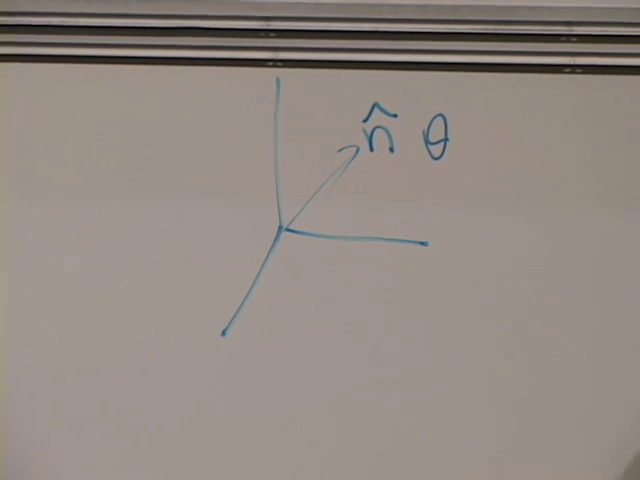
\includegraphics[width=0.58\textwidth]{lecture_03_figure_02.png}
\caption{Một trục \(\hat{\boldsymbol n}\) và một góc \(\theta\) xác định một phép quay trong không gian.}
\lectureframe{00:02:34}
\end{figure}

Một hướng trên mặt cầu đơn vị cần hai tham số, chẳng hạn như kinh độ và vĩ độ. Góc quay quanh hướng đó cung cấp tham số thứ ba. Do đó, các phép quay tạo thành một họ ba tham số. Tạm thời ta chưa cần bận tâm đến các đồng nhất hóa toàn cục do những góc sai khác nhau một \(2\pi\) gây ra; điều quan trọng ở đây là số lượng tham số cục bộ.

Mô tả bằng trục và góc có một chút dư thừa. Đảo ngược trục đồng thời đảo dấu góc cho cùng một phép toán, và những góc đủ lớn có thể được rút gọn theo modulo một vòng tròn đầy đủ. Không điều nào trong số đó làm thay đổi sự thật rằng gần phép đồng nhất, một phép quay có ba tham số biến thiên liên tục. Về sau, số đếm cục bộ ấy sẽ được đối chiếu với số tham số độc lập trong một biểu diễn ma trận.

Các tính chất của nhóm giờ đây có thể được kiểm tra lần lượt:
\begin{enumerate}
\item \emph{Tính đóng.} Thực hiện liên tiếp hai phép quay tạo ra một phép quay khác.
\item \emph{Phần tử đơn vị.} Không làm gì cả là phép quay đồng nhất.
\item \emph{Nghịch đảo.} Một phép quay qua \(\theta\) quanh \(\hat{\boldsymbol n}\) được hoàn tác bởi một phép quay qua \(-\theta\) quanh cùng trục đó.
\item \emph{Tính kết hợp.} Ba phép quay liên tiếp thỏa mãn
\[
(R_1R_2)R_3=R_1(R_2R_3).
\]
\end{enumerate}

Các phép quay không giao hoán. Một phép quay quanh trục \(x\) rồi tiếp theo là một phép quay quanh trục \(y\) nói chung cho một định hướng khác với khi thực hiện cùng hai phép toán ấy theo thứ tự ngược lại:
\begin{equation}
R_x(\alpha)R_y(\beta)\ne R_y(\beta)R_x(\alpha).
\end{equation}
Sự khác biệt trở thành bậc hai khi cả hai góc đều rất nhỏ, đó là lý do vì sao các phép quay vi phân có thể trông gần như giao hoán. Tuy vậy, toàn bộ nhóm vẫn là không abel.

Tính không giao hoán có thể được kiểm tra mà không cần bất kỳ phương trình nào. Hãy lấy một quyển sách hoặc một cái hộp, đánh dấu một mặt là mặt trước, rồi xoay nó chín mươi độ quanh trục \(x\) và sau đó chín mươi độ quanh trục \(y\). Trở về định hướng ban đầu và đảo ngược thứ tự. Mặt đã đánh dấu sẽ kết thúc theo một hướng khác. Với các góc nhỏ, độ sai khác khó thấy hơn, nhưng nó không biến mất; nó bắt đầu ở tích của hai góc nhỏ ấy.

\begin{classroomqa}
\audiencequestion{Các phép quay này là tuần tự chứ không phải đồng thời, đúng không?\lecturetimestamp{00:04:45}}
\lecturerresponse{Đúng. Phép nhân nhóm có nghĩa là một phép toán theo sau bởi một phép toán khác. Chính thứ tự của những phép quay liên tiếp ấy là điều có thể không giao hoán.}
\end{classroomqa}

Đây là nhóm không abel đầu tiên của chúng ta. Ứng dụng sau cùng không phải là màu của một vật thông thường mà là các trạng thái màu đỏ, lục và lam của một quark. Đó là một hệ nội tại ba trạng thái, và những phép biến đổi đáng quan tâm của nó trộn lẫn ba màu ấy. Các phép quay thông thường cung cấp một mô hình quen thuộc về cách một nhóm liên tục tác dụng thông qua các ma trận.

Bản thân một nhóm là trừu tượng. Để sử dụng nó trong vật lý, ta phải nói nó tác dụng lên những đối tượng nào. Một {biểu diễn} gán cho mỗi phần tử của nhóm một toán tử hoặc ma trận sao cho phép nhân các phần tử nhóm được tái hiện bởi phép nhân của các ma trận được gán. Những đối tượng vật lý khác nhau có thể mang những biểu diễn khác nhau của cùng một nhóm. Vectơ, các trạng thái spin một và các trạng thái spin một nửa sẽ cung cấp ba ví dụ.

\section{Biểu diễn vectơ ba chiều}

Cho một vectơ thông thường có các thành phần
\begin{equation}
\boldsymbol V=(V_x,V_y,V_z),\qquad V_i,\quad i=1,2,3.
\end{equation}
Ta có thể quay vectơ vật lý trong khi giữ cố định các trục, hoặc quay các trục tọa độ trong khi giữ cố định vectơ. Các quy ước là khác nhau, nhưng trong cả hai cách mô tả, các thành phần đều bị trộn bởi một ma trận \(3\times3\). Với mọi cặp trục-góc \((\hat{\boldsymbol n},\theta)\), viết
\begin{equation}
V_i'=R_{ij}(\hat{\boldsymbol n},\theta)V_j,
\label{eq:l3-vector-rotation}
\end{equation}
trong đó chỉ số lặp được lấy tổng.

Chỉ số lặp \(j\) là một nhãn giả. Phương trình ~\eqref{eq:l3-vector-rotation} có nghĩa tường minh là
\begin{equation}
V_i'=R_{i1}V_1+R_{i2}V_2+R_{i3}V_3
\end{equation}
cho mỗi thành phần đầu ra \(i\). Chỉ số tự do \(i\) cho biết thành phần nào đang được tính; \(j\) lặp được lấy tổng và có thể đổi tên mà không làm thay đổi phương trình. Giữ tách biệt hai vai trò đó sẽ ngăn được phần lớn các sai sót về chỉ số trong lập luận bảo toàn độ dài.

\begin{figure}[htbp]
\centering
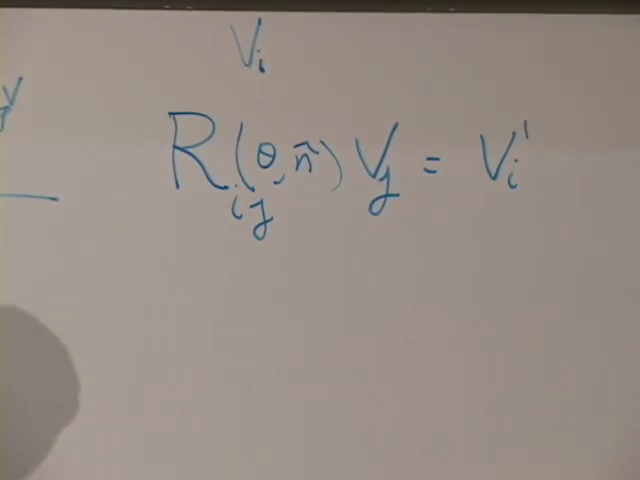
\includegraphics[width=0.68\textwidth]{lecture_03_figure_03.png}
\caption{Ma trận quay ánh xạ các thành phần vectơ ban đầu thành các thành phần sau khi quay.}
\lectureframe{00:07:41}
\end{figure}

Một phép quay đúng nghĩa bảo toàn độ dài. Tạm thời cả \(V_i\) lẫn \(R_{ij}\) đều là số thực, nên
\begin{equation}
V_i'V_i'=V_iV_i
\end{equation}
đúng với mọi vectơ. Để làm rõ điều kiện đối với ma trận, hãy viết cùng phép biến đổi đó với các chỉ số giả khác nhau:
\begin{equation}
V_i'=R_{ij}V_j,\qquad V_i'=R_{ik}V_k.
\end{equation}
Nhân rồi lấy tổng theo \(i\) cho ta
\begin{align}
V_i'V_i'
 &=R_{ij}V_jR_{ik}V_k\\
 &=R_{ij}R_{ik}V_jV_k.
\end{align}
Biểu thức này bằng \(V_jV_j\) với mọi lựa chọn của \(V\) chỉ khi
\begin{equation}
R_{ij}R_{ik}=\delta_{jk}.
\label{eq:l3-orthogonality-index}
\end{equation}
Trong ký hiệu ma trận,
\begin{equation}
R^TR=\boldsymbol 1,
\label{eq:l3-orthogonal}
\end{equation}
và do đó
\begin{equation}
R^{-1}=R^T.
\end{equation}
Phép chuyển vị chỉ đơn giản là hoán đổi hàng và cột.

Vì sao hệ số phải là \(\delta_{jk}\)? Delta Kronecker buộc \(j=k\) trong phép lấy tổng:
\begin{equation}
\delta_{jk}V_jV_k=V_1^2+V_2^2+V_3^2.
\end{equation}
Nếu \(R_{ij}R_{ik}\) khác \(\delta_{jk}\), thì một hướng nào đó hoặc một hạng chéo nào đó \(V_jV_k\) sẽ làm thay đổi độ dài. Vì đẳng thức này được yêu cầu đúng với mọi vectơ có thể có, chứ không chỉ với một vectơ được chọn, nên bản thân hệ số ma trận phải bằng ma trận đơn vị.

Phương trình ~\eqref{eq:l3-orthogonal} là điều kiện trực giao định nghĩa cho biểu diễn ma trận thực này. Phép nhân các ma trận tái hiện bảng nhân của các phép quay trong không gian. Đây không phải là biểu diễn duy nhất của nhóm quay; nó chỉ đơn thuần là biểu diễn dễ hình dung nhất.

Quan hệ nghịch đảo có một ý nghĩa hình học trực tiếp. Một phép quay có thể được hoàn tác mà không cần giải một phương trình ma trận mới: chỉ việc đổi hàng với cột. Nếu \(R_1\) và \(R_2\) biểu diễn hai phép quay, thì \(R_2R_1\) biểu diễn tác dụng liên tiếp của chúng và lại là trực giao. Vì vậy, các phép toán ma trận bảo toàn đúng cùng cấu trúc đóng, đơn vị, nghịch đảo và kết hợp đã được xác lập về mặt hình học.

\section{Spin một và biểu diễn vectơ}

Biểu diễn ba chiều cũng tác dụng lên các trạng thái lượng tử. Một hạt spin một có ba hình chiếu spin khả dĩ,
\begin{equation}
m=+1,\quad 0,\quad -1.
\end{equation}
Do đó, trạng thái spin của nó là một cột ba thành phần của các biên độ xác suất. Quay hạt, hoặc thay đổi định hướng của từ trường dùng để xác định trục spin, sẽ trộn ba biên độ ấy bởi một biểu diễn ba chiều của nhóm quay.

Số trạng thái spin tuân theo quy tắc quen thuộc \(2s+1\). Spin không có một trạng thái, spin một nửa có hai, spin một có ba, và spin ba phần hai có bốn. Vì vậy, số chiều của vectơ trạng thái thay đổi theo spin. Cùng một phép quay vật lý phải được biểu diễn bằng các ma trận có kích thước khác nhau khi nó tác dụng lên các không gian trạng thái khác nhau này.

Đối với một hạt spin một, hãy chọn cơ sở
\begin{equation}
\lvert 1,+1\rangle,qquad
\lvert 1,0\rangle,qquad
\lvert 1,-1\rangle.
\end{equation}
Một trạng thái là
\begin{equation}
\lvert\psi\rangle
=c_{+}\lvert1,+1\rangle+c_0\lvert1,0\rangle+c_{-}\lvert1,-1\rangle.
\end{equation}
Việc quay thiết bị không tạo ra trạng thái spin thứ tư; nó trộn ba hệ số \(c_+,c_0,c_-\) với nhau. Vì thế, toán tử quay tương ứng phải là một ma trận \(3\times3\).

Đối với spin một, biểu diễn này biến đổi theo cùng cách như một vectơ không gian thông thường. Đó là ý nghĩa chính xác của việc gọi một hạt spin một là hạt \emph{vectơ}: ba biên độ spin của nó và ba thành phần của một vectơ tuân theo cùng một quy luật quay. Không cần hình dung trạng thái lượng tử như một mũi tên theo nghĩa đen; phát biểu này nói về cách các thành phần của nó bị trộn lẫn.

Sự tương ứng này không phải là ngẫu nhiên. Một vectơ ba chiều và một trạng thái spin một mang các biểu diễn ba chiều tương đương của nhóm quay. Cụm từ {hạt vectơ} tóm tắt tính chất biến đổi đó. Nó không hề khẳng định rằng một trạng thái phân cực lượng tử là một mũi tên cứng tí hon ẩn bên trong hạt.

\section{Đối xứng rời rạc và liên tục}

Trước khi chuyển sang spin một nửa, sẽ hữu ích nếu phân biệt hai loại nhóm rộng. Một phép phản xạ cho một ví dụ rời rạc đơn giản. Có phép đồng nhất và có phép phản xạ \(P\); hoặc ta lật, hoặc không lật. Trái lại, một pha
\begin{equation}
e^{i\phi}
\end{equation}
phụ thuộc liên tục vào \(\phi\), và một phép quay trong không gian phụ thuộc liên tục vào trục và góc của nó. Những nhóm liên tục như vậy được gọi là \emph{nhóm Lie}, theo tên Sophus Lie; tên ấy được phát âm là \emph{Lee}. Các đối xứng liên tục sẽ là mối quan tâm chính, mặc dù các đối xứng rời rạc vẫn quan trọng.

Đối với nhóm phản xạ hai phần tử,
\begin{equation}
P^2=1.
\end{equation}
Không có một mức độ phản xạ nào điều chỉnh liên tục được giữa \(1\) và \(P\). Nhóm pha thì khác: giữa \(e^{i\phi_1}\) và \(e^{i\phi_2}\) có liên tục vô số pha khác. Các phép quay trong không gian có cùng tính liên tục đó, nhưng khác với \(U(1)\), chúng là không abel.

Spin không cho biểu diễn đơn giản nhất của nhóm quay. Một trạng thái spin-không không đổi dưới mọi phép quay, nên mỗi phần tử nhóm đều được biểu diễn bởi đồng nhất một chiều:
\begin{equation}
D^{(0)}(R)=1.
\end{equation}
Bản thân nhóm vẫn có vô số phép quay; chính biểu diễn trên trạng thái spin-không mới là tầm thường.

Sự phân biệt này giữa một nhóm và một trong các biểu diễn của nó là cốt yếu. Nhóm quay không suy sụp thành một nhóm một phần tử mỗi khi nó tác dụng lên một vô hướng. Đúng hơn, mọi phần tử của nó đều được biểu diễn bởi cùng một số \(1\) trên trạng thái vô hướng cụ thể đó.

\section{Một trạng thái spin một nửa tổng quát}

Một hệ spin một nửa có hai trạng thái cơ sở. Đối với một trục \(z\) đã chọn,
\begin{equation}
\lvert\uparrow\rangle=
\begin{pmatrix}1\\0\end{pmatrix},
\qquad
\lvert\downarrow\rangle=
\begin{pmatrix}0\\1\end{pmatrix}.
\end{equation}
Một trạng thái tổng quát là một spinor hai thành phần,
\begin{equation}
\lvert\psi\rangle=
\begin{pmatrix}\alpha_1\\\alpha_2\end{pmatrix},
\qquad
|\alpha_1|^2+|\alpha_2|^2=1.
\label{eq:l3-spinor}
\end{equation}
Các thành phần là số phức. Lựa chọn \((\alpha_1,\alpha_2)=(1,0)\) là spin lên, và \((0,1)\) là spin xuống. Một tổ hợp chuẩn hóa tổng quát mô tả một spin được phân cực dọc theo một hướng nào đó khác.

Các từ {lên} và {xuống} chỉ có ý nghĩa sau khi một trục đã được chọn. Ở đây trục đó là \(z\). Một trục đo khác có một cặp trạng thái cơ sở khác, và một trạng thái xác định là lên dọc theo một trục nói chung sẽ xuất hiện như một chồng chập trong một cơ sở khác. Quay spin vật lý hoặc quay các trục quy chiếu sẽ làm thay đổi các hệ số tương ứng.

Hai biên độ phức chứa bốn tham số thực. Điều kiện chuẩn hóa loại bỏ một tham số và pha tổng thể không liên quan về mặt vật lý loại bỏ thêm một tham số nữa, còn lại hai tham số thực. Đó đúng bằng số cần thiết để chọn một hướng trên mặt cầu. Ta không cần suy ra ánh xạ tường minh giữa \((\alpha_1,\alpha_2)\) và hướng đó để nghiên cứu các phép quay.

Pha toàn cục được loại bỏ vì
\begin{equation}
\begin{pmatrix}\alpha_1\\\alpha_2\end{pmatrix}
\quad\hbox{and}\quad
e^{i\chi}
\begin{pmatrix}\alpha_1\\\alpha_2\end{pmatrix}
\end{equation}
biểu diễn cùng một tia vật lý. Chuẩn hóa cố định tổng xác suất,
chứ không cố định một hướng trong không gian Euclid thông thường. Sau cả hai phép đồng nhất đó,
hai tham số còn lại có thể được xem là các góc cực và góc phương vị của
hướng phân cực spin.

Khi spin được quay, trạng thái của nó trở thành
\begin{equation}
\alpha_i'=U_{ij}\alpha_j,
\qquad
\begin{pmatrix}\alpha_1'\\\alpha_2'\end{pmatrix}
=
\begin{pmatrix}
U_{11}&U_{12}\\
U_{21}&U_{22}
\end{pmatrix}
\begin{pmatrix}\alpha_1\\\alpha_2\end{pmatrix}.
\label{eq:l3-spinor-transform}
\end{equation}
Vì vậy, các phép quay trong không gian có một biểu diễn ma trận hai chiều tác dụng
lên các spinor. Có một tính hai trị toàn cục trong biểu diễn này mà ta tạm gác lại;
xét cục bộ, các ma trận có các tính chất biến đổi cần dùng bên dưới.

Cặp đã biến đổi \((\alpha_1',\alpha_2')\) một lần nữa phải là một trạng thái lượng tử
có thể có. Vì vậy, câu hỏi đầu tiên về \(U\) không phải là công thức trục-góc tường minh
của nó, mà là điều kiện để nó bảo toàn chuẩn hóa của mọi spinor đầu vào.

\section{Bảo toàn xác suất và các ma trận unita}

Một phép quay phải ánh xạ một trạng thái đã chuẩn hóa thành một trạng thái đã chuẩn hóa khác:
\begin{equation}
\alpha_i^*\alpha_i=\alpha_i'^*\alpha_i'=1.
\end{equation}
Thay Phương trình~\eqref{eq:l3-spinor-transform} vào,
\begin{align}
\alpha_i'^*\alpha_i'
 &=(U_{ij}\alpha_j)^*(U_{ik}\alpha_k)\\
 &=\alpha_j^*U_{ij}^*U_{ik}\alpha_k.
\end{align}
Vì vậy, điều kiện tương tự cho vectơ thực là
\begin{equation}
(U^T)^*U=\boldsymbol 1.
\end{equation}
Phép chuyển vị rồi liên hợp phức là liên hợp Hermite,
\begin{equation}
U^\dagger=(U^T)^*,
\end{equation}
nên điều kiện bảo toàn chuẩn hóa là
\begin{equation}
U^\dagger U=\boldsymbol 1.
\label{eq:l3-unitarity}
\end{equation}

Phần liên hợp phức thêm vào là thay đổi cốt yếu duy nhất so với phép tính
vectơ thực. Với một vectơ thực, \(V_iV_i\) là một độ dài. Với một spinor,
\(\alpha_i^*\alpha_i\) là một xác suất. Cần có liên hợp phức để
làm cho xác suất ấy là số thực và không âm, nên phép chuyển vị được thay bằng
liên hợp Hermite.

Phương trình~\eqref{eq:l3-unitarity} cũng cho ngay nghịch đảo:
\begin{equation}
U^{-1}=U^\dagger.
\end{equation}
Vì vậy, phép quay nghịch đảo bảo toàn cùng một chuẩn xác suất. Cũng như với
các ma trận quay thông thường, tích của các ma trận unita vẫn là unita, nên
biểu diễn này tôn trọng phép nhân nhóm.

\begin{figure}[htbp]
\centering
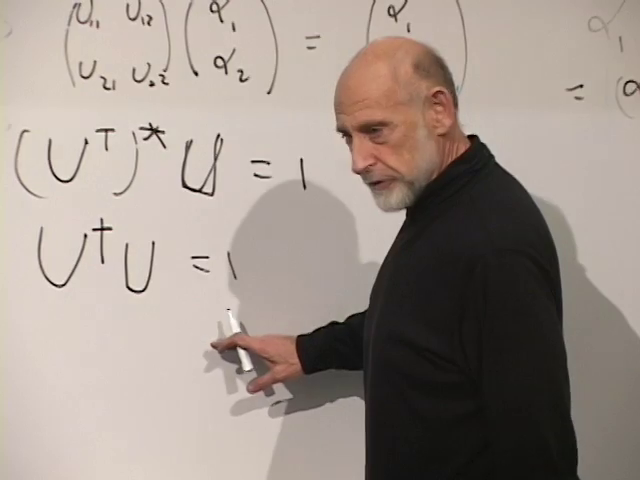
\includegraphics[width=0.62\textwidth]{lecture_03_figure_04.png}
\caption{Ma trận quay spinor thỏa mãn \(U^\dagger U=\boldsymbol 1\).}
\lectureframe{00:27:41}
\end{figure}

Các ma trận thỏa mãn Phương trình~\eqref{eq:l3-unitarity} là unita. Một ma trận phức
\(2\times2\) tổng quát ban đầu có 8 tham số thực. Tính unita là một phương trình ma trận
\(2\times2\) cung cấp 4 ràng buộc thực độc lập,
để lại 4 tham số. Một phép quay không gian chỉ có 3. Cần thêm một
ràng buộc nữa để tách biểu diễn spinor của các phép quay ra khỏi toàn bộ \(U(2)\).

Bốn ràng buộc ấy cũng có thể thấy được nếu xem hai cột của \(U\) như
hai vectơ phức. Mỗi cột phải có chuẩn đơn vị, cho 2 điều kiện thực,
và các cột phải trực giao, cho 1 điều kiện phức hay 2 điều kiện thực.
Tổng cộng là 4. Tham số thứ tư còn lại trong
\(U(2)\) hóa ra sẽ là một pha định thức toàn cục chứ không phải một phép quay không gian mới.

\section{Định thức bằng một và \texorpdfstring{\(SU(2)\)}{SU(2)}}

Điều kiện bổ sung là
\begin{equation}
\det U=1.
\label{eq:l3-det-one}
\end{equation}
Nó tương thích với phép nhân nhóm vì
\begin{equation}
\det(AB)=\det A\,\det B.
\end{equation}
Tích của hai ma trận unita có định thức bằng một lại có định thức bằng một,
và phần tử đơn vị có định thức bằng một. Các ma trận này tạo thành một nhóm con đóng.

Nghịch đảo cũng nằm trong nhóm con. Nếu \(\det U=1\), thì
\begin{equation}
\det U^{-1}=\frac{1}{\det U}=1.
\end{equation}
Vì vậy, áp đặt điều kiện định thức bằng một không loại bỏ phần tử đơn vị,
không phá hỏng tính đóng, cũng không làm mất các nghịch đảo. Nó nhất quán chọn ra một nhóm có ít hơn một tham số liên tục.

Chỉ riêng tính unita đã suy ra
\begin{equation}
\det(U^\dagger U)=
(\det U)^*\det U
=|\det U|^2=1.
\end{equation}
Nó không buộc \(\det U\) phải là \(+1\) hay \(-1\). Định thức unita tổng quát
có thể là bất kỳ pha nào:
\begin{equation}
\det U=e^{i\phi},
\qquad
\det U^\dagger=e^{-i\phi}.
\end{equation}
Điều kiện~\eqref{eq:l3-det-one} cố định pha vốn dĩ tự do này và loại bỏ một
tham số thực.

\begin{classroomqa}
\audiencequestion{Liệu \(U^\dagger U=\boldsymbol 1\), nếu không có điều kiện định thức bằng một, có buộc \(\det U^\dagger\) bằng \(\det U\) hay chỉ có thể là \(+1\) hoặc \(-1\) không?\lecturetimestamp{00:31:21}}
\lecturerresponse{Không. Hai định thức ấy là liên hợp phức của nhau. Chúng có thể là \(e^{i\phi}\) và \(e^{-i\phi}\), mà tích của chúng bằng một. Khi đó ràng buộc unita đặc biệt cố định cả hai bằng một.}
\end{classroomqa}

Các ma trận unita \(n\times n\) tạo thành \(U(n)\). Với \(n=1\), một ma trận unita
chỉ đơn giản là pha \(e^{i\phi}\), cho ta \(U(1)\). Nhóm con định thức bằng một
là nhóm \emph{unita đặc biệt},
\begin{equation}
SU(n)=\{U\in U(n):\det U=1\}.
\end{equation}
Spinor hai thành phần biến đổi dưới tác dụng của \(SU(2)\), một nhóm có 3 tham số.

Ký hiệu ghi lại cả hai ràng buộc: \(U\) nghĩa là unita, còn \(S\)
nghĩa là đặc biệt, tức định thức bằng một. Các nhóm unita đặc biệt này xuất hiện
lặp đi lặp lại vì chúng bảo toàn một tích vô hướng phức đồng thời loại trừ
pha chung độc lập do định thức mang theo.

Xét cục bộ, \(SU(2)\) có cùng đại số quay và cấu trúc phép nhân cần thiết
để quay các trạng thái spin một nửa. Xét toàn cục, phải nhớ đến sự tinh tế đã
tạm hoãn: \(SU(2)\) là phủ đôi của nhóm quay thông thường
\(SO(3)\), nên hai phần tử của \(SU(2)\) tương ứng với một phép quay không gian.
\editorialnote{Phát biểu bằng phủ đôi làm rõ tính hai trị đã được nhắc đến nhưng chưa được triển khai trong nguồn.}

\section{Các phép quay vô cùng bé và các ma trận Pauli}

\begin{classroomqa}
\audiencequestion{Các ma trận spin, hay ma trận Pauli, đi vào cấu trúc này ở đâu?\lecturetimestamp{00:33:16}}
\lecturerresponse{Chúng xuất hiện khi một phần tử nhóm được lấy rất gần phần tử đơn vị, tương ứng với một phép quay qua một góc rất nhỏ. Chúng là các bộ sinh của những phép quay vô cùng bé đó.}
\end{classroomqa}

Bắt đầu với
\begin{equation}
U=\boldsymbol 1+\epsilon M+O(\epsilon^2),
\label{eq:l3-small-u-anti}
\end{equation}
trong đó \(\epsilon\) là thực và nhỏ. Khi đó
\begin{equation}
U^\dagger=\boldsymbol 1+\epsilon M^\dagger+O(\epsilon^2),
\end{equation}
và tính unita cho
\begin{align}
U^\dagger U
 &=\boldsymbol 1+\epsilon(M^\dagger+M)+O(\epsilon^2).
\end{align}
Ở bậc nhất,
\begin{equation}
M^\dagger=-M.
\end{equation}
Vì vậy ma trận \(M\) trong Phương trình~\eqref{eq:l3-small-u-anti} là
phản Hermite.

Chỉ giữ lại các hạng tuyến tính theo \(\epsilon\). Tích
\(\epsilon^2M^\dagger M\) bị bỏ đi vì nó thuộc bậc hai. Đây là
ưu điểm của việc làm việc gần phần tử đơn vị: các điều kiện nhóm phi tuyến
trở thành các điều kiện tuyến tính lên các bộ sinh của chúng.

Thuận tiện hơn nếu tách một thừa số \(i\):
\begin{equation}
U=\boldsymbol 1+i\epsilon H+O(\epsilon^2).
\label{eq:l3-small-u-herm}
\end{equation}
Liên hợp phức biến \(i\) thành \(-i\), nên
\begin{equation}
U^\dagger=\boldsymbol 1-i\epsilon H^\dagger+O(\epsilon^2).
\end{equation}
Bây giờ
\begin{equation}
U^\dagger U
=\boldsymbol 1+i\epsilon(H-H^\dagger)+O(\epsilon^2),
\end{equation}
và tính unita ở bậc nhất đòi hỏi
\begin{equation}
H^\dagger=H.
\end{equation}
Khi đã tách thừa số \(i\) ra, bộ sinh là Hermite.

Phép nhân với \(i\) không làm thay đổi các ma trận vô cùng bé được phép; nó
chỉ thay đổi quy ước dùng để gọi tên bộ sinh. Trong vật lý người ta thường
chọn các bộ sinh Hermite vì các trị riêng của chúng là thực và vì các đại lượng quan sát tương ứng, như mômen góc, là Hermite.

Điều kiện định thức bằng một dẫn đến tính không vết\editorialnote{Trong lời nói, khai triển định thức thoáng làm rối các chỉ số dưới. Số hạng tuyến tính đã hiệu chỉnh là \(A_{11}+A_{22}=\operatorname{tr}A\); các tích ngoài đường chéo chỉ bắt đầu ở bậc hai.}. Với một ma trận
\(2\times2\) nhỏ \(A\),
\begin{equation}
\det(\boldsymbol 1+A)
=
\det
\begin{pmatrix}
1+A_{11}&A_{12}\\
A_{21}&1+A_{22}
\end{pmatrix}.
\end{equation}
Khai triển ra,
\begin{align}
\det(\boldsymbol 1+A)
 &=(1+A_{11})(1+A_{22})-A_{12}A_{21}\\
 &=1+A_{11}+A_{22}+O(A^2)\\
 &=1+\operatorname{tr}A+O(A^2).
\end{align}
Áp dụng điều này cho \(A=i\epsilon H\),
\begin{equation}
\det U=1+i\epsilon\,\operatorname{tr}H+O(\epsilon^2).
\end{equation}
Vì vậy, \(\det U=1\) đòi hỏi
\begin{equation}
\operatorname{tr}H=0.
\end{equation}
Điều kiện vết loại bỏ đúng bộ sinh tỉ lệ với
ma trận đơn vị. Một ma trận Hermite \(2\times2\) tổng quát có 4 tham số thực: 2
phần tử đường chéo thực và 1 phần tử ngoài đường chéo phức. Vết của nó cố định một tổ hợp thực, để lại 3. Điều này khớp với 3 trục mà quanh đó có thể thực hiện một phép quay không gian vô cùng bé.

Vì thế, các bộ sinh vô cùng bé của \(SU(2)\) là các ma trận Hermite \(2\times2\)
không vết. Ba ma trận Pauli tạo thành một cơ sở:
\begin{equation}
\begin{aligned}
\sigma_x&=
\begin{pmatrix}0&1\\1&0\end{pmatrix},
&
\sigma_y&=
\begin{pmatrix}0&-i\\i&0\end{pmatrix},
\\[0.4em]
\sigma_z&=
\begin{pmatrix}1&0\\0&-1\end{pmatrix}.
\end{aligned}
\end{equation}
Mọi bộ sinh đều có thể viết thành
\begin{equation}
H=a_x\sigma_x+a_y\sigma_y+a_z\sigma_z.
\end{equation}
Một phép quay nhỏ quanh trục \(x\) chọn \(\sigma_x\); một phép quay quanh
trục \(y\) chọn \(\sigma_y\); và một phép quay quanh bất kỳ trục nào khác chọn
tổ hợp tuyến tính tương ứng. Trong đơn vị với \(\hbar=1\), các toán tử
spin là
\begin{equation}
S_i=\frac{\sigma_i}{2}.
\end{equation}

Chẳng hạn, một trục nằm chính giữa \(x\) và \(y\) dùng một bộ sinh
tỉ lệ với
\begin{equation}
\frac{\sigma_x+\sigma_y}{\sqrt2}.
\end{equation}
Hướng của vectơ hệ số
\((a_x,a_y,a_z)\) chọn trục quay, còn độ lớn của nó kết hợp với
\(\epsilon\) để đặt góc nhỏ. Đây là mối liên hệ giữa các ma trận spin gặp trong các giao hoán tử mômen góc và các toán tử quay hữu hạn. Cụ thể,
\begin{equation}
[S_x,S_y]=iS_z
\end{equation}
và các hoán vị chu kỳ của nó mã hóa tính không giao hoán đã thấy về mặt hình học.
Phép quay hữu hạn chuẩn thu được bằng cách lấy mũ bộ sinh vô cùng bé\editorialnote{Công thức phép quay hữu hạn dạng hàm mũ là phần hoàn chỉnh chuẩn của cách xây dựng vô cùng bé; nguồn chỉ suy ra các điều kiện của bộ sinh và cơ sở ma trận Pauli của chúng.},
\begin{equation}
U(\hat{\boldsymbol n},\theta)
=\exp\left(-\frac{i\theta}{2}\,
\hat{\boldsymbol n}\cdot\boldsymbol\sigma\right).
\end{equation}
\section{Không gian màu ba trạng thái}

Việc kết hợp các biểu diễn có thể để sau. Giờ ta rời spin trong không gian và quay lại
màu của quark. Một quark vẫn có spin một nửa, nhưng màu của nó là một
độ tự do ba trạng thái độc lập:
\begin{equation}
\lvert r\rangle,\qquad
\lvert g\rangle,\qquad
\lvert b\rangle.
\end{equation}
Một trạng thái màu tổng quát là
\begin{equation}
\begin{aligned}
\lvert q\rangle_{\mathrm{color}}
={}&
\alpha_r\lvert r\rangle
+\alpha_g\lvert g\rangle
+\alpha_b\lvert b\rangle,
\\
&|\alpha_r|^2+|\alpha_g|^2+|\alpha_b|^2=1.
\end{aligned}
\end{equation}
Tương đương,
\begin{equation}
q=
\begin{pmatrix}
\alpha_r\\
\alpha_g\\
\alpha_b
\end{pmatrix}.
\end{equation}
Bình phương độ lớn là các xác suất để có đỏ, lục và lam trong một
cơ sở màu đã chọn. Cùng ký hiệu bộ ba ấy cũng có thể gom ba toán tử trường quark,
\begin{equation}
\psi=
\begin{pmatrix}
\psi_r\\
\psi_g\\
\psi_b
\end{pmatrix}.
\end{equation}

Spin và màu phải được giữ tách biệt về mặt khái niệm. Nhãn spin cho biết trạng thái
biến đổi như thế nào dưới các phép quay của không gian vật lý. Nhãn màu cho biết
nó biến đổi như thế nào dưới một đối xứng nội tại không quay phòng thí nghiệm.
Một trạng thái quark mang cả hai nhãn, dù trong thảo luận hiện tại spin được
lược bỏ để tập trung vào màu.

Viết ba toán tử trường trong một cột không chỉ là việc ghi chép. Nó cho phép
phát biểu đối xứng trong một phương trình ma trận duy nhất. Một phép biến đổi
có thể biến một trường đỏ thành một tổ hợp tuyến tính của các trường đỏ, lục và lam,
giống như một phép quay không gian biến một thành phần vectơ thành một tổ hợp tuyến
tính của các thành phần khác.

Trước hết có thể hình dung các phép biến đổi rời rạc hoán đổi hai màu. Đối xứng
lớn hơn chứa các sự pha trộn liên tục của cả ba. Một ma trận hoán đổi đơn giản
có thể cần kèm theo một pha để làm cho định thức của nó bằng một; khi đó phép
hoán đổi được nhúng vào nhóm unita đặc biệt.

Đối với hai trạng thái cơ sở, phép hoán đổi thuần túy được biểu diễn bởi
\begin{equation}
X=
\begin{pmatrix}0&1\\1&0\end{pmatrix},
\qquad
\det X=-1.
\end{equation}
Nhân toàn bộ ma trận với \(i\) cho
\begin{equation}
\det(iX)=i^2\det X=1.
\end{equation}
Vì vậy, phép hoán đổi rời rạc có thể xuất hiện như một phần tử cụ thể của
nhóm liên tục lớn hơn một khi pha được chọn nhất quán.

\begin{classroomqa}
\audiencequestion{Một ma trận chỉ đơn thuần hoán đổi hai trạng thái cơ sở có định thức sai đối với \(SU(2)\) không?\lecturetimestamp{00:43:46}}
\lecturerresponse{Phép hoán đổi thuần túy có định thức \(-1\). Một thừa số thích hợp của \(i\) cung cấp một đại diện có định thức bằng một, nên phép hoán đổi có thể được bao gồm trong các phép biến đổi unita đặc biệt liên tục.}
\end{classroomqa}

\section{\texorpdfstring{\(SU(3)\)}{SU(3)} và tám bộ sinh màu}

Phép biến đổi màu liên tục là
\begin{equation}
\begin{aligned}
q'&=Uq,
&
U^\dagger U&=\boldsymbol 1,
\\
\det U&=1,
&
U&\in SU(3).
\end{aligned}
\label{eq:l3-su3-action}
\end{equation}
Toán học ở đây là cùng một cấu trúc unita đặc biệt được dùng cho spinor,
nhưng nay \(U\) là \(3\times3\). Đây không phải là một phép quay của không gian vật lý. Nó là
một phép quay trong không gian màu nội tại.

Tính unita bảo toàn chuẩn hóa của trạng thái màu:
\begin{equation}
q^\dagger q
=|\alpha_r|^2+|\alpha_g|^2+|\alpha_b|^2.
\end{equation}
Định thức bằng một loại bỏ hướng pha chung \(U(1)\) khỏi sự pha trộn liên tục.
Các ma trận thu được có thể thực hiện các phép hoán đổi đơn giản, các thay đổi
pha tương đối và các chồng chập liên tục thực sự mà vẫn nằm trong một nhóm đóng.

Việc đếm tham số là trực tiếp. Một ma trận phức \(3\times3\) có 9
phần tử phức, tức 18 tham số thực. Phương trình ma trận
\(U^\dagger U=\boldsymbol 1\) áp đặt 9 điều kiện thực. Điều kiện định thức bằng một
loại bỏ thêm 1 tham số nữa:
\begin{equation}
\dim SU(3)=18-9-1=8.
\end{equation}
Vì vậy, \(SU(3)\) có 8 bộ sinh vô cùng bé độc lập.

9 điều kiện thực của tính unita lại có thể được hiểu theo các cột của
\(U\). Ba cột phức mỗi cột đều phải có chuẩn đơn vị, và mọi cặp
đều phải trực giao. Các điều kiện này loại bỏ 9 trong số 18 tham số thực
ban đầu. Pha định thức loại bỏ tham số thứ 10, còn lại 8.
Đây là bản tương tự ba trạng thái của cách đếm \(8-4-1=3\) cho \(SU(2)\).

Sự xuất hiện của con số tám chính là cùng một sự kiện mà rốt cuộc tạo ra tám loại gluon. Nói rằng không có chín gluon vì ràng buộc định thức đã loại bỏ một phương chỉ là một mẹo ghi nhớ. Chính xác hơn, chín ma trận màu-phản màu phân rã thành một hướng singlet màu, tỉ lệ với ma trận đơn vị, và tám hướng không vết. Tám phần tử sinh không vết tạo thành cấu trúc màu adjoint mà các gluon QCD mang.\editorialnote{Cách trình bày singlet-cộng-octet là phiên bản chính xác tiêu chuẩn của nhận xét về định thức cố ý mang tính gợi ý trong văn bản gốc; việc xây dựng trường chuẩn của nó được để lại cho sau.}

Ở giai đoạn này, mối liên hệ với tám gluon mới là một dấu mốc chỉ đường, chưa phải là một suy dẫn đầy đủ. Để thu được các hạt chuẩn, ta phải nâng đối xứng màu thành đối xứng cục bộ và xác định các trường bù. Điều mà việc đếm tham số đã cho thấy là có tám hướng độc lập mà theo đó một phép biến đổi màu \(SU(3)\) có thể bắt đầu lệch khỏi phần tử đơn vị.

\section{Đối xứng màu ràng buộc QCD}

Phát biểu đối xứng cơ bản là vật lý bất biến dưới phép biến đổi màu trong Phương trình~\eqref{eq:l3-su3-action}. Đây là đối xứng nội tại trung tâm của sắc động lực học lượng tử. Việc trộn các thành phần màu tương tự về mặt hình thức với việc trộn các biên độ spin lên và spin xuống, và đến lượt mình các phép biến đổi spinor đó lại liên hệ với các phép quay của những phương trong không gian, nhưng không được nhầm lẫn ba không gian này với nhau.

Gọi màu là một đối xứng có nghĩa là thay đổi cơ sở màu không làm thay đổi các dự đoán vật lý. Đỏ, xanh lục và xanh lam là những tên gọi tiện dụng cho ba vectơ cơ sở, chứ không phải ba sắc tố có thể quan sát được. Một phép quay \(SU(3)\) tác dụng đồng thời lên các thành phần màu phải giữ nguyên dạng của các định luật. Tính bất biến này không phải là một nét thẩm mỹ tùy chọn; nó là nguyên lý tổ chức của QCD.

Đối xứng ràng buộc Lagrangian. Trong ví dụ \(U(1)\) trước đó, tính bất biến dưới một phép biến đổi pha chung đã buộc các hạng được phép phải chứa các thừa số cân bằng của một trường và liên hợp của nó. Trong QCD, tương tự, mọi hạng đều phải bất biến dưới phép biến đổi màu \(SU(3)\). Yêu cầu đó kéo theo các hệ quả đối với các tương tác, các đại lượng bảo toàn và dạng của trường gluon.

Giả sử một hạng được đề xuất mang một chỉ số màu tự do. Dưới Phương trình~\eqref{eq:l3-su3-action}, chỉ số đó quay, nên bản thân hạng ấy không thể bất biến. Các hạng được phép phải co các chỉ số màu thành những tổ hợp bất biến hoặc dùng các trường chuẩn có phép biến đổi bù lại sự thay đổi đó. Đây là hiệu lực thực tiễn của nguyên lý đối xứng: nó loại trừ các ghép tùy ý và sắp xếp những tương tác còn lại.

Việc xây dựng đầy đủ QCD đòi hỏi thêm một bước nữa: phép biến đổi màu phải được cho phép biến thiên từ điểm này sang điểm khác, và trường chuẩn phải bù cho sự thay đổi cục bộ đó.\editorialnote{Việc địa phương hóa đối xứng màu là cách hoàn chỉnh thông thường trong lý thuyết chuẩn đối với phần thảo luận toàn cục về \(SU(3)\); điều đó không được triển khai trong bài giảng gốc này.} Sự phát triển đó thuộc về giai đoạn tiếp theo. Hiện tại, cấu trúc cốt yếu đã có: một triplet màu chịu tác dụng của một đối xứng unita đặc biệt ba trạng thái với tám phần tử sinh.

Phép tính đã đi sâu vào lý thuyết nhóm đến mức cần thiết cho lúc này. Ta bắt đầu từ các phép quay có thể vẽ trong không gian thông thường, chuyển sang các ma trận tác dụng lên vectơ và spinor, rồi sau đó áp dụng lại cùng lập luận ấy trong một không gian màu nội tại. Ở bước tiếp theo, ta có thể trở lại vật lý hạt với khuôn khổ toán học đã sẵn có, thay vì bắt hình thức luận phải gánh toàn bộ câu chuyện vật lý ngay lập tức.

\chapter{Biểu diễn màu, hadron và sự giam hãm}

\paragraph{Một đoạn dừng ngắn mở đầu.}
Trước khi quay lại lý thuyết nhóm, xin cho phép một lời quảng cáo trơ trẽn. \emph{The
Black Hole War} kể câu chuyện về cuộc tranh luận kéo dài với Stephen Hawking về việc liệu hố đen có phá hủy thông tin lượng tử hay không. Nó cũng ghi lại phần nào sự tàn nhẫn rất riêng của các nhà vật lý lý thuyết: không chỉ con mèo của Schrodinger, mà cả những con cá của Susskind và chuyến đi xui xẻo của chúng xuống bồn cầu. Xong nghĩa vụ đó, ta quay lại với Alice và Bob. Alice vẫn đang khổ sở, vì Bob vẫn bắt cô ấy học lý thuyết nhóm.

\lectureoverview{Một đối xứng trở thành vật lý thông qua tác dụng của nó lên các trạng thái. Ta bắt đầu với các phép quay để giới thiệu các biểu diễn và các toán tử sinh, rồi lặp lại cấu trúc đó cho màu \(SU(3)\). Các biểu diễn màu kết hợp thành các hadron, và động lực học của chúng giải thích vì sao không bao giờ quan sát thấy màu cô lập.}

\section{Nhóm và các đối tượng mà nó tác dụng lên}

Trong mọi thảo luận về đối xứng đều có hai ý niệm. Thứ nhất là một nhóm trừu tượng: một tập hợp các phép toán với luật nhân, phần tử đơn vị và các phần tử nghịch đảo. Thứ hai là các đối tượng mà những phép toán ấy tác dụng lên. Có thể phân biệt hai ý niệm này, nhưng trong vật lý thì không thể tách chúng rời nhau. Một đối xứng có ý nghĩa vì nó biến đổi các trạng thái vật lý, các trường, các tọa độ hoặc các đại lượng quan sát được.

\begin{classroomqa}
\audiencequestion{Một nhóm vừa được mô tả như một bảng nhân trừu tượng, vừa như các ma trận tác dụng lên các đối tượng vật lý. Hai phần đó có thể tách rời nhau không?
\lecturetimestamp{00:01:58}}
\lecturerresponse{Đó là hai mức mô tả khác nhau, nhưng chúng liên hệ hoàn toàn với nhau. Một phép quay tồn tại như một phép toán trừu tượng trước khi ta chỉ rõ nó quay cái gì. Khi đó vật lý hỏi chính phép toán ấy tác dụng thế nào lên các trạng thái và các đại lượng thích hợp với một hệ cụ thể. Các ma trận cung cấp tác dụng cụ thể đó đồng thời vẫn bảo toàn luật nhân trừu tượng.}
\end{classroomqa}

Các phép quay trong không gian cho ví dụ sáng sủa nhất. Trong cơ học cổ điển, cùng một phép quay có thể tác dụng lên tọa độ của hạt, lên phương của một nam châm, hoặc lên bất kỳ vectơ nào khác. Trong cơ học lượng tử, các trạng thái sống trong một không gian vectơ tuyến tính, nên một phép quay được biểu diễn bởi một toán tử tuyến tính trên không gian đó. Nếu \(g\) ký hiệu một phần tử nhóm trừu tượng và \(D(g)\) là đại diện ma trận của nó, thì tính nhất quán có nghĩa là
\begin{equation}
D(g_1g_2)=D(g_1)D(g_2),
\qquad
D(e)=\boldsymbol 1.
\end{equation}
Các ma trận không nhất thiết phải trông giống các phép toán trừu tượng, nhưng phép nhân của chúng phải tái tạo phép nhân của nhóm.
\editorialnote{Phương trình đồng cấu này viết tường minh sự tương ứng giữa phép nhân nhóm và phép nhân ma trận đã được mô tả bằng lời trong nguồn.}

Kích thước của ma trận được quyết định bởi không gian trạng thái, chứ không chỉ bởi riêng nhóm trừu tượng. Nếu ta chỉ giữ lại spin của một electron, có hai khả năng trực giao, spin lên và spin xuống, và một trạng thái là một vectơ cột hai thành phần. Vì thế các phép quay tác dụng thông qua các ma trận \(2\times2\). Đối với hai đối tượng spin một phần hai, có bốn trạng thái cơ sở,
\begin{equation}
\ket{\uparrow\uparrow},\qquad
\ket{\uparrow\downarrow},\qquad
\ket{\downarrow\uparrow},\qquad
\ket{\downarrow\downarrow},
\end{equation}
và tác dụng cảm sinh lên không gian kết hợp là bốn chiều.

Dãy quen thuộc là
\begin{equation}
\begin{array}{c|c|c}
\text{spin} & \text{number of states} & \text{matrix dimension}\\
\hline
0 & 1 & 1\times1\\
\frac12 & 2 & 2\times2\\
1 & 3 & 3\times3\\
\frac32 & 4 & 4\times4
\end{array}
\end{equation}
và cứ thế tiếp tục. Một trạng thái spin không cho biểu diễn tầm thường: mọi phép quay đều để nó yên. Ma trận một nhân một đơn giản là \(1\). Một trạng thái spin một có ba thành phần, và các ma trận quay của nó là các phép quay vectơ ba chiều quen thuộc. Tổng quát hơn, spin \(j\) có \(2j+1\) trạng thái.

Biểu diễn cũng có thể vô hạn chiều. Nếu ta mô tả toàn bộ chuyển động quỹ đạo của một electron thay vì chỉ spin của nó, thì một trạng thái chứa một biên độ cho mọi vị trí, hay tương đương là cho mọi động lượng. Khi đó toán tử quay tác dụng trên một không gian hàm sóng vô hạn chiều. Vì vậy, cùng một nhóm quay trừu tượng có các biểu diễn tầm thường, hai chiều, ba chiều và vô hạn chiều. Đây là sự kiện mà ta sẽ dùng lại khi chuyển thảo luận từ spin sang màu.

\section{Vì sao các phép quay spin là unita đặc biệt}

Giờ quay lại spin của một electron đơn lẻ và bỏ qua chuyển động quỹ đạo của nó. Một phép quay được biểu diễn bởi một ma trận unita \(2\times2\) \(U\),
\begin{equation}
U^\dagger U=\boldsymbol 1,
\qquad
U^{-1}=U^\dagger.
\label{eq:l4-unitarity}
\end{equation}
Phép biến đổi nghịch đảo phải khử phép quay, và tính unita bảo toàn chuẩn, do đó bảo toàn mọi xác suất.

Một ma trận phức tổng quát \(2\times2\) có bốn phần tử phức, tức tám tham số thực. Phương trình~\eqref{eq:l4-unitarity} áp đặt bốn điều kiện thực độc lập, còn lại bốn tham số. Một phép quay không gian thông thường chỉ có ba: hai tham số chọn trục và một chọn góc. Vì thế ma trận unita chứa thừa một pha. Điều kiện bổ sung là
\begin{equation}
\det U=1.
\label{eq:l4-det-one}
\end{equation}
Khi đó phép đếm là
\begin{equation}
8-4-1=3.
\end{equation}

Điều kiện định thức bằng một được bảo toàn dưới phép nhân vì
\begin{equation}
\det(AB)=\det A\,\det B.
\end{equation}
Nếu hai ma trận đều có định thức bằng một thì tích của chúng cũng vậy. Điều đó cũng tương thích với tính unita. Lấy định thức của Phương trình~\eqref{eq:l4-unitarity} ta được
\begin{equation}
1=\det(U^\dagger U)
=\det(U^\dagger)\det U
=(\det U)^*\det U.
\end{equation}
Do đó, định thức của một ma trận unita nằm trên đường tròn đơn vị,
\begin{equation}
\det U=e^{i\phi}.
\end{equation}

\begin{classroomqa}
\audiencequestion{Tính unita có đòi hỏi định thức phải là số thực không?
\lecturetimestamp{00:12:10}}
\lecturerresponse{Không. Tính unita chỉ đòi hỏi môđun bằng một. Định thức có thể là bất kỳ pha thuần túy nào \(e^{i\phi}\). Đối với một ma trận hai chiều, nhân \(U\) với \(e^{-i\phi/2}\) sẽ loại bỏ pha chung đó và tạo ra một ma trận có định thức bằng một.}
\end{classroomqa}

Thật vậy, nếu
\begin{equation}
V=e^{-i\phi/2}U,
\end{equation}
thì \(V\) vẫn unita và
\begin{equation}
\det V=e^{-i\phi}\det U=1.
\end{equation}
Các ma trận unita có định thức bằng một tạo thành \(SU(2)\).

Có một điểm tinh tế. Rất dễ nói rằng \(SU(2)\) đơn giản chính là nhóm các phép quay trong không gian ba chiều, nhưng sự tương ứng là hai đối một. Các ma trận \(U\) và \(-U\) tác dụng khác nhau lên một spinor, nhưng chúng tương ứng với cùng một phép quay của một vectơ thông thường. Vì thế
\begin{equation}
SU(2)/\{\boldsymbol 1,-\boldsymbol 1\}\simeq SO(3).
\end{equation}
Đối với thảo luận hiện tại, điều quan trọng là cấu trúc nhân cục bộ và ba toán tử sinh, nhưng phủ đôi này giải thích tính hai giá trị của các phép quay spin một phần hai.

\section{Các biến đổi vô cùng bé và các toán tử sinh của chúng}

Một phép quay hữu hạn có thể được xây dựng từ nhiều phép quay rất nhỏ. Một phần tử nhóm gần với đơn vị được gọi là vô cùng bé, và trong một nhóm liên thông, biết mọi hướng vô cùng bé là đủ để dựng lại các biến đổi hữu hạn bằng phép nhân lặp lại. Quan trọng hơn đối với vật lý, các toán tử sinh ra những biến đổi vô cùng bé này chính là các đại lượng bảo toàn gắn với đối xứng.

Viết một phần tử gần đơn vị dưới dạng
\begin{equation}
U=\boldsymbol 1+i\epsilon T,
\qquad |\epsilon|\ll1.
\label{eq:l4-infinitesimal-u}
\end{equation}
Hệ số \(i\) là một quy ước thuận tiện. Thế vào điều kiện unita và bỏ các hạng bậc \(\epsilon^2\), ta được
\begin{align}
(\boldsymbol 1+i\epsilon T)
(\boldsymbol 1-i\epsilon T^\dagger)&=\boldsymbol 1,
\\
i\epsilon(T-T^\dagger)&=0,
\\
T&=T^\dagger.
\label{eq:l4-hermitian-generator}
\end{align}
Toán tử sinh là Hermite, đúng như một đại lượng quan sát trong cơ học lượng tử phải vậy.

\begin{figure}[htbp]
\centering
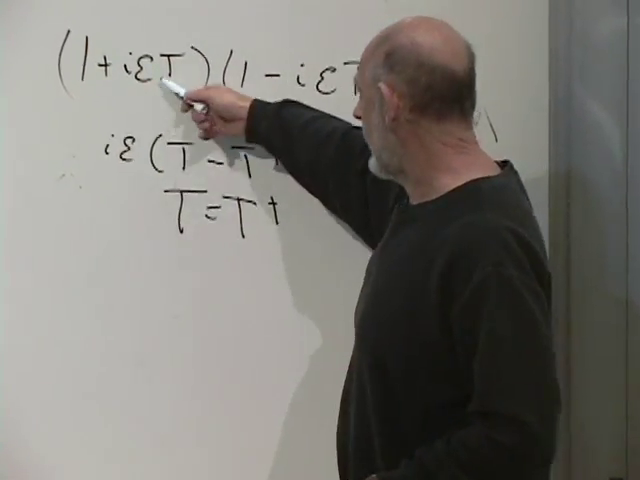
\includegraphics[width=0.62\textwidth]{lecture_04_figure_03.png}
\caption{Phép tính unita gần đơn vị kết thúc ở \(T=T^\dagger\).}
\lectureframe{00:23:28}
\end{figure}

Đối với các phép quay không gian, có ba toán tử sinh độc lập tuyến tính vì có ba trục độc lập cho các phép quay vô cùng bé. Một phép quay nhỏ quanh một hướng bất kỳ được ghép từ các phép quay nhỏ quanh \(x\), \(y\) và \(z\). Các toán tử sinh tương ứng là các toán tử mômen góc \(J_x,J_y,J_z\). Các giao hoán tử của chúng mã hóa tính không giao hoán của các phép quay,
\begin{equation}
[J_i,J_j]=i\epsilon_{ijk}J_k.
\label{eq:l4-angular-momentum-algebra}
\end{equation}
Từ đó, các phép quay vô cùng bé lặp lại dựng nên một phép quay hữu hạn.

Ta đã dùng tính unita nhưng vẫn chưa dùng điều kiện định thức bằng một. Với mọi ma trận nhỏ \(m\),
\begin{equation}
\det(\boldsymbol 1+\epsilon m)
=1+\epsilon\,\operatorname{tr}m+O(\epsilon^2).
\label{eq:l4-det-expansion}
\end{equation}

\begin{figure}[htbp]
\centering
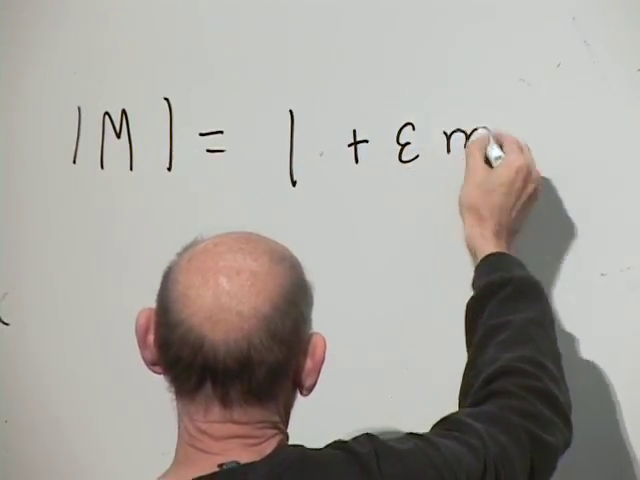
\includegraphics[width=0.62\textwidth]{lecture_04_figure_02.png}
\caption{Khai triển định thức bậc nhất ở bước đầu trên bảng.}
\lectureframe{00:21:51}
\end{figure}

Áp dụng Phương trình~\eqref{eq:l4-det-expansion} cho Phương trình~\eqref{eq:l4-infinitesimal-u},
\begin{equation}
\det U
=1+i\epsilon\,\operatorname{tr}T+O(\epsilon^2).
\end{equation}
Vì thế điều kiện unita đặc biệt đòi hỏi
\begin{equation}
\operatorname{tr}T=0.
\label{eq:l4-traceless-generator}
\end{equation}
Các toán tử sinh của \(SU(2)\) chính xác là các ma trận Hermite \(2\times2\) không vết. Không gian vectơ đó có số chiều là ba. Một cơ sở chuẩn được cho bởi các ma trận Pauli,
\begin{equation}
\begin{aligned}
\sigma_x&=
\begin{pmatrix}0&1\\1&0\end{pmatrix},
&
\sigma_y&=
\begin{pmatrix}0&-i\\i&0\end{pmatrix},
\\[0.4em]
\sigma_z&=
\begin{pmatrix}1&0\\0&-1\end{pmatrix}.
\end{aligned}
\end{equation}
Đối với biểu diễn spin một phần hai, có thể lấy \(J_i=\sigma_i/2\), nên một phép quay hữu hạn qua góc \(\theta\) quanh \(\hat{\boldsymbol n}\) là
\begin{equation}
U(\hat{\boldsymbol n},\theta)
=\exp\!\left(-i\theta\,
\hat{\boldsymbol n}\cdot\boldsymbol\sigma/2\right).
\end{equation}
\editorialnote{Số mũ hữu hạn là sự hoàn tất tiêu chuẩn của phần thảo luận về toán tử sinh vô cùng bé. Nguồn nhấn mạnh các phép quay nhỏ lặp lại hơn là viết công thức này tường minh.}

\begin{classroomqa}
\audiencequestion{Vậy có ba ma trận \(2\times2\) Hermite không vết độc lập phải không?
\lecturetimestamp{00:24:07}}
\lecturerresponse{Đúng. Chúng là ba ma trận Pauli. Với các ma trận unita đặc biệt \(3\times3\), số tương ứng là tám, và một cơ sở quy ước được cho bởi tám ma trận Gell-Mann.}
\end{classroomqa}

\begin{classroomqa}
\audiencequestion{Số tám đó có phải cũng chính là ``tám'' trong Bát đạo và tám gluon không?
\lecturetimestamp{00:24:43}}
\lecturerresponse{Toán học là cùng một loại lý thuyết biểu diễn \(SU(3)\), nhưng phải chỉ rõ đối xứng \(SU(3)\) nào đang tác dụng. Đối xứng hương vị kiểu Bát đạo trong lịch sử không phải là màu \(SU(3)\). Tám gluon thuộc biểu diễn adjoint của màu \(SU(3)\).}
\end{classroomqa}

\section{Từ SU(2) đến SU(3) màu}

Bây giờ tăng kích thước ma trận từ \(2\times2\) lên \(3\times3\). Một ma trận phức tổng quát
\(3\times3\) có chín phần tử phức, nên có mười tám tham số thực.
Điều kiện \(U^\dagger U=\boldsymbol 1\) cung cấp chín ràng buộc thực,
và \(\det U=1\) loại thêm một điều kiện nữa. Do đó
\begin{equation}
18-9-1=8.
\end{equation}
Có tám hướng vô cùng bé độc lập và tám toán tử sinh Hermite không vết. Khác với \(SU(2)\), nhóm này không phải là nhóm quay của không gian ba chiều thông thường. Nó là một đối xứng nội tác dụng lên màu.

Trước khi gán các biểu diễn đó cho quark, hãy nhắc lại cách các biểu diễn hợp thành phát sinh. Ghép hai hệ spin một phần hai lại với nhau và bỏ qua chuyển động quỹ đạo của chúng. Có bốn trạng thái tích, nhưng một phép quay không trộn lẫn cả bốn thành một biểu diễn bất khả quy duy nhất. Ba tổ hợp biến đổi như spin một,
\begin{align}
\ket{1,1}&=\ket{\uparrow\uparrow},\\
\ket{1,0}&=\frac{1}{\sqrt2}
(\ket{\uparrow\downarrow}+\ket{\downarrow\uparrow}),\\
\ket{1,-1}&=\ket{\downarrow\downarrow},
\end{align}
trong khi tổ hợp thứ tư biến đổi như spin không,
\begin{equation}
\ket{0,0}=\frac{1}{\sqrt2}
(\ket{\uparrow\downarrow}-\ket{\downarrow\uparrow}).
\end{equation}
Vì thế
\begin{equation}
\boldsymbol 2\otimes\boldsymbol 2
=\boldsymbol 3\oplus\boldsymbol 1.
\label{eq:l4-two-spin-decomposition}
\end{equation}
Các trạng thái thẳng hàng cho các thành viên \(m=\pm1\) của bộ ba, trạng thái đối xứng có hình chiếu bằng không hoàn tất nó, và tổ hợp phản đối xứng là singlet. Đây là logic tổng quát đằng sau việc cộng mômen góc và đằng sau việc kết hợp các biểu diễn màu.

Cùng sự phân biệt singlet--triplet ấy xuất hiện bất cứ khi nào hai bậc tự do spin một phần hai được ghép với nhau. Trong hiđrô nguyên tử, spin electron và proton tạo thành các trạng thái siêu tinh tế singlet và triplet. Ortho- và para-hiđrô dùng cùng lý thuyết biểu diễn đó cho spin hạt nhân của hai proton trong một phân tử \(H_2\).
\editorialnote{Nguồn dùng ``ortho- và para-hiđrô'' trong khi đang nói đến spin proton--electron trong một nguyên tử hiđrô. Phép phân rã toán học là đúng; ở đây các tên gọi cho trường hợp phân tử và nguyên tử được phân biệt để chính xác hơn.}

\subsection{Bộ ba và phản bộ ba}

Một quark đơn lẻ có ba biên độ màu. Trong một cơ sở đã chọn, viết
\begin{equation}
q=
\begin{pmatrix}
q_r\\q_g\\q_b
\end{pmatrix},
\qquad
q'=Uq,
\qquad U\in SU(3).
\label{eq:l4-quark-triplet}
\end{equation}
Ba phần tử có thể là các biên độ trạng thái của một quark hoặc ba toán tử trường tạo ra các quark đỏ, lục và lam. Nhóm trộn ba thành phần ấy. Một trạng thái ban đầu đỏ nói chung sẽ trở thành một chồng chập của đỏ, lục và lam sau một biến đổi màu. Biểu diễn cơ bản ba chiều này được gọi là \(\boldsymbol 3\).

Đối với một phản quark, nhóm tác dụng thông qua liên hợp phức của biểu diễn quark. Lấy liên hợp phức của Phương trình~\eqref{eq:l4-quark-triplet} ta được
\begin{equation}
\bar q'=U^*\bar q.
\end{equation}
Biểu diễn này được ký hiệu là \(\bar{\boldsymbol 3}\). Phép tương tự \(U(1)\) là rõ ngay: nếu trường electron nhận \(e^{i\theta}\), thì trường positron nhận \(e^{-i\theta}\). Các biến đổi màu của quark và phản quark là phiên bản không Abel của cặp liên hợp đó.

Gần đơn vị, nếu
\begin{equation}
U=\boldsymbol 1+i\epsilon T,
\end{equation}
thì
\begin{equation}
U^*=\boldsymbol 1-i\epsilon T^*.
\end{equation}
Vì vậy các toán tử sinh của phản bộ ba là \(-T^*\), tức các liên hợp với dấu ngược lại. Đây là nghĩa chính xác mà theo đó phản quark mang các điện tích màu đối nhau.

\begin{classroomqa}
\audiencequestion{Điều gì xảy ra với biểu diễn liên hợp phức trong trường hợp \(SU(2)\)?
\lecturetimestamp{00:36:19}}
\lecturerresponse{Doublet \(SU(2)\) là một trường hợp đặc biệt: liên hợp phức của nó tương đương với doublet ban đầu sau một phép đổi cơ sở cố định có dùng tensor epsilon phản đối xứng. Với \(SU(3)\), \(\boldsymbol 3\) và \(\bar{\boldsymbol 3}\) thực sự là các biểu diễn không tương đương.}
\end{classroomqa}
\editorialnote{Thuật ngữ chính xác về mặt toán học cho biểu diễn cơ bản \(SU(2)\) là giả thực, không phải thực. Phần trả lời này giữ nguyên sự phân biệt mà nguồn muốn diễn đạt đồng thời sửa lại thuật ngữ.}

\section{Kết hợp các biểu diễn màu}

Ký hiệu \(\otimes\) không có nghĩa là phép nhân thông thường của các con số viết bên cạnh nó. Nó có nghĩa là hai không gian trạng thái được kết hợp lại. Không gian tích tensor thu được sau đó được sắp xếp lại thành các phần không trộn lẫn với nhau dưới tác dụng của nhóm.

\subsection{Hai quark: \texorpdfstring{\(\boldsymbol 3\otimes\boldsymbol 3\)}{3 x 3}}

Hai quark có chín trạng thái cơ sở màu: đỏ--đỏ, đỏ--lục, đỏ--lam, và sáu cặp có thứ tự còn lại. Ta phân tách hai chỉ số màu thành một phần đối xứng và một phần phản đối xứng. Phần đối xứng có sáu thành phần độc lập; phần phản đối xứng có ba. Dưới \(SU(3)\),
\begin{equation}
\boldsymbol 3\otimes\boldsymbol 3
=\boldsymbol 6\oplus\bar{\boldsymbol 3}.
\label{eq:l4-three-times-three}
\end{equation}

\begin{figure}[htbp]
\centering
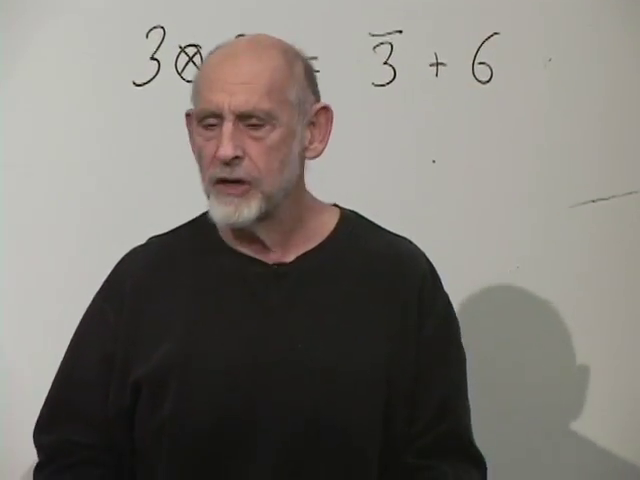
\includegraphics[width=0.68\textwidth]{lecture_04_figure_04.png}
\caption{Tích của hai quark tách thành một anti-triplet và một sextet.}
\lectureframe{00:39:33}
\end{figure}

Anti-triplet có thể được biểu diễn tường minh bằng cách co hai chỉ số quark với tensor epsilon bất biến,
\begin{equation}
(qq)^k_{\bar 3}
=\frac{1}{\sqrt2}\epsilon^{kij}q_iq_j.
\end{equation}
Đối tượng này có ba thành phần và biến đổi như một phản quark. Sáu tổ hợp đối xứng tạo thành sextet. Mệnh đề ở đây không phải là hai quark trở thành một phản quark theo nghĩa động lực học; mà là một sector của hàm sóng màu của chúng có cùng quy luật biến đổi như một phản quark.

\subsection{Một quark và một phản quark: \texorpdfstring{\(\boldsymbol 3\otimes\bar{\boldsymbol 3}\)}{3 x phản-3}}

Một trạng thái màu quark--phản quark có thể được xem như một ma trận \(3\times3\) \(M_i{}^j=q_i\bar q^j\). Mọi ma trận như vậy tách duy nhất thành phần vết và phần không vết của nó,
\begin{equation}
M=\frac{\operatorname{tr}M}{3}\boldsymbol 1
+\left(M-\frac{\operatorname{tr}M}{3}\boldsymbol 1\right).
\end{equation}
Vết là một thành phần bất biến đơn, còn phần không vết có tám thành phần. Do đó
\begin{equation}
\boldsymbol 3\otimes\bar{\boldsymbol 3}
=\boldsymbol 1\oplus\boldsymbol 8.
\label{eq:l4-three-times-threebar}
\end{equation}
Bỏ qua chuẩn hóa, singlet là
\begin{equation}
\ket{1}_{q\bar q}
=\frac{1}{\sqrt3}
(\ket{r\bar r}+\ket{g\bar g}+\ket{b\bar b}).
\end{equation}
Nó không thể biến đổi thành bất cứ tổ hợp nào khác vì nó là bất biến. Tám tổ hợp tuyến tính còn lại trộn lẫn với nhau. Chúng tạo thành biểu diễn adjoint, cũng là biểu diễn mà tám bộ sinh biến đổi theo.

\subsection{Ba quark}

Kết hợp thêm một quark thứ ba với phương trình~\eqref{eq:l4-three-times-three}. Nhánh phản bộ ba cho
\begin{equation}
\bar{\boldsymbol 3}\otimes\boldsymbol 3
=\boldsymbol 1\oplus\boldsymbol 8,
\end{equation}
nên tích ba quark chứa một singlet. Viết đầy đủ,
\begin{equation}
\boldsymbol 3\otimes\boldsymbol 3\otimes\boldsymbol 3
=\boldsymbol 1\oplus\boldsymbol 8\oplus\boldsymbol 8
\oplus\boldsymbol{10}.
\label{eq:l4-three-quark-full}
\end{equation}
Singlet màu là tổ hợp đỏ--xanh lục--xanh lam phản đối xứng hoàn toàn,
\begin{equation}
\ket{1}_{qqq}
=\frac{1}{\sqrt6}\epsilon^{ijk}\ket{q_iq_jq_k}.
\label{eq:l4-baryon-singlet}
\end{equation}
Vì \(\epsilon^{ijk}\) triệt tiêu bất cứ khi nào hai chỉ số trùng nhau, nên mọi số hạng khác không đều chứa một quark đỏ, một quark xanh lục và một quark xanh lam, với dấu luân phiên khi hoán đổi.

\begin{classroomqa}
\audiencequestion{Có phải các tổ hợp không singlet chỉ đơn thuần ít có khả năng xảy ra, nên có thể bỏ qua xác suất của chúng không?
\lecturetimestamp{00:46:02}}
\lecturerresponse{Không. Vấn đề là năng lượng, không phải xác suất nhỏ. Một trạng thái không singlet cô lập sẽ mang một trường màu ra tới khoảng cách lớn tùy ý và, trong chế độ giam hãm, sẽ đòi hỏi năng lượng không bị chặn trên. Động lực học đứng sau phát biểu đó sẽ được triển khai ở dưới.}
\end{classroomqa}

\subsection{Octet gluon}

Trường gluon biến đổi như octet trong Phương trình~\eqref{eq:l4-three-times-threebar}. Xét theo màu, nó mang một chỉ số triplet và một chỉ số anti-triplet, với phần vết singlet đã bị loại bỏ. Về mặt sơ đồ,
\begin{equation}
q\sim\boldsymbol 3,
\qquad
\bar q\sim\bar{\boldsymbol 3},
\qquad
G\sim\boldsymbol 8.
\end{equation}
Các ký hiệu này gọi tên các quy luật biến đổi; các hạt không theo nghĩa đen bằng các số nguyên 3 và 8.

Tổ hợp màu quark--phản quark thứ chín, tỉ lệ với ma trận đơn vị, là một singlet và không trộn với octet. Vì thế việc bỏ nó đi là nhất quán về mặt toán học: một trường gauge \(SU(3)\) là không vết và có tám thành phần thay vì chín thành phần của một trường gauge \(U(3)\).

\begin{classroomqa}
\audiencequestion{Vì sao tự nhiên bỏ đi gluon singlet phụ đó?
\lecturetimestamp{00:49:00}}
\lecturerresponse{Câu trả lời trực tiếp từ lý thuyết nhóm là singlet là một sector bất biến tách biệt, nên octet tự khép kín một cách nhất quán mà không cần đến nó. Lý do sâu hơn để chọn \(SU(3)\) thay vì \(U(3)\) không được suy ra ở đây; đó là một phần của cấu trúc gauge được suy ra từ hiện tượng học QCD.}
\end{classroomqa}

\section{Singlet màu dưới dạng hadron}

Các hạt tự do có khối lượng hữu hạn của tương tác mạnh là các singlet màu. Điều này không có nghĩa là quark hay gluon không có thực; nó có nghĩa là chúng không xuất hiện như các hạt tiệm cận cô lập. Các mô thức cơ bản để xây dựng singlet là
\begin{equation}
qqq,
\qquad
q\bar q,
\qquad
GG\ \text{and higher gluonic products}.
\end{equation}
Chúng lần lượt dẫn tới baryon, meson và glueball. Tích của vài đối tượng vốn đã không màu dĩ nhiên lại không màu, nên có thể xây dựng các trạng thái đa-hadron phức tạp hơn từ những thành phần này.

\begin{classroomqa}
\audiencequestion{Các singlet ba quark và quark--phản quark được gọi là gì, và gluon cũng có thể tạo thành singlet không?
\lecturetimestamp{00:51:38}}
\lecturerresponse{Một singlet ba quark là một baryon; một singlet quark--phản quark là một meson. Gluon cũng có thể kết hợp thành các singlet màu. Những trạng thái tương tác mạnh đơn giản nhất như vậy được gọi là glueball, và có thể có hơn hai gluon tham gia.}
\end{classroomqa}

Ba quark spin một phần hai luôn kết hợp thành một spin tổng thể bán nguyên, mặc dù mômen góc quỹ đạo có thể làm thay đổi giá trị bán nguyên nào xuất hiện. Meson quark--phản quark có spin nguyên. Glueball thuần gluon cũng có spin nguyên.

Đối với hai gluon, mệnh đề đầu tiên trên bảng chỉ là một phép đếm,
\begin{equation}
8\times8=1+63.
\end{equation}
Tổng cộng có 64 trạng thái màu; một tổ hợp là singlet và 63 tổ hợp còn lại thuộc các sector không singlet.

\begin{figure}[htbp]
\centering
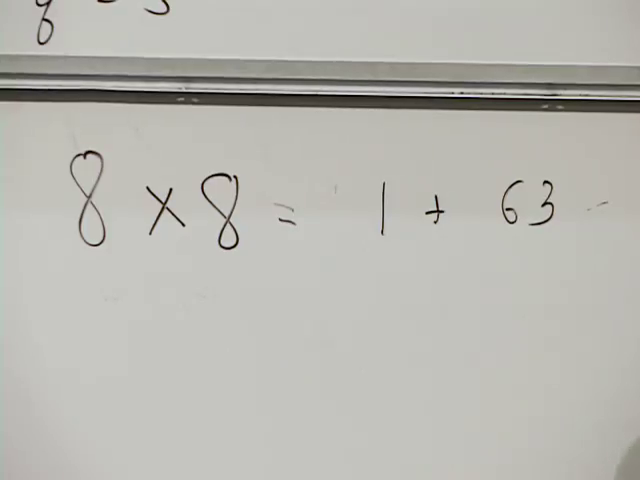
\includegraphics[width=0.68\textwidth]{lecture_04_figure_05.png}
\caption{Phép đếm trạng thái hai-gluon trên bảng: một singlet trong số 64 trạng thái.}
\lectureframe{00:53:44}
\end{figure}

Phân rã bất khả quy đầy đủ là
\begin{equation}
\boldsymbol 8\otimes\boldsymbol 8
=\boldsymbol 1\oplus\boldsymbol 8_S\oplus\boldsymbol 8_A
\oplus\boldsymbol{10}\oplus\overline{\boldsymbol{10}}
\oplus\boldsymbol{27}.
\label{eq:l4-eight-times-eight}
\end{equation}
Các số chiều cộng lại đúng:
\begin{equation}
1+8+8+10+10+27=64.
\end{equation}
Hai octet là những không gian con bất biến khác nhau, một đối xứng và một phản đối xứng dưới phép trao đổi hai thừa số adjoint. Singlet là kênh màu hai-gluon mà từ đó có thể tạo thành một trạng thái glueball.
\editorialnote{Trên bảng lúc đầu chỉ có \(8\times8=1+63\). Phần trao đổi sau đó trên lớp bổ sung các số chiều bất khả quy được liệt kê; các gạch trên và nhãn đối xứng được phục hồi ở đây theo ký hiệu \(SU(3)\) chuẩn.}

\subsection{Vì sao các điện tích quan sát được là số nguyên}

Điện tích của quark có hai loại,
\begin{equation}
Q_{\mathrm{up\text{-}like}}=+\frac23,
\qquad
Q_{\mathrm{down\text{-}like}}=-\frac13.
\end{equation}
Vì vậy ba quark có tổng điện tích nguyên: \(-1,0,+1,\text{ or }+2\),
tùy theo có bao nhiêu quark kiểu up. Tương tự, một quark và một phản quark có điện tích \(0\) hoặc \(\pm1\). Gluon không mang điện tích. Vì thế các singlet màu cơ bản được xây từ các biểu diễn quark quan sát được có điện tích nguyên, dù các thành phần của chúng mang điện tích phân số.

\begin{classroomqa}
\audiencequestion{Điện tích của quark lạ là bao nhiêu?
\lecturetimestamp{00:56:08}}
\lecturerresponse{Nó thuộc kiểu down, nên điện tích là \(-1/3\). Ba họ lặp lại cùng một mẫu điện tích: \((u,d)\), \((c,s)\) và \((t,b)\), với các điện tích \(+2/3\) và \(-1/3\) trong mỗi cặp.}
\end{classroomqa}

Tính singlet màu và điện tích nguyên liên hệ chặt chẽ với nhau đối với thành phần hạt này, nhưng chúng không phải là cùng một mệnh đề toán học. Tính nguyên ấy cũng dựa vào đúng các gán điện tích của Mô hình Chuẩn vừa được viết ra.

\begin{classroomqa}
\audiencequestion{Một singlet màu có phải là một trạng thái vướng víu không, và điều đó có cùng ý nghĩa như một cặp vướng víu trong một thí nghiệm Bell không?
\lecturetimestamp{00:56:58}}
\lecturerresponse{Hàm sóng màu singlet chắc chắn là vướng víu: nó là một chồng chập kết hợp, không phải tích của các màu riêng rẽ xác định. Về nguyên tắc các thành phần của nó có thể bị tách ra, nhưng sự giam hãm làm cho việc tách đó ngày càng tốn năng lượng và cuối cùng tạo ra các hadron mới. Vì thế đây không phải là một hệ thuận tiện cho thao tác kiểu Bell, dù trạng thái ấy là vướng víu.}
\end{classroomqa}

\section{Ý nghĩa của các phương trình tích tensor}

Đến đây, các bảng nhân xứng đáng được giải thích cụ thể hơn. Gọi \(\psi_i\) và \(\phi_j\) là các toán tử tạo ra hai đối tượng spin một phần hai; chúng có thể mô tả hai loại hạt, chẳng hạn một electron và một proton, hoặc hai bản sao của cùng một loại khi đã tính đến thống kê thích hợp. Mỗi chỉ số nhận hai giá trị. Bốn tích
\begin{equation}
\psi_\uparrow\phi_\uparrow,
\quad
\psi_\uparrow\phi_\downarrow,
\quad
\psi_\downarrow\phi_\uparrow,
\quad
\psi_\downarrow\phi_\downarrow
\end{equation}
sinh ra không gian tích tensor.

Nếu một phần tử nhóm tác dụng như \(U\) lên mỗi thừa số, thì nó tác dụng như \(U\otimes U\) lên tích. Theo thành phần,
\begin{equation}
\psi_i\phi_j
\longmapsto
U_i{}^kU_j{}^\ell\psi_k\phi_\ell.
\label{eq:l4-product-action}
\end{equation}
Đây là một biểu diễn bốn chiều, nhưng nó khả quy. Tổ hợp phản đối xứng
\begin{equation}
\frac{1}{\sqrt2}
(\psi_\uparrow\phi_\downarrow
-\psi_\downarrow\phi_\uparrow)
\end{equation}
được ánh xạ vào chính nó, còn ba tổ hợp đối xứng thì trộn lẫn với nhau. Trong cơ sở thích hợp với các tổ hợp đó, mọi ma trận của biểu diễn tích đều có dạng khối chéo,
\begin{equation}
D_{2\otimes2}(g)
\sim
\begin{pmatrix}
1&0\\
0&D_3(g)
\end{pmatrix}.
\label{eq:l4-spin-block-diagonal}
\end{equation}

\begin{classroomqa}
\audiencequestion{Một phương trình như \(\boldsymbol 3\otimes\boldsymbol 3=\bar{\boldsymbol 3}\oplus\boldsymbol 6\) biểu diễn thao tác nào?
\lecturetimestamp{00:57:51}}
\lecturerresponse{Vế trái tạo thành không gian trạng thái hợp thành. Nhóm tác dụng lên cả hai thừa số và vì thế trộn các trạng thái cơ sở của tích. Vế phải nói rằng một phép đổi cơ sở tách các trạng thái đó thành các tập bất biến: ba tổ hợp phản đối xứng biến đổi như một anti-triplet và sáu tổ hợp đối xứng biến đổi như một sextet. Dấu cộng có nghĩa là tổng trực tiếp của các phần, không phải phép cộng số học thông thường.}
\end{classroomqa}

\begin{classroomqa}
\audiencequestion{Làm sao ta biết 9 trạng thái tách thành \(3+6\), hay \(1+8\), thay vì, chẳng hạn, \(2+7\)?
\lecturetimestamp{01:04:39}}
\lecturerresponse{Chỉ đếm số chiều thì không thể quyết định cách tách. Ta phải biết \(SU(3)\) có những biểu diễn bất khả quy nào và xây dựng các không gian con bất biến, chẳng hạn bằng cách đối xứng hóa các chỉ số, phản đối xứng hóa chúng, hoặc tách phần vết khỏi phần không vết. Một sự phân loại đầy đủ đòi hỏi nhiều lý thuyết nhóm hơn; ở đây ta chỉ dùng các biểu diễn cần cho quark và gluon.}
\end{classroomqa}

Tensor epsilon bất biến làm cho việc xây dựng singlet trở nên minh bạch. Với \(SU(2)\),
\begin{equation}
\epsilon_{ij}U^i{}_kU^j{}_\ell
=(\det U)\epsilon_{k\ell}
=\epsilon_{k\ell}.
\end{equation}
Vì thế \(\epsilon_{ij}\psi^i\phi^j\) là bất biến. Với \(SU(3)\), phiên bản ba chỉ số cho
\begin{equation}
\epsilon_{ijk}U^i{}_aU^j{}_bU^k{}_c
=(\det U)\epsilon_{abc}
=\epsilon_{abc},
\end{equation}
điều này chứng minh tính bất biến của trạng thái ba-quark trong Phương trình~\eqref{eq:l4-baryon-singlet}.

\begin{classroomqa}
\audiencequestion{Có thể chỉ ra tường minh vì sao singlet không biến đổi không?
\lecturetimestamp{01:07:18}}
\lecturerresponse{Có. Hãy co tất cả các chỉ số cơ bản với tensor epsilon phản đối xứng hoàn toàn. Dưới phép biến đổi, tích các ma trận nhân epsilon với \(\det U\). Đối với một ma trận unita đặc biệt, định thức đó bằng 1, nên trạng thái đã co không đổi. Trong \(SU(2)\) điều này chứng minh singlet hai-spin; trong \(SU(3)\) nó chứng minh singlet ba-quark đỏ--lục--lam.}
\end{classroomqa}

\begin{classroomqa}
\audiencequestion{Phân rã đầy đủ của hai octet gluon là gì?
\lecturetimestamp{01:09:24}}
\lecturerresponse{Đó là phân rã trong Phương trình~\eqref{eq:l4-eight-times-eight}: một singlet, hai octet, một decuplet, một anti-decuplet và một biểu diễn 27 chiều. Có đúng một tổ hợp singlet màu của hai chỉ số octet.}
\end{classroomqa}

\begin{classroomqa}
\audiencequestion{Phân rã đầy đủ tương ứng đối với ba quark là gì?
\lecturetimestamp{01:11:51}}
\lecturerresponse{Câu trả lời cốt yếu về mặt vật lý là nó chứa một singlet. Hoàn tất phép cộng cho ta Phương trình~\eqref{eq:l4-three-quark-full}: một singlet, hai octet và một decuplet, tổng cộng \(1+8+8+10=27\) trạng thái.\editorialnote{Trong phần trao đổi này, giảng viên không nhớ phân rã đầy đủ của \(3\otimes3\otimes3\). Phần hoàn chỉnh chuẩn được cung cấp tường minh ở đây và được gắn nhãn tại đây thay vì quy cho câu trả lời bằng lời.}}
\end{classroomqa}

Ý tưởng tương tự mở rộng lên không gian hai gluon. Trong cơ sở tích tensor ngây thơ, \(SU(3)\) tác dụng thông qua các ma trận \(64\times64\). Trong một cơ sở thích nghi với các thành phần bất khả quy, các ma trận đó có dạng chéo khối,
\begin{equation}
\begin{aligned}
D_{8\otimes8}(g)
&\sim
\operatorname{diag}\bigl(
1,D_{8_S}(g),D_{8_A}(g),
\\
&\hspace{4.8em}
D_{10}(g),D_{\overline{10}}(g),D_{27}(g)
\bigr).
\end{aligned}
\end{equation}
Không có khối nào trộn với khối khác, mặc dù các trạng thái bên trong từng khối thì trộn lẫn với nhau.

\begin{classroomqa}
\audiencequestion{Phân rã tích tensor có phải chỉ là việc đổi sang một cơ sở trong đó ma trận biểu diễn lớn trở thành chéo khối không?
\lecturetimestamp{01:12:02}}
\lecturerresponse{Chính xác. Với hai spin, ma trận 4 chiều trở thành một khối singlet 1 chiều và một khối triplet 3 chiều. Với hai gluon, ma trận 64 chiều trở thành các khối có kích thước \(1,8,8,10,10,\text{ and }27\). Mỗi khối đều khép kín dưới mọi phép biến đổi nhóm.}
\end{classroomqa}

\begin{classroomqa}
\audiencequestion{Có tên gọi nào cho một trong những phần khép kín đó bên trong toàn bộ không gian tích tensor không?
\lecturetimestamp{01:14:55}}
\lecturerresponse{Đó là một không gian con bất biến mang một biểu diễn con. Khi không thể phân rã thêm nữa, nó mang một biểu diễn bất khả quy, hay irrep. Toàn bộ tích tensor là tổng trực tiếp của các thành phần bất khả quy đó.\editorialnote{Nguồn để ngỏ thuật ngữ được hỏi trong lớp. Trong câu trả lời, thuật ngữ chuẩn của lý thuyết biểu diễn được bổ sung.}}
\end{classroomqa}

\begin{classroomqa}
\audiencequestion{Khi các biểu diễn mười chiều không phải singlet và các biểu diễn khác bị gọi là không tồn tại, điều đó có nghĩa là phải hoàn toàn bỏ qua chúng hay không?\lecturetimestamp{01:15:36}}
\lecturerresponse{Chúng là những sector màu hợp lệ và có vai trò trong các phép tính trung gian, nhưng chúng không xuất hiện như những hạt cô lập có năng lượng hữu hạn trong phòng thí nghiệm. Chính sự giam hãm, chứ không phải sự thất bại của lý thuyết biểu diễn, ngăn chúng trở thành các trạng thái tiệm cận tự do.}
\end{classroomqa}

\section{Từ ý tưởng màu của Nambu đến sự giam hãm}

Ý tưởng về màu có trước công thức hóa cuối cùng của QCD. Ngay từ đầu những năm 1960, Yoichiro Nambu đã hiểu rằng một số lượng tử 3 giá trị ẩn có thể giải quyết một vấn đề nổi bật: quark mang điện tích phân số, nhưng không quan sát thấy hạt tự do nào mang điện tích phân số. Nếu các trạng thái vật lý bị buộc phải là singlet màu, thì quark xuất hiện trong các tổ hợp có điện tích nguyên như đã mô tả ở trên. Câu hỏi còn lại là câu hỏi động lực học: điều gì buộc mọi trạng thái tự do có năng lượng hữu hạn phải là singlet?

Bắt đầu với phép tương tự điện từ. Một điện tích và một điện tích trái dấu hút nhau. Đưa chúng lại gần nhau làm giảm năng lượng; còn ép các điện tích cùng dấu lại gần nhau thì cần thực hiện công. Bản thân trường chứa năng lượng dương,
\begin{equation}
E_{\mathrm{field}}
=\frac12\int d^3x\,\boldsymbol E^2
\end{equation}
trong các đơn vị tĩnh điện đơn giản. Một điện tích thuần để lại trường kéo dài rất xa ra ngoài hệ, trong khi một cặp trung hòa liên kết chặt chỉ có trường lưỡng cực tầm ngắn. Vì vậy, sự trung hòa loại bỏ năng lượng trường khỏi vùng bên ngoài.

Hãy tưởng tượng tăng độ ghép điện từ lên cực lớn. Mức phạt năng lượng trường đối với điện tích thuần sẽ trở nên lớn đến mức các đối tượng năng lượng thấp gần như đều trung hòa, và việc tách một thành phần mang điện ra có thể trở nên đòi hỏi năng lượng đến mức không khả thi. Nambu chuyển trực giác này sang màu: 8 điện tích màu là các nguồn của 8 trường gluon, nên năng lượng lớn của trường màu có thể cấm các trạng thái không singlet cô lập.

Trực giác ấy về cơ bản là đúng, nhưng QCD chứa một đặc trưng mới có tính quyết định. Photon không mang điện tích, còn gluon thì mang màu. Photon không phải là nguồn của trường điện từ cổ điển, và các phương trình Maxwell là tuyến tính: hai sóng điện từ chồng chất và đi xuyên qua nhau. Một gluon biến đổi trong octet màu, nên các gluon là nguồn của nhau và tương tác với nhau. Ngay cả các phần khác nhau của cùng một trường gluon cũng tương tác. Vì vậy trường gauge phi Abel là phi tuyến.

\subsection{Các ống thông lượng và thế tuyến tính}

Ở khoảng cách lớn, tự tương tác gluon ngăn không cho thông lượng màu loe ra như một trường lưỡng cực điện thông thường. Thông lượng bị ép vào một ống nối một quark với một phản quark. Cường độ trường và diện tích tiết diện của một ống dài xấp xỉ cố định, nên ống đó chứa một năng lượng trên mỗi đơn vị chiều dài xấp xỉ không đổi. Nếu \(\sigma\) ký hiệu lực căng dây này, thì
\begin{equation}
V(R)\simeq\sigma R+\text{constant}
\qquad (R\ \text{large}).
\label{eq:l4-linear-potential}
\end{equation}

\begin{figure}[htbp]
\centering
\includegraphics[width=0.78\textwidth]{lecture_04_figure_06.png}
\caption{Thông lượng màu bị bó lại thành một ống dài giữa một quark và một phản quark.}
\lectureframe{01:31:35}
\end{figure}

Điều này mạnh hơn thế Coulomb, vốn có độ lớn giảm theo \(1/R\). Kéo các nguồn màu ra xa hơn không làm lực suy yếu mãi; nó làm ống dài ra và tiếp tục cộng thêm năng lượng. Một điện tích màu đơn độc trong một thể tích vô hạn sẽ đòi hỏi một ống kéo dài vô tận và vì thế cần năng lượng không bị chặn trên. Đó chính là nội dung cụ thể của việc nói rằng chỉ các singlet màu mới có các trạng thái tiệm cận có năng lượng hữu hạn.
\editorialnote{Kí hiệu lực căng dây và thế ở khoảng cách lớn được viết tường minh làm cho phát biểu của nguồn, rằng một ống thông lượng đồng đều mang năng lượng đồng đều trên mỗi đơn vị chiều dài, trở nên định lượng.}

\subsection{Đứt dây và các jet}

Giả sử một va chạm cứng đánh trúng một quark bên trong một meson. Quark bắt đầu đi ra xa, nhưng ống thông lượng kéo giãn phía sau nó. Nó có thể mất động năng rồi bị kéo trở lại. Thường hơn, một khi năng lượng trường tích trữ đủ lớn, chân không tạo ra một cặp quark--phản quark mới. Phản quark mới làm đầu mút cho thông lượng gắn với quark đang thoát ra, còn quark mới làm đầu mút cho thông lượng gắn với phản quark ban đầu. Một singlet bị kéo giãn trở thành hai singlet ngắn hơn,
\begin{equation}
(q\bar q)_{\mathrm{stretched}}
\longrightarrow
(q\bar q)+(q\bar q).
\label{eq:l4-string-breaking}
\end{equation}

\begin{figure}[htbp]
\centering
\includegraphics[width=0.78\textwidth]{lecture_04_figure_07.png}
\caption{Sự tạo cặp làm đứt một ống thông lượng bị kéo giãn thành hai ống thông lượng singlet màu.}
\lectureframe{01:34:52}
\end{figure}

\begin{classroomqa}
\audiencequestion{Nếu một quark bị đánh trúng có đủ năng lượng để tiếp tục kéo giãn ống, thì ngoài việc bị kéo trở lại còn có thể xảy ra điều gì khác?
\lecturetimestamp{01:33:50}}
\lecturerresponse{Ống có thể bị đứt do sự tạo cặp quark--phản quark. Năng lượng của nó trở thành khối lượng và động năng của cặp mới. Các đầu mút nối lại thành hai singlet, nên quá trình này tạo ra thêm các meson chứ không tạo ra một quark cô lập.}
\end{classroomqa}

Nếu một trong các parton đó vẫn mang động lượng lớn, quá trình lặp lại. Kết quả là một thác các hadron singlet màu được chuẩn trực quanh hướng parton ban đầu: một jet. Sự chuyển hóa các quark và gluon giàu năng lượng thành các hadron được gọi là hadron hóa. Đối tượng mang màu khởi phát được suy ra từ jet, chứ không bao giờ được quan sát riêng rẽ.

\begin{classroomqa}
\audiencequestion{Sự đứt dây chỉ tạo ra meson, hay các hadron khác cũng có thể xuất hiện trong jet?
\lecturetimestamp{01:35:20}}
\lecturerresponse{Các hadron khác chắc chắn cũng có thể xuất hiện. Yêu cầu duy nhất về màu là các đối tượng quan sát được ở trạng thái cuối phải là singlet. Meson là hình dung đơn giản nhất cho một lần đứt, nhưng baryon, phản baryon và các tổ hợp singlet phức tạp hơn cũng có thể được tạo ra.}
\end{classroomqa}

Ba quark có thể cho thông lượng của chúng kết thúc tại một nút singlet màu. Bức tranh ba nhánh là đối ứng động lực học của tensor epsilon phản đối xứng trong Phương trình~\eqref{eq:l4-baryon-singlet}: không có thông lượng màu thuần nào thoát ra khỏi toàn bộ baryon.

\begin{figure}[htbp]
\centering
\includegraphics[width=0.72\textwidth]{lecture_04_figure_08.png}
\caption{Một nút thông lượng màu ba nhánh cho baryon, ở bên dưới hình phác họa đứt dây của meson.}
\lectureframe{01:36:12}
\end{figure}

\section{Các trường gauge, điện tích bảo toàn và Mô hình Chuẩn}

Ở mức độ hiện tại, có thể nhận ra một lý thuyết gauge là một lý thuyết trong đó một điện tích bảo toàn đóng vai trò nguồn cho một trường kiểu photon. Điện tích điện là nguồn của trường điện từ; 8 điện tích màu là nguồn của 8 trường gluon. Công thức sâu hơn làm cho đối xứng trở thành cục bộ và đưa vào một liên kết so sánh các trạng thái nội tại tại các điểm không-thời gian lân cận, nhưng cấu trúc đó không cần cho bức tranh giam hãm được phát triển ở đây.
\editorialnote{Công thức đối xứng cục bộ là nghĩa sâu hơn chuẩn của lý thuyết gauge mà nguồn có nhắc tới nhưng cố ý hoãn lại.}

Đối xứng, điện tích bảo toàn và thông lượng liên hệ chặt chẽ với nhau. Nếu các đường sức chỉ có thể kết thúc trên các điện tích, thì một nguồn không thể đơn giản biến mất trong khi thông lượng của nó vẫn còn gắn vào không đâu cả. Toàn bộ phần trường ở xa của nó cũng không thể biến mất tức thời, vì các biến đổi của trường lan truyền theo nhân quả. Ở dạng cục bộ, cùng một vật lý được biểu diễn bằng một phương trình liên tục,
\begin{equation}
\frac{\partial\rho}{\partial t}
+\boldsymbol\nabla\cdot\boldsymbol j=0,
\end{equation}
phương trình này nói rằng điện tích chỉ có thể rời khỏi một miền bằng cách chảy qua biên của miền đó. Lập luận bằng đường sức là bức tranh hình học của định luật bảo toàn cục bộ ấy.

Giờ ta có thể đặt kết quả này vào bên trong Mô hình Chuẩn. Màu đóng góp 8 phần tử sinh của \(SU(3)\) và 8 trường gluon tương ứng. Sector Abel cung cấp 1 phần tử sinh và 1 trường gauge. Ba phần tử sinh nữa thuộc về một \(SU(2)\) bổ sung, chứ không phải mômen động lượng không gian thông thường. Trước khi phá vỡ đối xứng, cấu trúc gauge là
\begin{equation}
SU(3)_c\times SU(2)_L\times U(1)_Y,
\end{equation}
với \(8+3+1=12\) phần tử sinh. Nhiệm vụ tiếp theo là hiểu \(SU(2)\) điện-yếu, rồi đến trường Higgs và cách photon quan sát được, \(W^\pm\) và \(Z\) xuất hiện.
\editorialnote{Nguồn gộp photon với 8 gluon và mô tả thừa số còn lại là \(SU(2)\times U(1)\). Trong Mô hình Chuẩn chưa phá vỡ đối xứng, thừa số Abel là siêu điện tích \(U(1)_Y\); photon chỉ xuất hiện sau khi trộn điện-yếu.}

Chuỗi lập luận trung tâm nay đã hoàn tất. Các nhóm trừu tượng tác dụng thông qua các biểu diễn; các phần tử sinh vi phân là các điện tích bảo toàn; quark, phản quark và gluon nằm trong \(\boldsymbol 3\),
\(\bar{\boldsymbol 3}\), và \(\boldsymbol 8\); các tích tensor xác định các hadron singlet; và trường gluon phi tuyến biến việc chọn singlet thành hiện tượng vật lý của sự giam hãm.
\chapter{Trường chuẩn, các thang tương tác và các dòng yếu mang điện}

Điện động lực học lượng tử và sắc động lực học lượng tử trông rất khác nhau trong phòng thí nghiệm, nhưng cả hai đều là các lý thuyết chuẩn. Thực ra, gần như mọi tương tác trong Mô hình Chuẩn đều được tổ chức theo cách này. Từ \emph{gauge} mang một ý nghĩa sâu hơn liên quan đến đối xứng địa phương, nhưng ta có thể tạm hoãn bộ máy đó lại. Hiện tại ta cần một mô tả vật lý tối thiểu: một lý thuyết chuẩn chứa các trường kiểu Maxwell, các nguồn được bảo toàn, các phép biến đổi đối xứng, các boson chuẩn, và các quy tắc phát xạ và hấp thụ những boson đó.

\section{Lý thuyết Maxwell như nguyên mẫu}

\subsection{Trường và thế}

Trường điện từ có sáu thành phần: ba thành phần của điện trường và ba thành phần của từ trường. Cùng thông tin đó có thể được mã hóa, với một phần dư thừa, trong một thế bốn-vectơ
\begin{equation}
A_\mu=(A_0,\boldsymbol A),
\end{equation}
trong đó \(A_0\) là thế tĩnh điện và \(\boldsymbol A\) là thế vectơ không gian. Trong giới hạn tĩnh điện, điện trường được suy ra từ gradient không gian,
\begin{equation}
\boldsymbol E=-\boldsymbol\nabla A_0,
\qquad
\boldsymbol F=q\boldsymbol E,
\end{equation}
trong khi từ trường là
\begin{equation}
\boldsymbol B=\boldsymbol\nabla\times\boldsymbol A.
\end{equation}
Dấu trong phương trình thứ nhất phụ thuộc vào định nghĩa chuẩn của thế; phần thảo luận trên bảng chủ yếu quan tâm đến thực tế rằng các trường là các đạo hàm của thế.
\editorialnote{Đối với các trường phụ thuộc thời gian, hệ thức đầy đủ là
\(\boldsymbol E=-\boldsymbol\nabla A_0-\partial_t\boldsymbol A\). Bài giảng cố ý làm việc ở mức tĩnh điện đơn giản hơn tại đây.}

\begin{figure}[htbp]
\centering
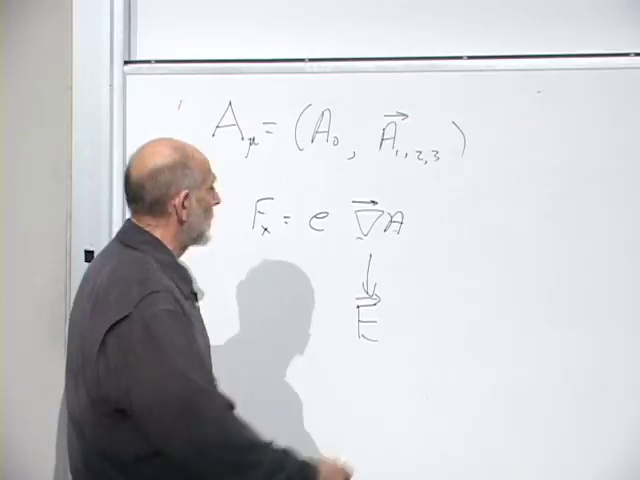
\includegraphics[width=0.62\textwidth]{lecture_05_figure_02.png}
\caption{Thế bốn điện từ và quan hệ đạo hàm của nó với trường.}
\lectureframe{00:03:33}
\end{figure}

Vì vậy điện động lực học chấp nhận hai mô tả tương đương: một theo \(\boldsymbol E\) và \(\boldsymbol B\), và một theo \(A_\mu\). Mô tả sau chỉ có bốn thành phần được viết ra vì những thế khác nhau có thể mô tả cùng một trường vật lý. Sự dư thừa đó là gợi ý đầu tiên ẩn sau từ gauge, dù ta chưa dùng nó một cách hình thức.

\subsection{Sóng và phân cực}

Các phương trình Maxwell cho phép các nghiệm sóng. Xét một sóng phẳng truyền theo một vectơ đơn vị \(\hat{\boldsymbol k}\). Tại mọi điểm, điện trường và từ trường đều là ngang:
\begin{equation}
\boldsymbol E\cdot\hat{\boldsymbol k}=0,
\qquad
\boldsymbol B\cdot\hat{\boldsymbol k}=0,
\qquad
\boldsymbol E\cdot\boldsymbol B=0.
\end{equation}
Trong các đơn vị với \(c=1\), độ lớn của chúng bằng nhau,
\begin{equation}
|\boldsymbol E|=|\boldsymbol B|.
\end{equation}
Đối với một sóng phân cực thẳng, hướng của \(\boldsymbol E\) xác định phân cực. Toàn bộ hình mẫu truyền đi với tốc độ ánh sáng.

Lượng tử hóa làm thay đổi ngôn ngữ nhưng không làm thay đổi cấu trúc phân cực. Một lượng tử của sóng điện từ là một photon. Việc vẽ photon như một điểm tất nhiên là dễ gây hiểu nhầm, nhưng vẫn hữu ích nếu hình dung rằng điểm đó mang một kim chỉ nhỏ theo phương ngang ghi lại phân cực của nó. Một tấm một phần tư bước sóng hoặc một phần tử quang học khác có thể làm quay phân cực đó. Tương tự, một trường Coulomb tĩnh cũng có thể được hình dung, dù chỉ rất gần đúng, như phát sinh từ sự phát xạ và hấp thụ lặp đi lặp lại của các photon.

\subsection{Nguồn, thông lượng và bảo toàn}

Sóng điện từ có thể lan truyền qua không gian rỗng, nhưng trường còn có các nguồn: điện tích và dòng điện. Một điện tích điểm dương tạo ra một điện trường xuyên tâm hướng ra ngoài tỉ lệ với \(1/r^2\). Số đường sức xuyên qua bất kỳ mặt cầu nào bao quanh điện tích là độc lập với bán kính của mặt cầu. Về mặt toán học,
\begin{equation}
\oint_{S^2}\boldsymbol E\cdot d\boldsymbol S
=\frac{Q_{\mathrm{enc}}}{\epsilon_0},
\label{eq:l5-gauss}
\end{equation}
trong hệ đơn vị SI.

Đây không chỉ là một cách thuận tiện để tính trường. Các đường sức điện chỉ có thể kết thúc trên điện tích. Nếu một điện tích cô lập đơn giản biến mất, thì trường của nó sẽ phải biến mất ở khắp nơi cùng lúc, vi phạm tính nhân quả, hoặc một mặt trước của phần trường bị thiếu sẽ phải lan truyền ra ngoài với các đường sức kết thúc trên không gian rỗng. Cả hai khả năng đều không được phép. Vì thế, hình học của thông lượng làm cho bảo toàn điện tích trở nên tự nhiên: điện tích có thể chuyển động, và các điện tích trái dấu có thể hủy nhau, nhưng điện tích thuần không thể biến mất cục bộ nếu không có một dòng bù.

Phát biểu cục bộ tương ứng là phương trình liên tục
\begin{equation}
\partial_t\rho+\boldsymbol\nabla\cdot\boldsymbol J=0.
\label{eq:l5-continuity}
\end{equation}
\editorialnote{Phương trình~\eqref{eq:l5-continuity} là dạng toán học cục bộ chuẩn của lập luận thông lượng nhân quả đã được triển khai bằng lời trong bài giảng.}

\subsection{Một định nghĩa làm việc về lý thuyết chuẩn}

Giờ đây ta có thể phát biểu mẫu hình thao tác. Một lý thuyết chuẩn có:
\begin{itemize}
\item các trường kiểu điện và kiểu từ;
\item các sóng mà, khi tương tác đủ yếu, trông giống sóng ánh sáng;
\item các nguồn tương tự điện tích;
\item một định luật Gauss gắn thông lượng với các nguồn đó;
\item một định luật bảo toàn và một đối xứng đi kèm;
\item các lượng tử của trường, được gọi là boson chuẩn; và
\item một hằng số liên kết chi phối sự phát xạ và hấp thụ.
\end{itemize}
Nguồn không nhất thiết phải là điện tích. Như một ví dụ cố ý phi vật lý, hãy tưởng tượng chuẩn hóa số baryon. Proton và neutron đều có số baryon \(+1\), nên chúng sẽ đẩy nhau thông qua một lực mới kiểu Coulomb; một proton và một phản proton sẽ hút nhau. Một lý thuyết như vậy có thể hình dung được về mặt toán học, nhưng tự nhiên không cung cấp trường chuẩn tầm xa quan sát được nào ghép với số baryon. Bảo toàn tự nó không bảo đảm có một lực chuẩn.

Điện tích điện quả thật đi kèm với một đối xứng. Đối với một trường vật chất mang điện,
\begin{equation}
\psi(x)\longmapsto e^{i\theta}\psi(x).
\label{eq:l5-u1}
\end{equation}
Đối xứng pha và bảo toàn điện tích là hai mặt của cùng một cấu trúc. Về sau ta có thể làm cho \(\theta\) phụ thuộc vào không-thời gian và thấy vì sao thế \(A_\mu\) là cần thiết. Ở đây phép biến đổi toàn cục là đủ để xác định điện tích được bảo toàn.

\section{QCD như ví dụ không Abel}

\subsection{Bộ ba, phản bộ ba và ma trận gluon}

Trong sắc động lực học lượng tử, một trường quark mang một chỉ số màu \(i\in\{r,g,b\}\) và biến đổi theo biểu diễn cơ bản của \(SU(3)\):
\begin{equation}
q'_i=U_{ij}q_j,
\qquad
U^\dagger U=\boldsymbol 1,
\qquad
\det U=1.
\label{eq:l5-q-transform}
\end{equation}
Đây là một phép quay trong không gian màu phức ba chiều, không phải một phép quay của không gian vị trí thông thường. Biểu diễn ba thành phần này cũng được gọi là biểu diễn định nghĩa.

Các trường phản hạt được biểu diễn bởi các biến liên hợp phức. Lấy liên hợp phức của Phương trình~\eqref{eq:l5-q-transform} cho ta
\begin{equation}
q_i^{\prime *}=U_{ij}^*q_j^*.
\label{eq:l5-antiquark-transform}
\end{equation}
Vì vậy quark biến đổi như \(\boldsymbol 3\), còn phản quark biến đổi như \(\bar{\boldsymbol 3}\).

\begin{figure}[htbp]
\centering
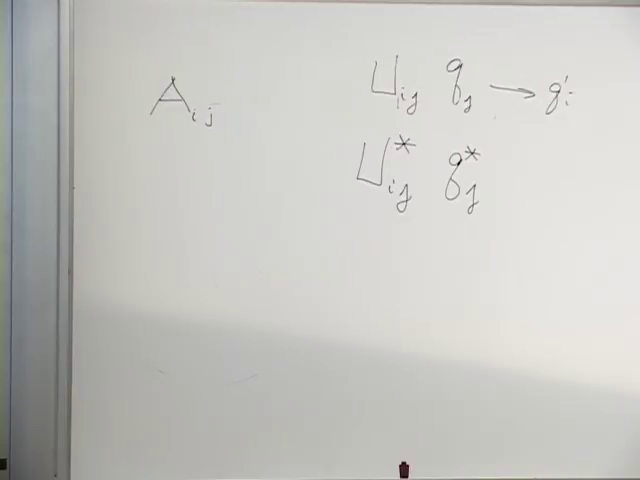
\includegraphics[width=0.62\textwidth]{lecture_05_figure_03.png}
\caption{Phép biến đổi cơ bản và phép biến đổi phản bộ ba liên hợp phức của nó.}
\lectureframe{00:18:47}
\end{figure}

\begin{classroomqa}
\audiencequestion{Có bao nhiêu ma trận \(U\) -- 7, 8 hay 9?
\lecturetimestamp{00:19:37}}
\lecturerresponse{Có vô hạn phần tử nhóm \(U\). Số hữu hạn đang được đếm là số các phần sinh độc lập, và với \(SU(3)\) thì số đó là 8. Một ma trận \(3\times3\) tổng quát có 9 ô ma trận, nhưng điều kiện unita đặc biệt chỉ để lại 8 hướng liên tục.}
\end{classroomqa}

Trường gluon có thể được viết thành một ma trận không vết \(A_{ij}\). Một chỉ số biến đổi như một quark và chỉ số kia như một phản quark, nên cấu trúc màu của nó là
\begin{equation}
\boldsymbol 3\otimes\bar{\boldsymbol 3}
=\boldsymbol 1\oplus\boldsymbol 8.
\end{equation}
QCD giữ lại bát tử không vết,
\begin{equation}
A_{ii}=\operatorname{tr}A=0,
\end{equation}
và loại bỏ đơn tử. Đó là lý do QCD có 8 gluon thay vì 9. Tổng quát hơn, \(SU(N)\) có
\begin{equation}
N^2-1
\end{equation}
phần sinh và cũng có từng ấy trường boson chuẩn.

Photon là trung hòa đối với \(U(1)\) điện: việc quay pha của một electron không biến photon thành một photon khác. Gluon thì khác. Một gluon mang một màu và một phản màu, nên nó biến đổi theo biểu diễn adjoint. Chẳng hạn, một tổ hợp đỏ--phản lam không phải là một đơn tử màu dù nó chứa một màu và một phản màu.

\subsection{Dòng chỉ số và tự tương tác}

Có thể đọc ra quy tắc tương tác bằng cách lần theo các chỉ số. Về mặt sơ đồ, một quark có màu \(i\) có thể trở thành một quark có màu \(j\) đồng thời phát ra một gluon mang dòng màu tương ứng:
\begin{equation}
q_i\longrightarrow q_j+A_{ij}.
\label{eq:l5-quark-gluon-vertex}
\end{equation}
Vị trí chính xác của \(i\) và \(j\) phụ thuộc vào quy ước mũi tên; nội dung bất biến là mọi chỉ số đi vào một đỉnh phải tiếp tục dọc theo một đường khác. Không có chỉ số màu nào bị mất.

Quy tắc này áp dụng trong mọi lý thuyết chuẩn \(SU(N)\). Vật chất cơ bản có một chỉ số, vật chất phản cơ bản có một chỉ số liên hợp, và một boson chuẩn có một chỉ số mỗi loại. Tên gọi vật lý có thể thay đổi, nhưng cấu trúc chỉ số thì giữ nguyên.

Bởi vì bản thân một gluon mang màu, nó có thể phát ra một gluon khác. Một gluon \(A_{ij}\) có thể tách qua một chỉ số trung gian \(k\), về mặt sơ đồ,
\begin{equation}
A_{ij}\longrightarrow A_{ik}+A_{kj}.
\label{eq:l5-three-gluon-index}
\end{equation}
Đây không phải là một đỉnh Yang--Mills hoàn chỉnh, nhưng nó biểu diễn dòng màu. Trong điện động lực học thông thường không có điều gì tương tự xảy ra với photon. Vì thế gluon tác dụng lực lên gluon, và động lực học của trường không Abel phức tạp hơn nhiều so với lý thuyết tuyến tính của Maxwell.

Một hệ quả định tính là giam hãm. Các đường thông lượng màu không thể kết thúc, và tự tương tác của chúng kéo chúng thành một ống nối một quark với một phản quark. Ống này mang một năng lượng gần như không đổi trên một đơn vị chiều dài:
\begin{equation}
V(R)\simeq \sigma R.
\end{equation}
Vì vậy, kéo hai đầu mút ra xa hơn sẽ tích trữ nhiều năng lượng hơn thay vì giải phóng màu cô lập. Đây là hình ảnh cục keo dẻo quánh: chính trường ngăn các thành phần mang màu thoát ra như các hạt tự do.

\section{Các hằng số liên kết và ý nghĩa của mạnh hay yếu}

\subsection{Điện tích như một biên độ phát xạ}

Một lý thuyết chuẩn vẫn cần một hằng số liên kết. Trong QED, điện tích electron \(e\) là hệ số gắn với một đỉnh electron--photon. Nó là một biên độ, còn xác suất là bình phương của các biên độ. Về mặt thao tác, hãy hình dung chặn đột ngột một electron nhanh trong một ống tia catôt. Xác suất phát ra một photon tỉ lệ với \(e^2\), với các hệ số quy ước được hấp thụ vào hằng số cấu trúc tinh tế,
\begin{equation}
\alpha=\frac{e^2}{4\pi\hbar c}
\simeq \frac{1}{137}.
\label{eq:l5-alpha}
\end{equation}
Trong các đơn vị tự nhiên \(\hbar=c=1\), hằng số liên kết là không thứ nguyên. Một mức cỡ 1 phần trăm cho một phát xạ sơ cấp làm cho điện từ học là yếu theo nghĩa nhiễu loạn: đa số electron bị dừng lại không phóng ra một chùm photon cứng.

\subsection{Đơn vị tự nhiên liên hệ năng lượng, thời gian và khoảng cách}

Đặt
\begin{equation}
c=1,
\qquad
\hbar=1.
\end{equation}
Khi đó thời gian và khoảng cách có cùng đơn vị, còn năng lượng có đơn vị nghịch đảo:
\begin{equation}
E=\hbar\omega\longrightarrow E=\omega\sim\frac1t,
\qquad
x\sim t\sim\frac1E.
\end{equation}
Năng lượng lớn thăm dò các khoảng cách ngắn và các thời gian ngắn.

Để định hướng,
\begin{equation}
1\ {\rm eV}^{-1}
=\frac{\hbar c}{1\ {\rm eV}}
\simeq 1.97\times10^{-7}\ {\rm m}.
\end{equation}
Vì vậy, một độ dài nguyên tử cỡ \(10^{-10}\ {\rm m}\) tương ứng xấp xỉ với một kiloelectronvolt nghịch đảo. Đây là các chuyển đổi bậc độ lớn, không phải quang phổ chính xác.

\subsection{Sự phân cấp bên trong một nguyên tử}

Đối với một nguyên tử điển hình, lấy
\begin{equation}
R_{\rm atom}\sim10^{-10}\ {\rm m}.
\end{equation}
Ánh sáng đi qua khoảng cách này trong
\begin{equation}
t_{\rm transit}^{\rm atom}\sim10^{-18}\ {\rm s}.
\end{equation}
Tuy nhiên, trong một nguyên tử nhẹ, electron chỉ chuyển động với một phần nhỏ của tốc độ ánh sáng. Trong bức tranh Bohr, \(v/c\sim\alpha\), nên một thời gian quỹ đạo điển hình dài hơn:
\begin{equation}
t_{\rm orbit}^{\rm atom}\sim10^{-16}\ {\rm s}.
\end{equation}

Một nguyên tử kích thích còn mất lâu hơn nữa để phát xạ:
\begin{equation}
t_{\rm decay}^{\rm atom}\sim10^{-9}\ {\rm s}
\end{equation}
như một ước lượng thô ở quy mô bài giảng. Có hai sự ức chế trong bức tranh vật lý. Lực điện từ chỉ tạo ra gia tốc vừa phải, và một electron đang gia tốc lại có thêm một xác suất phát xạ nhỏ khác do \(\alpha\) chi phối. Vì vậy hằng số cấu trúc tinh tế nhỏ tạo ra một sự phân cấp giữa các thời gian truyền qua, quỹ đạo và phân rã bức xạ.

\subsection{Sự vắng mặt của phân cấp trong một hadron}

Một hadron là một hệ liên kết kiểu nguyên tử được tạo bởi quark và gluon, nhưng thang kích thước của nó nhỏ hơn nhiều:
\begin{equation}
R_{\rm hadron}\sim10^{-15}\ {\rm m},
\qquad
t_{\rm transit}^{\rm hadron}\sim10^{-23}\ {\rm s}.
\end{equation}
Các quark đi ngang qua hadron trên về cơ bản cùng một thang thời gian, và các hadron kích thích phân rã mạnh cũng sống xấp xỉ
\begin{equation}
t_{\rm orbit}^{\rm hadron}
\sim t_{\rm decay}^{\rm hadron}
\sim10^{-23}\ {\rm s}.
\end{equation}
Một hadron bị va chạm có thể dao động và phát ra một pion gần như nhanh như tính nhân quả cho phép. Không có sự tách biệt 7 hoặc 9 bậc độ lớn như bên trong một nguyên tử.

\begin{classroomqa}
\audiencequestion{Thuyết tương đối hẹp có hàm ý rằng một hadron không thể phân rã nhanh hơn đáng kể so với thời gian ánh sáng đi ngang qua nó không?
\lecturetimestamp{00:47:15}}
\lecturerresponse{Đó là một cách hợp lý để phát biểu cận bậc độ lớn. Các phân rã mạnh xảy ra gần nhanh bằng mức mà kích thước của hệ cho phép; không có hằng số liên kết nhỏ hay sự ức chế lớn nào khác làm chậm chúng lại.}
\end{classroomqa}

Vì thế, hằng số ghép mạnh tương ứng lớn hơn \(\alpha\) rất nhiều. Ở một thang hadron dùng để minh họa, bài giảng nêu
\begin{equation}
\alpha_{\rm QCD}\sim0.2,
\end{equation}
gần với 1 hơn nhiều so với \(1/137\). Đây là nguồn gốc động lực học của tên gọi cũ \emph{các tương tác mạnh}.
\editorialnote{Hằng số ghép QCD chạy theo năng lượng, nên \(\alpha_s\) không phải là một con số cố định duy nhất. Giá trị được nêu ra là một giá trị minh họa phụ thuộc thang, đúng như chủ ý của bài giảng.}

\begin{classroomqa}
\audiencequestion{Bên tương tự của tương tác mạnh có được gọi đơn giản là hằng số lực mạnh không?
\lecturetimestamp{00:48:17}}
\lecturerresponse{Theo quy ước, nó được gọi là \(\alpha_{\rm QCD}\), hoặc thường hơn là \(\alpha_s\). Hằng số điện từ thường chỉ được gọi là \(\alpha\), mặc dù \(\alpha_{\rm QED}\) có thể được dùng khi cả hai cùng xuất hiện trong một cuộc thảo luận.}
\end{classroomqa}

\begin{classroomqa}
\audiencequestion{Trong một bài báo, người ta có phân biệt độ ghép điện từ trần với giá trị đo được, đã bị che chắn không?
\lecturetimestamp{00:48:38}}
\lecturerresponse{Có. Người ta nói về một độ ghép trần và một độ ghép tái chuẩn hóa. Phân cực chân không làm cho độ ghép hiệu dụng phụ thuộc vào thang mà tại đó nó được đo.}
\end{classroomqa}

\section{Điều bí ẩn của phân rã yếu}

Tương tác yếu được đặt tên từ thời gian phân rã rất dài của chúng. Chúng thường chậm hơn các phân rã mạnh và thậm chí có thể chậm hơn bức xạ nguyên tử. Ví dụ lâu đời nhất là phân rã beta hạt nhân.

\subsection{Phân rã beta của neutron}

Một neutron tự do phân rã theo
\begin{equation}
n\longrightarrow p+e^-+\bar\nu_e.
\label{eq:l5-neutron-decay-intro}
\end{equation}
Bài giảng dùng thời gian sống xấp xỉ 12 phút, dài đến khó tin so với \(10^{-23}\ {\rm s}\). Các giá trị chính xác hiện đại không quan trọng đối với lập luận này.

Một phần của sự chậm này là do động học. Xấp xỉ,
\begin{equation}
\begin{aligned}
m_n&\simeq940\ {\rm MeV},
&
m_p&\simeq939\ {\rm MeV},
\\
m_e&\simeq0.5\ {\rm MeV}.
\end{aligned}
\end{equation}
Chỉ một phần rất nhỏ năng lượng nghỉ của neutron khả dụng dưới dạng động năng. Nếu neutron nhẹ hơn tổng các khối lượng nghỉ cuối, phân rã sẽ là bất khả. Nếu nó chỉ nằm cao hơn ngưỡng một lượng vô cùng nhỏ, không gian pha khả dụng sẽ rất nhỏ và phân rã sẽ chậm. Nhưng chỉ riêng không gian pha không thể giải thích một thời gian sống được đo bằng phút.

\subsection{Pion tích điện loại bỏ lời biện hộ bằng ngưỡng}

Hãy xét thêm
\begin{equation}
\pi^-\longrightarrow e^-+\bar\nu_e
\end{equation}
và quá trình liên hợp điện tích của nó. Pion có năng lượng dư dả trên ngưỡng của kênh electron, vậy mà thời gian sống yếu của nó vẫn ở bậc nanôgiây chứ không phải bậc hadron \(10^{-23}\) giây. Một kênh tương tự với muon sẽ sớm trở nên quan trọng. Vì thế, điều bí ẩn là nội tại của tương tác yếu, chứ không chỉ là một hệ quả ngẫu nhiên của việc các khối lượng của neutron gần như suy biến.

\editorialnote{Thời gian sống của pion tích điện vào khoảng \(26\ {\rm ns}\), và kênh trội là \(\pi^-\to\mu^-\bar\nu_\mu\). Kênh electron bị ức chế helicity. Bài giảng trước hết dùng kênh electron vì việc theo dõi các hạt trong đó là đơn giản nhất, rồi quay lại kênh muon trội.}

Thuật ngữ phân rã beta có nguồn gốc lịch sử từ cách gọi các electron phát ra là tia beta. Các ví dụ pion và neutron liên quan đến cùng một tương tác dòng tích điện, dù động học của chúng khác nhau rất mạnh.

\section{Bảng các quark và lepton}

\subsection{Màu tác động theo chiều dọc}

Hãy sắp xếp sáu hương quark thành ba cột ghép cặp,
\begin{equation}
(u,d),\qquad(c,s),\qquad(t,b),
\end{equation}
và đặt một bản sao đỏ, lục và lam của mỗi quark vào các hàng riêng. Đối xứng màu \(SU(3)\) tác động theo chiều dọc: nó quay các phiên bản đỏ, lục và lam của quark up vào nhau, và đồng thời thực hiện cùng phép quay màu ấy trên down, charm, strange, top và bottom. Nó không biến một quark up thành một quark down.

\subsection{Isospin yếu tác động theo chiều ngang}

Đối xứng yếu tác động theo hướng kia. Nó trộn từng cặp lân cận
\begin{equation}
Q_1=\begin{pmatrix}u\\d\end{pmatrix},
\qquad
Q_2=\begin{pmatrix}c\\s\end{pmatrix},
\qquad
Q_3=\begin{pmatrix}t\\b\end{pmatrix}.
\label{eq:l5-quark-doublets}
\end{equation}
Các quark kiểu up có điện tích \(+2/3\), còn các quark kiểu down có điện tích \(-1/3\), nên điện tích thay đổi một đơn vị qua mỗi cặp.
\editorialnote{Nguồn tư liệu thoáng chốc nói rằng quark down có điện tích \(-2/3\). Phép trừ ở đoạn lân cận và mọi quá trình tiếp theo đều đòi hỏi giá trị chuẩn \(-1/3\), và ở đây dùng giá trị ấy.}

Vì đối xứng này tác động trên các doublet, nhóm tự nhiên là \(SU(2)\). Nó tác động lên mọi bản sao màu của mỗi doublet quark mà không làm đổi màu.

Còn có một hàng hạt thứ tư không mang điện tích màu và vì thế không tương tác với gluon: các lepton. Chúng tạo thành thêm ba doublet,
\begin{equation}
L_e=\begin{pmatrix}\nu_e\\e^-\end{pmatrix},
\qquad
L_\mu=\begin{pmatrix}\nu_\mu\\\mu^-\end{pmatrix},
\qquad
L_\tau=\begin{pmatrix}\nu_\tau\\\tau^-\end{pmatrix}.
\label{eq:l5-lepton-doublets}
\end{equation}
Các neutrino trung hòa điện; electron, muon và tau có điện tích \(-1\). Một lần nữa, hai thành viên khác nhau đúng một đơn vị điện tích. Electron, muon và tau có cùng các số lượng tử gauge nhưng khối lượng khác nhau, cũng như ba thế hệ quark kiểu up hay kiểu down lặp lại cùng một mẫu điện tích.

\begin{figure}[htbp]
\centering
\includegraphics[width=0.82\textwidth]{lecture_05_figure_05.png}
\caption{Bảng trên bảng đen: màu tác động giữa các hàng đỏ, lam và lục, còn \(SU(2)\) yếu nối các cột hương ghép đôi và hàng lepton.}
\lectureframe{01:03:35}
\end{figure}

Việc gọi lepton là màu thứ tư ở giai đoạn này chỉ là một phép loại suy. Chúng tạo thành hàng thứ tư trong bảng doublet yếu, nhưng \(SU(3)\) QCD thông thường không quay quark thành lepton.

\section{Xây dựng các boson yếu mang điện}

\subsection{Các số lượng tử của các boson mang điện}

Các boson gauge mang những tính chất biến đổi cần thiết để chuyển từ một thành viên của doublet sang thành viên kia. Hãy bắt đầu với cặp lepton
\(e^-\bar\nu_e\). Nó có điện tích \(-1\), nên boson gauge mang điện tương ứng được gọi là \(W^-\):
\begin{equation}
W^-\sim e^-\bar\nu_e.
\end{equation}
Cùng các số lượng tử ấy cũng xuất hiện từ một quark down và một phản quark up:
\begin{equation}
W^-\sim d\bar u.
\end{equation}
Ký hiệu \(\sim\) có nghĩa là có cùng các số lượng tử gauge liên quan như. Nó không có nghĩa rằng \(W\) theo nghĩa đen là một trạng thái liên kết của các hạt này. Phản hạt có các tổ hợp liên hợp,
\begin{equation}
W^+\sim e^+\nu_e\sim\bar d u.
\end{equation}

Các đỉnh yếu mang điện bao gồm
\begin{align}
e^-&\longrightarrow\nu_e+W^-,
&
\mu^-&\longrightarrow\nu_\mu+W^-,
\label{eq:l5-lepton-w}\\
d&\longrightarrow u+W^-,
&
s&\longrightarrow c+W^-,
\label{eq:l5-quark-w}
\end{align}
cùng với các chuyển tiếp tương tự cho thế hệ thứ ba khi được phép về mặt động học. Boson gauge thực hiện về mặt động lực cùng sự trộn theo chiều ngang mà đối xứng thực hiện trên doublet.

\begin{classroomqa}
\audiencequestion{Bảo toàn điện tích buộc boson phát ra phải có điện tích \(-1\), nhưng tại sao các chuyển tiếp của electron, quark down và quark strange đều phải liên quan đến cùng một hạt?
\lecturetimestamp{01:12:56}}
\lecturerresponse{Đó là một sự kiện thực nghiệm được mã hóa trong đối xứng yếu chung. Tự nhiên hoàn toàn có thể một cách nhất quán đã gán một boson kiểu \(W\) khác nhau cho mỗi họ, hoặc riêng cho quark và lepton. Thay vào đó, một \(SU(2)\) duy nhất tác động đồng thời lên mọi doublet, và cùng các boson gauge mang điện ấy làm trung gian cho mọi chuyển tiếp này.}
\end{classroomqa}

\subsection{Đọc và đảo một đỉnh}

Một đỉnh đơn lẻ biểu diễn cả một họ quá trình. Đảo một đường đi vào thành một đường đi ra sẽ biến một hạt thành phản hạt của nó, và đảo một đường \(W^-\) sẽ cho một \(W^+\). Vì thế, ta có thể đọc một đỉnh như sự phát xạ, hấp thụ, phân rã, hủy cặp, hoặc phản ứng nghịch, miễn là điện tích, động lượng và mọi số lượng tử liên quan đều được theo đúng một cách nhất quán.

\begin{classroomqa}
\audiencequestion{Các mũi tên và các đường trong những đỉnh yếu này có thể bị đảo được không?
\lecturetimestamp{01:14:51}}
\lecturerresponse{Có. Một đường có thể được chuyển từ trạng thái cuối sang trạng thái đầu hoặc ngược lại, nhưng khi đó một hạt sẽ trở thành phản hạt của nó. Do đó cùng một đỉnh cục bộ mô tả nhiều phản ứng với định hướng khác nhau.}
\end{classroomqa}

\begin{classroomqa}
\audiencequestion{Việc viết một \(W^-\) với các đường strange và charm có nghĩa là boson ấy theo nghĩa đen là một quark strange liên kết với một phản quark charm không?
\lecturetimestamp{01:15:43}}
\lecturerresponse{Không. Việc theo dõi các đường chỉ nói rằng \(W^-\) mang sự thay đổi số lượng tử giữa các cột ấy. Nếu giản đồ được đọc như một phân rã, một \(W^-\) đủ năng lượng có thể tạo ra một quark strange và một phản quark charm; nó không được cấu tạo từ chúng.}
\end{classroomqa}

\begin{classroomqa}
\audiencequestion{Một electron và một phản neutrino có thể tạo ra một \(W\), rồi hạt đó sinh ra một cặp quark không?
\lecturetimestamp{01:17:22}}
\lecturerresponse{Chính xác. Nếu có đủ năng lượng trong hệ quy chiếu khối tâm, các lepton ban đầu có thể tạo thành trạng thái trung gian dòng tích điện, và trạng thái ấy có thể đi ra qua một kênh quark được phép. Hai đỉnh đó chính là những đỉnh dùng trong phân rã, chỉ được đọc theo một định hướng khác.}
\end{classroomqa}

\subsection{Boson thứ ba còn thiếu}

Một nhóm \(SU(2)\) có ba bộ sinh, nên có ba trường gauge. Cho đến nay ta mới chỉ hiển thị \(W^+\) và \(W^-\). Một trường thứ ba, trung hòa điện, phải gắn với những tổ hợp đường chéo như các số lượng tử electron--positron và neutrino--phản neutrino. Nó được cố ý để lại lẩn khuất trong nền. Quan hệ của nó với boson vật lý \(Z\) và photon đòi hỏi sự trộn điện-yếu, điều này sẽ đến sau.

\begin{classroomqa}
\audiencequestion{Lực yếu và lực mạnh đã được nghi ngờ ở những thời điểm lịch sử khác nhau sao?
\lecturetimestamp{01:24:11}}
\lecturerresponse{Các gốc rễ thực nghiệm của chúng xuất hiện cùng nhau trong giai đoạn đầu của hiện tượng phóng xạ. Phân rã alpha hé lộ vật lý hạt nhân và tương tác mạnh, phân rã beta hé lộ tương tác yếu, còn phân rã gamma phát ra các photon điện từ. Ngay từ thời Becquerel đã có đủ cả ba đầu mối, rất lâu trước khi các lý thuyết trường hiện đại của chúng tồn tại.}
\end{classroomqa}

\section{Các ví dụ đã giải về phân rã dòng tích điện}

\subsection{Phân rã pion}

Pion mang điện âm có thành phần quark hóa trị
\begin{equation}
\pi^-=d\bar u.
\end{equation}
Các số lượng tử ấy có thể hủy thành một \(W^-\), rồi hạt đó có thể sinh ra một lepton mang điện và phản neutrino tương ứng:
\begin{align}
\pi^-&\longrightarrow W^{-*}
\longrightarrow e^-+\bar\nu_e,
\label{eq:l5-pion-electron}\\
\pi^-&\longrightarrow W^{-*}
\longrightarrow \mu^-+\bar\nu_\mu.
\label{eq:l5-pion-muon}
\end{align}
Dấu sao nhắc ta rằng \(W\) trung gian là ảo. Kênh thứ hai là kênh trội.

\begin{figure}[htbp]
\centering
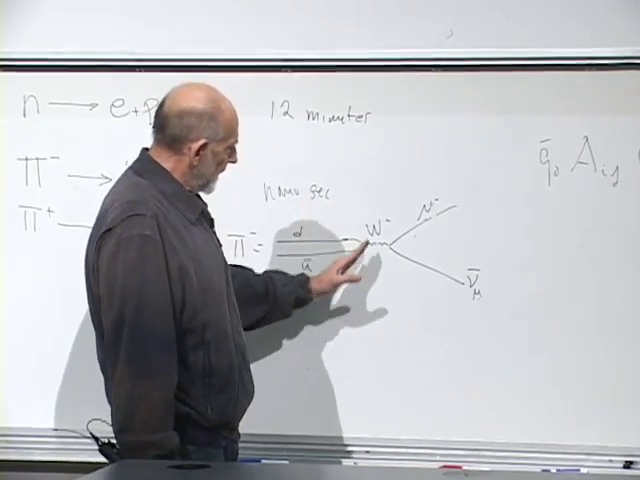
\includegraphics[width=0.72\textwidth]{lecture_05_figure_04.png}
\caption{Một pion \(d\bar u\) hủy thành một \(W^-\) ảo, rồi thành một lepton mang điện và phản neutrino tương ứng của nó.}
\lectureframe{01:19:38}
\end{figure}

\begin{classroomqa}
\audiencequestion{Đây có thực sự là một giản đồ Feynman không, mặc dù chiều thời gian được vẽ theo phương ngang chứ không phải phương thẳng đứng?
\lecturetimestamp{01:20:21}}
\lecturerresponse{Có. Hướng của thời gian trên trang là một quy ước. Một khi một hướng đã được tuyên bố là thời gian và mọi mũi tên đều được diễn giải nhất quán, hình vẽ mang cùng thông tin tương tác.}
\end{classroomqa}

\begin{classroomqa}
\audiencequestion{Có thể hiểu sơ đồ này giống một phản ứng hóa học thuận nghịch hơn là một sự phân rã một chiều không thể đảo ngược không?
\lecturetimestamp{01:21:35}}
\lecturerresponse{Quá trình ngược lại là được phép. Một pion được tạo ra trong không gian trống sẽ phân rã vì các hạt ở đầu ra tách xa nhau và thông thường không tái hợp. Nhưng nếu một muon và một phản neutrino được bắn cùng nhau với năng lượng và động lượng thích hợp, thì có một biên độ khác không để tạo thành pion thông qua tương tác ngược.}
\end{classroomqa}

\subsection{Năng lượng và trạng thái trung gian ảo}

Đối với một pion đứng yên,
\begin{equation}
m_\pi\simeq140\ {\rm MeV},
\qquad
m_\mu\simeq106\ {\rm MeV},
\qquad
m_\nu\approx0
\end{equation}
ở độ chính xác liên quan ở đây. Năng lượng còn lại trở thành động năng của các hạt đi ra. Bảo toàn động lượng đòi hỏi
\begin{equation}
\boldsymbol p_\mu+\boldsymbol p_{\bar\nu}=0,
\end{equation}
nên hai hạt bay ra ngược chiều nhau trong hệ quy chiếu nghỉ của pion.

\begin{classroomqa}
\audiencequestion{Làm sao năng lượng có thể được bảo toàn khi \(W\) trung gian nặng hơn pion rất nhiều?
\lecturetimestamp{01:25:08}}
\lecturerresponse{Chỉ các hạt đầu và cuối mới phải nằm trên vỏ khối lượng của chúng. Bốn-động lượng được bảo toàn tại mọi đỉnh, nhưng một đường nội ảo không cần thỏa mãn \(E^2=\boldsymbol p^2+m_W^2\). Độ lệch off-shell của nó càng lớn thì propagator của nó càng ức chế quá trình mạnh hơn.\editorialnote{Bài giảng dùng ngôn ngữ truyền thống của nguyên lý bất định năng lượng--thời gian và nói rằng trạng thái trung gian có thể vi phạm năng lượng trong thời gian ngắn. Phát biểu hiện đại chính xác là phát biểu trong phần trả lời: năng lượng-động lượng được bảo toàn, còn một đường nội ảo không nhất thiết phải thỏa mãn điều kiện vỏ khối lượng của hạt thực.}}
\end{classroomqa}

\subsection{Phân rã muon}

Một muon trước hết có thể biến thành neutrino của chính nó bằng cách phát ra một \(W^-\) ảo:
\begin{equation}
\mu^-\longrightarrow\nu_\mu+W^{-*}.
\end{equation}
Boson ảo đó sau đó sinh ra một electron và một phản neutrino electron:
\begin{equation}
\mu^-\longrightarrow
\nu_\mu+e^-+\bar\nu_e.
\label{eq:l5-muon-decay}
\end{equation}
Đây là một quá trình thuần lepton. Muon nặng hơn electron khoảng hai trăm lần, nên các khối lượng nghỉ cuối vẫn để lại nhiều động năng.

\begin{figure}[htbp]
\centering
\includegraphics[width=0.72\textwidth]{lecture_05_figure_06.png}
\caption{Sự phân rã của muon qua một boson yếu tích điện ảo.}
\lectureframe{01:29:24}
\end{figure}

\begin{classroomqa}
\audiencequestion{Hạt trung hòa phát ra cùng electron có phải là một phản neutrino không?
\lecturetimestamp{01:29:06}}
\lecturerresponse{Có. Trạng thái cuối đầy đủ chứa một neutrino muon, một phản neutrino electron và electron. Giữ các nhãn hương vị sẽ tránh nhầm lẫn hai hạt trung hòa này với nhau.}
\end{classroomqa}

Electron không thể đảo ngược phân rã này trong chân không vì nó nhẹ hơn muon. Hạt tau nặng hơn và có thể phân rã qua các kênh yếu tương tự. Tính ổn định ở đây một phần là hệ quả tình cờ của thứ tự khối lượng, chứ không phải sự khác biệt ở đỉnh tương tác cơ sở.

\begin{classroomqa}
\audiencequestion{Máy gia tốc thẳng có đang làm tăng một cách hiệu dụng khối lượng của electron để các phản ứng vốn bị cấm có thể diễn ra theo chiều ngược lại không?
\lecturetimestamp{01:30:23}}
\lecturerresponse{Nó không làm thay đổi khối lượng nghỉ bất biến của electron, mà cung cấp động năng. Năng lượng khối tâm đủ lớn có thể tạo ra các hạt cuối nặng hơn, vì vậy ý tưởng vật lý được nêu ra là đúng một khi khối lượng được thay bằng năng lượng va chạm khả dụng.}
\end{classroomqa}

\subsection{Phân rã beta của neutron ở cấp độ quark}

Thành phần hóa trị của neutron và proton là
\begin{equation}
n=udd,
\qquad
p=uud.
\end{equation}
Một quark down trong neutron thực hiện chuyển tiếp dòng tích điện
\begin{equation}
d\longrightarrow u+W^{-*},
\end{equation}
biến \(udd\) thành \(uud\). Sau đó boson ảo phân rã:
\begin{equation}
W^{-*}\longrightarrow e^-+\bar\nu_e.
\end{equation}
Kết hợp hai đỉnh này ta thu lại
\begin{equation}
n\longrightarrow p+e^-+\bar\nu_e.
\end{equation}

Chuyển tiếp quark ngược lại \(u\to d+W^+\) sẽ để lại một baryon gồm ba quark down, nhưng trạng thái khả dĩ đó quá nặng để một neutron tự do tạo ra. Con đường down-sang-up thực sự mới là con đường được phép về mặt năng lượng.

\begin{classroomqa}
\audiencequestion{Thay vào đó, neutron có thể phân rã thành proton, một muon và phản neutrino tương ứng không?
\lecturetimestamp{01:32:38}}
\lecturerresponse{Không thể đối với một neutron tự do đứng yên: độ chênh khối lượng neutron--proton nhỏ hơn rất nhiều so với khối lượng muon. Với đủ năng lượng va chạm hoặc kích thích bổ sung, cùng một đỉnh yếu có thể tham gia vào một kênh tạo ra muon. Sự cấm đoán này là do động học, không phải do thiếu tương tác.}
\end{classroomqa}

\section{Sự ức chế chưa được lý giải}

Các đỉnh tương tác yếu tích điện giải thích những quá trình nào có thể xảy ra, nhưng chưa giải thích vì sao chúng lại chậm đến vậy. Một câu trả lời dễ nghĩ tới là hằng số ghép yếu cực kỳ nhỏ. Câu trả lời đó sai: hằng số ghép gauge yếu không thứ nguyên có độ lớn xấp xỉ như của tương tác điện từ. Sự ức chế phải đến từ nguyên nhân khác.

Thành phần còn thiếu đã lộ ra ngay trong bộ truyền ảo: \(W\) rất nặng. Ở các năng lượng thấp hơn rất xa \(m_W\), các biên độ dòng tích điện bị ức chế xấp xỉ theo các lũy thừa của \(1/m_W^2\). Mối liên hệ đó sẽ được triển khai sau khi cơ chế Higgs và sự phá vỡ đối xứng điện yếu giải thích cách các boson chuẩn thu được khối lượng.
\editorialnote{Bài giảng vẫn để điều này làm câu đố cho buổi học kế tiếp.
Lời giải thích dựa trên \(W\) nặng được đưa vào ở đây như một liên hệ sang phần sau, chứ không phải để khẳng định rằng việc suy ra nó đã diễn ra trong bài giảng này.}

\begin{classroomqa}
\audiencequestion{Khi ta nói rằng lý thuyết có đối xứng này, có phải ta muốn nói Lagrangian của nó bất biến dưới các phép biến đổi tương ứng không?
\lecturetimestamp{01:34:14}}
\lecturerresponse{Chính xác. Phát biểu rằng lý thuyết có đối xứng ấy là cách nói tắt cho việc Lagrangian, hay tương đương là tác dụng, bất biến dưới các phép biến đổi đó. Việc viết ra Lagrangian đầy đủ chỉ đang được hoãn lại, chứ không bị thay bằng một định nghĩa khác.}
\end{classroomqa}

Mạch lập luận đến đây đã hoàn chỉnh: lý thuyết Maxwell cung cấp hình mẫu; QCD cho thấy các boson chuẩn không Abel mang và trao đổi điện tích như thế nào; các hằng số ghép giải thích sự tương phản giữa các thang thời gian nguyên tử và hadron; còn \(SU(2)\) yếu sắp xếp quark và lepton thành các bộ đôi được nối với nhau bởi \(W^\pm\). Nhiệm vụ còn lại là hiểu vì sao trên thực tế các quá trình do boson chuẩn làm trung gian này lại yếu, mặc dù hằng số ghép cơ sở của chúng không nhỏ một cách đặc biệt.

\chapter{Trao đổi yếu có khối lượng, các hạt ảo và đối xứng bị phá vỡ}

Nhóm của Mô hình Chuẩn trở nên bớt bí ẩn đi nhiều khi ta đọc nó như một tập các chuyển động được phép trên bảng fermion. Các phép biến đổi màu dịch chuyển theo phương dọc giữa đỏ, lục và lam. Các phép biến đổi yếu tích điện dịch chuyển theo phương ngang trong các bộ đôi quark và lepton. Các phép biến đổi pha điện từ cung cấp một thao tác thứ ba. Các boson chuẩn tương ứng không phải là những thứ trang trí được thêm vào sau khi các đối xứng đã được tìm ra: việc phát ra một boson chuẩn về mặt vật lý thực hiện đúng cùng một sự thay đổi trạng thái mà một phần tử sinh của đối xứng mô tả.

Nhận xét đó đặt ra câu hỏi chính của bài giảng này. Một đỉnh yếu có hằng số liên kết cỡ tương đương một đỉnh điện từ, thế nhưng phân rã beta lại chậm hơn khổng lồ so với một quá trình mạnh hay điện từ điển hình. Mảnh ghép còn thiếu là sự truyền. Ở xung lượng thấp, việc trao đổi một \(W\) có khối lượng phải trả một thừa số cỡ \(1/m_W^2\) trong biên độ. Trước hết ta sẽ phát biểu ấy trong không gian khoảng cách rồi trong không gian xung lượng, theo các hệ quả của nó qua một cuộc thảo luận dài về các hạt thực và hạt ảo, và cuối cùng chuyển sang mô hình định tính đầu tiên về sự phá vỡ đối xứng tự phát.

\section{Đọc đối xứng chuẩn từ bảng fermion}

\subsection{Màu tác dụng theo phương dọc}

Sắp xếp sáu hương vị quark thành ba họ yếu,
\begin{equation}
  (u,d),\qquad(c,s),\qquad(t,b),
\end{equation}
và gán cho mỗi quark một nhãn màu đỏ, lục hoặc lam. Bảng quark thu được có ba hàng màu và sáu cột hương vị. \(SU(3)\) màu trộn ba phần tử trong bất kỳ một cột hương vị nào. Chẳng hạn, một phần tử sinh có thể biến một quark up đỏ thành một quark up lục. Trong ngôn ngữ hạt, cùng thao tác ấy đi kèm với việc phát ra một gluon mang màu và phản màu bù trừ.

Cùng một phép biến đổi màu phải tác dụng lên mọi hương vị. Gluon biến một quark up đỏ thành một quark up lục cũng là đúng loài gluon biến một quark top đỏ thành một quark top lục. Một phép toán đối xứng đích thực không thể chỉ áp dụng cho thế hệ thứ nhất mà bỏ qua các thế hệ khác. Vì thế chuyển động màu là theo phương dọc và phổ quát:
\begin{equation}
  q_r\longleftrightarrow q_g\longleftrightarrow q_b,
  \qquad q\in\{u,d,c,s,t,b\}.
\end{equation}
Nó làm thay đổi màu nhưng không làm thay đổi hương vị.

Đó là mối liên hệ đặc trưng giữa một nhóm chuẩn và các boson chuẩn của nó. Các phần tử sinh vi phân mô tả các phép biến đổi giữa các trạng thái, còn sự phát ra hoặc hấp thụ các boson tương ứng hiện thực hóa các phép biến đổi ấy thành những quá trình vật lý.

\subsection{Các phép biến đổi yếu tác dụng theo phương ngang}

Tương tác yếu tích điện dịch chuyển theo hướng kia. Một quark kiểu up có thể phát ra một boson yếu tích điện và trở thành đối tác kiểu down của nó mà không đổi màu:
\begin{equation}
  u_b\longrightarrow d_b+W^+.
\end{equation}
Chính cùng \(W^+\) ấy cũng xuất hiện trong
\begin{equation}
  c_g\longrightarrow s_g+W^+,
  \qquad
  t_r\longrightarrow b_r+W^+.
\end{equation}
Các nhãn \(r,g,b\) chỉ là khán giả. Gluon không dịch chuyển theo phương ngang qua bảng, còn các boson \(W\) tích điện không dịch chuyển theo phương dọc qua màu.

Thêm đối xứng pha điện từ \(U(1)\), dưới đó mọi trường mang điện đều nhận một pha. Khi ấy cấu trúc nhóm ở mức đầu tiên là
\begin{equation}
  SU(3)\times SU(2)\times U(1).
\end{equation}
Các dấu nhân chéo có nghĩa là đây là các thừa số độc lập: một thừa số tác dụng lên màu, một thừa số tác dụng lên các bộ đôi yếu, và một thừa số tác dụng bằng một pha. Đây là bức tranh sơ bộ hữu ích, nhưng vẫn chưa phải là toàn bộ câu chuyện điện yếu.\editorialnote{Nhóm chuẩn chính xác của Mô hình Chuẩn theo quy ước được viết là
\(SU(3)_c\times SU(2)_L\times U(1)_Y\). \(SU(2)_L\) yếu chỉ tác dụng lên các bộ đôi tay trái, và \(U(1)_{\rm em}\) điện từ cuối cùng xuất hiện từ \(SU(2)_L\times U(1)_Y\) sau khi đối xứng bị phá vỡ. Bài giảng nhấn mạnh rõ rằng cách đồng nhất sơ bộ hai thừa số cuối này vẫn chưa hoàn toàn nhất quán; các bài giảng sau sẽ bổ sung cấu trúc chiral và điện yếu còn thiếu.}

\subsection{Cùng một khuôn mẫu cũng bao gồm các lepton}

Bên dưới ba hàng màu, đặt một hàng lepton không màu:
\begin{equation}
\begin{array}{c|cc|cc|cc}
 &u&d&c&s&t&b\\ \hline
Q&+\frac23&-\frac13&+\frac23&-\frac13&+\frac23&-\frac13\\
\text{lepton partner}
 &\nu_e&e^-&\nu_\mu&\mu^-&\nu_\tau&\tau^-\\
Q&0&-1&0&-1&0&-1
\end{array}
\end{equation}
Trong mỗi cặp kề nhau, các điện tích khác nhau đúng một đơn vị. Đó là lý do cùng một boson yếu tích điện có thể nối \(u\) với \(d\), \(c\) với \(s\), \(t\) với \(b\), và một lepton tích điện với neutrino của nó. Đỉnh \(W\) quan tâm đến các số lượng tử thích hợp và độ chênh điện tích, chứ không quan tâm fermion ấy là quark hay lepton.

\begin{figure}[htbp]
\centering
\includegraphics[width=0.88\textwidth]{lecture_06_figure_07.png}
\caption{Bảng fermion hoàn chỉnh: ba hàng màu quark ở trên hàng lepton không màu, với các điện tích quark và ba bộ đôi lepton được hiển thị.}
\lectureframe{00:18:55}
\end{figure}

Muon có cùng điện tích và các số lượng tử nội tại đã biết như electron, nhưng nặng hơn khoảng hai trăm lần. Tau còn nặng hơn nữa. Khối lượng neutrino rất nhỏ và trong phần thảo luận của bài giảng chưa được biết chi tiết. Ở đây vẫn chưa xuất hiện một nguyên lý nào giải thích được khuôn mẫu khối lượng quan sát được của các họ.

\begin{classroomqa}
\audiencequestion{Vì sao lepton, baryon và meson lại được gọi bằng những tên ấy?\lecturetimestamp{00:19:02}}
\lecturerresponse{Về mặt lịch sử, các gốc từ Hy Lạp ấy có nghĩa gần đúng là nhẹ, nặng và trung gian. Kiểu đặt tên dựa trên khối lượng này về sau trở nên gây hiểu lầm. Muon từng được gọi là mu meson vì khối lượng của nó nằm giữa khối lượng electron và proton, nhưng các tương tác của nó cho thấy nó là một lepton, giống electron hơn nhiều so với pion. Ngày nay, meson có nghĩa là một hadron quark--phản quark và là một boson; muon không phải là meson.}
\end{classroomqa}

\section{Câu đố về tính yếu}

\subsection{Một quá trình dòng tích điện cụ thể}

Dùng phân rã beta của neutron làm giản đồ làm việc. Các thành phần quark hoá trị là
\begin{equation}
  n=udd,\qquad p=uud.
\end{equation}
Một quark down thực hiện chuyển tiếp
\begin{equation}
  d\longrightarrow u+W^-,
\end{equation}
và boson tích điện tạo ra
\begin{equation}
  W^-\longrightarrow e^-+\bar\nu_e.
\end{equation}
Gộp lại,
\begin{equation}
  n\longrightarrow p+e^-+\bar\nu_e.
\end{equation}
Hai quark hoá trị còn lại đi xuyên suốt như các khán giả. Ở đỉnh thứ nhất, neutron trở thành proton; ở đỉnh thứ hai, chính tương tác yếu nối một bộ đôi lepton đã biến \(W^-\) thành electron và phản neutrino electron quan sát được.

\subsection{Ba hằng số liên kết, ba ấn tượng rất khác nhau}

Trong QED, điện tích electron \(e\) là biên độ của đỉnh. Bình phương nó cho ta xác suất phát xạ đặc trưng, với các thừa số quy ước được gom vào
\begin{equation}
  \alpha=\frac{e^2}{4\pi}\simeq\frac1{137}
\end{equation}
trong đơn vị tự nhiên. Tương tác mạnh có hằng số liên kết \(g_s\), và ở một thang hadron điển hình, đại lượng tương tự \(\alpha_s\) của nó có thể cỡ \(0.2\).
Giá trị đó lớn hơn nhiều so với \(1/137\), nên việc phát gluon là chuyện thường gặp khi một quark bị tác động.

Dùng \(g_w\) để ký hiệu hằng số liên kết yếu tích điện. Bình phương của nó không hề nhỏ một cách phi thường; ở mức bậc độ lớn được dùng ở đây, nó tương đương với hằng số liên kết điện từ. Thế nhưng một neutron tự do phải chờ xấp xỉ mười lăm phút mới phân rã, trong khi một phân rã mạnh có thể xảy ra trên thang thời gian băng qua hadron. Ước lượng lịch sử trong bài giảng dùng con số xấp xỉ cũ là mười hai phút, nhưng dù dùng số nào thì câu đố ấy vẫn không thể tránh khỏi.\editorialnote{Thời gian sống trung bình hiện đại của neutron tự do vào khoảng
\(8.8\times10^2\,{\rm s}\), với sự căng thẳng thực nghiệm vẫn đang tiếp diễn giữa các phương pháp đo chính. Con số thời gian sống xấp xỉ trong bài giảng được giữ lại như một thang sư phạm, chứ không phải như một giá trị chính xác.}
\begin{quote}
Nếu \(g_w\) không nhỏ một cách đặc biệt, thì điều gì làm cho các quá trình yếu trở nên yếu?
\end{quote}

Câu trả lời không thể chỉ nằm ở riêng các đỉnh. Mọi giản đồ Feynman còn chứa cả các hàm truyền, tức những thừa số mô tả sự truyền trung gian từ đỉnh này sang đỉnh khác.

\section{Hàm truyền có khối lượng trong không gian khoảng cách}

\subsection{Các đỉnh không phải là toàn bộ giản đồ}

Giản đồ phân rã beta chứa hai đỉnh yếu, đóng góp hai lũy thừa của \(g_w\), và một đường \(W\) nối chúng. Ký hiệu hàm truyền trong không gian vị trí là \(\Delta(x-y)\), trong đó \(x\) là sự kiện phát xạ và \(y\) là sự kiện hấp thụ hoặc chuyển hóa. Nó là hạt nhân biên độ gắn với việc mang nhiễu động trường giữa các sự kiện ấy.

Hàm truyền tương đối tính chính xác chứa nhiều cấu trúc hơn mức ta cần. Đặc trưng định tính quan trọng của nó là sự phụ thuộc vào khối lượng. Ở khoảng cách kiểu không gian ngắn, nó có một kỳ dị dạng lũy thừa, sơ đồ là
\begin{equation}
  \Delta(d)\sim\frac1{d^2}.
\end{equation}
Một trường không khối lượng vẫn giữ một đuôi dạng lũy thừa. Ngược lại, một trường có khối lượng bị dập tắt theo hàm mũ một khi độ tách trở nên lớn so với thang Compton của nó. Vì vậy đồ thị ngoặt xuống rất mạnh.

\subsection{Đơn vị tự nhiên xác định vị trí chỗ ngoặt}

Đặt
\begin{equation}
  c=\hbar=1.
\end{equation}
Khi đó
\begin{equation}
  [m]=[E]=[p]=L^{-1}.
\end{equation}
Các hệ thức quen thuộc giải thích từng dấu bằng: \(E=mc^2\) đồng nhất khối lượng với năng lượng, còn \(p\,x\) có thứ nguyên của \(\hbar\), nên xung lượng và khoảng cách có đơn vị nghịch đảo nhau. Vì thế độ dài duy nhất có thể tạo thành từ khối lượng \(m\) là
\begin{equation}
  d_m\sim\frac1m.
\end{equation}
Khôi phục các hằng số cho ta
\begin{equation}
  d_m\sim\frac{\hbar}{mc},
\end{equation}
chính là bước sóng Compton. Hạt trao đổi càng nặng thì tầm tác dụng hiệu dụng càng ngắn.

\begin{figure}[htbp]
\centering
\includegraphics[width=0.78\textwidth]{lecture_06_figure_02.png}
\caption{Các thứ nguyên trong đơn vị tự nhiên và độ suy giảm định tính của hàm truyền. Đường cong đen tiếp tục với một đuôi lũy thừa; đường cong đỏ có khối lượng ngoặt xuống gần thang nghịch đảo khối lượng.}
\lectureframe{00:27:19}
\end{figure}

\begin{figure}[htbp]
\centering
\begin{tikzpicture}[x=1.0cm,y=0.9cm]
  \draw[->] (0,0) -- (7,0) node[right] {$d$};
  \draw[->] (0,0) -- (0,5) node[above] {$|\Delta(d)|$};
  \draw[thick]
    plot[smooth] coordinates {(0.45,4.5) (0.9,3.3) (1.6,2.5)
      (2.5,1.9) (3.7,1.45) (5.1,1.12) (6.4,0.9)};
  \draw[thick,red]
    plot[smooth] coordinates {(0.45,4.5) (0.9,3.3) (1.6,2.5)
      (2.5,1.9) (3.2,1.55) (3.7,0.95) (4.2,0.36) (4.8,0.1)};
  \draw[dashed] (3.4,0) -- (3.4,1.4);
  \node at (5.7,1.4) {$m=0$};
  \node[red] at (4.75,0.72) {$m>0$};
  \node[below] at (3.4,0) {$d\sim m^{-1}$};
\end{tikzpicture}
\caption{Một sơ đồ minh họa gọn cho lập luận trên bảng. Đây không phải là công thức chính xác cho một hàm truyền bốn chiều; nó tách riêng tầm tác dụng do khối lượng chi phối.}
\end{figure}

\begin{classroomqa}
\audiencequestion{Trục tung biểu diễn đại lượng gì?
\lecturetimestamp{00:28:30}}
\lecturerresponse{Độ lớn của hàm truyền, ký hiệu là \(\Delta\). Bình phương của nó đóng góp vào một xác suất sau khi đã bao gồm biên độ đầy đủ, các trạng thái ngoài và các thừa số không gian pha. Đồ thị nhằm cho thấy biên độ của sự trao đổi có khối lượng trên một khoảng cách lớn tắt đi rất nhanh.\editorialnote{Bản thân một hàm truyền không phải là một biên độ xác suất đo trực tiếp được cho một hạt đi theo một quỹ đạo cổ điển. Cách nói trong bài giảng là một ước lượng hữu ích về tầm tác dụng: hàm truyền là một thừa số trong biên độ tán xạ hoặc phân rã đầy đủ.}}
\end{classroomqa}

\section{Biến đổi Fourier và giới hạn Fermi}

\subsection{Thí nghiệm xác định các xung lượng}

Một thí nghiệm thường đo các xung lượng ngoài hơn là hai điểm không-thời gian nơi một đường trong bắt đầu và kết thúc. Trong phân rã beta, xung lượng do \(W\) mang được suy ra từ hiệu giữa xung lượng của neutron và proton, và nó bằng tổng xung lượng của electron và phản neutrino. Hàm truyền trong không gian vị trí và trong không gian xung lượng liên hệ với nhau qua một biến đổi Fourier.
\begin{equation}
  k=p_n-p_p=p_e+p_{\bar\nu_e}.
\end{equation}

Trong quy ước mẫu số dương được dùng trên bảng,
\begin{equation}
  \widetilde{\Delta}_W(k)=\frac1{k^2+m_W^2},
  \qquad
  \widetilde{\Delta}_\gamma(k)=\frac1{k^2}.
\end{equation}
Hàm truyền photon không khối lượng trở nên lớn khi độ truyền xung lượng nhỏ. Hàm truyền \(W\) có khối lượng không bao giờ vượt quá một thang cỡ \(1/m_W^2\). Đối với phân rã beta,
\begin{equation}
  |k^2|\ll m_W^2,
\end{equation}
nên các chi tiết của \(k^2\) là không đáng kể và
\begin{equation}
  \widetilde{\Delta}_W(k)\simeq\frac1{m_W^2}.
\end{equation}

\begin{classroomqa}
\audiencequestion{Trong \(k^2\) tương đối tính có nên có một dấu trừ giữa năng lượng và xung lượng không gian không?
\lecturetimestamp{00:35:11}}
\lecturerresponse{Có. Với metric Minkowski chủ yếu dấu trừ,
\(k^2=(k^0)^2-\boldsymbol{k}^2\), và mẫu số vô hướng theo quy ước là
\(k^2-m_W^2+i\epsilon\). Trên bảng đang dùng độ lớn kiểu không gian (spacelike) dương, hay tương đương là độ lớn Euclid dương. Trong phân rã beta năng lượng thấp, bốn-xung lượng truyền đi là rất nhỏ so với \(m_W\), nên dù dùng ký hiệu nào thì cũng cho cùng sự dập tắt \(1/m_W^2\), sai khác chỉ bởi một dấu không quan trọng trong biên độ.}
\end{classroomqa}

\subsection{Biên độ năng lượng thấp}

Hai đỉnh yếu và một hàm truyền cho
\begin{align}
  \mathcal A_{\rm weak}
  &\sim g_w\,\widetilde{\Delta}_W(k)\,g_w\\
  &\sim\frac{g_w^2}{k^2+m_W^2}
  \simeq\frac{g_w^2}{m_W^2}.
\end{align}
Bình phương biên độ tạo ra sự dập tắt đặc trưng
\begin{equation}
  |\mathcal A_{\rm weak}|^2
  \sim\frac{g_w^4}{m_W^4},
\end{equation}
trước khi đưa vào các thừa số động học và không gian pha thích hợp cho phân rã cụ thể đang xét. Tương tác yếu là yếu ở các năng lượng hạt nhân không phải vì hằng số liên kết chuẩn cơ bản của nó nhỏ đến mức phi lý, mà vì hạt trung gian của nó nặng.

\begin{figure}[htbp]
\centering
\includegraphics[width=0.86\textwidth]{lecture_06_figure_03.png}
\caption{Quá trình yếu neutron--proton và độ truyền xung lượng do đường trong mang, như đã được thảo luận khi xác định dấu của hàm truyền.}
\lectureframe{00:35:40}
\end{figure}

\begin{figure}[htbp]
\centering
\includegraphics[width=0.84\textwidth]{lecture_06_figure_04.png}
\caption{Cấu trúc phân rã beta bên cạnh ước lượng năng lượng thấp được đóng khung \(g_w^2/m_W^2\).}
\lectureframe{00:37:25}
\end{figure}

Về mặt số trị, \(m_W\) xấp xỉ 100 lần khối lượng proton ở mức chính xác của bài giảng này. Một thừa số \(m_W^{-2}\) trong biên độ trở thành \(m_W^{-4}\) trong tốc độ, nên ngay cả một hằng số ghép có cỡ thông thường của lý thuyết gauge cũng tạo ra một thời gian sống rất dài.

\begin{classroomqa}
\audiencequestion{Ta đang nói đến độ suy giảm cỡ một phần triệu hay một phần tỷ, và ban đầu người ta biết khối lượng của \(W\) bằng cách nào?
\lecturetimestamp{00:38:11}}
\lecturerresponse{Phép đếm thô của bài giảng gợi ra rằng xác suất yếu ở năng lượng thấp nhỏ ở mức cỡ một phần tỷ so với một quá trình hadron không bị suy giảm. Về mặt lịch sử, các thí nghiệm năng lượng thấp không đo riêng rẽ \(g_w\) và \(m_W\). Chúng đo tổ hợp nhỏ \(g_w^2/m_W^2\), được gọi là hằng số Fermi. Một khi hằng số ghép gauge được gắn với lý thuyết điện yếu, tổ hợp đó dự đoán một hạt trung gian rất nặng; về sau các máy gia tốc đã trực tiếp tạo ra \(W\) và đo khối lượng của nó.}
\end{classroomqa}

Ở các xung lượng nhỏ hơn rất nhiều so với \(m_W\), mọi thí nghiệm đều thấy gần như cùng một hằng số:
\begin{equation}
  G_F\sim\frac{g_w^2}{m_W^2}.
\end{equation}
Đó là vì sao Fermi có thể mô tả phân rã beta trong những năm 1930 như một tương tác điểm kiểu bốn-fermion, rất lâu trước khi hạt trung gian được quan sát. Khi năng lượng va chạm tăng lên, các thí nghiệm trở nên nhạy với sự phụ thuộc theo xung lượng ẩn trong hàm truyền, qua đó xác nhận rằng hằng số hiệu dụng ấy là cái bóng năng lượng thấp của sự trao đổi hạt nặng.\editorialnote{Với quy ước chuẩn hóa điện yếu tiêu chuẩn ở mức cây,
\[
  \frac{G_F}{\sqrt2}=\frac{g^2}{8m_W^2}.
\]
Bài giảng cố ý lược bỏ các hệ số số học và spinor, và chỉ giữ lại luật tỉ lệ \(G_F\sim g_w^2/m_W^2\). \(W\) và \(Z\) đã được phát hiện trực tiếp tại CERN vào 1983; mốc niên đại thoáng qua vào khoảng giữa đến cuối thập niên 1970 của bài giảng là quá sớm đối với quan sát trực tiếp.}

Về mặt lịch sử, ý tưởng rằng các tương tác yếu có thể được trung gian bởi một hạt nặng xuất hiện vào giữa thế kỷ 20; bài giảng nhắc đến Julian Schwinger trong số các nhà lý thuyết đã khảo sát khả năng đó và lưu ý rằng chữ cái \(W\) có lẽ là viết tắt của weak. Dữ liệu năng lượng thấp đã ngụ ý rằng một hạt trung gian như vậy hẳn phải cực kỳ nặng trên thang hạt nhân, từ rất lâu trước khi các máy gia tốc có đủ năng lượng để tạo ra nó như một hạt thực.

\subsection{Ba yếu tố độc lập chi phối một tốc độ}

Một câu hỏi trên lớp về liên kết hạt nhân tách ra ba yếu tố điều khiển một chuyển tiếp, về mặt logic là khác nhau:
\begin{enumerate}
  \item các hằng số ghép tại đỉnh;
  \item các hàm truyền, bao gồm khối lượng và sự phụ thuộc theo xung lượng;
  \item năng lượng sẵn có từ trạng thái đầu tới trạng thái cuối và không gian pha.
\end{enumerate}
Liên kết có thể đóng một kênh phân rã vì trạng thái cuối sẽ có năng lượng lớn hơn trạng thái đầu. Đó là một sự cấm đoán động học, không phải là sự giảm thêm của \(g_w\) hay sự thay đổi của \(m_W\). Khi một kênh vẫn còn mở nhưng có rất ít năng lượng sẵn có, không gian pha của nó vẫn có thể bị suy giảm mạnh.

\begin{classroomqa}
\audiencequestion{Trường hay liên kết của một proton ở gần có làm suy giảm phân rã beta thông qua cùng cơ chế hàm truyền không?
\lecturetimestamp{00:41:13}}
\lecturerresponse{Không phải trong ví dụ đang được bàn tới. Liên kết quan trọng vì nó làm thay đổi năng lượng của các trạng thái hạt nhân đầu và cuối. Một quá trình không thể xảy ra nếu trạng thái cuối không thể tiếp cận được về mặt năng lượng. Hằng số ghép, hàm truyền và năng lượng sẵn có là ba thành phần tách biệt.}
\end{classroomqa}

\begin{classroomqa}
\audiencequestion{Các hằng số ghép có thật sự là hằng số không?
\lecturetimestamp{00:42:55}}
\lecturerresponse{Chỉ ở một thang cố định. Các hiệu chỉnh lượng tử làm cho các hằng số ghép hiệu dụng chạy theo xung lượng hoặc khoảng cách. Lập luận hiện tại xét mỗi hằng số ghép ở thang thích hợp với quá trình; sự phụ thuộc theo thang sẽ được phát triển sau.}
\end{classroomqa}

\section{Trao đổi ảo mà không từ bỏ các định luật bảo toàn}

\subsection{Vì sao đường của hạt nặng có thể xuất hiện}

Phân rã neutron thông thường không có đủ năng lượng để tạo ra một \(W\) tự do, ở trên vỏ khối. \(W\) trong giản đồ là một đường nội và ở ngoài vỏ khối. Bài giảng giới thiệu sự kiện này bằng ước lượng năng lượng--thời gian truyền thống
\begin{equation}
  \Delta E\,\Delta t\lesssim\hbar:
\end{equation}
một cấu hình trung gian mà năng lượng cổ điển của nó dường như lệch đi một lượng \(\Delta E\) chỉ có thể đóng góp trong một khoảng thời gian cỡ \(\hbar/\Delta E\).

Phép loại suy đường hầm làm cho hình dung trực quan trở nên sống động. Đặt một hạt alpha trong một giếng thế hạt nhân. Năng lượng của nó nằm dưới đỉnh rào, nên theo cơ học cổ điển nó không thể thoát ra. Về mặt lượng tử, hàm sóng kéo dài xuyên qua rào, và hạt có thể xuất hiện tại một điểm ở phía bên kia với cùng tổng năng lượng như ban đầu. Nếu ta cố mô tả phần bên trong rào như một quỹ đạo cổ điển thông thường, thì thế năng dường như quá lớn và động năng sẽ buộc phải âm. Bức tranh cổ điển thất bại đó tương tự với việc cố coi \(W\) bên trong là một hạt thực.

\begin{figure}[htbp]
\centering
\includegraphics[width=0.78\textwidth]{lecture_06_figure_06.png}
\caption{Phép loại suy đường hầm: điểm ban đầu và điểm được đánh dấu trên sườn phía xa có cùng tổng năng lượng, còn rào thế xen giữa bị cấm theo cổ điển.}
\lectureframe{00:46:00}
\end{figure}

\begin{figure}[htbp]
\centering
\begin{tikzpicture}[x=1.0cm,y=0.9cm]
  \draw[->] (0,0) -- (7,0) node[right] {$x$};
  \draw[->] (0,0) -- (0,4.8) node[above] {$V(x)$};
  \draw[thick]
    plot[smooth] coordinates {(0.3,1.4) (1.0,0.7) (1.7,0.55)
      (2.1,0.9) (3.2,3.9) (4.2,2.1) (5.0,0.75) (6.6,0.18)};
  \draw[dashed] (1.7,0.75) -- (5.0,0.75);
  \fill (1.7,0.75) circle (0.06);
  \fill (5.0,0.75) circle (0.06);
  \node at (3.35,0.35) {$\Delta E\,\Delta t\lesssim\hbar$};
\end{tikzpicture}
\caption{Một bản dựng lại dễ đọc của rào thế và các điểm có cùng năng lượng.}
\end{figure}

Trong bức tranh phân rã beta, neutron có thể thăng giáng thành một proton cộng với một \(W^-\) nội, nhưng đường nặng ấy phải nhanh chóng được khử đi. Nó có thể bị tái hấp thụ, khôi phục neutron, hoặc có thể kết thúc ở đỉnh thứ hai và tạo ra electron cùng phản neutrino nhẹ hơn rất nhiều. Tổng năng lượng của trạng thái đầu và cuối là như nhau.\editorialnote{Năng lượng và xung lượng được bảo toàn tại mọi đỉnh Feynman.
Các hạt ảo không thật sự vay năng lượng rồi trả lại về sau. Phát biểu chính xác là một đường trong được lấy tích phân trên các bốn-xung lượng không nhất thiết phải thỏa mãn hệ thức vỏ khối của hạt thực
\(k^2=m_W^2\). Ngôn ngữ nguyên lý bất định và đường hầm được giữ lại vì đó là lộ trình giải thích của bài giảng, nhưng phát biểu ngoài vỏ khối mới là cách diễn đạt hiện đại của QFT.}

\subsection{Các boson W thực}

Một máy gia tốc đủ năng lượng có thể tạo ra một \(W\) thực. Khi đó nó có thời gian sống riêng của chính nó, không liên quan tới một thời gian bất định giả định nào của đường ảo. Một \(W\) thực đang chuyển động sẽ sống lâu hơn trong phòng thí nghiệm do giãn thời gian tương đối tính thông thường. Trong phân rã lepton hai vật của một \(W\) đứng yên,
\begin{equation}
  W^-\longrightarrow e^-+\bar\nu_e,
\end{equation}
electron và phản neutrino mang năng lượng động học lớn, gần như ngược chiều nhau, mỗi hạt có cỡ \(m_W/2\). Năng lượng nghỉ không hề biến mất; nó đã trở thành năng lượng của trạng thái cuối. Các kênh muon và tau, cũng như các kênh quark, cũng có thể xảy ra.

\begin{classroomqa}
\audiencequestion{Một \(W\) thực sống bao lâu, và có thể tính thời gian sống của nó từ cùng hằng số ghép đó không?
\lecturetimestamp{00:49:49}}
\lecturerresponse{Có. Ta tính biên độ phân rã cho từng kênh được phép, bình phương nó, lấy tích phân trên không gian pha của trạng thái cuối, rồi cộng các bề rộng riêng phần. Nghịch đảo của tổng bề rộng cho thời gian sống. Ước lượng số học được nói ra trong bản chép lời bị hỏng, nhưng ý định về mặt định tính là thời gian sống riêng là cực kỳ ngắn và một \(W\) đang chuyển động chịu giãn thời gian theo cách thông thường.\editorialnote{Dùng bề rộng đo được
\(\Gamma_W\simeq2.1\,{\rm GeV}\) cho
\(\tau_W=\hbar/\Gamma_W\simeq3.2\times10^{-25}\,{\rm s}\). Con số hiện đại này giải quyết đoạn trao đổi số liệu bị hỏng mà không gán nó cho bài giảng.}}
\end{classroomqa}

\begin{classroomqa}
\audiencequestion{Biên độ bình phương trở thành một tốc độ, và do đó thành một thời gian sống, như thế nào?
\lecturetimestamp{00:50:52}}
\lecturerresponse{Phần tử ma trận bình phương được kết hợp với mật độ các trạng thái cuối khả dĩ, các hàm delta bảo toàn và các hệ số chuẩn hóa để thu được xác suất trên một đơn vị thời gian, tức bề rộng phân rã \(\Gamma\). Xác suất sống sót là \(e^{-\Gamma t}\) trong các đơn vị với \(\hbar=1\), nên \(\tau=1/\Gamma\), hay \(\tau=\hbar/\Gamma\) khi khôi phục đơn vị. Vì thế, bề rộng yếu nhỏ đồng nghĩa với thời gian sống yếu dài.}
\end{classroomqa}

\begin{classroomqa}
\audiencequestion{Có thể gán một vận tốc cho hạt đang xuyên hầm qua rào không?
\lecturetimestamp{00:52:42}}
\lecturerresponse{Ta có thể lấy một khoảng cách suy ra chia cho một thời gian đi qua suy ra, nhưng đại lượng đó không nên được diễn giải là vận tốc của một hạt cổ điển hay của một tín hiệu. Việc cố đo một quỹ đạo bên trong rào làm thay đổi trạng thái và phá hủy thí nghiệm xuyên hầm ban đầu.}
\end{classroomqa}

\section{Quan sát một hạt ảo có nghĩa là gì?}

\subsection{Hạt ngoài và đường trong}

Hạt thực là các trạng thái tiệm cận đi vào và đi ra có thể được chuẩn bị hoặc phát hiện ở xa vùng tương tác. Hạt ảo là các đường trong một biểu diễn nhiễu loạn của biên độ. Chúng không phải là những vệt hạt ẩn bổ sung trong máy dò.

\begin{classroomqa}
\audiencequestion{Có định nghĩa rõ ràng nào về sự khác nhau giữa hạt thực và hạt ảo không?
\lecturetimestamp{00:55:05}}
\lecturerresponse{Hạt thực là một trạng thái ngoài ở trên vỏ khối đi vào hoặc đi ra khỏi vùng tương tác. Hạt ảo là một đường trong ở ngoài vỏ khối trong giản đồ Feynman. Đối tượng sau là một phần của khai triển toán học, không phải một vật thể được quan sát độc lập.}
\end{classroomqa}

Để phân giải một quá trình chỉ kéo dài \(\Delta t\), một đầu dò cần các tần số cỡ \(1/\Delta t\) và do đó năng lượng cỡ \(\hbar/\Delta t\). Một photon đủ sắc nét để phân giải một hạt alpha bên dưới một rào cao có thể cung cấp năng lượng cần thiết để nâng nó vào vùng rào. Tương tự, một đầu dò đủ năng lượng để phân giải \(W\) nội sống ngắn có thể tạo ra một \(W\) thực. Nỗ lực quan sát ấy biến quá trình ban đầu thành một thí nghiệm khác.

Bài giảng diễn đạt điều này như một thế lưỡng nan lặp đi lặp lại của cơ học lượng tử: sự can thiệp cần thiết để kiểm tra bức tranh trung gian bị cấm lại cung cấp chính năng lượng khiến cấu hình tưởng như bị cấm trở thành thực.

\subsection{Thăng giáng của proton}

Trong lý thuyết nhiễu loạn, một trạng thái proton chứa các biên độ cho những cấu hình như
\begin{equation}
  p\longleftrightarrow n+W^+,
\end{equation}
và một neutron tương tự cũng có
\begin{equation}
  n\longleftrightarrow p+W^-.
\end{equation}
Nếu không có tương tác nào khác xen vào, boson nội sẽ bị tái hấp thụ. Thay vào đó, một đầu dò cứng có thể để lại một \(W\) trong số các hạt đi ra. Ta có thể gọi hành động đó là đánh bật ra một thăng giáng hoặc là tạo ra một \(W\). Ngôn ngữ thì khác nhau; phát biểu có thể đo được là cùng một biên độ trạng thái cuối.

\begin{classroomqa}
\audiencequestion{Khi một đầu dò cứng tạo ra một \(W\) đi ra, nó đã đánh bật ra một hạt vốn đã ở đó hay tạo ra một hạt mới?
\lecturetimestamp{01:01:20}}
\lecturerresponse{Cả hai bức tranh đều có thể dùng để tổ chức toán học. Một mô tả sắp theo thứ tự thời gian nói rằng proton đã thăng giáng thành \(n+W^+\) và đầu dò lấy neutron đi trước khi xảy ra tái hấp thụ; một mô tả khác nói rằng va chạm đã tạo ra \(W\) ở trạng thái cuối. Điều bất biến là xác suất được tính cho trạng thái cuối quan sát được, chứ không phải một câu chuyện cổ điển duy nhất về cái gì đã tồn tại trước phép đo.}
\end{classroomqa}

Việc tăng năng lượng va chạm không phơi bày ra một bảng kê cố định các đối tượng vốn đã ẩn bên trong bia. Nó mở ra nhiều trạng thái cuối khả dĩ: một \(W\), vài boson, các jet quark, hadron và các hạt khác được cho phép bởi các số lượng tử bảo toàn. Ngay cả khi tác động đủ mạnh lên một trường sơ cấp, ta cũng có thể tạo ra proton và nhiều vật thể hợp phần khác. Thứ đi ra không nhất thiết đã hiện diện sẵn từ trước như một thành phần. Bài giảng đẩy ý này đến mức hài hước: nếu năng lượng và các số lượng tử cho phép thì ngay cả bàn, ghế, hay một nguyên tử hydro cũng không bị loại trừ về mặt logic như những sắp xếp trạng thái cuối cực kỳ khó xảy ra. Trò đùa ấy mang theo một lời cảnh báo nghiêm túc chống lại việc định nghĩa tính sơ cấp bằng một bảng kê ngây thơ các mảnh vỡ va chạm.

\subsection{Thăng giáng chân không và nhiệt độ}

Một thăng giáng gắn với proton không giống với một giản đồ chân không. Cái thứ nhất là một thành phần của trạng thái proton có tương tác; còn một thăng giáng chân không thì không có đường proton ngoài. Trong cả hai trường hợp, một đầu dò đủ năng lượng đều có thể tạo ra các hạt thực tương ứng với một trạng thái cuối được phép. Chẳng hạn, hai photon năng lượng cao có thể tạo ra một cặp electron--positron khi năng lượng trong hệ khối tâm vượt ngưỡng.

\begin{classroomqa}
\audiencequestion{Những phản ứng này có phụ thuộc vào nhiệt độ không?
\lecturetimestamp{01:05:17}}
\lecturerresponse{Biên độ của quá trình sơ cấp không đòi hỏi một bể nhiệt.
Nhiệt độ có ý nghĩa về mặt thống kê: một hệ ở nhiệt độ cao chứa nhiều
hạt có động năng lớn, nên các va chạm vượt ngưỡng trở nên
phổ biến. Việc nung nóng một hệ có chứa một hạt alpha liên kết cũng có thể cung cấp
đủ năng lượng cho sự thoát vượt rào, ngoài xuyên hầm lượng tử.
Một vài hạt giàu năng lượng cô lập tạo thành một chùm; nhiều hạt giàu năng lượng
được phân bố nhiệt tạo thành một bể nóng.}
\end{classroomqa}

\begin{classroomqa}
\audiencequestion{Hạt \(W\) được phát ra trong một quá trình thăng giáng
của proton có phải là một thăng giáng của chân không không?
\lecturetimestamp{01:06:56}}
\lecturerresponse{Không. \(W\) nội tại trong
\(p\leftrightarrow n+W^+\) là một thăng giáng của trạng thái proton tương tác.
Một quá trình ảo khép kín không có proton ngoài là một thăng giáng chân không.
Chúng tuân theo cùng các quy tắc của lý thuyết trường nhưng thuộc về những biên độ khác nhau.}
\end{classroomqa}

\begin{classroomqa}
\audiencequestion{Vì sao phản neutrino là cần thiết tại đỉnh leptonic của \(W\)?
\lecturetimestamp{01:08:51}}
\lecturerresponse{Nó mang các số lượng tử lepton được bảo toàn và là một phần
của đỉnh dòng tích điện cơ bản nối \(e\), \(\nu_e\) và \(W\).
Dấu gạch trên phân biệt phản neutrino electron đi ra với neutrino.}
\end{classroomqa}

\section{Có thể đẩy sự chuyển hóa năng lượng đến đâu?}

Phần tiếp theo của bài giảng đẩy quy tắc rằng năng lượng có thể tạo ra các hạt đến một
giới hạn cố ý phi lý. Một hạt cà phê có thể trở thành một chiếc bánh sô-cô-la không?
Không có quá trình thực tế nào kiểu đó, nhưng lý thuyết lượng tử tương đối tính
không áp đặt quy tắc rằng vật chất ở trạng thái cuối phải giống với vật ban đầu. Nó
đòi hỏi đủ năng lượng, các điện tích bảo toàn thích hợp, và một biên độ khác không.
Một kilôgam có năng lượng cỡ
\begin{equation}
  Mc^2\sim9\times10^{16}\ {\rm J},
\end{equation}
nên bất kỳ va chạm vi mô nào có thể lắp ráp nên một vật cụ thể ở thang kilôgam
đều sẽ có xác suất nhỏ đến mức không tưởng.

Khối lượng Planck,
\begin{equation}
  m_{\rm P}=\sqrt{\frac{\hbar c}{G}}
  \simeq2.2\times10^{-5}\ {\rm g},
\end{equation}
không phải là khối lượng lớn nhất có thể có. Nó là thang mà tại đó hấp dẫn trở nên
mạnh đối với một lượng tử được định xứ ở bước sóng Compton của chính nó. Một kilôgam chứa
xấp xỉ \(5\times10^7\) khối lượng Planck.

\begin{classroomqa}
\audiencequestion{Nếu các va chạm vượt quá thang Planck, các vật nặng tùy ý
như ghế hay hành tinh có thể xuất hiện không?
\lecturetimestamp{01:10:37}}
\lecturerresponse{Ở năng lượng khối tâm siêu-Planck tập trung trong một
vùng nhỏ, kết cục tự nhiên áp đảo là sự sụp đổ hấp dẫn:
một lỗ đen. Một vật vĩ mô có tổ chức rất cao sẽ là một
thăng giáng cực kỳ hiếm. Bài giảng viện dẫn phép đảo ngược thời gian: vì
một cái ghế có thể rơi vào lỗ đen, nên biên độ của quá trình ngược lại không hoàn toàn
bằng không. Xác suất của nó bị ức chế bởi một hệ số entropy khổng lồ, nên
không được nhầm lẫn giữa tính khả hữu và khả năng xảy ra trên thực tế.}
\end{classroomqa}

Sự bàn luận ngoài lề này củng cố lời cảnh báo trước đó. Lý thuyết trường lượng tử dự đoán
các biên độ giữa những trạng thái đầu và cuối được chỉ định. Một khẳng định
mang tính hình tượng rằng mọi sản phẩm theo nghĩa đen đều đã nằm sẵn trong bia trước khi va chạm
không phải là một phần của dự đoán đó.

\section{Boson, tương tác của chúng và thống kê của chúng}

\subsection{Photon có thể tán xạ}

Là boson không có nghĩa là không tương tác. Boson hay fermion quy định thống kê trao đổi; còn các đỉnh tương tác là những thực tế động lực học riêng biệt. Các chùm sáng cổ điển thường đi xuyên qua nhau vì QED không có đỉnh bốn photon ở mức cây và tán xạ photon--photon năng lượng thấp là cực kỳ nhỏ. Tuy vậy, hai photon có thể tương tác thông qua một vòng electron--positron ảo:
\begin{equation}
  \gamma+\gamma
  \longrightarrow(e^-e^+)_{\rm virtual}
  \longrightarrow\gamma+\gamma.
\end{equation}
Khi năng lượng khối tâm đủ cao, thay vào đó chúng có thể tạo ra một cặp thực,
\begin{equation}
  \gamma+\gamma\longrightarrow e^-+e^+.
\end{equation}
Các photon quang học có năng lượng cỡ vài electron volt, trong khi ngưỡng tạo cặp có bậc \(2m_e c^2\approx1.02\,{\rm MeV}\). Vì vậy, quá trình ảo bị ức chế mạnh ở các năng lượng quang học thông thường, đó là lý do các chùm sáng cắt nhau dường như không nhận ra nhau.

\begin{classroomqa}
\audiencequestion{Có phải các boson \(W\) ảo tương tác với các boson khác đơn giản chỉ vì chúng là boson không?
\lecturetimestamp{01:12:47}}
\lecturerresponse{Chúng có thể tương tác, nhưng không phải chỉ vì chúng tuân theo thống kê Bose. Các đỉnh chuẩn quyết định các tương tác động lực học. Còn thống kê quyết định cách các biên độ nhiều hạt ứng xử khi hoán đổi các hạt đồng nhất. Photon tương tác yếu thông qua các hạt ảo mang điện, và lý thuyết điện yếu cũng chứa các tự tương tác trực tiếp phi Abel của các boson \(W\).}
\end{classroomqa}

\subsection{Tăng cường Bose không phải là một lực}

Sự khác biệt giữa thống kê fermion và boson trở nên nổi bật khi nhiều hạt đồng nhất chiếm các trạng thái lượng tử lân cận. Boson thiên về việc nhiều hạt cùng chiếm một trạng thái; fermion thì loại trừ điều đó. Trong một va chạm năng lượng cao điển hình, các hạt bay vào những trạng thái động lượng tách biệt rõ ràng, nên hiệu ứng thống kê này có thể kém lộ rõ hơn so với trong laser hay chất ngưng tụ.

Về nguyên tắc, các boson \(W\) cũng có cùng sự tăng cường Bose. Bài giảng đùa rằng ta có thể tưởng tượng một hệ phát laser các boson \(W\). Khối lượng khổng lồ và thời gian sống cực ngắn của chúng khiến một thiết bị như vậy phi thực tế đến mức khó tin, nhưng thống kê của chúng quả thật là thống kê Bose.

\begin{classroomqa}
\audiencequestion{Proton hay neutron có màu gì?
\lecturetimestamp{01:18:41}}
\lecturerresponse{Một hadron vật lý là một singlet màu, thường được gọi là không màu hoặc trắng. Cách nói tắt là một baryon chứa một quark đỏ, một quark lục và một quark lam. Chính xác hơn, hàm sóng màu của nó là chồng chập phản đối xứng
\[
  |{\rm singlet}\rangle
  =\frac1{\sqrt6}\epsilon_{abc}|q^a q^b q^c\rangle,
\]
chứ không phải một sự gán theo kiểu cổ điển, trong đó mỗi quark được nêu tên mang một màu cố định vĩnh viễn.}
\end{classroomqa}

\begin{classroomqa}
\audiencequestion{Khóa học này có đề cập đến ngưng tụ Bose không?
\lecturetimestamp{01:19:25}}
\lecturerresponse{Có, thông qua hiện tượng Higgs. Một trường Higgs khác không khắp chân không tương tự, theo những phương diện quan trọng, với một ngưng tụ boson. Phép loại suy này sẽ được phát triển sau khi đã giới thiệu sự phá vỡ đối xứng tự phát.\editorialnote{Giá trị kỳ vọng chân không của Higgs không phải, theo nghĩa đen, là một khí thông thường gồm các hạt Higgs on-shell cùng chiếm một trạng thái. Sự ngưng tụ là một phép loại suy soi sáng cho một trường boson kết hợp và một chân không được chọn, chứ không phải một sự đồng nhất vi mô hoàn toàn.}}
\end{classroomqa}

\section{Boson yếu trung hòa còn thiếu}

Giờ hãy quay lại bảng nhóm. Nếu đối xứng yếu ngang là \(SU(2)\),
thì nó có
\begin{equation}
  \dim SU(2)=3
\end{equation}
các bộ sinh và do đó có ba trường chuẩn. Hai tổ hợp mang điện
\(W^+\) và \(W^-\)
chỉ tương ứng với hai trường. Cần có một trường thứ ba, trung hòa.
Nó liên hệ mật thiết với boson \(Z\) đã quan sát được, nhưng không phải đơn giản là
photon. Các tổ hợp trung hòa chính xác bao gồm cả trường thứ ba của \(SU(2)_L\)
lẫn trường \(U(1)_Y\). Sự trộn đó, cùng với định nghĩa đúng của điện tích,
được chủ ý để dành sang bài giảng tiếp theo.

\section{Phá vỡ đối xứng tự phát}

\subsection{Một lựa chọn đối xứng có thể ở trong thế lưỡng lự không ổn định}

Hãy hình dung một bàn ăn tròn mà ở mỗi chỗ ngồi có một dụng cụ ăn ở
bên trái và một ở bên phải. Trước khi có ai cử động, trái và phải là
tương đương. Một khi một vị khách với sang phải, mọi lựa chọn lân cận đều bị
ép buộc và cả bàn ổn định vào cấu hình mà mọi người đều chọn bên phải. Các
quy tắc vốn đối xứng, nhưng cấu hình được hiện thực hóa đã chọn một trong hai
khả năng. Câu chuyện chỉ là một phép loại suy, nhưng nó tách ra đúng tổ hợp
mà ta cần: đối xứng, nhiều kết cục tương đương, và một tính không ổn định cho
phép một nhiễu loạn nhỏ tùy ý chọn một kết cục trên toàn bộ hệ.

\subsection{Mạng đầu--đuôi}

Để có một mô hình gọn hơn, hãy đặt một biến hai trạng thái \(s_i=\pm1\) tại mỗi nút của
một mạng. Gọi \(+1\) là mặt ngửa và \(-1\) là mặt sấp. Giả sử các nút lân cận ưa
đồng hướng:
\begin{equation}
  H=-J\sum_{\langle ij\rangle}s_i s_j,
  \qquad J>0.
\end{equation}
Các láng giềng song song đóng góp năng lượng thấp hơn các láng giềng phản
song song. Vì thế có hai trạng thái cơ bản suy biến,
\begin{equation}
\begin{aligned}
  s_i&=+1\quad\text{for every }i,
  \\
  s_i&=-1\quad\text{for every }i.
\end{aligned}
\end{equation}
Hamiltonian bất biến dưới phép lật toàn cục \(s_i\to-s_i\), nhưng mỗi trạng thái
cơ bản được chọn đều không bất biến.

Bây giờ hãy cố định một spin ở biên rất xa thành mặt ngửa. Trong một hệ
thông thường có tương tác tầm ngắn, ta có thể kỳ vọng một bậc tự do ở xa như
vậy sẽ không ảnh hưởng gì ở đây. Tuy nhiên, trong pha có trật tự, điều kiện
biên đó chọn chân không toàn mặt ngửa. Một khi đã được chọn, một mặt
sấp đơn lẻ trong biển mặt ngửa sẽ tốn năng lượng vì nó không phù hợp với các
láng giềng của nó. Các kích thích cục bộ được xác định tương đối so với trạng
thái cơ bản đã chọn, mặc dù các phương trình nền tảng vẫn giữ đối xứng mặt
ngửa--mặt sấp.

\subsection{Phá vỡ tường minh và vách miền}

Phá vỡ tường minh sẽ thêm vào một thiên lệch cục bộ,
\begin{equation}
  H_{\rm explicit}
  =-J\sum_{\langle ij\rangle}s_i s_j-h\sum_i s_i,
  \qquad h\ne0.
\end{equation}
Khi đó, mặt ngửa và mặt sấp không có cùng năng lượng ngay cả tại một vị trí cô
lập, và chỉ còn một chân không được ưu tiên. Trong phá vỡ tự phát \(h=0\):
các quy tắc cục bộ là đối xứng và hai chân không vẫn suy biến, nhưng hệ chiếm
một trong số đó.

Thay vào đó, hãy áp đặt rằng biên ngoài cùng bên trái toàn là ngửa và biên ngoài cùng bên phải toàn là sấp. Cấu hình năng lượng thấp nhất phải nội suy giữa hai chân không đó. Mặt phân cách là một vách miền.

\begin{figure}[htbp]
\centering
\includegraphics[width=0.9\textwidth]{lecture_06_figure_08.png}
\caption{Mạng ngửa--sấp được chia bởi một vách miền nét đứt. Các điều kiện biên đối nghịch buộc hệ phải chứa một mặt phân cách giữa hai trạng thái có trật tự suy biến.}
\lectureframe{01:30:35}
\end{figure}

\begin{classroomqa}
\audiencequestion{Điều gì phân biệt sự phá vỡ đối xứng tự phát với sự phá vỡ đối xứng tường minh thông thường?
\lecturetimestamp{01:28:36}}
\lecturerresponse{Với phá vỡ tường minh, Hamiltonian cục bộ đã gán các năng lượng khác nhau cho ngửa và sấp, nên không tồn tại cặp trạng thái cơ bản liên hệ với nhau bởi đối xứng. Với phá vỡ tự phát, các phương trình vẫn giữ đối xứng, các chân không là suy biến, và điều kiện biên hoặc một nhiễu động nhỏ tùy ý sẽ chọn ra một trong số đó. Khả năng tồn tại một vách miền nội suy giữa các chân không phân biệt là dấu hiệu nhận biết của trường hợp sau.}
\end{classroomqa}

Mô hình này cố ý ở mức sơ khai, nhưng nó chứa logic cốt lõi sẽ được chuyển sang trường Higgs: một lý thuyết đối xứng, một cấu trúc chân không bất ổn hoặc suy biến, một trạng thái cơ bản được chọn ra, và các hệ quả vật lý do lựa chọn đó quyết định.

\section{Điểm dừng hiện tại của bài giảng}

Bảng fermion biến nhóm của Mô hình Chuẩn thành một tập hợp các hướng vật lý. Đối xứng màu \(SU(3)\) chạy theo chiều dọc qua đỏ, lục và lam; các phép biến đổi yếu mang điện chạy theo chiều ngang qua các bộ đôi quark và lepton; một đối xứng pha cung cấp thừa số \(U(1)\) ban đầu. Sự phát xạ boson chuẩn hiện thực hóa các phép biến đổi nhóm này thành các tương tác.

Sự yếu của phân rã beta khi đó được quy không phải cho \(g_w\) nhỏ một cách đặc biệt, mà cho hạt trung gian nặng. Trong không gian khoảng cách, khối lượng làm hàm truyền bị cắt cụt ở ngoài thang Compton \(\hbar/(m_Wc)\). Trong không gian xung lượng,
\begin{equation}
  \mathcal A_{\rm weak}
  \sim\frac{g_w^2}{k^2+m_W^2}
  \simeq\frac{g_w^2}{m_W^2}
\end{equation}
ở các xung lượng cỡ hạt nhân. Các thí nghiệm năng lượng thấp đời đầu đã đo tổ hợp này dưới dạng hằng số Fermi.

Phần thảo luận lớp học mở rộng làm rõ công thức này có nghĩa gì và không có nghĩa gì. Các đường \(W\) nội bộ là ảo và off shell; năng lượng--xung lượng vẫn được bảo toàn. Một đầu dò đủ mạnh có thể tạo ra một \(W\) thực, nhưng khi đó nó đã tạo ra một quá trình với trạng thái cuối khác. Các sản phẩm va chạm không phải là một danh sách theo nghĩa đen của các thành phần tồn tại sẵn. Nhiệt độ làm thay đổi số lượng các hạt tới năng lượng cao, photon có thể tương tác thông qua các hạt ảo mang điện, và thống kê Bose là điều khác hẳn với một lực động lực học.

Cuối cùng, \(SU(2)\) đòi hỏi một trường chuẩn trung hòa còn thiếu liên hệ với \(Z\), và mạng ngửa--sấp cung cấp mô hình đầu tiên về sự phá vỡ đối xứng tự phát. Bước tiếp theo là kết hợp hai mạch còn dang dở đó: sự trộn điện yếu và cơ chế Higgs.

\chapter{Phá vỡ đối xứng, boson Goldstone và bất biến chuẩn}

Chúng ta muốn hiểu làm thế nào một hạt giống photon có thể có được khối lượng. Đó là đích đến, nhưng không phải là điểm xuất phát hợp lý. Một hạng khối lượng trực tiếp cho một trường chuẩn dường như phá hủy chính tính bất biến chuẩn làm cho lý thuyết nhất quán. Trước khi có thể thấy lối thoát, ta cần 2 ý tưởng ở dạng đủ cụ thể để làm việc:
\begin{enumerate}
  \item sự phá vỡ đối xứng tự phát, đặc biệt đối với một đối xứng liên tục;
  \item bất biến chuẩn, trong đó phép đối xứng có thể thay đổi từ điểm không-thời gian này sang điểm không-thời gian khác.
\end{enumerate}
Không ý tưởng nào trong hai có thể được thay bằng một khẩu hiệu. Ta sẽ xây dựng ý tưởng thứ nhất từ một nam châm, chuyển nó sang lý thuyết trường vô hướng, và phát hiện mode Goldstone không khối lượng. Sau đó ta sẽ lấy chính đối xứng \(U(1)\) ấy và làm cho nó trở thành cục bộ, điều buộc ta phải đưa vào một thế vectơ và một đạo hàm hiệp biến. Chỉ đến cuối, 2 mạch này mới được đặt cạnh nhau. Sự hợp nhất thực sự của chúng---hiện tượng Higgs---là chủ đề của bài giảng tiếp theo.

\section{Một định luật đối xứng với trạng thái cơ bản bất đối xứng}

\subsection{Nam châm hai trạng thái}

Hãy bắt đầu với một mạng gồm các nam châm nhỏ. Mỗi spin có thể hướng lên hoặc xuống, và các spin lân cận làm giảm năng lượng của chúng bằng cách cùng chỉ theo một hướng. Trên một mạng lập phương 3 chiều, một spin có 6 láng giềng gần nhất, nhưng số phối trí chính xác không quan trọng. Điều quan trọng là quy tắc
\begin{equation}
  E_{\parallel}<E_{\rm antiparallel}.
\end{equation}
Quy tắc vi mô không thay đổi nếu đảo ngược mọi spin:
\begin{equation}
  \uparrow\longleftrightarrow\downarrow.
\end{equation}
Tuy nhiên, các cấu hình năng lượng thấp nhất tự chúng không đối xứng. Chúng là
\begin{equation}
  \{\uparrow\uparrow\uparrow\cdots\},
  \qquad
  \{\downarrow\downarrow\downarrow\cdots\}.
\end{equation}
Các phương trình cho phép cả hai, nhưng một mẫu vĩ mô lạnh buộc phải chọn một.

Sự lựa chọn này nhạy cảm đến phi thường. Hãy cố định một spin ở rất xa sao cho nó hướng lên. Các láng giềng của nó thích làm theo nó, các láng giềng của chúng lại thích làm theo chúng, và thông tin ấy lan truyền xuyên qua mẫu. Một nhiễu loạn nhỏ tùy ý so với toàn bộ hệ có thể chọn định hướng của toàn bộ trạng thái cơ bản. Đó là tính bất ổn được hàm ý bởi sự phá vỡ đối xứng \emph{tự phát}.

\begin{classroomqa}
\audiencequestion{Một hạt trung hòa có thể tự định hướng trong từ trường không?
\lecturetimestamp{00:05:14}}
\lecturerresponse{Có. Tính trung hòa điện không hàm ý sự vắng mặt của mômen từ. Neutron là trung hòa nhưng có mômen từ do các thành phần mang điện bên trong nó. Vì thế, một từ trường có thể phân biệt các định hướng spin của nó.}
\end{classroomqa}

\begin{classroomqa}
\audiencequestion{Nếu hệ đổi định hướng, sự thay đổi có xảy ra đồng thời ở mọi nơi không? Có thể có nhiều sóng tái định hướng cùng tồn tại không?
\lecturetimestamp{00:05:41--00:06:38}}
\lecturerresponse{Sự thay đổi lan truyền. Một vùng làm các vùng lân cận nghiêng theo nó, khá giống một dãy quân domino 3 chiều, và nhiễu loạn truyền đi như một làn sóng. Các vùng khác nhau có thể bắt đầu lựa chọn một cách độc lập, nên có thể hiện diện nhiều mặt trước và nhiều miền trước khi một định hướng thắng thế. Chúng ta sẽ quay lại chính những sóng này khi đối xứng trở thành liên tục.}
\end{classroomqa}

\subsection{Phá vỡ tường minh là một lý thuyết khác}

Bây giờ đặt mẫu trong một từ trường ngoài hướng lên trên. Một spin cô lập đã có năng lượng thấp hơn khi nó hướng lên. Phép biến đổi \(\uparrow\leftrightarrow\downarrow\) không còn giữ nguyên năng lượng nữa: sự ưu tiên đã được cài ngay vào bản thân định luật. Đây là sự phá vỡ đối xứng \emph{tường minh}.

Có thể kiểm tra sự khác biệt này mà không cần biết mẫu đã được chuẩn bị như thế nào. Lấy một mẫu rất lớn, giữ biên trái của nó hướng lên, và giữ biên phải của nó hướng xuống. Nếu một từ trường trong khối ưu tiên tường minh hướng lên, thì ràng buộc ở phía phải chỉ xâm nhập được một quãng ngắn. Một vùng xuống vĩ mô sẽ phải trả một năng lượng tỉ lệ với thể tích của nó, nên phần khối không thể duy trì sự phân chia thành 2 pha thuận lợi như nhau.

Nếu không có thiên lệch bên ngoài, hướng lên và hướng xuống có cùng năng lượng trong khối. Khi đó trạng thái bị ràng buộc có năng lượng thấp nhất chứa một miền hướng lên, một miền hướng xuống, và một lớp chuyển tiếp hữu hạn giữa chúng. Mặt phân cách không nhất thiết phải nằm ở tâm hình học, nhưng không có áp lực theo thể tích nào buộc một pha phải xóa bỏ pha kia. Mặt phân cách này là một \emph{vách miền}, khuyết tật đặc trưng của đối xứng rời rạc bị phá vỡ này.

\begin{figure}[htbp]
\centering
\begin{adjustbox}{max width=\linewidth}
\begin{tikzpicture}[x=0.86cm,y=0.78cm]
  \draw[thick] (0,0) rectangle (11,4);
  \fill[blue!8] (0,0) rectangle (5.15,4);
  \fill[orange!10] (5.85,0) rectangle (11,4);
  \fill[gray!18] (5.15,0) rectangle (5.85,4);
  \foreach \x in {0.7,1.7,2.7,3.7,4.7}
    \foreach \y in {0.65,1.65,2.65,3.65}
      \node[blue!65!black] at (\x,\y) {$\uparrow$};
  \foreach \x in {6.3,7.3,8.3,9.3,10.3}
    \foreach \y in {0.65,1.65,2.65,3.65}
      \node[orange!65!black] at (\x,\y) {$\downarrow$};
  \draw[dashed,thick] (5.5,0) -- (5.5,4);
  \node[above] at (2.6,4) {up vacuum};
  \node[above] at (8.45,4) {down vacuum};
  \node[rotate=90,fill=white,inner sep=2pt] at (5.5,2) {domain wall};
  \node[left,align=right] at (0,2) {boundary\\fixed up};
  \node[right,align=left] at (11,2) {boundary\\fixed down};
\end{tikzpicture}
\end{adjustbox}
\caption{Phép kiểm tra bằng điều kiện biên đối với sự phá vỡ tự phát của một đối xứng rời rạc. Hai định hướng trong khối có cùng năng lượng, nên một vách có thể ngăn cách các miền vĩ mô.}
\end{figure}

\begin{classroomqa}
\audiencequestion{Lập luận này có đòi hỏi tương tác chỉ giữa các láng giềng gần nhất không?\lecturetimestamp{00:18:18}}
\lecturerresponse{Không. Một tương tác với láng giềng thứ hai cũng ưu tiên sự thẳng hàng sẽ làm thay đổi chi tiết nhưng không thay đổi kết luận. Hành vi thú vị hơn xuất hiện nếu các tầm tương tác khác nhau cạnh tranh nhau---chẳng hạn, các láng giềng gần nhất thích thẳng hàng còn các láng giềng gần kế tiếp lại thích phản thẳng hàng. Điều đó tạo ra frustration và các pha có trật tự phức tạp hơn, nhưng không làm thay đổi sự phân biệt cơ bản đang được nêu ra ở đây.}
\end{classroomqa}

\begin{classroomqa}
\audiencequestion{Từ \emph{tự phát} có ám chỉ đạo hàm lớn ở bên trong vách không?\lecturetimestamp{00:19:05}}
\lecturerresponse{Không. Nó ám chỉ thực tế rằng năng lượng nền tảng không hề ưu tiên hướng lên--xuống, trong khi trạng thái cơ bản được chọn thì có. Sự đáp ứng mạnh trước một nhiễu loạn nhỏ tùy ý cho thấy một tính bất ổn. Gradient chỉ đơn thuần cho biết mặt phân cách tốn bao nhiêu năng lượng.}
\end{classroomqa}

\begin{classroomqa}
\audiencequestion{Vật liệu vốn đã ở một trong 2 trạng thái ấy, hay trạng thái của nó ban đầu chưa được biết?\lecturetimestamp{00:19:40}}
\lecturerresponse{Điều đó phụ thuộc vào lịch sử của nó. Ở nhiệt độ cao, chuyển động nhiệt có thể để các spin lên và xuống trộn lẫn với độ từ hóa trung bình gần bằng 0. Khi vật liệu nguội đi, các vùng nhỏ chọn những định hướng khác nhau, các vách miền hình thành, và các miền lớn dần lên. Ngẫu nhiên và các nhiễu loạn môi trường cực nhỏ quyết định chân không nào rốt cuộc chiếm phần lớn mẫu.}
\end{classroomqa}

\section{Cùng lập luận đó trong lý thuyết trường vô hướng}

Thay các spin bằng một trường vô hướng thực \(\phi(\bm{x},t)\). Với các quy ước về metric và chuẩn hoá đã được ấn định một lần dứt khoát, viết
\begin{equation}
\begin{aligned}
  \mathcal L
  &=\frac12\,\partial_\mu\phi\,\partial^\mu\phi-V(\phi),
  \\
  \mathcal E
  &=\frac12\dot\phi^{\,2}+\frac12(\nabla\phi)^2+V(\phi).
\end{aligned}
  \label{eq:l07-real-scalar}
\end{equation}
Ký pháp tương đối tính rút gọn trong \(\mathcal L\) chứa hạng đạo hàm theo thời gian dương và hạng gradient không gian âm; còn mật độ năng lượng Hamiltonian thì cả hai đóng góp đều dương.

Hãy chọn một thế chẵn với 2 cực tiểu suy biến,
\begin{equation}
  V(\phi)=\frac{\lambda}{4}\left(\phi^2-f^2\right)^2,
  \qquad \lambda>0.
  \label{eq:l07-double-well}
\end{equation}
Lagrangian bất biến dưới phép \(\phi\mapsto-\phi\), còn một trong hai chân không đồng đều
\begin{equation}
  \phi(\bm{x})=+f,
  \qquad\hbox{or}\qquad
  \phi(\bm{x})=-f
\end{equation}
lại chọn một phía. Ngược lại, một thế chỉ có một cực tiểu duy nhất tại \(\phi=0\) có chân không đối xứng và không bị phá vỡ đối xứng tự phát.

Hãy cố định \(\phi=+f\) ở một phía của mẫu và \(\phi=-f\) ở phía kia. Trường không thể nhảy đột ngột mà không phải trả giá, vì
\begin{equation}
  E_{\rm wall}
  =\int dx\left[
      \frac12\left(\frac{d\phi}{dx}\right)^2+V(\phi)-V(f)
    \right].
  \label{eq:l07-wall-energy}
\end{equation}
Một bước nhảy đột ngột làm \(d\phi/dx\) trở nên cực lớn. Vì thế, vách có năng lượng cực tiểu sẽ dàn sự thay đổi ra trên một bề rộng hữu hạn, cân bằng năng lượng gradient với cái giá về thế khi đi qua vùng giữa các cực tiểu. Nghiệm kink quen thuộc cho thế trong phương trình ~\eqref{eq:l07-double-well} là
\begin{equation}
  \phi_{\rm wall}(x)
  =f\tanh\!\left[f\sqrt{\frac{\lambda}{2}}\,(x-x_0)\right],
  \label{eq:l07-kink}
\end{equation}
một hiện thực hóa tường minh của chuyển tiếp trơn đã được mô tả trên bảng.
\editorialnote{Bài giảng lập luận từ hình dạng của thế và hạng gradient nhưng không giải phương trình trường. Phương trình
\eqref{eq:l07-kink} được đưa vào như nghiệm chuẩn của mô hình đã nêu, làm cho bức tường định tính trở nên cụ thể mà không thay đổi lập luận.}

Hãy làm nghiêng nhẹ thế hai giếng, khi đó một cực tiểu trở nên thấp hơn. Khi ấy chính Lagrangian là bất đối xứng. Một vách vẫn có thể xuất hiện tạm thời, nhưng chân không năng lượng cao hơn, hay chân không giả, tác dụng một áp lực lên nó; vách chuyển động và pha được ưu tiên giãn nở ra. Đây là phiên bản trong lý thuyết trường của sự phá vỡ tường minh do một từ trường ngoài.

Cho đến đây, đối xứng là rời rạc. Vật lý hạt bị chi phối bởi các nhóm liên tục như \(U(1)\), \(SU(2)\) và \(SU(3)\). Một đối xứng liên tục làm thay đổi bức tranh về khuyết tật và đưa vào một loại hạt mới.

\section{Một trường phức và \texorpdfstring{\(U(1)\)}{U(1)} toàn cục}

\subsection{Các phép quay trong một mặt phẳng nội tại}

Hãy đặt
\begin{equation}
  \phi=\phi_R+i\phi_I,
  \qquad
  \phi^*=\phi_R-i\phi_I,
  \qquad
  \phi^*\phi=\phi_R^2+\phi_I^2.
  \label{eq:l07-components}
\end{equation}
Các trục \(\phi_R\) và \(\phi_I\) tạo thành một không gian trường nội tại, chứ không phải 2 phương trong không gian thông thường. Một vô hướng phức đơn giản chỉ là 2 trường vô hướng thực được gói lại sao cho các phép quay trong mặt phẳng nội tại này hiện ra tường minh.

\begin{figure}[htbp]
\centering
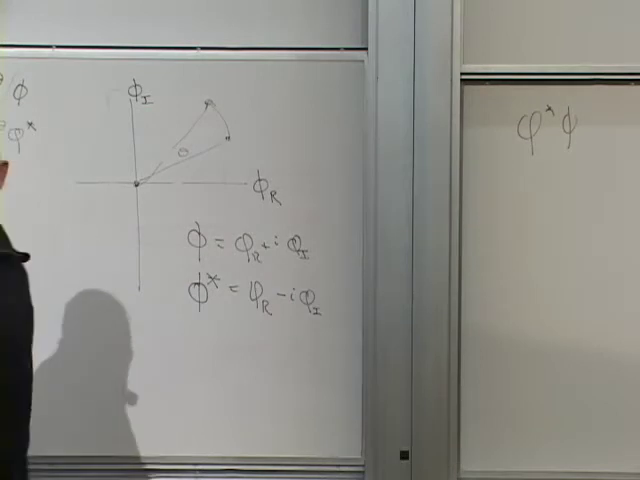
\includegraphics[width=0.80\textwidth]{lecture_07_figure_02.png}
\caption{Trường phức trên mặt phẳng nội tại \((\phi_R,\phi_I)\). Trên bảng ghi phép phân tích của \(\phi\) và \(\phi^*\) cùng bán kính bất biến \(\phi^*\phi\).}
\lectureframe{00:33:33}
\end{figure}

Sử dụng Lagrangian
\begin{equation}
  \mathcal L
  =\partial_\mu\phi^*\,\partial^\mu\phi
   -V(\phi^*\phi).
  \label{eq:l07-complex-lagrangian}
\end{equation}
Đối với trường phức, thừa số thông thường \(1/2\) không có mặt, vì riêng tích này đã chứa các hạng động học của cả hai thành phần thực.
Phép biến đổi
\begin{equation}
  \phi'(x)=e^{i\theta}\phi(x),
  \qquad
  \phi^{*\prime}(x)=e^{-i\theta}\phi^*(x)
  \label{eq:l07-global-u1}
\end{equation}
quay mọi giá trị của trường một góc như nhau. Ở đây \(\theta\) là hằng số theo không gian và thời gian. Dấu phẩy trên ký hiệu chỉ trường sau biến đổi; đó không phải là đạo hàm.

Vì \(\theta\) là hằng,
\begin{equation}
  \partial_\mu\phi'=e^{i\theta}\partial_\mu\phi,
  \qquad
  \partial_\mu\phi^{*\prime}
  =e^{-i\theta}\partial_\mu\phi^*.
\end{equation}
Các pha triệt tiêu nhau trong hạng động năng, và \(\phi^{*\prime}\phi'=\phi^*\phi\). Vì vậy, mọi thế chỉ phụ thuộc vào \(\phi^*\phi\) đều có cùng đối xứng ấy. Một hạng chỉ phụ thuộc riêng vào \(\phi_R\) sẽ chọn một hướng trong mặt phẳng nội tại và phá vỡ nó một cách tường minh.

\subsection{Một cực tiểu tại một điểm và một đường tròn các cực tiểu}

Có 2 loại thế đối xứng khác nhau về mặt định tính. Loại thứ nhất chỉ có cực tiểu duy nhất tại gốc, chẳng hạn
\begin{equation}
  V_{\rm unbroken}=m^2\phi^*\phi,
  \qquad m^2>0.
\end{equation}
Đồ thị của nó là một paraboloid đối xứng quay. Chân không \(\phi=0\) đứng yên dưới mọi phép quay, nên đối xứng là không bị phá vỡ.

Bây giờ hãy chọn
\begin{equation}
  V_{\rm broken}
  =-a\,\phi^*\phi+b(\phi^*\phi)^2,
  \qquad a,b>0.
  \label{eq:l07-mexican-hat}
\end{equation}
Hạng bậc hai âm đẩy trường ra xa gốc, còn hạng bậc bốn dương ngăn nó chạy ra vô cùng. Viết
\(r^2=\phi^*\phi\), việc cực tiểu hóa cho
\begin{equation}
  \frac{dV}{d(r^2)}=-a+2br^2=0,
  \qquad
  r^2=f^2=\frac{a}{2b}.
  \label{eq:l07-vacuum-radius}
\end{equation}
Vì thế, các cực tiểu tạo thành một đường tròn. Thế hoàn toàn đối xứng quay, nhưng một trạng thái cơ bản đồng đều buộc phải chọn một điểm trên đường tròn ấy.

\begin{figure}[htbp]
\centering
\includegraphics[width=0.72\textwidth]{lecture_07_figure_06.png}
\caption{Thế phá vỡ đối xứng được vẽ như một mặt tròn xoay. Gốc tọa độ là bất ổn và các cực tiểu suy biến tạo thành rãnh tròn.}
\lectureframe{00:37:25}
\end{figure}

Hãy hình dung trường như một mũi tên nhỏ trong mặt phẳng nội tại này tại mỗi điểm của không gian thông thường. Thế yêu cầu mọi mũi tên đều có độ dài \(f\). Năng lượng gradient yêu cầu các mũi tên lân cận chỉ gần như cùng một hướng. Vì vậy, trạng thái cơ bản có cùng một góc ở mọi nơi, nhưng không góc nào được định luật ưu tiên. Đó là sự phá vỡ tự phát của một đối xứng liên tục.

\section{Từ vách miền đến một xoắn trơn}

Hãy lặp lại thí nghiệm điều kiện biên. Ở biên trái, cố định trường tại một điểm chân không \(A\); ở biên phải, cố định nó tại một điểm chân không khác \(B\). Một bước nhảy cục bộ sẽ làm gradient lớn. Tuy nhiên, khác với trường hợp rời rạc, trường có thể vẫn nằm ở đáy của thế trong khi thay đổi liên tục quanh đường tròn.

Ở năng lượng thấp, viết trường thành \(\phi=f e^{i\alpha(x)}\). Trong 1 chiều không gian, năng lượng liên quan là
\begin{equation}
  E[\alpha]
  =f^2\int_0^L dx\,\left(\frac{d\alpha}{dx}\right)^2.
  \label{eq:l07-angle-functional}
\end{equation}
Với các góc ở hai đầu mút được cố định, phép biến phân cho
\begin{equation}
  \frac{d^2\alpha}{dx^2}=0,
  \qquad
  \alpha(x)=\alpha_A+
    \frac{\alpha_B-\alpha_A}{L}\,x.
  \label{eq:l07-linear-twist}
\end{equation}
Cấu hình được ưu tiên dàn đều độ xoắn trên toàn bộ mẫu. Năng lượng của nó tỉ lệ như
\begin{equation}
  E_{\rm twist}
  =f^2\frac{(\alpha_B-\alpha_A)^2}{L},
  \label{eq:l07-twist-energy}
\end{equation}
nên có thể làm cho nó rẻ tùy ý bằng cách tăng \(L\).

\begin{figure}[htbp]
\centering
\begin{adjustbox}{max width=\linewidth}
\begin{tikzpicture}[x=0.95cm,y=0.95cm]
  \begin{scope}
    \draw[->] (0,0) -- (6.2,0) node[right] {$x$};
    \draw[->] (0,0) -- (0,3.5) node[above] {$\alpha(x)$};
    \draw[very thick,blue!70!black] (0.45,0.65) -- (5.7,2.85);
    \fill (0.45,0.65) circle (1.8pt) node[left] {$\alpha_A$};
    \fill (5.7,2.85) circle (1.8pt) node[right] {$\alpha_B$};
    \node at (3.1,-0.65) {physical space};
  \end{scope}
  \begin{scope}[xshift=9.2cm,yshift=1.65cm]
    \draw[thick] (0,0) circle (1.8);
    \fill (1.55,-0.92) circle (1.8pt) node[below right] {$A$};
    \fill (-0.45,1.74) circle (1.8pt) node[above] {$B$};
    \draw[very thick,blue!70!black,-{Latex[length=2.5mm]}]
      (1.55,-0.92) arc[start angle=-31,end angle=104,radius=1.8];
    \node at (0,-2.35) {vacuum circle};
  \end{scope}
\end{tikzpicture}
\end{adjustbox}
\caption{Cùng một cấu hình năng lượng thấp trong 2 cách mô tả. Góc biến thiên tuyến tính theo không gian vật lý, trong khi trường đi theo cung ngắn của đường tròn chân không trong không gian nội tại.}
\end{figure}

\begin{classroomqa}
\audiencequestion{Có thể có hai cách đi quanh đường tròn. Trường đi theo lộ trình nào, và nó có thể bị mắc kẹt trên lộ trình dài hơn không?
\lecturetimestamp{00:41:54}}
\lecturerresponse{Với các điểm cuối tổng quát, lộ trình góc ngắn hơn có gradient nhỏ hơn và do đó năng lượng thấp hơn. Các điểm cuối đối diện nhau qua đường kính làm cho hai lộ trình đơn giản nhất suy biến. Một cấu hình được chuẩn bị bằng cách di chuyển chậm một điểm cuối có thể giữ lại một số quấn bổ sung và bị mắc kẹt sau một rào cản năng lượng, nhưng với một cặp điểm cuối thông thường đã cho thì lộ trình ngắn nhất không xoắn là trạng thái cơ bản.}
\end{classroomqa}

\begin{classroomqa}
\audiencequestion{Liệu một lộ trình có thể rời đáy rãnh và cắt ngang qua phần bên trong để trở nên ngắn hơn về tổng thể không?\lecturetimestamp{00:43:32}}
\lecturerresponse{Trong chế độ năng lượng thấp và mẫu dài, việc leo lên thế năng theo bán kính là không đáng. Giữ bán kính ở giá trị chân không của nó và cho góc biến thiên tuyến tính sẽ cực tiểu hóa năng lượng hiệu dụng, như phép tính giải tích biến phân ở trên cho thấy. Đối với một hệ hữu hạn với một thế năng cụ thể, ta có thể cực tiểu hóa đồng thời chuyển động theo bán kính và theo góc, nhưng kết luận Goldstone liên quan đến giới hạn bước sóng dài tùy ý, trong đó chuyển động trơn dọc theo rãnh thắng thế.}
\end{classroomqa}

\begin{classroomqa}
\audiencequestion{Điều gì thay đổi nếu rãnh tròn bị nghiêng đi sao cho một góc có năng lượng thấp hơn?\lecturetimestamp{00:44:33}}
\lecturerresponse{Khi đó đối xứng bị phá vỡ tường minh. Một điểm trở thành trạng thái cơ bản thực sự, chuyển động dọc theo đường tròn có lực hồi phục, và kích thích góc không còn chính xác là không khối lượng.}
\end{classroomqa}

\section{Khối lượng như cái giá của một dao động có xung lượng bằng không}

Sự xoắn trơn bộc lộ một trường mà năng lượng chỉ đến từ các gradient. Để hiểu vì sao điều đó có nghĩa là một hạt không khối lượng, hãy so sánh với hệ thức tán sắc tương đối tính
\begin{equation}
  \omega^2=\bm{k}^2+m^2.
  \label{eq:l07-dispersion}
\end{equation}
Một sóng \(e^{i(\bm{k}\cdot\bm{x}-\omega t)}\) mang xung lượng \(\bm{k}\).
Nếu \(m=0\), năng lượng của nó tiến về 0 khi bước sóng tiến tới vô hạn:
\(\omega=|\bm{k}|\to0\). Nếu \(m\ne0\), một mode đồng nhất theo không gian
\(\bm{k}=0\) vẫn dao động với tần số \(\omega=m\). Khối lượng là năng lượng bất khả quy ở xung lượng bằng không.

Sự phân biệt ấy cũng thấy được trong Lagrangian. Một hạng
\begin{equation}
  -\frac12m^2\varphi^2
\end{equation}
cung cấp một lực hồi phục ngay cả cho một dịch chuyển đồng nhất. Một trường chỉ có các hạng đạo hàm thì không có lực hồi phục như vậy: kéo dài bước sóng của nó ra, và năng lượng gradient của nó tiến tới 0.

\subsection{Biến cực tách hai mode}

Viết trường phức bị phá vỡ dưới dạng
\begin{equation}
  \phi(x)=\rho(x)e^{i\alpha(x)}.
  \label{eq:l07-polar}
\end{equation}
Cả \(\rho\) và \(\alpha\) đều là các trường. Lấy đạo hàm ta được
\begin{align}
  \partial_\mu\phi
  &=e^{i\alpha}
    \left(\partial_\mu\rho+i\rho\,\partial_\mu\alpha\right),\\
  \partial_\mu\phi^*
  &=e^{-i\alpha}
    \left(\partial_\mu\rho-i\rho\,\partial_\mu\alpha\right).
\end{align}
Các hạng chéo triệt tiêu, còn lại
\begin{equation}
  \partial_\mu\phi^*\,\partial^\mu\phi
  =(\partial_\mu\rho)(\partial^\mu\rho)
   +\rho^2(\partial_\mu\alpha)(\partial^\mu\alpha).
  \label{eq:l07-polar-kinetic}
\end{equation}
Vì \(\phi^*\phi=\rho^2\),
\begin{equation}
  \mathcal L
  =(\partial\rho)^2+\rho^2(\partial\alpha)^2-V(\rho^2).
  \label{eq:l07-polar-lagrangian}
\end{equation}
Thế năng chứa \(\rho\) nhưng không chứa \(\alpha\). Sự vắng mặt ấy là dạng hữu ích nhất của đối xứng.

\begin{figure}[htbp]
\centering
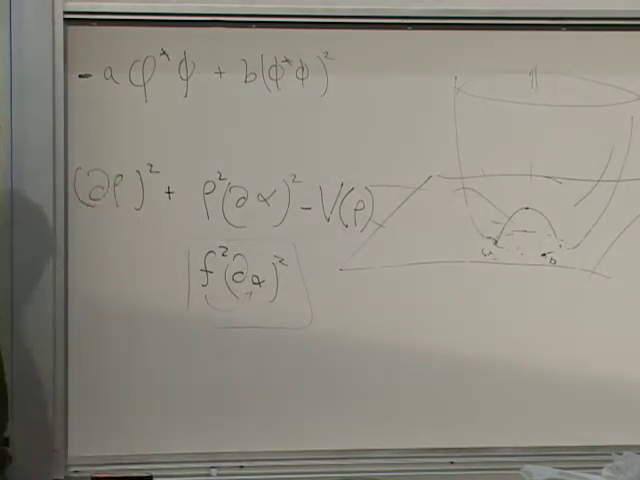
\includegraphics[width=0.88\textwidth]{lecture_07_figure_03.png}
\caption{Lagrangian của trường trong biến cực, hạng góc năng lượng thấp được đóng khung của nó, và thế năng phá vỡ đối xứng. Chuyển động theo bán kính leo lên thế năng; chuyển động theo góc đi dọc theo rãnh.}
\lectureframe{00:56:40}
\end{figure}

Đối với một kích thích năng lượng rất thấp, trường vẫn ở gần
\(\rho=f\). Khi đó
\begin{equation}
  \mathcal L_{\rm angular}
  \simeq f^2(\partial_\mu\alpha)(\partial^\mu\alpha).
\end{equation}
Định nghĩa trường góc được chuẩn hóa chính tắc, tùy theo quy ước dùng cho các thừa số \(1/2\), bằng
\begin{equation}
  \beta=\sqrt{2}\,f\alpha,
  \qquad
  \mathcal L_{\rm angular}
  =\frac12(\partial_\mu\beta)(\partial^\mu\beta).
  \label{eq:l07-goldstone-field}
\end{equation}
Không có hạng \(\beta^2\). Các lượng tử của trường góc này là không khối lượng. Chúng là các boson Goldstone.

Trường theo bán kính hành xử khác. Nếu dời \(\rho\) khỏi \(f\) đồng thời ở mọi nơi thì nó trở về, vượt quá, rồi dao động quanh rãnh. Nếu
\(\rho=f+h\), khai triển phương trình~\eqref{eq:l07-mexican-hat} cho
\begin{equation}
  V(f+h)=V(f)+\frac12m_h^2h^2+\cdots,
\end{equation}
nên \(h\) có khối lượng. Về mặt hình học, phương góc là phẳng còn phương bán kính là cong.

\begin{classroomqa}
\audiencequestion{Nếu trường bị lệch theo hướng xuyên tâm, liệu nó có đơn giản rơi trở lại xuống hay không, và sau đó điều gì xảy ra?\lecturetimestamp{00:57:10}}
\lecturerresponse{Nếu không có chuyển động góc, nó rơi về phía điểm cực tiểu, vượt quá điểm đó rồi dao động theo phương xuyên tâm. Một dao động đồng nhất có động lượng không gian bằng không nhưng tần số khác không; tần số đó là khối lượng của kích thích xuyên tâm. Ngược lại, một độ lệch góc đồng nhất đưa nó tới một chân không khác và không có lực phục hồi.}
\end{classroomqa}

Đây là nội dung của nguyên lý Goldstone trong ví dụ hiện tại: phá vỡ tự phát một đối xứng toàn cục liên tục sinh ra một mode không khối lượng cho mỗi phương phẳng độc lập của đa tạp chân không.
\editorialnote{Mệnh đề này giả sử các điều kiện thông thường của lý thuyết trường tương đối tính. Trong các hệ nhiều hạt phi tương đối tính, việc đếm số và quan hệ tán sắc của các mode Nambu--Goldstone có thể tinh tế hơn, nhưng kết luận ở giới hạn bước sóng dài của bài giảng vẫn là kết luận đúng cho mô hình \(U(1)\) tương đối tính này.}

\section{Sóng spin, dây và âm thanh}

Định lý thì trừu tượng, nhưng cơ chế của nó lại quen thuộc. Trong một sắt từ đẳng hướng, mọi spin có thể cùng quay mà không làm thay đổi năng lượng. Cho hướng đó biến thiên rất chậm trên toàn mẫu, ta thu được một sóng spin. Năng lượng phải trả cho nó triệt tiêu cùng với số sóng của nó, nên nó là mode Goldstone của đối xứng quay spin bị phá vỡ.

Một sợi dây đàn hồi dài cho ta một hình dung khác. Bỏ qua trọng lực và gắn hai đầu sao cho toàn bộ sợi dây có thể được tịnh tiến theo phương thẳng đứng. Một phép tịnh tiến thẳng đứng đồng nhất không tốn năng lượng. Nếu cho phép tịnh tiến đó biến thiên chậm dọc theo dây thì nó trở thành một sóng ngang bước sóng dài. Phép tác động đối xứng đồng nhất đã được nâng thành một biến dạng nhẹ phụ thuộc vị trí.

\begin{figure}[htbp]
\centering
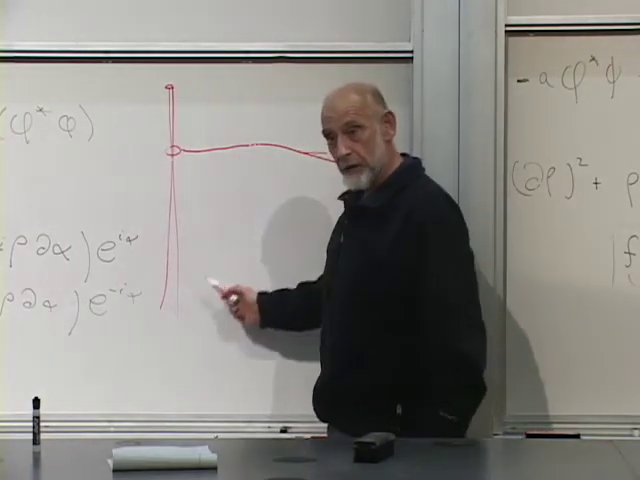
\includegraphics[width=0.68\textwidth]{lecture_07_figure_04.png}
\caption{Biên dạng sợi dây biến thiên chậm được vẽ trong phép tương tự mode Goldstone. Điểm vật lý là độ dốc nhỏ của một biến dạng bước sóng dài, chứ không phải vị trí theo phương thẳng đứng của đường cong.}
\lectureframe{01:04:19}
\end{figure}

\begin{classroomqa}
\audiencequestion{Sợi dây có thể mang năng lượng dao động trong khi có xung lượng bằng 0 không?\lecturetimestamp{01:04:41}}
\lecturerresponse{Cần phân biệt xung lượng cơ học theo phương thẳng đứng với xung lượng sóng dọc theo dây. Một sóng dừng có thể có tổng xung lượng bằng 0 vì nó là chồng chập của các mode có \(+k\) và \(-k\), trong khi vẫn mang năng lượng. Trong phép tương tự lý thuyết trường, xung lượng ám chỉ số sóng dọc theo trục; độ dời theo phương thẳng đứng đóng vai trò tọa độ nội tại của trường.}
\end{classroomqa}

Một lò xo slinky cho phiên bản dọc. Tịnh tiến toàn bộ lò xo slinky vô hạn lý tưởng hóa dọc theo trục của nó thì không có gì thay đổi. Tịnh tiến các phần lân cận những lượng hơi khác nhau thì kết quả là một sóng nén nhẹ. Trong chất rắn hoặc chất lưu, âm thanh bước sóng dài cũng tương tự như vậy, nảy sinh từ các độ dời tập thể và các biến thiên mật độ. Sóng spin, sóng ngang trên dây, và âm thanh không phải là cùng một kích thích vi mô, nhưng chúng chia sẻ khuôn mẫu quyết định: một phép tác động liên tục đồng nhất không tốn năng lượng, và phiên bản biến thiên chậm của nó trở thành một mode mềm.
\editorialnote{Trong tinh thể, các phonon âm học theo quy ước được mô tả là các mode Nambu--Goldstone của các phép tịnh tiến liên tục bị phá vỡ tự phát. Dây và lò xo slinky là những phép tương tự cơ học được dùng trong bài giảng để phơi bày cùng một cấu trúc năng lượng chỉ gồm đạo hàm.}

Thuật ngữ đủ quan trọng để có một câu đùa ngắn trên lớp: đây là các boson \emph{Goldstone}, được đặt theo tên Jeffrey Goldstone, chứ không phải boson chuẩn. Bài giảng lưu ý rằng Goldstone là bạn của Susskind, rồi chuyển sang chủ đề thực sự khác là bất biến chuẩn.

\section{Từ đối xứng pha toàn cục đến đối xứng chuẩn}

Đối xứng pha \(U(1)\) đã xuất hiện trong môn học này như là đối xứng gắn với sự bảo toàn điện tích. Các trường hạt mang điện là các trường phức, và việc nhân một trường như vậy với một pha chung không làm thay đổi lý thuyết toàn cục. Có thể dùng từ điện để trực giác hóa, dù điện tích ấy cũng có thể biểu diễn một số lượng tử \(U(1)\) khác. Photon thật sự là không khối lượng; đích đến cuối cùng là một trường kiểu photon như \(Z\) có khối lượng.

Câu hỏi mới là liệu
\begin{equation}
  \phi'(x)=e^{i\theta(x)}\phi(x)
  \label{eq:l07-local-u1}
\end{equation}
có thể là một đối xứng khi \(\theta\) biến thiên tùy ý trong không-thời gian hay không. Hàm \(\theta(x)\) là một tham số biến đổi, không phải một trường động lực bổ sung. Ta kiểm tra đề xuất này bằng cách lấy đạo hàm:
\begin{equation}
  \partial_\mu\phi'
  =e^{i\theta}
   \left[\partial_\mu\phi+i(\partial_\mu\theta)\phi\right].
  \label{eq:l07-local-derivative}
\end{equation}
Hạng phụ thêm đó vắng mặt khi \(\theta\) là hằng. Đối với trường liên hợp,
\begin{equation}
  \partial_\mu\phi^{*\prime}
  =e^{-i\theta}
   \left[\partial_\mu\phi^*-i(\partial_\mu\theta)\phi^*\right].
\end{equation}
Tích của chúng là
\begin{align}
  \partial_\mu\phi^{*\prime}\partial^\mu\phi'
  ={}&
  \partial_\mu\phi^*\partial^\mu\phi
  i\left(
      \phi\,\partial_\mu\phi^*
      -\phi^*\partial_\mu\phi
    \right)\partial^\mu\theta
  \nonumber\\
  &+\phi^*\phi\,
    \partial_\mu\theta\,\partial^\mu\theta.
  \label{eq:l07-local-failure}
\end{align}
Thế năng vẫn bất biến vì \(\phi^*\phi\) bất biến, nhưng hạng động năng thông thường thì không còn như vậy. Một đối xứng toàn cục không tự động trở thành một đối xứng cục bộ.

\begin{classroomqa}
\audiencequestion{Trong hình chiếc mũ Mexico, sự thất bại này có nghĩa là có những gợn nhô quanh rãnh tròn không?\lecturetimestamp{01:19:37}}
\lecturerresponse{Không. Thế năng vẫn có thể hoàn toàn phẳng theo phương góc. Cái giá phụ thêm đến từ các gradient khi pha khác nhau từ điểm không-thời gian này sang điểm không-thời gian khác. Đó không phải là sự nhấp nhô của rãnh; đó là hạng đạo hàm thông thường đang phát hiện sự biến thiên theo không gian.}
\end{classroomqa}

\subsection{Trường vectơ bù}

Các tương tác của photon, \(W\), \(Z\) và gluon trong tự nhiên được tổ chức bởi các đối xứng chuẩn cục bộ, chứ không chỉ bởi các phép biến đổi cứng. Để biến phép tác động pha cục bộ thành một đối xứng, hãy mở rộng lý thuyết bằng một trường bốn-vectơ \(A_\mu\). Trong điện từ học, \(A_0\) là thế vô hướng còn ba thành phần không gian tạo thành thế vectơ. Các đạo hàm của chúng tạo nên điện trường và từ trường.

Hãy chọn quy ước tự nhất quán
\begin{equation}
  \phi'=e^{i\theta}\phi,
  \qquad
  A'_\mu=A_\mu-\partial_\mu\theta,
  \qquad
  D_\mu=\partial_\mu+iA_\mu.
  \label{eq:l07-gauge-convention}
\end{equation}
Trên bảng, một dấu bị đổi trong lúc kiểm tra sự triệt tiêu; phương trình \eqref{eq:l07-gauge-convention} cố định đồng thời cả ba dấu. Hằng số ghép chuẩn và điện tích đã tạm thời được hấp thụ vào \(A_\mu\).
\editorialnote{Khi viết tường minh điện tích \(q\) và hằng số ghép \(g\), ta có thể viết \(D_\mu=\partial_\mu+igqA_\mu\) và
\(A'_\mu=A_\mu-(gq)^{-1}\partial_\mu\theta\). Bài giảng lược bỏ các hằng số này để sự triệt tiêu vẫn hiển lộ.}

Đối với trường liên hợp,
\begin{equation}
  D_\mu\phi^*=\partial_\mu\phi^*-iA_\mu\phi^*.
\end{equation}
Bây giờ
\begin{align}
  D'_\mu\phi'
  &=
  \left(\partial_\mu+iA'_\mu\right)e^{i\theta}\phi
  \nonumber\\
  &=
  e^{i\theta}
  \left[
    \partial_\mu\phi+i(\partial_\mu\theta)\phi
    +i(A_\mu-\partial_\mu\theta)\phi
  \right]
  \nonumber\\
  &=e^{i\theta}D_\mu\phi.
  \label{eq:l07-covariant-transform}
\end{align}
Đạo hàm không mong muốn của \(\theta\) được triệt tiêu bởi phép biến đổi của \(A_\mu\). Tương tự,
\begin{equation}
  D'_\mu\phi^{*\prime}=e^{-i\theta}D_\mu\phi^*.
\end{equation}
Tích của chúng là bất biến. Tính từ \emph{hiệp biến} có nghĩa là đạo hàm biến đổi theo cùng một cách đơn giản như chính trường đó.

\section{Động lực học của trường chuẩn}

Nếu chỉ đưa \(A_\mu\) vào để sửa một đạo hàm thì nó sẽ không có động lực học riêng. Cường độ trường bất biến chuẩn là
\begin{equation}
  F_{\mu\nu}
  =\partial_\mu A_\nu-\partial_\nu A_\mu.
  \label{eq:l07-field-strength}
\end{equation}
Nó là phản đối xứng, nên \(F_{\mu\mu}=0\). Các thành phần thời gian--không gian của nó chứa điện trường, còn các thành phần không gian--không gian chứa từ trường. Trong ngôn ngữ ba-vectơ quen thuộc, mật độ năng lượng điện từ tỉ lệ với \(\bm E^2+\bm B^2\), còn Lagrangian Lorentz tỉ lệ với \(\bm E^2-\bm B^2\), với các dấu phụ thuộc vào quy ước metric.

\begin{classroomqa}
\audiencequestion{Năng lượng và Lagrangian của trường điện từ là gì?\lecturetimestamp{01:33:20}}
\lecturerresponse{Năng lượng được xây dựng từ \(E^2+B^2\); Lagrangian dùng \(E^2-B^2\). Trong dạng hiệp biến, đại lượng sau được viết như một bội số theo quy ước của \(F_{\mu\nu}F^{\mu\nu}\). Tensor phản đối xứng đó là xoáy bốn chiều của thế vectơ.}
\end{classroomqa}

Bản thân cường độ trường cũng bất biến chuẩn:
\begin{align}
  F'_{\mu\nu}
  &=
  \partial_\mu(A_\nu-\partial_\nu\theta)
  -\partial_\nu(A_\mu-\partial_\mu\theta)
  \nonumber\\
  &=
  F_{\mu\nu}
  -\partial_\mu\partial_\nu\theta
  +\partial_\nu\partial_\mu\theta
  =F_{\mu\nu}.
  \label{eq:l07-field-strength-invariant}
\end{align}
Đẳng thức cuối cùng suy ra vì các đạo hàm riêng hỗn hợp thông thường giao hoán. Do đó, một Lagrangian bất biến chuẩn tiêu chuẩn là
\begin{equation}
  \boxed{
  \mathcal L
  =(D_\mu\phi)^*D^\mu\phi
  -V(\phi^*\phi)
  -\frac14F_{\mu\nu}F^{\mu\nu}}
  \label{eq:l07-scalar-qed}
\end{equation}
tùy theo quy ước về dấu và chuẩn hóa được chọn cho metric.

\begin{figure}[htbp]
\centering
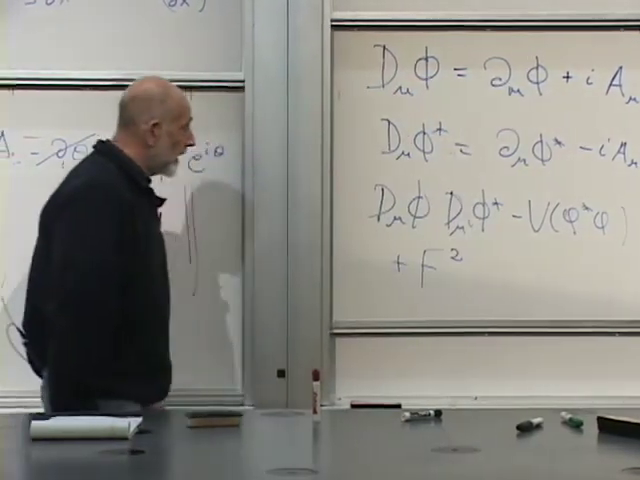
\includegraphics[width=0.84\textwidth]{lecture_07_figure_05.png}
\caption{Các đạo hàm hiệp biến và Lagrangian bất biến chuẩn được ghép lại trên bảng. Các thừa số số học được lược bỏ ở đó để cấu trúc biến đổi vẫn hiển lộ.}
\lectureframe{01:38:45}
\end{figure}

Cấu trúc này nâng một đối xứng toàn cục \(U(1)\) thành một đối xứng cục bộ, nhưng nó làm như vậy với cái giá---hay, về mặt vật lý, với món quà---là một trường vectơ mới. Trong ví dụ Abel, trường ấy chính là thế điện từ.

\begin{classroomqa}
\audiencequestion{Lagrangian ban đầu của ta dùng các đạo hàm thường. Vì sao chúng ta có quyền thay chúng bằng các đạo hàm hiệp biến và gọi kết quả là lý thuyết thực sự?\lecturetimestamp{01:42:55}}
\lecturerresponse{Chúng ta đang xây dựng một lý thuyết khác, được mở rộng: vật chất mang điện cộng với một trường chuẩn. Bất biến chuẩn cục bộ quyết định sự ghép của chúng. Lý thuyết lượng tử thu được là một cấu trúc toán học nhất quán và phù hợp với cách tự nhiên tổ chức photon và các trường chuẩn yếu. Chỉ riêng việc ghép một trường vectơ tương đối tính một cách không nhất quán có thể đưa vào các phân cực phi vật lý và sự vi phạm xác suất, vì vậy nguyên lý chuẩn không phải là một phép viết lại mang tính hình thức của lý thuyết vô hướng tự do cũ.}
\end{classroomqa}

\begin{classroomqa}
\audiencequestion{Vậy việc thêm trường mới chính là cơ sở biện minh cốt yếu cho sự sửa đổi này sao?\lecturetimestamp{01:44:57}}
\lecturerresponse{Đúng. Không có \(A_\mu\), đạo hàm của một trường sau phép quay cục bộ sẽ chứa một \(\partial_\mu\theta\) không bị triệt tiêu. Với \(A_\mu\) và quy luật biến đổi của nó, sự triệt tiêu diễn ra. Trong ngôn ngữ hình học, \(A_\mu\) là một liên hệ trên một bó sợi; phần toán học sâu hơn đó là có thật và hữu ích, nhưng phần đại số ở trên đã chứa điều cần thiết ở đây.}
\end{classroomqa}

\section{Vì sao khối lượng trần của boson chuẩn lại bị cấm}

Đối với một trường boson thông thường, khối lượng được biểu diễn bằng một số hạng bậc hai.
Ta rất dễ muốn thêm
\begin{equation}
  \Delta\mathcal L_{\rm Proca}
  =\frac12m^2A_\mu A^\mu.
  \label{eq:l07-proca}
\end{equation}
Nhưng dưới \(A_\mu\mapsto A_\mu-\partial_\mu\theta\),
\begin{equation}
  A'_\mu A^{\mu\prime}
  =
  A_\mu A^\mu
  -2A^\mu\partial_\mu\theta
  +\partial_\mu\theta\,\partial^\mu\theta,
\end{equation}
nên phương trình~\eqref{eq:l07-proca} không bất biến chuẩn. Ta không thể đưa một khối lượng vào lý thuyết chuẩn này bằng tay mà vẫn giữ đối xứng cục bộ của nó.

\begin{figure}[htbp]
\centering
\includegraphics[width=0.72\textwidth]{lecture_07_figure_07.png}
\caption{Số hạng khối lượng vectơ trần được đề xuất \(\tfrac12m^2A_\mu A^\mu\). Sự thất bại của nó dưới \(A_\mu\mapsto A_\mu-\partial_\mu\theta\) là chướng ngại dẫn tới cơ chế Higgs.}
\lectureframe{01:39:48}
\end{figure}

Đây là thế bế tắc bề ngoài. Bất biến chuẩn giải thích photon không khối lượng và bảo vệ lý thuyết khỏi các bậc tự do phi vật lý, nhưng \(W\) và \(Z\) lại có khối lượng. Lối thoát không thể là một khối lượng vectơ tường minh. Nó phải phát sinh từ các trường đã có mặt trong một Lagrangian bất biến chuẩn.

\begin{classroomqa}
\audiencequestion{Việc đưa bất biến chuẩn vào tự nó có sinh ra boson Goldstone không?\lecturetimestamp{01:45:51}}
\lecturerresponse{Không. Boson Goldstone xuất hiện khi một đối xứng \emph{toàn cục} liên tục bị phá vỡ tự phát, trước khi thế vectơ được đưa vào. Khi đối xứng trở thành cục bộ, một pha biến thiên có thể được bù bởi \(A_\mu\). Trong lý thuyết chuẩn bị phá vỡ, mode góc không còn là một hạt không khối lượng độc lập nữa; nó cung cấp phân cực bổ sung của trường vectơ nay đã có khối lượng. Bài giảng tiếp theo sẽ suy ra phát biểu đó chứ không chỉ đơn thuần tuyên bố nó.}
\end{classroomqa}

\begin{classroomqa}
\audiencequestion{Có điều nào trong số này giải thích được vì sao các con sông uốn khúc không?\lecturetimestamp{01:47:03}}
\lecturerresponse{Không biết có mối liên hệ trực tiếp nào ở đây. Các xoáy trong chất lỏng và thậm chí cả hình dạng của sinh vật chắc chắn có thể được mô tả bằng các phương pháp đối xứng, và ta không bao giờ nên ngạc nhiên khi bắt gặp các ý tưởng của lý thuyết trường ở những nơi bất ngờ, nhưng bài giảng này không hề nêu ra một lý thuyết chuẩn về sự uốn khúc của sông.}
\end{classroomqa}

\section{Điểm dừng của bài giảng}

Giờ đây ta đã có hai thành phần đã hứa ở phần đầu. Một đối xứng toàn cục liên tục với một đường tròn các chân không có một hướng góc phẳng, và sự biến thiên chậm của nó là một trường Goldstone không khối lượng. Một đối xứng cục bộ đòi hỏi một liên hệ chuẩn và các đạo hàm hiệp biến, đồng thời cấm khối lượng vectơ trực tiếp trong phương trình~\eqref{eq:l07-proca}.

Bước tiếp theo là dùng thế năng bị phá vỡ của phương trình~\eqref{eq:l07-mexican-hat} trong lý thuyết bất biến chuẩn của phương trình~\eqref{eq:l07-scalar-qed}. Khi đó hai điều xảy ra đồng thời: hạt Goldstone riêng rẽ biến mất khỏi phổ vật lý, và trường vectơ thu được khối lượng. Theo ngôn ngữ sư phạm thông dụng, đối xứng chuẩn bị phá vỡ tự phát; chính xác hơn, sự dư thừa chuẩn vẫn còn nguyên trong khi lý thuyết đi vào một pha Higgs với một kích thích vectơ có khối lượng.
\editorialnote{Một đối xứng chuẩn cục bộ là sự dư thừa trong mô tả chứ không phải một đối xứng vật lý thông thường tác dụng giữa các trạng thái quan sát được phân biệt. Bài giảng dùng lối nói tắt tiêu chuẩn về sự phá vỡ tự phát của đối xứng chuẩn. Phát biểu vật lý bất biến chuẩn là sự sắp xếp lại các bậc tự do trong pha Higgs.}

Đó là hiện tượng Higgs. Chúng ta vẫn chưa thực hiện nó. Bài giảng này đã làm phần việc khó hơn nhưng cần thiết là làm cho bài toán đủ chính xác để khi lời giải xuất hiện, nó sẽ là điều không thể tránh khỏi.
\chapter{Cơ chế Higgs: Cách một boson chuẩn thu được khối lượng}

Bây giờ ta kết hợp hai ý tưởng đã được phát triển trong bài giảng trước. Một trường vô hướng phức với đối xứng toàn cục \(U(1)\) bị phá vỡ chứa một dao động hướng tâm có khối lượng và một dao động góc không khối lượng. Một lý thuyết \(U(1)\) bất biến cục bộ chứa một trường chuẩn không khối lượng. Khi trường vô hướng mang điện tích và độ lớn cân bằng của nó khác không, không thể đơn giản cộng gộp các phát biểu này với nhau. Mode góc và trường chuẩn kết hợp với nhau: trường chuẩn trở nên có khối lượng, boson Goldstone biểu kiến không còn là một hạt độc lập nữa, còn mode Higgs hướng tâm vẫn còn lại.

Photon sẽ là boson chuẩn mô hình của ta, nhưng không phải kết luận vật lý của ta. \(U(1)\) điện từ không bị phá vỡ trong chân không, nên photon thực là không khối lượng. Cùng cơ chế ấy tác dụng lên \(W^\pm\) và \(Z\) trong lý thuyết điện yếu, nơi nhóm chuẩn và đa bội vô hướng phức tạp hơn. Mô hình abel làm lộ rõ cơ chế mà không che khuất nó dưới lớp lý thuyết nhóm.

\begin{classroomqa}
\audiencequestion{Liệu phần thảo luận trước có hàm ý rằng cơ chế Higgs cấp khối lượng cho photon thực không?\lecturetimestamp{00:00:23}}
\lecturerresponse{Không. Ta đang hỏi điều gì sẽ xảy ra \emph{nếu} \(U(1)\) gắn với photon ở trong một pha bị phá vỡ. Photon giả định đó sẽ trở nên có khối lượng. Chân không điện từ thực không ở trong pha ấy; thay vào đó, ứng dụng vào vật lý hạt là khối lượng của \(W\) và \(Z\).}
\end{classroomqa}

Đối xứng gắn với bảo toàn điện tích là phép quay pha
\begin{equation}
  \phi(x)\longmapsto e^{i\theta}\phi(x),
\end{equation}
một phép quay nội được gọi là \(U(1)\). Chất siêu dẫn cung cấp một tương tự thực của pha bị phá vỡ. Bên trong nó, trường điện từ có độ sâu xuyên thấu hữu hạn và xét trên những phương diện quan trọng thì ứng xử như một trường có khối lượng. Bên ngoài nó, photon thông thường không khối lượng lại xuất hiện.

\section{Khối lượng có nghĩa gì đối với một trường}

\subsection{Tán sắc và khe hở ở động lượng bằng không}

Trước khi đưa vào trường Higgs, ta nên xác định chính xác điều ta muốn nói bởi khối lượng. Đối với một sóng,
\begin{equation}
  E=\hbar\omega,
  \qquad
  p=\hbar k,
  \label{eq:l08-quantum-wave}
\end{equation}
vì vậy đồ thị \((E,p)\) và đồ thị \((\omega,k)\) chứa cùng một thông tin, sai khác chỉ ở các hệ số \(\hbar\). Trong không gian trống, một kích thích tương đối tính không khối lượng tuân theo
\begin{equation}
  E=c|p|,
  \qquad
  \omega=c|k|.
  \label{eq:l08-massless-dispersion}
\end{equation}
Hai dấu của \(k\) phân biệt hai hướng lan truyền đối ngược. Điểm cốt yếu là \(\omega\) tiến về 0 cùng với \(k\).

Một hạt tương đối tính có khối lượng tuân theo
\begin{equation}
  E^2=c^2p^2+m^2c^4.
  \label{eq:l08-massive-dispersion}
\end{equation}
Trong các đơn vị \(c=\hbar=1\),
\begin{equation}
  \omega^2=k^2+m^2.
\end{equation}
Tại \(k=0\), năng lượng là \(E=mc^2\), hay đơn giản là \(m\) trong đơn vị tự nhiên. Vì thế, khối lượng là khe hở năng lượng khác không của mode có động lượng bằng không.

\begin{figure}[htbp]
\centering
\begin{adjustbox}{max width=\linewidth}
\begin{tikzpicture}[x=1.05cm,y=1.05cm]
  \begin{scope}
    \draw[->] (-0.2,0) -- (4.2,0) node[right] {\(k\)};
    \draw[->] (0,-0.2) -- (0,3.1) node[above] {\(\omega\)};
    \draw[very thick,blue!65!black] (0,0) -- (3.8,2.75);
    \draw[very thick,orange!70!black] (0,0) -- (3.8,1.75);
    \node[blue!65!black,rotate=36] at (2.65,2.15)
      {\(\omega=c_{\rm vac}k\)};
    \node[orange!70!black,rotate=24] at (2.65,1.05)
      {ordinary medium};
    \node[below] at (2,-0.45) {gapless};
  \end{scope}
  \begin{scope}[xshift=6.2cm]
    \draw[->] (-0.2,0) -- (4.2,0) node[right] {\(k\)};
    \draw[->] (0,-0.2) -- (0,3.1) node[above] {\(\omega\)};
    \draw[very thick,domain=0:3.8,samples=120,smooth,teal!70!black]
      plot (\x,{sqrt(0.9+0.45*\x*\x)});
    \draw[dashed] (0,0.95) -- (1.0,0.95);
    \node[left] at (0,0.95) {\(m\)};
    \node[teal!70!black] at (2.55,2.15)
      {\(\omega^2=k^2+m^2\)};
    \node[below] at (2,-0.45) {gapped};
  \end{scope}
\end{tikzpicture}
\end{adjustbox}
\caption{Thay đổi tốc độ lan truyền sẽ làm thay đổi độ dốc của một quan hệ tán sắc không có khe hở. Gán khối lượng cho kích thích sẽ mở ra một khe hở khác không tại \(k=0\).}
\label{fig:l08-dispersion}
\end{figure}

Một vật liệu trong suốt thông thường có thể làm giảm vận tốc pha của sóng mà không tạo ra khe hở khối lượng tương đối tính này. Tại một biên, tần số tới được giữ cố định, còn số sóng thì tự điều chỉnh theo quan hệ tán sắc của môi trường. Thay đổi độ dốc không đồng nghĩa với việc nâng tung độ gốc lên.
\editorialnote{Một vật liệu có thể có vài nhánh điện từ, và plasma hoặc môi trường cộng hưởng có thể có một khe hở tần số plasma khác không. Phép so sánh trong bài giảng cụ thể là giữa một nhánh khúc xạ thông thường và đáp ứng siêu dẫn. Tổng quát hơn, tính không khe hở có nghĩa là \(\omega(k)\to0\) khi \(k\to0\); không phải trong mọi môi trường phi tương đối tính đều cần tính tuyến tính chính xác.}

\begin{classroomqa}
\audiencequestion{Có phải photon thu được khối lượng mỗi khi nó truyền qua vật chất, chẳng hạn qua một lăng kính không?\lecturetimestamp{00:03:02}}
\lecturerresponse{Không. Hiện tượng khúc xạ có thể làm thay đổi quan hệ giữa tần số và số sóng, và do đó thay đổi tốc độ lan truyền, trong khi nhánh đó vẫn đi qua \(\omega=0\) tại \(k=0\). Trái lại, một pha siêu dẫn làm cho đáp ứng điện từ có một nghịch đảo độ sâu xuyên thấu hữu hạn, là tương tự của khối lượng.}
\end{classroomqa}

\begin{classroomqa}
\audiencequestion{Đối với ánh sáng có tần số cố định đi vào thủy tinh, có phải số sóng là đại lượng thay đổi không?\lecturetimestamp{00:09:20}}
\lecturerresponse{Đúng. Tính bất biến theo tịnh tiến thời gian tại một mặt phân cách đứng yên giữ cho tần số không đổi. Vì đường cong tán sắc có độ dốc khác trong thủy tinh, cùng một \(\omega\) tương ứng với một \(k\) khác, và do đó với một bước sóng khác.}
\end{classroomqa}

Độ dốc
\begin{equation}
  v_g=\frac{d\omega}{dk}
\end{equation}
là vận tốc nhóm của một gói sóng. Nếu độ dốc ấy biến thiên theo \(k\), các thành phần Fourier khác nhau sẽ chuyển động với những tốc độ khác nhau và gói sóng sẽ tán ra. Đó là lý do quan hệ \(\omega(k)\) được gọi là \emph{quan hệ tán sắc}.

\begin{classroomqa}
\audiencequestion{Đường cong ấy được gọi là gì, và độ dốc của nó biểu diễn điều gì?\lecturetimestamp{00:11:02}}
\lecturerresponse{Đường cong đó là quan hệ tán sắc. Đạo hàm của nó \(d\omega/dk\) là vận tốc nhóm. Một độ dốc không đổi cho cùng một vận tốc đối với mọi bước sóng; một độ dốc biến thiên làm gói sóng loe ra. Với mục đích hiện tại, điểm phân biệt có tính quyết định là liệu đường cong có chạm tới gốc tọa độ hay có một khe hở.}
\end{classroomqa}

\subsection{Một dao động đồng nhất là một hạt đứng yên}

Mode \(k=0\) có bước sóng vô hạn: trường bị dịch đi cùng một lượng ở mọi nơi. Hãy thả tự do một dịch chuyển đồng nhất. Nếu trường dao động với tần số khác không, lượng tử tương ứng có năng lượng nghỉ khác không và là có khối lượng. Nếu không có lực phục hồi theo hướng đó, tần số triệt tiêu và mode là không khối lượng.

Phát biểu này là cổ điển. Nó không đòi hỏi các hạt tách biệt trong không gian phải ở trong một chồng chập lượng tử. Một cấu hình trường cổ điển đồng nhất đơn giản chỉ là một giá trị trường được lặp lại khắp không gian.

\begin{classroomqa}
\audiencequestion{Nếu toàn bộ một trường cùng bị dịch chuyển, điều đó có giống với sự vướng víu lượng tử không?\lecturetimestamp{00:10:04}}
\lecturerresponse{Không. Một trường cổ điển đồng nhất là một cấu hình cổ điển duy nhất. Sự vướng víu tương quan các khả năng lượng tử phân biệt, chẳng hạn các cấu hình spin lên--xuống và xuống--lên. Việc chuẩn bị cùng một giá trị trường tại nhiều điểm tự nó không phải là vướng víu, cũng không hàm ý một đáp ứng nhân quả tức thời.}
\end{classroomqa}

Đối với một trường thực được chuẩn hoá chuẩn tắc,
\begin{equation}
  \mathcal L
  =\frac12\partial_\mu\varphi\,\partial^\mu\varphi-V(\varphi),
\end{equation}
khai triển quanh một trạng thái cân bằng \(\varphi_0\):
\begin{equation}
  V(\varphi_0+\eta)
  =V(\varphi_0)
   +\frac12V''(\varphi_0)\eta^2+\cdots.
\end{equation}
Số hạng tuyến tính triệt tiêu tại điểm cực tiểu, và phương trình trường cho
\begin{equation}
  \omega^2=\bm{k}^2+m^2,
  \qquad
  m^2=V''(\varphi_0).
  \label{eq:l08-curvature-mass}
\end{equation}
Vì thế, khối lượng là độ cong của thế năng theo hướng chuyển động. Một hướng phẳng có độ cong bằng không và cho ra một mode không khối lượng.

\section{Trường vô hướng phức bị phá vỡ}

\subsection{Chuyển động theo phương bán kính và chuyển động góc}

Hãy viết một trường vô hướng phức trong tọa độ Descartes và tọa độ cực:
\begin{equation}
  \phi=\phi_R+i\phi_I=\rho e^{i\alpha},
  \qquad
  \phi^*=\phi_R-i\phi_I=\rho e^{-i\alpha}.
  \label{eq:l08-polar-field}
\end{equation}
Mặt phẳng phức là một không gian trường \emph{nội}. Tại mỗi điểm không-thời gian vật lý \(x\), cặp
\((\phi_R(x),\phi_I(x))\)
chỉ định một điểm trong mặt phẳng nội đó. Không trục nội nào là một phương trong phòng thí nghiệm.

\begin{figure}[htbp]
\centering
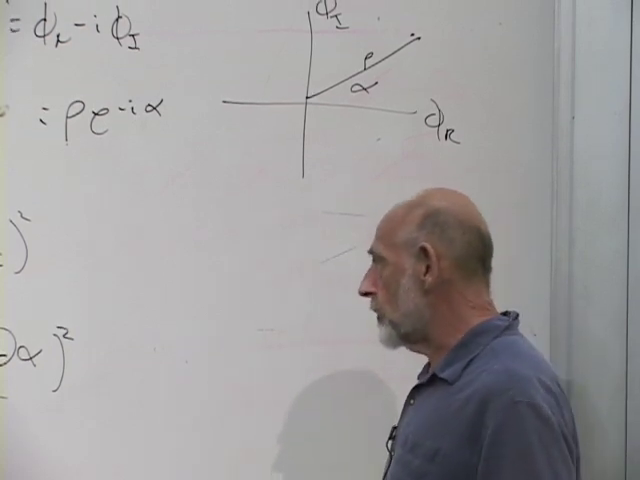
\includegraphics[width=0.72\textwidth]{lecture_08_figure_02.png}
\caption{Trường vô hướng phức được biểu diễn trong mặt phẳng \((\phi_R,\phi_I)\) nội của nó. Bán kính là \(\rho\), còn \(\alpha\) là pha nội.}
\lectureframe{00:24:41}
\label{fig:l08-internal-plane}
\end{figure}

Số hạng động học của trường vô hướng trở thành
\begin{align}
  \partial_\mu\phi^*\,\partial^\mu\phi
  &=
  \partial_\mu\phi_R\,\partial^\mu\phi_R
  +\partial_\mu\phi_I\,\partial^\mu\phi_I
  \notag\\
  &=
  \partial_\mu\rho\,\partial^\mu\rho
  +\rho^2\partial_\mu\alpha\,\partial^\mu\alpha.
  \label{eq:l08-polar-kinetic}
\end{align}
Một thế năng bất biến \(U(1)\) toàn cục phụ thuộc vào
\(\phi^*\phi=\rho^2\), chứ không phụ thuộc vào \(\alpha\). Chẳng hạn,
\begin{equation}
  V(\phi)
  =\lambda\left(\phi^*\phi-\frac{f^2}{2}\right)^2,
  \qquad \lambda>0.
  \label{eq:l08-mexican-hat}
\end{equation}
Các cực tiểu của nó tạo thành một vòng tròn. Quy luật này bất biến dưới một phép quay pha chung, nhưng việc chọn một pha cân bằng sẽ chọn ra một điểm trên vòng tròn.

\begin{figure}[htbp]
\centering
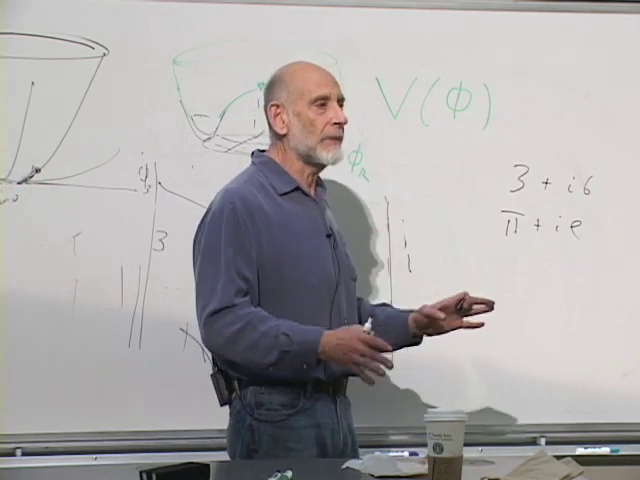
\includegraphics[width=0.78\textwidth]{lecture_08_figure_03.png}
\caption{Các phác họa thế năng hướng tâm trên bảng. Thế năng đối xứng dưới các phép quay của giá trị trường nội, mặc dù bản thân trường không nhất thiết phải nằm tại gốc tọa độ.}
\lectureframe{00:34:22}
\label{fig:l08-radial-potential-board}
\end{figure}

\begin{figure}[htbp]
\centering
\begin{tikzpicture}[x=0.94cm,y=0.94cm]
  \draw[->] (-4.2,0) -- (4.4,0) node[right] {\(\phi_R\)};
  \draw[->] (0,-3.7) -- (0,3.9) node[above] {\(\phi_I\)};
  \draw[very thick,blue!65!black] (0,0) circle (2.45);
  \draw[->,very thick,orange!75!black] (0,0) -- (2.2,1.08);
  \draw[->,very thick,teal!70!black]
    (2.2,1.08) arc[start angle=26,end angle=67,radius=2.45];
  \node[orange!75!black,below right] at (1.15,0.52)
    {radial \(h\): massive};
  \node[teal!70!black,above right] at (1.78,1.76)
    {angular \(\pi\): massless};
  \fill (2.2,1.08) circle (2pt);
  \node[below] at (0,-2.65) {degenerate vacuum circle};
\end{tikzpicture}
\caption{Lý thuyết bị phá vỡ toàn cục có độ cong theo pháp tuyến với vòng tròn chân không nhưng không có độ cong dọc theo nó. Mode Higgs hướng tâm là có khối lượng; mode Goldstone góc là không khối lượng.}
\label{fig:l08-radial-angular}
\end{figure}

Đặt
\begin{equation}
  \phi(x)=\frac{f+h(x)}{\sqrt2}
           e^{i\pi(x)/f}.
  \label{eq:l08-canonical-polar}
\end{equation}
Gần chân không đã chọn, \(h\) đo độ dịch chuyển hướng tâm còn \(\pi\) đo độ dịch chuyển tiếp tuyến với các thứ nguyên chuẩn tắc. Thế vào Eq.~\eqref{eq:l08-polar-kinetic} ta được
\begin{equation}
  \partial_\mu\phi^*\,\partial^\mu\phi
  =
  \frac12(\partial_\mu h)^2
  +\frac12\left(1+\frac{h}{f}\right)^2
            (\partial_\mu\pi)^2.
  \label{eq:l08-global-expanded}
\end{equation}
Thế năng trong Eq.~\eqref{eq:l08-mexican-hat} cho
\begin{equation}
  m_h^2=2\lambda f^2,
  \qquad
  m_\pi^2=0.
  \label{eq:l08-global-masses}
\end{equation}
Ở các năng lượng thấp hơn rất xa \(m_h\), chuyển động hướng tâm tốn năng lượng, nên tạm thời ta có thể cố định \(h=0\). Lagrangian còn lại chỉ chứa \(\frac12(\partial\pi)^2\), không có hạng \(\pi^2\). Đây là boson Goldstone.\editorialnote{Ở hai chỗ, phần giải thích bằng lời đã đảo ngược tên gọi và nói rằng việc nuốt Goldstone làm cho boson Higgs có khối lượng. Phép tính trên bảng và phần còn lại của bài giảng xác lập kết quả được chủ ý: độ cong hướng tâm đã làm cho mode Higgs có khối lượng, còn boson chuẩn tiếp nhận mode Goldstone và trở nên có khối lượng.}

\begin{classroomqa}
\audiencequestion{Đây có phải là sự phá vỡ đối xứng tự phát duy nhất trong Mô hình Chuẩn không?\lecturetimestamp{00:16:39}}
\lecturerresponse{Pha Higgs điện yếu là cơ chế phá vỡ đối xứng đã được xác lập liên quan ở đây. Đối xứng thực sự của nó là \(SU(2)_L\times U(1)_Y\), chứ không phải \(U(1)\) đơn lẻ này, và QCD còn có cấu trúc chân không bổ sung như sự phá vỡ đối xứng chiral. Ví dụ abel là một mô hình được rút gọn có chủ ý của cơ chế boson chuẩn.}
\end{classroomqa}

\begin{classroomqa}
\audiencequestion{Higgs có cấp khối lượng cho mọi hạt, kể cả chính nó, không?\lecturetimestamp{00:17:11}}
\lecturerresponse{Câu trả lời cần phân biệt theo nghĩa vừa có vừa không. Đối xứng điện yếu cấm các khối lượng trần cho \(W\), \(Z\) và các fermion của Mô hình Chuẩn; khối lượng của chúng xuất hiện sau khi trường Higgs nhận một độ lớn cân bằng khác không. Khối lượng Higgs hướng tâm đến từ độ cong của chính thế năng của nó. Các hạt giả thuyết khác có thể mang những khối lượng được đối xứng cho phép không liên quan đến cơ chế này.}
\end{classroomqa}

Bài giảng gắn những khối lượng được đối xứng cho phép như vậy với các hạt có thể rất nặng và khó quan sát, đồng thời nêu vật chất tối như một ví dụ có thể có. Đó là một động cơ, không phải một dự đoán khối lượng.
\editorialnote{Thang khối lượng của vật chất tối vẫn chưa biết. Gợi ý trong bài giảng về một hạt cỡ một nghìn lần khối lượng proton là suy đoán mang tính lịch sử, không phải một tính chất của vật chất tối đã được xác lập bằng thực nghiệm.}

\begin{classroomqa}
\audiencequestion{\(\rho\) có phải là một bán kính vật lý không, hay nó là giá trị trường? Chính xác thì cái gì đối xứng hướng tâm?\lecturetimestamp{00:33:08}}
\lecturerresponse{Tại mỗi điểm không-thời gian, giá trị trường là một điểm trong một mặt phẳng phức phụ trợ, và \(\rho=|\phi|\) là khoảng cách từ điểm đó đến gốc tọa độ. \emph{Thế năng} là đối xứng hướng tâm trong mặt phẳng nội này: mọi điểm có cùng \(\rho\) đều có cùng thế năng. Bán kính này không phải là một khoảng cách trong không gian thông thường.}
\end{classroomqa}

\begin{classroomqa}
\audiencequestion{Liệu một cú kích hướng tâm đủ mạnh có thể đưa trường vượt qua cực đại ở tâm sang phía bên kia của thế năng không?
\lecturetimestamp{00:36:00}}
\lecturerresponse{Về nguyên tắc, một cấu hình cục bộ có đủ năng lượng có thể vượt qua rào thế. Để đưa một trường vĩ mô đồng nhất vượt qua nó sẽ cần một năng lượng khổng lồ, và một nhiễu động mạnh điển hình sẽ phát tán năng lượng vào nhiều mode trường thay vì tới được điểm đối diện một cách kết hợp. Xấp xỉ năng lượng thấp cố định \(\rho\) chính vì những lệch hướng tâm như vậy không thể tiếp cận được ở đó.}
\end{classroomqa}

\section{Vì sao mặt phẳng phức không phải là không-thời gian}

Sự phân biệt giữa tọa độ vật lý và tọa độ nội đáng để bài giảng dừng lại nhấn mạnh đầy đủ. Một trường vô hướng được gọi là vô hướng vì nó bất biến dưới các phép quay của các trục tọa độ vật lý. Hai trường vô hướng thực \(\phi_R(x)\) và \(\phi_I(x)\) vẫn là hai vô hướng dưới các phép quay đó. Ta có thể gộp chúng thành một số phức, nhưng cách ghi chép này không biến chúng thành các thành phần của một vectơ không gian.

Phép biến đổi \(U(1)\) toàn cục xoay các \emph{giá trị} của trường:
\begin{equation}
\begin{aligned}
  \phi(x)&\longmapsto e^{i\theta}\phi(x),
  \\
  \rho(x)&\longmapsto\rho(x),
  \\
  \alpha(x)&\longmapsto\alpha(x)+\theta.
\end{aligned}
  \label{eq:l08-global-shift}
\end{equation}
Cùng một hằng số \(\theta\) được dùng tại mọi điểm không-thời gian. Do đó,
\(\partial_\mu\alpha\) không đổi. Đây là một đối xứng của cả thế năng
và hạng động năng thông thường. Một khi cho phép \(\theta\) phụ thuộc vào
\(x\), đạo hàm sẽ phát hiện sự biến thiên ấy, và lập luận thay đổi.

\section{Địa phương hóa phép quay pha}

\subsection{Đạo hàm thông thường không còn bất biến}

Hãy đặt
\begin{equation}
  \phi'(x)=e^{i\theta(x)}\phi(x).
  \label{eq:l08-local-phase}
\end{equation}
Khi đó
\begin{equation}
  \partial_\mu\phi'
  =e^{i\theta}
    \left(\partial_\mu\phi+i\,\partial_\mu\theta\,\phi\right).
  \label{eq:l08-ordinary-derivative-fails}
\end{equation}
Hạng phụ tỉ lệ với \(\partial_\mu\theta\) ngăn không cho
\(\partial_\mu\phi\) biến đổi giống như \(\phi\). Vì vậy
\(\partial_\mu\phi^*\partial^\mu\phi\) không bất biến dưới các phép quay
pha cục bộ tùy ý.

\begin{figure}[htbp]
\centering
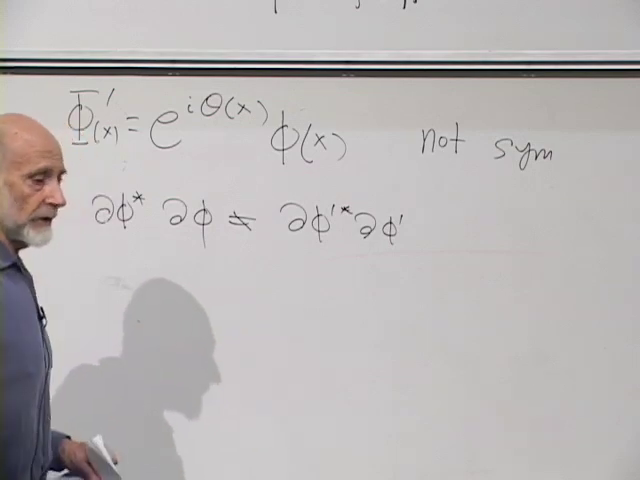
\includegraphics[width=0.78\textwidth]{lecture_08_figure_04.png}
\caption{Bảng ghi lại phép biến đổi pha cục bộ và việc
hạng đạo hàm thông thường không còn bất biến.}
\lectureframe{00:46:49}
\label{fig:l08-local-not-symmetry}
\end{figure}

Đưa vào một thế vectơ và cố định nhất quán một quy ước:
\begin{equation}
  D_\mu=\partial_\mu+i g A_\mu,
  \qquad
  A_\mu'=A_\mu-\frac1g\partial_\mu\theta.
  \label{eq:l08-covariant-convention}
\end{equation}
Khi đó
\begin{align}
  D_\mu'\phi'
  &=
  \left(\partial_\mu+i g A_\mu'\right)
  e^{i\theta}\phi
  \notag\\
  &=
  e^{i\theta}
  \left[
    \partial_\mu\phi+i(\partial_\mu\theta)\phi
    +i g A_\mu\phi-i(\partial_\mu\theta)\phi
  \right]
  \notag\\
  &=e^{i\theta}D_\mu\phi.
  \label{eq:l08-covariant-transform}
\end{align}
Các hạng không mong muốn triệt tiêu nhau. Đạo hàm liên hợp là
\begin{equation}
  (D_\mu\phi)^*
  =(\partial_\mu-i g A_\mu)\phi^*,
\end{equation}
và pha đối dấu của nó triệt tiêu trong tích
\begin{equation}
  (D_\mu\phi)^*D^\mu\phi.
\end{equation}

\begin{classroomqa}
\audiencequestion{Trong bài giảng trước, phép biến đổi của trường chuẩn có phải đã được viết với dấu ngược lại không?\lecturetimestamp{00:48:04}}
\lecturerresponse{Việc đồng thời đảo dấu trong \(D_\mu\) và trong
luật biến đổi chỉ là một quy ước. Với
\(D_\mu=\partial_\mu+i gA_\mu\) và
\(\phi'=e^{i\theta}\phi\), tính nhất quán đòi hỏi
\(A_\mu'=A_\mu-g^{-1}\partial_\mu\theta\). Quy ước thay thế cũng hoạt động
tốt như nhau nếu mọi dấu đều được đổi cùng nhau.}
\end{classroomqa}

\begin{classroomqa}
\audiencequestion{Việc dùng dạng viết hoa hay viết thường của
\(\phi\) trên bảng có đánh dấu một trường khác không?\lecturetimestamp{00:55:02}}
\lecturerresponse{Không có sự phân biệt nào được hàm ý. Hình dạng chữ thay đổi là do
cách viết tay, không phải một phép toán bổ sung hay một vô hướng thứ hai. Những phân biệt
có ý nghĩa là dấu prime, dấu sao liên hợp phức và chỉ số không-thời gian.}
\end{classroomqa}

\begin{classroomqa}
\audiencequestion{Liên hợp phức có phải là cùng một phép toán với việc nâng hoặc
hạ chỉ số Lorentz trong hạng động năng không?
\lecturetimestamp{00:56:50}}
\lecturerresponse{Không. Dấu sao liên hợp trường phức nội tại.
Các chỉ số Lorentz được nâng bằng metric không-thời gian:
\(D^\mu=g^{\mu\nu}D_\nu\). Một vô hướng Lorentz cần phép co
\((D_\mu\phi)^*D^\mu\phi\); cả hai phép toán đều có mặt và phục vụ những
mục đích khác nhau.}
\end{classroomqa}

\subsection{Trường chuẩn có động lực học riêng}

Cường độ trường
\begin{equation}
  F_{\mu\nu}=\partial_\mu A_\nu-\partial_\nu A_\mu
  \label{eq:l08-field-strength}
\end{equation}
là bất biến chuẩn vì hai đạo hàm bậc hai hỗn hợp của \(\theta\)
triệt tiêu nhau. Các thành phần thời gian--không gian của nó chứa điện trường, còn các
thành phần không gian--không gian chứa từ trường. Vì vậy điện động lực học vô hướng có dạng
\begin{equation}
  \mathcal L
  =(D_\mu\phi)^*D^\mu\phi
  -V(\phi^*\phi)
  -\frac14F_{\mu\nu}F^{\mu\nu}.
  \label{eq:l08-abelian-higgs}
\end{equation}
Trường mang điện ở đây là boson. Nó không phải trường electron, vốn là một
fermion. Một hạt nhân heli mang điện hoặc một ngưng tụ cặp Cooper minh họa
cách một bậc tự do boson mang điện có thể xuất hiện.

Trước khi phá vỡ đối xứng, hạng của trường chuẩn chứa các đạo hàm của \(A_\mu\)
nhưng không có hạng khối lượng trực tiếp. Ta có thể thử thêm
\begin{equation}
  \frac12m_A^2A_\mu A^\mu,
\end{equation}
nhưng dưới phép biến đổi trong Eq.~\eqref{eq:l08-covariant-convention},
\begin{equation}
  A_\mu A^\mu
  \longmapsto
  \left(A_\mu-\frac1g\partial_\mu\theta\right)
  \left(A^\mu-\frac1g\partial^\mu\theta\right),
  \label{eq:l08-bare-mass-fails}
\end{equation}
điều này không bằng \(A_\mu A^\mu\). Khối lượng trần của boson chuẩn bị cấm
bởi đối xứng cục bộ.

\begin{figure}[htbp]
\centering
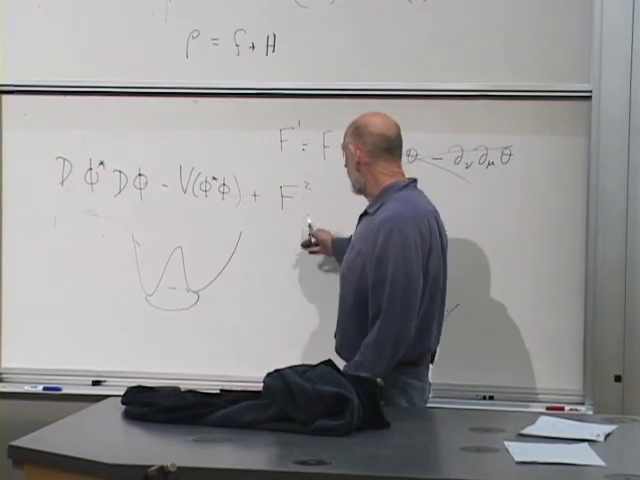
\includegraphics[width=0.76\textwidth]{lecture_08_figure_05.png}
\caption{Một trạng thái bảng đã được kiểm chứng cho thấy sự cản trở này: dưới một phép biến đổi chuẩn,
\(A_\mu A^\mu\) trở thành một bình phương có chứa
\(\partial_\mu\theta\), nên một khối lượng vectơ trần không bất biến.}
\lectureframe{01:07:30}
\label{fig:l08-bare-mass-board}
\end{figure}

\section{Cơ chế Higgs}

\subsection{Đạo hàm hiệp biến sinh ra khối lượng}

Quay lại thế bị phá vỡ và dùng tham số hóa được chuẩn hóa
chính tắc
\begin{equation}
  \phi(x)=\frac{f+h(x)}{\sqrt2}
  e^{i\pi(x)/f}.
\end{equation}
Đạo hàm hiệp biến của nó là
\begin{equation}
  D_\mu\phi
  =
  \frac{e^{i\pi/f}}{\sqrt2}
  \left[
    \partial_\mu h
    +i(f+h)
      \left(\frac{\partial_\mu\pi}{f}+gA_\mu\right)
  \right].
  \label{eq:l08-covariant-polar}
\end{equation}
Do đó,
\begin{equation}
\begin{aligned}
  (D_\mu\phi)^*D^\mu\phi
  ={}&
  \frac12(\partial_\mu h)^2
  \\
  &+\frac12(f+h)^2
    \left(\frac{\partial_\mu\pi}{f}+gA_\mu\right)
  \\
  &\hspace{4.2em}\times
    \left(\frac{\partial^\mu\pi}{f}+gA^\mu\right).
\end{aligned}
  \label{eq:l08-higgs-kinetic}
\end{equation}

Hạng quyết định xuất hiện trước bất kỳ lựa chọn chuẩn nào:
\begin{equation}
  \frac12g^2f^2 A_\mu A^\mu.
  \label{eq:l08-vector-mass-term}
\end{equation}
So sánh nó với dạng Proca
\(\frac12m_A^2A_\mu A^\mu\), ta được
\begin{equation}
  \boxed{m_A=g f}.
  \label{eq:l08-vector-mass}
\end{equation}
Khai triển này cũng sinh ra các tương tác
\(g^2fh A_\mu A^\mu\) và
\(\frac12g^2h^2A_\mu A^\mu\). Vì vậy khối lượng vectơ không phải là một sự
vi phạm đối xứng chuẩn tùy tiện. Nó xuất phát từ một hạng động năng vô hướng
bất biến chuẩn được xét trong một pha có độ lớn cân bằng khác không \(f\).

\begin{figure}[htbp]
\centering
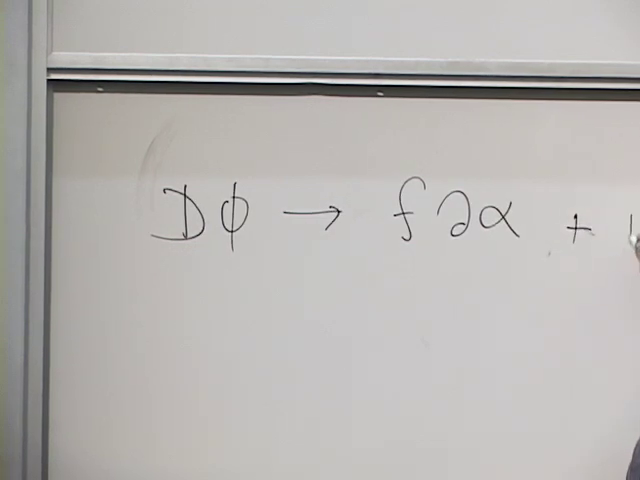
\includegraphics[width=0.78\textwidth]{lecture_08_figure_06.png}
\caption{Trên bảng, phần đóng góp \(f^2A^2\) được tách riêng trong
\((D\phi)^*(D\phi)\). Các hệ số số học phụ thuộc vào cách chuẩn hóa trường vô hướng và
hằng ghép chuẩn; với các Eq.~\eqref{eq:l08-canonical-polar}
và \eqref{eq:l08-covariant-convention}, kết quả là \(m_A=gf\).}
\lectureframe{01:10:10}
\label{fig:l08-generated-mass-board}
\end{figure}

Bài giảng hấp thụ \(g\) và một số hệ số \(\sqrt2\) vào kí hiệu trên bảng
của mình, nên trong lúc xác định khối lượng nó luân phiên trong chốc lát giữa \(f\), \(2f\) và \(\sqrt2f\).
Những hệ số ấy không có ý nghĩa bất biến cho đến khi cách chuẩn hóa
động năng và thế năng được nêu rõ. Kết quả bền vững là
\(m_A\propto gf\); Eq.~\eqref{eq:l08-vector-mass} cho hệ số đối với
quy ước được dùng ở đây.

\subsection{Pha được hấp thụ}

Dưới một phép biến đổi chuẩn, biến pha biến đổi theo
\begin{equation}
  \pi'(x)=\pi(x)+f\,\theta(x).
\end{equation}
Chọn
\begin{equation}
  \theta(x)=-\frac{\pi(x)}{f}.
  \label{eq:l08-unitary-gauge-choice}
\end{equation}
Khi đó \(\pi'=0\). Đây là chuẩn đơn nhất, trong đó
\begin{equation}
  \phi'(x)=\frac{f+h(x)}{\sqrt2}
\end{equation}
là thực, và Eq.~\eqref{eq:l08-higgs-kinetic} rút gọn thành
\begin{equation}
  (D_\mu\phi')^*D^\mu\phi'
  =
  \frac12(\partial_\mu h)^2
  +\frac12g^2(f+h)^2A_\mu'A^{\prime\mu}.
  \label{eq:l08-unitary-gauge-lagrangian}
\end{equation}
Trường Goldstone góc đã biến mất khỏi danh sách các biến độc lập,
trong khi khối lượng vectơ vẫn còn.

Trong bài giảng, điều này trước hết được minh họa trong giới hạn năng lượng thấp
\(\rho=f\), khi đó
\begin{align}
  \phi&=f e^{i\alpha},
  \notag\\
  D_\mu\phi
  &=if e^{i\alpha}
    \left(\partial_\mu\alpha+gA_\mu\right),
  \notag\\
  (D_\mu\phi)^*
  &=-if e^{-i\alpha}
    \left(\partial_\mu\alpha+gA_\mu\right).
  \label{eq:l08-frozen-radius}
\end{align}
Tích của chúng là
\begin{equation}
  f^2
  \left(\partial_\mu\alpha+gA_\mu\right)
  \left(\partial^\mu\alpha+gA^\mu\right).
\end{equation}
Chọn \(\theta=-\alpha\) thì còn lại \(g^2f^2A_\mu'A^{\prime\mu}\).

\begin{figure}[htbp]
\centering
\includegraphics[width=0.82\textwidth]{lecture_08_figure_07.png}
\caption{Trạng thái bảng đầy đủ khi bán kính bị cố định: các đạo hàm hiệp biến
chứa đồng thời đạo hàm pha và thế vectơ. Tiếp theo bài giảng
chọn \(\theta=-\alpha\), loại bỏ pha và để lại hạng khối lượng vectơ.}
\lectureframe{01:16:20}
\label{fig:l08-frozen-radius-board}
\end{figure}

\begin{classroomqa}
\audiencequestion{Có thể viết lại toàn bộ Lagrangian theo các biến làm cho
sự biến mất của mode góc trở nên hiển nhiên không?
\lecturetimestamp{01:13:49}}
\lecturerresponse{Có. Trong các biến cực, pha chỉ xuất hiện thông qua tổ hợp
bất biến chuẩn
\(\partial_\mu\alpha+gA_\mu\). Một phép biến đổi chuẩn với
\(\theta=-\alpha\) đặt pha bằng 0 ở mọi nơi mà chuẩn này được
xác định tốt. Khi đó hạng động năng vô hướng trở thành hạng khối lượng vectơ, còn
hạng cường độ trường bất biến chuẩn thì không đổi.}
\end{classroomqa}

\begin{classroomqa}
\audiencequestion{Các dao động của \(\alpha\) có không thể phân biệt được với các
dao động chuẩn không?\lecturetimestamp{01:18:02}}
\lecturerresponse{Trong lý thuyết có chuẩn, một biến thiên thuần túy của \(\alpha\) được
bù bởi biến thiên tương ứng của \(A_\mu\) là một sự mô tả lại theo chuẩn,
không phải một sóng vật lý riêng biệt. Đại lượng bất biến là
\(\partial_\mu\alpha+gA_\mu\). Mode vật lý từng được biểu diễn bởi trường Goldstone
toàn cục xuất hiện trở lại dưới dạng phân cực dọc của vectơ có
khối lượng.}
\end{classroomqa}

Người ta thường nói rằng một đối xứng chuẩn cục bộ bị phá vỡ tự phát.
Về mặt thao tác, cách nói này hữu ích: sau khi chọn một chuẩn, trường
vô hướng có giá trị chân không khác không và phổ chứa một vectơ có khối lượng.
Tuy nhiên, nói một cách chặt chẽ, các phép biến đổi chuẩn liên hệ những mô tả
dư thừa, chứ không phải những trạng thái vật lý khác biệt.
\editorialnote{Một sự dư thừa chuẩn cục bộ không bị phá vỡ theo cùng nghĩa
bất biến chuẩn như một đối xứng toàn cục. Phát biểu chính xác là lý thuyết
đang ở trong một pha Higgs. Lý thuyết nhiễu loạn sau khi cố định chuẩn mô tả
pha đó bằng một giá trị kỳ vọng khác không của trường vô hướng và phổ vectơ có khối lượng tương ứng.}

\section{Bậc tự do Goldstone đã đi đâu}

Không có gì vật lý có thể biến mất chỉ vì ta đổi biến. Hãy đếm các
bậc tự do trước và sau khi đi vào pha Higgs.

Trước đó:
\begin{equation}
  \underbrace{2}_{\text{massless vector}}
  +
  \underbrace{2}_{\text{complex scalar}}
  =4.
\end{equation}
Một vectơ không khối lượng có hai phân cực ngang. Vô hướng phức có
hai thành phần thực, hướng kính và góc.

Sau đó:
\begin{equation}
  \underbrace{3}_{\text{massive vector}}
  +
  \underbrace{1}_{\text{radial Higgs}}
  =4.
  \label{eq:l08-degree-count}
\end{equation}
Một vectơ có khối lượng có thể được đưa về trạng thái nghỉ. Trong hệ quy chiếu nghỉ
của nó không có hướng không gian nào được ưu tiên, nên nó phải có ba trạng thái
phân cực. Khi chuyển động, hai trạng thái là ngang và một trạng thái là dọc. Mode
Goldstone đã trở thành phân cực dọc đó.

\begin{figure}[htbp]
\centering
\begin{adjustbox}{max width=\linewidth}
\begin{tikzpicture}[x=1cm,y=1cm]
  \node[draw,rounded corners,fill=blue!7,minimum width=4.3cm,
        minimum height=2.1cm,align=center] (before) at (0,0)
    {massless \(A_\mu\): \(2\) transverse\\
     \(+\)\\
     complex \(\phi\): \(h+\pi\)};
  \node[draw,rounded corners,fill=orange!10,minimum width=4.3cm,
        minimum height=2.1cm,align=center] (after) at (7,0)
    {massive \(A_\mu\): \(2\) transverse\\
     \(+\;1\) longitudinal\\
     \(+\) radial \(h\)};
  \draw[->,very thick] (before) -- node[above]{Higgs phase} (after);
  \draw[->,teal!70!black,thick]
    (-0.15,-0.65) to[bend right=28]
    node[below,align=center]{Goldstone \(\pi\) supplies\\longitudinal mode}
    (6.8,-0.65);
\end{tikzpicture}
\end{adjustbox}
\caption{Cơ chế Higgs sắp xếp lại, chứ không phá hủy, các bậc tự do
vật lý.}
\label{fig:l08-degree-rearrangement}
\end{figure}

\begin{classroomqa}
\audiencequestion{Làm sao bậc tự do góc có thể biến mất mà không
vi phạm phép đếm bậc tự do?\lecturetimestamp{01:19:13}}
\lecturerresponse{Nó không biến mất về mặt vật lý. Một vectơ không khối lượng có
hai helicity vì không thể đưa nó về trạng thái nghỉ. Một vectơ có khối lượng có
ba phân cực, gồm cả một phân cực dọc. Mode Goldstone trở thành
phân cực thứ ba đó, nên tổng số không đổi.}
\end{classroomqa}

Bài giảng đưa ra một phép kiểm tra động học hữu ích. Hãy hình dung một hạt vectơ có
khối lượng, làm chậm nó về trạng thái nghỉ, rồi tăng tốc nó theo một hướng mới.
Một phân cực từng là ngang đối với chuyển động ban đầu có thể trở thành dọc so với
chuyển động mới. Tương tự, nếu một hạt có khối lượng phân cực tròn được đưa qua
trạng thái nghỉ rồi cho chuyển động theo hướng ngược lại, nhãn helicity của nó sẽ
đảo ngược. Một hạt thực sự không khối lượng không thể được đưa qua thí nghiệm này,
vì không có hệ quy chiếu quán tính nào có thể đưa nó về trạng thái nghỉ. Do đó hai
helicity của nó tạo thành một phổ vật lý nhất quán.

\section{Phép tương tự trong siêu dẫn}

Trong một chất siêu dẫn thông thường, các electron tạo thành các cặp Cooper. Một cặp là một
boson mang điện tích \(2e\), và chất ngưng tụ được mô tả bởi một
tham số trật tự phức mang điện. Khi độ lớn của nó khác không,
tổ hợp giữa pha của nó và thế vectơ điện từ tạo ra
cơ chế Anderson--Higgs. Từ trường tĩnh suy giảm trên độ xuyên sâu London
thay vì kéo dài tự do xuyên qua phần khối. Theo nghĩa chính xác phụ thuộc môi trường này,
photon hành xử như thể nó đã thu được khối lượng.

Ví dụ này cũng làm sáng tỏ sự phân biệt ở phần mở đầu. Trường điện từ
không bị chuyển hóa vĩnh viễn thành một hạt cơ bản khác.
Quy luật lan truyền có khối lượng thuộc về trạng thái tập thể bên trong vật liệu;
ở bên ngoài, photon chân không vẫn không khối lượng.

\section{Những gì đã được xác lập}

Giờ đây có thể cô đọng lập luận mà không làm mất logic của nó:
\begin{enumerate}
  \item Một đối xứng liên tục toàn cục bị phá vỡ có một phương góc phẳng và
        do đó có một mode Goldstone không khối lượng.
  \item Tính bất biến pha cục bộ đòi hỏi một thế chuẩn và thay
        \(\partial_\mu\) bằng \(D_\mu\).
  \item Một hạng khối lượng trần \(A_\mu A^\mu\) vi phạm luật biến đổi cục bộ.
  \item Khi vô hướng mang điện có độ lớn cân bằng khác không \(f\), hạng
        bất biến chuẩn \(|D_\mu\phi|^2\) chứa
        \(\frac12g^2f^2A_\mu A^\mu\).
  \item Pha có thể bị loại bỏ bằng một lựa chọn chuẩn, và bậc tự do vật lý
        của nó trở thành phân cực dọc của vectơ có khối lượng.
  \item Kích thích Higgs hướng kính còn lại, với khối lượng được ấn định bởi độ cong
        của thế vô hướng.
\end{enumerate}

Nhiệm vụ tiếp theo là cho fermion khối lượng. Electron và quark không thể
trực tiếp dùng cơ chế vectơ; các ghép Higgs của chúng là những
tương tác Yukawa. Một khi vô hướng ổn định tại \(f\), các tương tác ấy trở thành
các hạng khối lượng fermion.

Phát biểu khái quát rằng các hạt quen thuộc sẽ không khối lượng nếu không có
sự phá vỡ đối xứng điện yếu cần thêm một điều lưu ý cuối cùng. Khối lượng
của các quark cơ bản và các lepton mang điện, cũng như khối lượng của \(W\) và \(Z\),
quả thật biến mất cùng với giá trị kỳ vọng Higgs. Tuy nhiên, phần lớn khối lượng của proton và neutron
phát sinh một cách động từ sự giam hãm QCD và năng lượng trường mạnh, chứ không phải từ khối lượng Higgs của các quark. Sự phân biệt đó không
làm thay đổi cơ chế Higgs được suy ra ở đây; nó giữ cho miền áp dụng của cơ chế ấy được chính xác.

\chapter{Khối lượng fermion: chirality, các tương tác Yukawa và neutrino Majorana}

\lectureoverview{Trước hết ta dựng lại cơ chế Higgs của boson chuẩn trong một lý thuyết mô hình đồ chơi \(U(1)\), rồi đặt câu hỏi song song đối với fermion. Khối lượng Dirac trộn các trường chiral trái và phải, nhưng tương tác yếu gán cho chúng các điện tích khác nhau và vì thế cấm một khối lượng trần. Một tương tác Yukawa với trường Higgs tôn trọng đối xứng; sau khi trường Higgs nhận một giá trị chân không, chính tương tác đó trở thành khối lượng fermion và một liên kết Higgs--fermion đo được. Phần cuối đi theo logic này sang khối lượng neutrino, các hạt nặng khả dĩ không được bảo vệ, động học tia vũ trụ, quán tính tương đối tính và hấp dẫn.}

Mục đích của phần ôn mở đầu không chỉ đơn thuần là lặp lại bài giảng trước. Ta cần một ý từ đó ở dạng có thể chuyển sang cho fermion: khối lượng là năng lượng khác không của một kích thích tại xung lượng bằng không. Đối với một trường, xung lượng bằng không nghĩa là bước sóng vô hạn, hay một độ dời như nhau ở mọi nơi. Một lý thuyết chỉ có đạo hàm không thể phát hiện một độ dời đồng nhất. Một số hạng không có đạo hàm thì có thể.

\section{Câu chuyện boson chuẩn trong một lượt}

\subsection{Năng lượng đạo hàm và một vectơ không khối lượng}

Trường chuẩn mô hình là \(A_\mu\), với cường độ trường
\begin{equation}
  F_{\mu\nu}
  =\partial_\mu A_\nu-\partial_\nu A_\mu .
  \label{eq:l09-field-strength}
\end{equation}
Trên bảng, số hạng động học của trường chuẩn được viết một cách ký hiệu là \(F^2\). Với chuẩn hóa tiêu chuẩn, nó là
\begin{equation}
  \mathcal L_{\mathrm{gauge}}
  =-\frac14 F_{\mu\nu}F^{\mu\nu}.
  \label{eq:l09-gauge-kinetic}
\end{equation}

\begin{figure}[htbp]
\centering
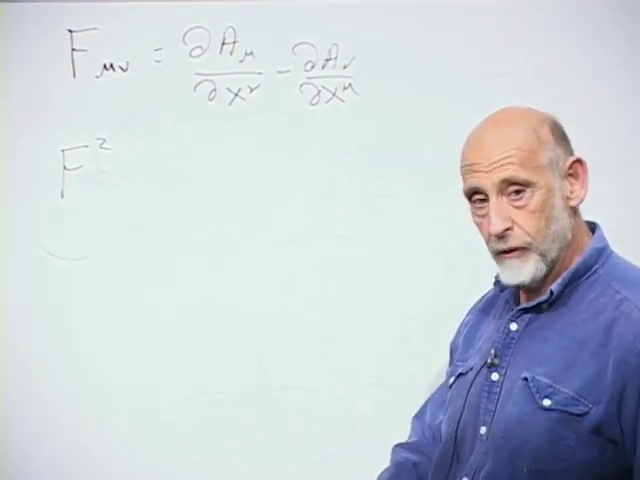
\includegraphics[width=0.72\textwidth]{lecture_09_figure_02.png}
\caption{Định nghĩa cường độ trường và ký hiệu tắt \(F^2\) trên bảng cho năng lượng đạo hàm của trường chuẩn.}
\lectureframe{00:02:39}
\label{fig:l09-field-strength-board}
\end{figure}

Mỗi lần \(A_\mu\) xuất hiện trong \eqref{eq:l09-gauge-kinetic} đều nằm dưới dấu đạo hàm. Vì vậy,
\begin{equation}
  A_\mu(x)\longmapsto A_\mu(x)+c_\mu,
  \qquad \partial_\nu c_\mu=0,
\end{equation}
không làm thay đổi \(F_{\mu\nu}\). Do đó, một thế vectơ đồng nhất không tốn năng lượng cường độ trường. Theo ngôn ngữ của bài giảng, mode xung lượng bằng không không có khe năng lượng và boson chuẩn là không khối lượng.

Trường \(U(1)\) này là một vật thay thế được cố ý làm đơn giản. Đích vật lý thực sự là \(W^\pm\) và \(Z\), chứ không phải photon điện từ. Đối xứng điện từ không bị phá vỡ giữ cho photon không khối lượng; đối xứng điện yếu bị phá vỡ trao khối lượng cho các boson chuẩn yếu.

\subsection{Đóng băng bán kính Higgs}

Hãy đưa vào một trường vô hướng phức mang điện và viết nó ở dạng cực,
\begin{equation}
  \phi(x)=\rho(x)e^{i\alpha(x)}.
\end{equation}
Thế mũ Mexico của nó đạt cực tiểu trên một đường tròn có bán kính khác không. Gọi bán kính ấy là \(f\), thì phương bán kính tương đối cứng. Trong lượt xét đầu tiên, ta đóng băng nó và chỉ giữ lại pha:
\begin{equation}
  \phi(x)\simeq f e^{i\alpha(x)}.
  \label{eq:l09-frozen-higgs}
\end{equation}

\begin{figure}[htbp]
\centering
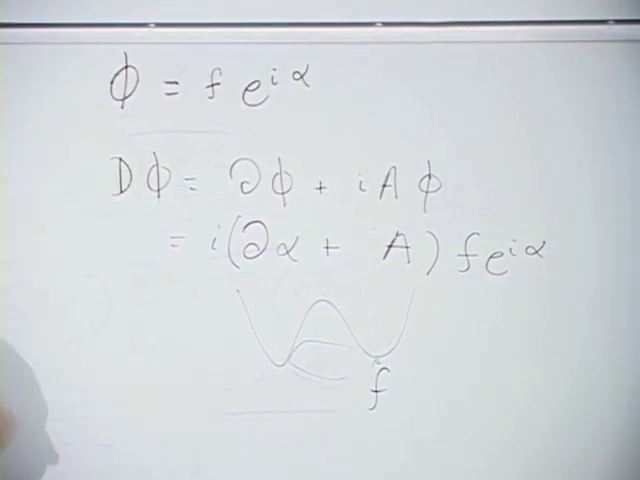
\includegraphics[width=0.72\textwidth]{lecture_09_figure_03.png}
\caption{Bán kính Higgs đã đóng băng, đạo hàm hiệp biến của nó và phác họa nhỏ của thế bị phá vỡ dùng trong phần ôn lại.}
\lectureframe{00:06:42}
\label{fig:l09-frozen-board}
\end{figure}

Chọn quy ước
\begin{equation}
\begin{aligned}
  D_\mu&=\partial_\mu+igA_\mu,
  \\
  \phi&\longmapsto e^{i\theta}\phi,
  \\
  A_\mu&\longmapsto A_\mu-\frac1g\partial_\mu\theta .
\end{aligned}
  \label{eq:l09-gauge-convention}
\end{equation}
Bài giảng ẩn \(g\) đi; giữ nó hiện ra làm cho thứ nguyên và khối lượng xuất hiện về sau trở nên rõ ràng. Tác dụng lên trường đã đóng băng cho
\begin{align}
  D_\mu\phi
  &=(\partial_\mu+igA_\mu)f e^{i\alpha}
  \notag\\
  &=i\bigl(\partial_\mu\alpha+gA_\mu\bigr)
    f e^{i\alpha}.
  \label{eq:l09-covariant-frozen}
\end{align}
Nhân với liên hợp phức loại bỏ pha, đồng thời cũng biến \(i\) nhân \(-i\) thành \(+1\):
\begin{equation}
  |D_\mu\phi|^2
  =f^2
   \bigl(\partial_\mu\alpha+gA_\mu\bigr)
   \bigl(\partial^\mu\alpha+gA^\mu\bigr).
  \label{eq:l09-frozen-square}
\end{equation}

\begin{classroomqa}
\audiencequestion{Bình phương của đạo hàm hiệp biến có nên mang dấu trừ vì đạo hàm tạo ra một thừa số \(i\) không?
\lecturetimestamp{00:07:39}}
\lecturerresponse{Không. Số hạng động học là tích với liên hợp phức. Một thừa số đóng góp \(i\), thừa số kia đóng góp \(-i\), và \(i(-i)=1\). Quy ước dấu cho \(D_\mu\) có thể được đảo một cách nhất quán, nhưng bình phương môđun là dương trong biểu thức năng lượng tương ứng.}
\end{classroomqa}

Tổ hợp trong \eqref{eq:l09-frozen-square} tự nó là một trường chuẩn đã bị dịch. Chọn \(\theta=-\alpha\), để pha của trường vô hướng biến mất, và định nghĩa
\begin{equation}
  A'_\mu=A_\mu+\frac1g\partial_\mu\alpha .
  \label{eq:l09-unitary-gauge-field}
\end{equation}
Khi đó
\begin{equation}
  |D_\mu\phi|^2=g^2f^2 A'_\mu A'^\mu .
  \label{eq:l09-vector-mass-term}
\end{equation}
Số hạng mới không chứa đạo hàm nào của \(A'_\mu\). Bây giờ một trường đồng nhất tích trữ năng lượng, nên mode vectơ xung lượng bằng không có khe năng lượng.

\begin{figure}[htbp]
\centering
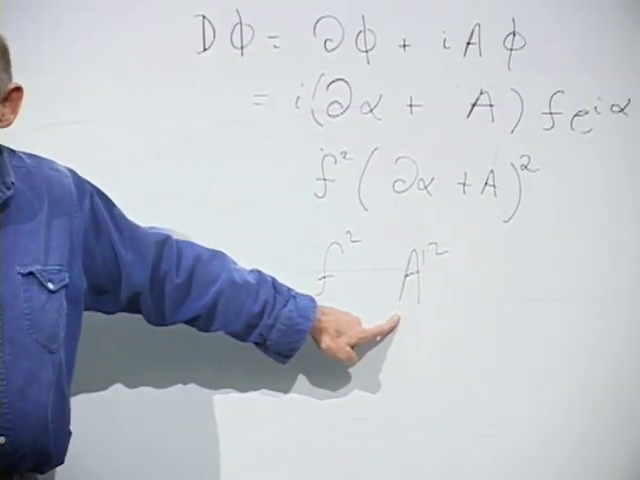
\includegraphics[width=0.72\textwidth]{lecture_09_figure_04.png}
\caption{Trên bảng tách riêng số hạng \(f^2A^2\), báo hiệu khối lượng của boson chuẩn sau khi pha đã được hấp thụ.}
\lectureframe{00:10:31}
\label{fig:l09-vector-mass-board}
\end{figure}

Với chuẩn hóa chuẩn tắc của trường vô hướng, ta viết
\(\phi=(f+h)e^{i\pi/f}/\sqrt2\). So sánh số hạng vectơ thu được với
\(\tfrac12m_A^2A_\mu A^\mu\) cho
\begin{equation}
  m_A=gf
  \label{eq:l09-abelian-vector-mass}
\end{equation}
trong mô hình abel này. Bài giảng ẩn các hệ số chuẩn hóa đi và tóm tắt kết quả bằng cách nói rằng khối lượng vectơ được quyết định bởi \(f\).

Mode pha không biến mất mà không được tính đến. Trước khi đối xứng được chuẩn hóa, nó là một boson Goldstone không khối lượng. Sau khi chuẩn hóa, nó cung cấp phân cực dọc cần thiết cho một hạt vectơ có khối lượng. Dao động theo phương bán kính, thứ mà ta tạm thời đã đóng băng, còn lại như kích thích Higgs vật lý.

\subsection{Vì sao một số hạng không có đạo hàm lại có nghĩa là khối lượng}

\begin{classroomqa}
\audiencequestion{Vì sao một số hạng \(A'^2\) lại được tính là khối lượng chứ không chỉ là một tương tác khác?\lecturetimestamp{00:13:10}}
\lecturerresponse{Khối lượng là năng lượng khi đứng yên. Đối với một trường, một hạt đứng yên là lượng tử của một mode xung lượng bằng không, bước sóng vô hạn. Số hạng đạo hàm không cho năng lượng đối với một độ dời đồng nhất tĩnh, còn \(m_A^2A'^2\) thì có. Năng lượng xung lượng bằng không khác không ấy chính là khe năng lượng nghỉ.}
\end{classroomqa}

Bài giảng triển khai phát biểu này qua ba phép loại suy cơ học.

\begin{itemize}
  \item Trong một tinh thể, một độ dời biến thiên chậm tốn năng lượng đàn hồi vì các nguyên tử lân cận bị dịch đi khác nhau. Một phép tịnh tiến cứng dịch chuyển mọi nguyên tử cùng nhau và không tốn nội năng. Vì vậy phonon âm không có khe năng lượng.
  \item Trong một nam châm lý tưởng đối xứng quay, một phương spin biến thiên theo không gian tốn năng lượng trao đổi, nhưng quay mọi spin cùng nhau thì không. Sóng spin bước sóng dài liên hệ với nó vì thế không có khe năng lượng.
  \item Trong một plasma, dịch chuyển chất lỏng electron so với nền dương tạo ra sự tách điện tích và một điện trường phục hồi ngay cả đối với một độ dời tương đối đồng nhất. Plasmon kết quả có tần số khác không tại số sóng bằng không.
\end{itemize}

Trường chuẩn đã Higgs hóa cư xử giống ví dụ thứ ba: môi trường bị phá vỡ chống lại điều mà nếu không thì sẽ là một độ dời đồng nhất không tốn năng lượng.

\begin{classroomqa}
\audiencequestion{Trước khi đưa trường chuẩn vào, pha \(\alpha\) chẳng phải đã dao động rồi sao?\lecturetimestamp{00:18:24}}
\lecturerresponse{Đúng vậy. Năng lượng của nó tỉ lệ với
\(f^2(\partial_\mu\alpha)^2\). Một pha biến thiên từ nơi này sang nơi khác có năng lượng gradient và có thể lan truyền, nhưng một thay đổi pha đồng nhất thì không tốn gì. Đó chính xác là mode Goldstone không khối lượng.}
\end{classroomqa}

\begin{classroomqa}
\audiencequestion{Đạo hàm có bao gồm đạo hàm theo thời gian. Việc thực sự làm chuyển động cả mạng tinh thể hoặc làm thay đổi toàn bộ trường chẳng phải vẫn mang năng lượng động học sao?\lecturetimestamp{00:22:18}}
\lecturerresponse{Có. Sự so sánh ở đây là giữa các cấu hình tĩnh, hoặc giữa các cấu hình được chuẩn bị chậm tùy ý. Một mạng tinh thể tịnh tiến với vận tốc khác không có năng lượng động học. Phép kiểm tra khối lượng hỏi xem cấu hình ấy có còn năng lượng khi nó đứng yên và đồng nhất trong không gian hay không.}
\end{classroomqa}

\section{Manh mối thực nghiệm: tương tác yếu phân biệt trái và phải}

Bây giờ bài giảng chuyển sang electron, muon và quark. Khối lượng của chúng cũng đến từ trường Higgs, nhưng cơ chế trông khác đi vì khối lượng fermion không phải là một số hạng vectơ bậc hai. Nó là một liên kết giữa hai trường chiral.

\subsection{Vi phạm đối xứng chẵn lẻ trong phân rã beta}

Bắt đầu từ sự kiện thực nghiệm rằng tương tác yếu vi phạm đối xứng chẵn lẻ. Điện động lực học lượng tử và sắc động lực học lượng tử đối xử như nhau với một quá trình và ảnh gương của nó. Tương tác yếu thì không. Trong phân rã beta của neutron,
\begin{equation}
  n\longrightarrow p+e^-+\bar\nu_e,
  \label{eq:l09-beta-decay}
\end{equation}
những electron năng lượng cao được tương tác dòng mang điện chọn lọc có helicity trái: spin của chúng hướng ngược với xung lượng. Các phản neutrino tương ứng có helicity ngược lại.

Đối với một hạt siêu tương đối tính, định nghĩa helicity bằng
\begin{equation}
  h=\frac{\bm S\cdot\bm p}{|\bm S|\,|\bm p|}.
\end{equation}
Spin song song với xung lượng có \(h=+1\); spin ngược song song có \(h=-1\). Tương tác yếu ghép với một trường electron chiral trái và một trường neutrino chiral trái, chứ không ghép với một trường electron chiral phải theo cùng cách đó.\editorialnote{Ban đầu bài giảng dùng tính tay theo nghĩa helicity vì điều đó trực quan về mặt hình dung ở năng lượng cao. Các điện tích chuẩn thực sự tác dụng lên chirality, nhãn biểu diễn Lorentz được chọn bởi \(P_L=(1-\gamma^5)/2\) và \(P_R=(1+\gamma^5)/2\). Đối với một hạt không khối lượng, chirality và helicity trùng nhau đối với hạt; đối với một hạt có khối lượng thì chúng không trùng nhau.}

Để làm lộ ra chướng ngại này mà không cần toàn bộ phần hạch toán \(SU(2)_L\times U(1)_Y\), hãy tưởng tượng một thế giới \(U(1)\) giả trong đó chỉ \(\psi_L\) mang điện tích liên quan:
\begin{equation}
  \psi_L\longmapsto e^{i\theta}\psi_L,
  \qquad
  \psi_R\longmapsto\psi_R .
  \label{eq:l09-chiral-toy-charge}
\end{equation}
Đây không phải điện từ học: các electron chiral trái và chiral phải thực sự mang cùng điện tích điện. Nó là một bức biếm họa của tương tác yếu, trong đó hai chirality nằm trong các biểu diễn điện yếu khác nhau.

\begin{classroomqa}
\audiencequestion{Sự bất đối xứng trái--phải ấy có áp dụng tương tự cho quark không?
\lecturetimestamp{00:31:50}}
\lecturerresponse{Có, với các đa tuyến yếu và hypercharge thích hợp. Các quark chiral trái kiểu up và kiểu down tạo thành các doublet yếu, còn các trường chiral phải là các singlet yếu. Vì vậy, các liên kết Higgs của chúng cũng đối mặt với cùng một vấn đề cấu trúc như của electron.}
\end{classroomqa}

\section{Khối lượng Dirac là sự trộn trái--phải}

\subsection{Từ phương trình bốn thành phần đến hai phương trình Weyl}

Một hàm sóng Dirac có bốn thành phần. Nói một cách lỏng lẻo, hai thành phần mô tả spin và hai thành phần phân biệt các nghiệm năng lượng dương và năng lượng âm, trong đó các nghiệm sau được diễn giải lại như các bậc tự do phản hạt. Ở dạng Hamilton,
\begin{equation}
  i\frac{\partial\Psi}{\partial t}
  =\left(-i\bm\alpha\cdot\bm\nabla+m\beta\right)\Psi .
  \label{eq:l09-dirac-hamiltonian}
\end{equation}
Các ma trận \(\alpha_i\) và \(\beta\) mã hóa quan hệ tương đối tính giữa năng lượng, xung lượng và khối lượng.

\begin{figure}[htbp]
\centering
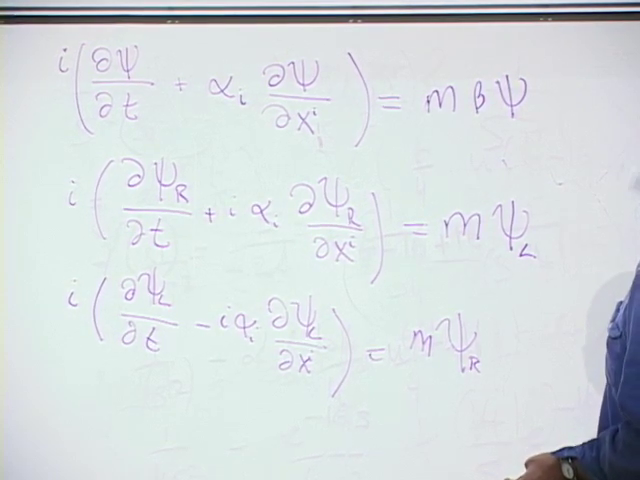
\includegraphics[width=0.74\textwidth]{lecture_09_figure_05.png}
\caption{Trên bảng trước hết viết phương trình Dirac, rồi tách nó thành các phương trình tay trái và tay phải ghép cặp với nhau.}
\lectureframe{00:40:30}
\label{fig:l09-dirac-board}
\end{figure}

Cơ sở chiral làm cho vai trò của \(m\) trở nên tường minh. Với
\(\sigma^\mu=(1,\bm\sigma)\) và
\(\bar\sigma^\mu=(1,-\bm\sigma)\),
\begin{align}
  i\bar\sigma^\mu\partial_\mu\psi_L&=m\psi_R,
  \label{eq:l09-weyl-left}\\
  i\sigma^\mu\partial_\mu\psi_R&=m\psi_L.
  \label{eq:l09-weyl-right}
\end{align}
Khi \(m=0\), các phương trình độc lập: một trường chiral trái và một trường chiral phải có thể lan truyền mà không ghép với nhau. Khi \(m\neq0\), mỗi trường xuất hiện như nguồn của trường kia. Đó là nghĩa chính xác mà theo đó một khối lượng Dirac trộn trái và phải.

Susskind mô tả điều này như fermion dao động giữa trái và phải. Lối nói ấy nắm bắt được sự ghép, nhưng không nên đẩy nó thành một bức tranh cổ điển theo nghĩa đen về một hạt điểm lật qua lật lại. Phát biểu chính xác là hệ phương trình trường ghép
\eqref{eq:l09-weyl-left}--\eqref{eq:l09-weyl-right}.

\begin{classroomqa}
\audiencequestion{Các thừa số \(i\) và các dấu trong hai phương trình trên bảng có nhất quán không?\lecturetimestamp{00:41:10}}
\lecturerresponse{Nếu xét từng dòng trên bảng thì không; một \(i\) đã bị kéo ra ngoài một cách không nhất quán trong phép suy ra nhanh. Nội dung đáng tin cậy là mô thức ghép. Các phương trình \eqref{eq:l09-weyl-left} và
\eqref{eq:l09-weyl-right} cho một quy ước nhất quán tiêu chuẩn.}
\end{classroomqa}

\subsection{Vì sao đối xứng yếu cấm một khối lượng trần}

Số hạng khối lượng Dirac tương ứng trong Lagrangian là
\begin{equation}
  \mathcal L_m
  =-m\bar\psi\psi
  =-m\left(\bar\psi_L\psi_R+\bar\psi_R\psi_L\right).
  \label{eq:l09-bare-dirac-mass}
\end{equation}
Dưới phép biến đổi mô hình đồ chơi \eqref{eq:l09-chiral-toy-charge},
\begin{equation}
  \bar\psi_L\psi_R\longmapsto
  e^{-i\theta}\bar\psi_L\psi_R,
  \qquad
  \bar\psi_R\psi_L\longmapsto
  e^{i\theta}\bar\psi_R\psi_L.
\end{equation}
Không số hạng nào là bất biến. Vì vậy hệ số trộn trực tiếp trái--phải \(m\) bị cấm trước khi đối xứng bị phá vỡ.

Chỉ riêng điện từ học sẽ không gây ra vấn đề này, vì \(\psi_L\) và
\(\psi_R\) có cùng điện tích điện. Chướng ngại nảy sinh từ các số lượng tử yếu khác nhau của chúng.

\subsection{Các câu hỏi về helicity làm lộ ra sự tinh tế của chirality}

Bây giờ lớp học kiểm tra bức tranh trực giác về tính tay từ nhiều góc độ. Những câu hỏi này không phải chuyện bên lề: chúng chỉ ra chính xác helicity hữu ích ở đâu và ở đâu chirality phải thay thế nó.

\begin{classroomqa}
\audiencequestion{Thế giới sẽ ra sao nếu tương tác yếu phát ra electron với cả hai độ xoắn như nhau?\lecturetimestamp{00:42:12}}
\lecturerresponse{Sự bất đối xứng chẵn lẻ trực tiếp sẽ biến mất khỏi quá trình đó. Nhưng lý thuyết điện yếu thực sự là chiral: chỉ các bộ đôi chiral trái mới mang tương tác yếu mang điện. Bài giảng tạm hoãn một trình bày đầy đủ hơn về vì sao tự nhiên lại chọn cấu trúc đó.}
\end{classroomqa}

\begin{classroomqa}
\audiencequestion{Giả sử spin của một electron được chuẩn bị theo phương thẳng đứng và sau đó electron được gia tốc theo phương ngang. Nó là tay trái hay tay phải?
\lecturetimestamp{00:42:44}}
\lecturerresponse{Một trạng thái spin vuông góc với động lượng là chồng chập của hai độ xoắn. Độ xoắn chỉ xác định rõ khi spin song song hoặc phản song song với động lượng. Tuy vậy, các toán tử chiếu chiral yếu vẫn được xác định rõ cho trường.}
\end{classroomqa}

Một hạt có khối lượng có thể bị làm chậm đến đứng yên rồi được gia tốc theo hướng ngược lại mà không đảo spin của nó. Khi đó độ xoắn của nó đổi dấu. Một hạt không khối lượng không thể bị vượt qua hoặc bị đưa về trạng thái đứng yên bằng một phép boost Lorentz, nên độ xoắn của nó bất biến dưới các phép boost Lorentz riêng. Điều này thúc đẩy phát biểu trong bài giảng rằng một loại hạt chỉ có một độ xoắn vật lý thì phải không khối lượng. Phát biểu chính xác hơn trong lý thuyết trường là một hạng khối lượng Dirac bất biến Lorentz đòi hỏi cả hai thành phần chiral.

\begin{classroomqa}
\audiencequestion{Một photon phân cực tròn có thể phản xạ trên gương và đảo hướng mà không hề dừng lại. Điều đó có mâu thuẫn với lập luận về độ xoắn không?\lecturetimestamp{00:45:28}}
\lecturerresponse{Không. Gương là một hệ bên ngoài có thể trao đổi mômen góc và đảo hướng lan truyền. Một quá trình phản xạ không phải là một phép boost Lorentz vượt qua photon. Việc có tồn tại một kênh hay không còn phụ thuộc vào các trạng thái phân cực được phép và các điều kiện biên của vật liệu.}
\end{classroomqa}

\begin{classroomqa}
\audiencequestion{Một chùm electron thông thường chứa chỉ một loại thuận tay hay cả hai?\lecturetimestamp{00:46:10}}
\lecturerresponse{Nói chung là cả hai. Một trạng thái electron có khối lượng chứa cả hai thành phần chiral, và một chùm không phân cực chứa cả hai độ xoắn. Các nguồn chuyên dụng có thể tạo ra một chùm phân cực với bất đối xứng độ xoắn lớn.}
\end{classroomqa}

\begin{classroomqa}
\audiencequestion{Có thể hội tụ một chùm độc lập với spin của nó không, hay từ trường tách hai phân cực ra?\lecturetimestamp{00:46:29}}
\lecturerresponse{Việc hội tụ vị trí thông thường có thể phần lớn không nhạy với spin, nhưng mômen từ lại ghép với gradient từ trường. Vì vậy, các nguồn chọn lọc spin, các gradient kiểu Stern--Gerlach, và động lực học spin trong máy gia tốc có thể chuẩn bị hoặc tách các phân cực.}
\end{classroomqa}

\begin{classroomqa}
\audiencequestion{Sự khác biệt trong tương tác yếu giữa trái và phải có chỉ là ngẫu nhiên không?\lecturetimestamp{00:48:13}}
\lecturerresponse{Đối với học phần hiện tại, đó là một sự kiện thực nghiệm đã được đưa vào Mô hình Chuẩn. Nó quá có hệ thống để có cảm giác như một sự tình cờ đơn thuần, nhưng bản thân Mô hình Chuẩn không suy ra mẫu đầy đủ của các điện tích chiral từ một nguyên lý sâu hơn.}
\end{classroomqa}

\section{Xây dựng Yukawa}

\subsection{Để Higgs mang điện tích còn thiếu}

Đối xứng cấm một hạng khối lượng dạng số, nhưng nó cho phép một tương tác với một trường cung cấp pha biến đổi còn thiếu. Hãy đưa vào một trường vô hướng phức với
\begin{equation}
  \phi\longmapsto e^{i\theta}\phi,
  \qquad
  \phi^\dagger\longmapsto e^{-i\theta}\phi^\dagger.
  \label{eq:l09-scalar-charge}
\end{equation}
Khi đó
\begin{equation}
  \mathcal L_Y
  =-y\,\bar\psi_L\phi\psi_R
   -y^*\,\bar\psi_R\phi^\dagger\psi_L
  \label{eq:l09-yukawa-lagrangian}
\end{equation}
là bất biến chuẩn. Trong hạng thứ nhất,
\(\bar\psi_L\) đóng góp \(e^{-i\theta}\) và \(\phi\) đóng góp
\(e^{i\theta}\); các pha triệt tiêu nhau. Hạng thứ hai là liên hợp Hermite của hạng đó.

Tương đương, các phương trình chiral thu được sự trộn phụ thuộc vào trường:
\begin{align}
  i\bar\sigma^\mu D_\mu\psi_L
    &=y\phi\psi_R,
  \label{eq:l09-yukawa-eom-left}\\
  i\sigma^\mu\partial_\mu\psi_R
    &=y^*\phi^\dagger\psi_L.
  \label{eq:l09-yukawa-eom-right}
\end{align}

\begin{figure}[htbp]
\centering
\includegraphics[width=0.76\textwidth]{lecture_09_figure_06.png}
\caption{Khối lượng trần ở các vế phải đã được thay bằng trường vô hướng mang điện. Các dấu viết trên bảng chỉ có tính sơ đồ; cấu trúc bất biến được cho trong \eqref{eq:l09-yukawa-lagrangian}.}
\lectureframe{00:51:30}
\label{fig:l09-yukawa-board}
\end{figure}

Trước khi đối xứng bị phá vỡ, đây là một tương tác chứ không phải khối lượng. Một fermion chiral phải chỉ có thể trở thành một fermion chiral trái khi phát ra hoặc hấp thụ lượng tử của trường vô hướng cần thiết để cân bằng điện tích. Hệ số \(y\) là hằng số ghép Yukawa, không phải điện tích chuẩn \(g\).

\begin{classroomqa}
\audiencequestion{Có hợp lệ không nếu đơn giản đặt \(\phi\) và
\(\phi^\dagger\) vào vế phải của hai phương trình?
\lecturetimestamp{00:51:55}}
\lecturerresponse{Điều đó hợp lệ chính vì các pha biến đổi của chúng sửa chữa sự không khớp. Phép kiểm tra quyết định không phải là hình thức bề ngoài của phương trình mà là tính bất biến chuẩn của tương tác
\(\bar\psi_L\phi\psi_R+\mathrm{h.c.}\).}
\end{classroomqa}

\subsection{Chân không biến tương tác thành khối lượng}

Bây giờ hãy đồng nhất \(\phi\) với trường Higgs và cho nó ổn định ở một độ lớn chân không khác không. Theo chuẩn hoá đơn giản hoá của bài giảng,
\begin{equation}
  \phi\simeq f,
\end{equation}
nên \eqref{eq:l09-yukawa-lagrangian} chứa
\begin{equation}
  \mathcal L_Y
  \supset
  -yf\,\bar\psi_L\psi_R
  -y^*f\,\bar\psi_R\psi_L .
\end{equation}
Sau một phép tái định nghĩa pha vô hại, khi thích hợp, khối lượng fermion là
\begin{equation}
  m_f=yf.
  \label{eq:l09-lecture-fermion-mass}
\end{equation}
Đây là đối ứng fermion của kết quả vectơ \(m_A=gf\). Cùng một chân không Higgs vừa cung cấp một phân cực dọc cho các boson chuẩn yếu vừa cung cấp các số lượng tử yếu còn thiếu cần thiết để ghép các fermion trái và phải.

Trong quy ước Mô hình Chuẩn với chuẩn hoá chính tắc,
\begin{equation}
  H(x)=\frac1{\sqrt2}
  \begin{pmatrix}
    0\\ v+h(x)
  \end{pmatrix},
  \qquad v\simeq246\ \mathrm{GeV},
  \label{eq:l09-sm-higgs-vacuum}
\end{equation}
và do đó
\begin{equation}
  m_f=\frac{y_fv}{\sqrt2}.
  \label{eq:l09-sm-fermion-mass}
\end{equation}
\(f\) của bài giảng và \(v/\sqrt2\) theo quy ước chỉ khác nhau bởi lựa chọn chuẩn hoá này.

\begin{classroomqa}
\audiencequestion{Nếu chỉ tích \(yf\) mới là khối lượng fermion, thì làm sao có thể xác định riêng rẽ hằng số ghép \(y\) và thang chân không \(f\)?
\lecturetimestamp{00:55:36}}
\lecturerresponse{Khối lượng của các boson chuẩn yếu xác định thang chân không một khi các hằng số ghép chuẩn đã biết. Khi đó khối lượng đo được của một fermion xác định hằng số ghép Yukawa của nó. Trong lý thuyết đầy đủ,
\(m_W=gv/2\), \(m_Z=v\sqrt{g^2+g'^2}/2\), và
\(y_f=\sqrt2m_f/v\).}
\end{classroomqa}

\begin{classroomqa}
\audiencequestion{Khối lượng boson yếu có khoảng \(900\ \mathrm{GeV}\) không?
\lecturetimestamp{00:57:43}}
\lecturerresponse{Không; bài giảng ngay lập tức sửa chỗ lỡ lời đó thành xấp xỉ
\(90\ \mathrm{GeV}\). Chính xác hơn,
\(m_W\simeq80\ \mathrm{GeV}\) và \(m_Z\simeq91\ \mathrm{GeV}\), trong khi thang chân không nền tảng là \(v\simeq246\ \mathrm{GeV}\).}
\end{classroomqa}

\subsection{Một thang chân không, nhiều hằng số ghép Yukawa}

Mỗi loài fermion mang điện có hằng số ghép Yukawa riêng:
\begin{equation}
  m_i=y_i f
  \qquad\text{(lecture normalization)}.
  \label{eq:l09-mass-family}
\end{equation}

\begin{figure}[htbp]
\centering
\includegraphics[width=0.76\textwidth]{lecture_09_figure_08.png}
\caption{Trên bảng, sự phụ thuộc theo loài được tóm tắt thành \(m_i=g_i f\); các \(g_i\) viết ở đó chính là các hằng số ghép Yukawa được gọi là \(y_i\) ở đây.}
\lectureframe{01:16:30}
\label{fig:l09-mass-family-board}
\end{figure}

Đối với electron, bài giảng ước lượng
\begin{equation}
  y_e\sim\frac{0.5\ \mathrm{MeV}}{10^2\ \mathrm{GeV}}
  \sim10^{-5}.
\end{equation}
Dùng giá trị chính tắc \(v=246\ \mathrm{GeV}\) cho kết quả chính xác hơn là
\(y_e\simeq2.9\times10^{-6}\). Quark top nằm ở đầu đối diện:
\begin{equation}
  y_t=\frac{\sqrt2m_t}{v}\simeq1.
\end{equation}
Vì vậy, cơ chế Higgs giải thích bằng cách nào một khối lượng bất biến chuẩn có thể tồn tại, nhưng nó không giải thích được thứ bậc cực lớn giữa các \(y_i\). Các khối lượng fermion quan sát được chỉ đơn thuần chuyển thứ bậc đó thành các con số đo được.

\begin{classroomqa}
\audiencequestion{Quark top thực sự có hằng số ghép Yukawa cỡ 1 sao?\lecturetimestamp{00:59:09}}
\lecturerresponse{Có. Khối lượng của nó so sánh được với thang điện yếu, nên hằng số ghép của nó không phải là một số nhiễu loạn rất nhỏ như của electron. Trong chuẩn hoá hiện đại, \(y_t\) gần bằng 1.}
\end{classroomqa}

\subsection{Khôi phục dao động Higgs vật lý}

Việc giữ cố định trường vô hướng ở giá trị chân không của nó đã che khuất kích thích hướng xuyên tâm. Khôi phục nó một cách sơ đồ:
\begin{equation}
  \phi(x)\simeq f+h(x).
\end{equation}
Thừa số Yukawa trở thành
\begin{equation}
  y\phi\simeq yf+yh=m_f+yh.
  \label{eq:l09-mass-plus-higgs}
\end{equation}

\begin{figure}[htbp]
\centering
\includegraphics[width=0.76\textwidth]{lecture_09_figure_07.png}
\caption{Trên bảng, dao động Higgs được khôi phục bên trong hạng Yukawa: phần hằng sinh ra khối lượng fermion và phần dao động sinh ra sự phát xạ hoặc hấp thụ Higgs.}
\lectureframe{01:01:15}
\label{fig:l09-higgs-fluctuation-board}
\end{figure}

Hạng thứ nhất trong \eqref{eq:l09-mass-plus-higgs} là khối lượng. Hạng thứ hai là một đỉnh trong đó một boson Higgs ghép với fermion. Trong ký hiệu Mô hình Chuẩn chuẩn hoá chính tắc,
\begin{equation}
  \mathcal L_Y
  \supset
  -m_f\bar\psi\psi
  -\frac{m_f}{v}h\bar\psi\psi.
  \label{eq:l09-higgs-fermion-vertex}
\end{equation}
Hằng số ghép tỉ lệ với khối lượng fermion. Có tính đến động học, các hệ số màu, không gian pha và các kênh cạnh tranh, vì vậy Higgs ghép mạnh hơn với các fermion nặng hơn.

\begin{classroomqa}
\audiencequestion{Bản thân các hằng số ghép có phải là xác suất không?
\lecturetimestamp{01:03:35}}
\lecturerresponse{Chúng đi vào các biên độ lượng tử. Một tốc độ đơn giản thường tỉ lệ với bình phương môđun của một biên độ và do đó với bình phương hằng số ghép, nhưng không gian pha, tổng spin, giao thoa, các vòng, và nhiều đỉnh cũng đều quan trọng. Không nên đồng nhất trực tiếp một hằng số ghép với xác suất.}
\end{classroomqa}

\begin{classroomqa}
\audiencequestion{Lập luận này có giả sử chỉ có một trường Higgs không?\lecturetimestamp{01:03:59}}
\lecturerresponse{Nó mô tả Mô hình Chuẩn tối thiểu, vốn có một bộ đôi Higgs phức. Ba trong bốn thành phần thực của nó bị hấp thụ bởi \(W^\pm\) và \(Z\), để lại một vô hướng trung hoà vật lý. Các mở rộng có thể chứa nhiều bộ đôi hơn hoặc các đa bội vô hướng khác. Các mô hình siêu đối xứng thường đòi hỏi hai bộ đôi Higgs và do đó chứa một số trạng thái Higgs vật lý.}
\end{classroomqa}

Kỳ vọng lịch sử đó nay có thể được so sánh với thực nghiệm.
\editorialnote{Bài giảng này được ghi lại trước khi Higgs được phát hiện. ATLAS và CMS công bố một hạt giống Higgs vào 2012, hiện được đo gần \(125\ \mathrm{GeV}\). Các hằng số ghép quan sát được của nó nhìn chung phù hợp với khuôn mẫu Mô hình Chuẩn tỉ lệ theo khối lượng. Phát biểu rằng nó phân rã ưu tiên thành các hạt nặng nhất luôn kèm theo lưu ý động học: một cặp \(t\bar t\) trên vỏ quá nặng đối với một Higgs \(125\ \mathrm{GeV}\).}

\section{Phản hạt, chùm hạt và ý nghĩa của tính chiral}

Trước khi chuyển sang neutrino, lớp quay lại một số câu hỏi thực hành về phản hạt và các chùm hạt trong máy gia tốc.

\begin{classroomqa}
\audiencequestion{Phản hạt của một electron tay trái có tính tay gì?\lecturetimestamp{01:06:05}}
\lecturerresponse{Một trường electron chiral trái hủy các electron có helicity trái và tạo các positron có helicity phải trong giới hạn siêu tương đối tính. Đây là một chỗ mà sự phân biệt giữa hạt với phản hạt và giữa chiral với helicity phải được nêu thật cẩn thận.}
\end{classroomqa}

\begin{classroomqa}
\audiencequestion{Electron và positron có thể va chạm để tạo ra một boson \(Z\) không?\lecturetimestamp{01:07:13}}
\lecturerresponse{Có, khi năng lượng khối tâm của chúng khớp với kênh được phép. Các máy va chạm electron--positron đã nghiên cứu cộng hưởng \(Z\) với độ chính xác rất cao. Điện tích và các số lượng tử khác được bảo toàn trong toàn bộ quá trình.}
\end{classroomqa}

\begin{classroomqa}
\audiencequestion{Có phải mọi positron đều được tạo ra thông qua một quá trình yếu đặc biệt không?\lecturetimestamp{01:07:37}}
\lecturerresponse{Không. Tạo cặp là một con đường điện từ thông thường. Ví dụ, một electron năng lượng cao có thể bức xạ một photon ảo, và photon đó có thể tạo ra một cặp \(e^-e^+\) trong trường của một hạt khác. Bài giảng phác hoạ điều này bằng một giản đồ Feynman.}
\end{classroomqa}

\begin{classroomqa}
\audiencequestion{Một máy gia tốc thẳng có thể chọn tốc độ hay năng lượng của electron không?\lecturetimestamp{01:09:24}}
\lecturerresponse{Có. Các trường gia tốc và thời điểm đồng bộ chọn ra một khoảng năng lượng. Một khi electron đã siêu tương đối tính thì tốc độ của chúng vốn đã cực kỳ gần \(c\), nên năng lượng bổ sung từ máy gia tốc chủ yếu làm tăng động lượng và tổng năng lượng hơn là làm tăng tốc độ một cách thấy rõ.}
\end{classroomqa}

\begin{classroomqa}
\audiencequestion{Một máy gia tốc có thể chuẩn bị một chùm với một phân cực duy nhất không?
\lecturetimestamp{01:09:47}}
\lecturerresponse{Có, mặc dù đòi hỏi kỹ thuật cao. Người ta có thể chuẩn bị các electron phân cực spin ở năng lượng thấp bằng một nguồn phụ thuộc spin rồi gia tốc chúng trong khi kiểm soát sự tiến động spin. Các máy va chạm hiện đại định lượng độ phân cực chùm thu được thay vì coi nó là tinh khiết hoàn toàn.}
\end{classroomqa}

\section{Khối lượng neutrino và khả năng Majorana}

\subsection{Vì sao khối lượng neutrino buộc phải mở rộng lý thuyết}

Mô hình Chuẩn tối thiểu ban đầu chỉ bao gồm các trường neutrino chiral trái và vì thế dự đoán neutrino không có khối lượng. Dao động neutrino cho thấy ít nhất hai trị riêng khối lượng neutrino là khác nhau và rằng khối lượng neutrino khác không, dù rất nhỏ so với khối lượng của các fermion mang điện.

\begin{classroomqa}
\audiencequestion{Khối lượng neutrino nhỏ đến mức nào, và thành phần chiral phải của chúng ở đâu?\lecturetimestamp{01:10:38}}
\lecturerresponse{Dao động xác định các hiệu bình phương khối lượng, chứ không xác định các khối lượng tuyệt đối. Các độ tách liên quan tương ứng với những thang cỡ khoảng \(0.009\ \mathrm{eV}\) và \(0.05\ \mathrm{eV}\). Một mô tả Dirac thêm các neutrino chiral phải vô sinh; còn mô tả Majorana thì thay vào đó liên hệ thành phần chiral còn thiếu với các trường neutrino liên hợp điện tích.}
\end{classroomqa}

Đối với neutrino Dirac, ta thêm một trường mới \(\nu_R\) và lặp lại phép xây dựng Yukawa:
\begin{equation}
  \mathcal L_{\nu,\mathrm{Dirac}}
  =-y_\nu\bar L\,\widetilde H\,\nu_R+\mathrm{h.c.},
  \qquad
  m_\nu=\frac{y_\nu v}{\sqrt2}.
  \label{eq:l09-dirac-neutrino}
\end{equation}
Giá trị \(y_\nu\) cần thiết là cực kỳ nhỏ.

Có một khả năng logic khác vì neutrino không mang điện tích điện. Một neutrino chiral trái có thể được ghép với liên hợp điện tích của chính nó, đối tượng này có chirality ngược lại:
\begin{equation}
  \nu_L\longleftrightarrow(\nu_L)^c_R .
  \label{eq:l09-majorana-mixing}
\end{equation}
Một trạng thái riêng khối lượng được xây dựng theo cách này là một fermion Majorana: nó là phản hạt của chính nó, ngoại trừ các quy ước pha. Sự trộn electron--positron tương tự bị cấm vì nó sẽ vi phạm sự bảo toàn điện tích điện chính xác.

\begin{classroomqa}
\audiencequestion{Vì sao sự trộn hạt--phản hạt được phép đối với neutrino nhưng không đối với electron?\lecturetimestamp{01:13:43}}
\lecturerresponse{Electron và positron có điện tích điện trái dấu, nên một hạng khối lượng trộn chúng thành cùng một trạng thái một hạt sẽ vi phạm đối xứng điện từ không bị phá vỡ. Neutrino thì trung hòa điện. Nếu không có số lepton bảo toàn chính xác nào phân biệt nó với phản hạt của nó, thì một khối lượng Majorana được phép.}
\end{classroomqa}

Tên gọi này nhằm vinh danh Ettore Majorana, nhà vật lý Ý trẻ tuổi đã xây dựng kiểu biểu diễn fermion thực này và biến mất vào 1938. Bài giảng dừng lại ở bí ẩn lịch sử ấy: số phận của ông chưa bao giờ được xác định. \editorialnote{Một khối lượng Majorana bất biến chuẩn cho neutrino hoạt động của Mô hình Chuẩn không phải là một hạng trần khả tái chuẩn hóa trước khi đối xứng điện yếu bị phá vỡ. Ở năng lượng thấp, nó có thể phát sinh từ toán tử Weinberg bậc năm \((LH)(LH)/\Lambda\), hoặc thông qua một cơ chế seesaw có sự tham gia của các neutrino vô sinh nặng. Việc neutrino là hạt Dirac hay Majorana vẫn chưa được thực nghiệm phân định.}

\section{Vì sao phổ quen thuộc lại tụ gần thang điện yếu}

\subsection{Thang chung và những lưu ý quan trọng kèm theo}

\begin{classroomqa}
\audiencequestion{Vì sao khối lượng Higgs được kỳ vọng là nằm trong tầm với ở thang yếu?\lecturetimestamp{01:14:48}}
\lecturerresponse{Độ cong của thế Higgs ấn định khối lượng Higgs theo phương xuyên tâm, trong khi cùng thang chân không \(f\) ấn định các khối lượng của \(W\) và \(Z\). Vì thế, nếu không có tự liên kết vô hướng cực đoan, người ta kỳ vọng khối lượng Higgs có cùng bậc độ lớn tổng quát với thang yếu. Giá trị quan sát được \(125\ \mathrm{GeV}\) quả thực nằm ở đó.}
\end{classroomqa}

Tóm tắt nổi bật của bài giảng là các khối lượng sơ cấp của Mô hình Chuẩn tối thiểu đều bắt nguồn từ một chân không bị phá vỡ:
\begin{align}
  m_W&=\frac12gv,\\
  m_Z&=\frac12\sqrt{g^2+g'^2}\,v,\\
  m_f&=\frac1{\sqrt2}y_fv.
  \label{eq:l09-electroweak-mass-summary}
\end{align}
Nếu \(v\) bằng không trong khi các hằng số ghép không thứ nguyên được giữ cố định, thì các boson chuẩn yếu và các fermion sơ cấp mang điện sẽ không có khối lượng.

Mệnh đề ấy không được mở rộng ra ngoài phạm vi của nó. Photon và gluon vẫn không có khối lượng vì một đối xứng chuẩn không bị phá vỡ bảo vệ chúng. Phần lớn khối lượng của proton và neutron là năng lượng liên kết QCD, chứ không phải tổng các khối lượng Higgs của các quark cấu thành chúng. Khối lượng neutrino đòi hỏi một mở rộng của mô hình tối thiểu. Bản thân khối lượng Higgs phụ thuộc vào thế vô hướng và không đơn giản chỉ là một khối lượng Yukawa khác.

\subsection{Những hạt có khối lượng không nhất thiết phải chờ sự phá vỡ đối xứng}

Giả sử một fermion mới có các thành phần chiral trái và chiral phải với các số lượng tử chuẩn giống hệt nhau. Khi đó \(\bar\Psi_L\Psi_R+\mathrm{h.c.}\) đã là bất biến chuẩn. Một fermion \emph{kiểu vectơ} như vậy có thể có một khối lượng trần \(M\) không liên hệ với \(v\):
\begin{equation}
  \mathcal L_{\mathrm{vectorlike}}
  =-M\bar\Psi\Psi.
  \label{eq:l09-vectorlike-mass}
\end{equation}
Không có sự cản trở nào từ đối xứng điện yếu đối với \(M\gg v\).

Điều này thúc đẩy lập luận rộng về tính tự nhiên của bài giảng. Những hạt được bảo vệ bởi đối xứng chuẩn hoặc đối xứng chiral vẫn không có khối lượng cho đến khi chân không Higgs phá vỡ sự bảo vệ đó, nên khối lượng của chúng gắn với thang tương đối nhỏ \(v\). Những hạt không có sự bảo vệ như vậy một cách tự nhiên có thể nặng hơn nhiều và do đó vắng mặt khỏi phổ năng lượng thấp quan sát được. Cái chúng ta thấy có thể là một hiệu ứng chọn lọc: các hạt có thể tiếp cận được là những hạt mà khối lượng của chúng buộc phải chờ sự phá vỡ đối xứng điện yếu.

\begin{classroomqa}
\audiencequestion{Liệu các hạt có những khối lượng độc lập và lớn hơn nhiều sẽ không đóng vai trò nào trong thực tế sao?\lecturetimestamp{01:19:39}}
\lecturerresponse{Chúng sẽ đóng vai trò nhỏ trong vật lý phòng thí nghiệm năng lượng thấp thông thường vì khó tạo ra chúng, nhưng chúng vẫn có thể định hình lịch sử năng lượng cao hoặc vũ trụ học. Bài giảng nêu vật chất tối như một nơi khả dĩ mà ở đó một phổ ẩn nặng hơn có thể tự bộc lộ lần đầu.}
\end{classroomqa}

Phần thảo luận năm 2010 phản ánh kỳ vọng khi đó đang thịnh hành về vật chất tối ở thang yếu hoặc hơi nặng hơn. Đó vẫn là một lớp mô hình hữu ích, không phải một sự kiện đã được xác lập. Vật chất tối đã được phát hiện qua hấp dẫn, nhưng bản dạng hạt của nó và nguồn gốc khối lượng của nó vẫn chưa được biết.

\section{Các câu hỏi kết thúc: tia vũ trụ, quán tính, hấp dẫn và tính chiral}

\subsection{Khối lượng không đồng nghĩa với năng lượng phòng thí nghiệm cao}

\begin{classroomqa}
\audiencequestion{Khối lượng của một tia vũ trụ là gì?
\lecturetimestamp{01:20:57}}
\lecturerresponse{Một tia vũ trụ có thể là proton, hạt nhân nguyên tử, electron hoặc photon; khối lượng bất biến của nó là khối lượng của hạt hoặc hệ đó. Điều nổi bật là năng lượng của nó trong hệ phòng thí nghiệm, mà đối với các sự kiện cao nhất đạt xấp xỉ từ \(10^{20}\) đến \(10^{21}\ \mathrm{eV}\). Năng lượng cao không đồng nghĩa với khối lượng bất biến lớn.}
\end{classroomqa}

Một tia vũ trụ đập vào một hạt bia gần như đứng yên. Với một proton tới có năng lượng phòng thí nghiệm \(E\gg m_p\),
\begin{equation}
  s=(p_1+p_2)^2
  \simeq2m_pE+2m_p^2,
  \qquad
  \sqrt{s}\simeq\sqrt{2m_pE}.
  \label{eq:l09-fixed-target-s}
\end{equation}
Chỉ căn bậc hai của năng lượng hạt tới trở thành năng lượng khối tâm. Với hai chùm đối đầu có năng lượng bằng nhau \(E_{\rm beam}\),
\begin{equation}
  \sqrt{s}\simeq2E_{\rm beam}.
  \label{eq:l09-collider-s}
\end{equation}
Đó là lý do vì sao máy va chạm hiệu quả hơn rất nhiều so với bia cố định trong việc chuyển năng lượng chùm được kiểm soát thành khối lượng của hạt mới.

\begin{classroomqa}
\audiencequestion{Vì sao máy va chạm của CERN có thể là một đầu dò mạnh hơn so với một hạt đơn lẻ có năng lượng lớn hơn nhiều đập vào vật chất đứng yên?
\lecturetimestamp{01:21:50}}
\lecturerresponse{Trong va chạm bia cố định, bảo toàn động lượng mang phần lớn năng lượng phòng thí nghiệm về phía trước trong chuyển động của trạng thái cuối. Trong một máy va chạm đối xứng, tổng động lượng không gian có thể triệt tiêu, khiến năng lượng chùm sẵn có dưới dạng năng lượng khối tâm. Những tia vũ trụ có năng lượng cao nhất vẫn có thể vượt LHC về \(\sqrt{s}\), nhưng chúng đến một cách không dự đoán được và không thể cung cấp độ sáng va chạm hay một môi trường đầu dò được kiểm soát.}
\end{classroomqa}

\subsection{Khối lượng nghỉ và sự chống lại gia tốc}

\begin{classroomqa}
\audiencequestion{Quán tính và khối lượng về bản chất có phải là cùng một thứ không?
\lecturetimestamp{01:22:41}}
\lecturerresponse{Khi đứng yên, khối lượng bất biến vừa là năng lượng nghỉ thông qua \(E_0=mc^2\), vừa là tham số chi phối đáp ứng ở vận tốc thấp trước một lực. Thuyết tương đối hẹp giải thích vì sao các định nghĩa đó thuộc về cùng một đại lượng. Đối với các vật đang chuyển động, rõ ràng hơn nếu giữ khối lượng bất biến cố định và mô tả gia tốc bằng năng lượng và động lượng tương đối tính.}
\end{classroomqa}

Hệ thức bất biến
\begin{equation}
  E^2=p^2c^2+m^2c^4
  \label{eq:l09-energy-momentum}
\end{equation}
chứa cả hai ý nghĩa đó. Gần trạng thái nghỉ,
\begin{equation}
  E=mc^2+\frac{p^2}{2m}+\cdots,
\end{equation}
nên cùng \(m\) cho năng lượng nghỉ cũng xuất hiện trong đáp ứng động học. Ở tốc độ cao, quan hệ giữa lực và gia tốc phụ thuộc vào việc lực song song hay vuông góc với vận tốc. Sự phụ thuộc theo hướng này là lý do các cách trình bày hiện đại tránh dùng khái niệm \emph{khối lượng tương đối tính} phụ thuộc vận tốc và dành từ khối lượng cho đại lượng bất biến Lorentz \(m\).

\subsection{Hấp dẫn ghép với cái gì}

\begin{classroomqa}
\audiencequestion{Một khi Higgs cho một hạt khối lượng, có phải khi đó nó mới bắt đầu ghép với hấp dẫn không?\lecturetimestamp{01:23:58}}
\lecturerresponse{Năng lượng nghỉ của nó góp phần vào hấp dẫn, nhưng khối lượng không phải là toàn bộ nguồn. Photon không có khối lượng nhưng vẫn bị hấp dẫn làm lệch. Trong thuyết tương đối rộng, nguồn là tensor ứng suất--năng lượng: mật độ năng lượng, dòng động lượng, áp suất và ứng suất. Đối với vật chất chuyển động chậm, đóng góp trội là năng lượng khối lượng nghỉ của nó.}
\end{classroomqa}

Sự bẻ cong ánh sáng gần Mặt Trời minh họa điều đó một cách cụ thể. Một photon đáp ứng với độ cong không-thời gian mặc dù có \(m=0\), và năng lượng cùng động lượng của nó cũng góp phần vào trường hấp dẫn. Đối với hai vật nặng gần như tĩnh, năng lượng bị chi phối bởi \(mc^2\), nên hấp dẫn Newton có thể được viết theo khối lượng của chúng mà không cần hiển thị phát biểu tensor ứng suất--năng lượng tổng quát hơn.

\begin{classroomqa}
\audiencequestion{Có phải một hạt năng lượng cao chống lại sự gia tốc theo cùng một cách trong mọi hướng không?\lecturetimestamp{01:25:20}}
\lecturerresponse{Không. Sự biến thiên động lượng do một lực song song với chuyển động gây ra khác với sự biến thiên do một lực vuông góc gây ra. Đúng là một hạt có năng lượng lớn hơn thì khó bẻ lệch hơn, nhưng việc gán cho nó một giá trị khối lượng khi chuyển động tăng lên duy nhất sẽ che khuất cấu trúc theo hướng này.}
\end{classroomqa}

\subsection{Một electron đứng yên và sự phân biệt đã được báo trước}

\begin{classroomqa}
\audiencequestion{Làm sao có thể gọi một electron đứng yên là tay trái hay tay phải?\lecturetimestamp{01:26:32}}
\lecturerresponse{Không thể gán helicity cho nó khi đứng yên vì helicity dùng hướng của động lượng. Tuy vậy, một spinor nghỉ vẫn có thể được phân tích thành các thành phần chiral trái và chiral phải. Đối với electron có khối lượng, cả hai thành phần đều hiện diện, và hạng khối lượng ghép chúng lại với nhau.}
\end{classroomqa}

\begin{classroomqa}
\audiencequestion{Nếu một electron đứng yên không có helicity, liệu nó vẫn có thể tham gia tương tác yếu không?\lecturetimestamp{01:27:18}}
\lecturerresponse{Có. Tương tác yếu ghép với chirality, chứ không với một nhãn helicity phụ thuộc hệ quy chiếu. Ở năng lượng cao, helicity là một xấp xỉ thuận tiện cho chirality; gần trạng thái nghỉ, lối tắt đó không còn đúng. Đây chính là sự phân biệt tinh tế mà bài giảng đã tạm hoãn.}
\end{classroomqa}

\section{Các câu hỏi lịch sử ở cuối bài giảng}

\subsection{Cửa sổ Higgs trước khi được phát hiện}

Vào 2010, Higgs vẫn chưa được quan sát thấy. Các đại lượng quan sát điện yếu chính xác cao, đặc biệt là các quan hệ nhạy với vòng giữa \(W\), \(Z\), top và các tham số khác, ủng hộ một Higgs tương đối nhẹ trong khuôn khổ Mô hình Chuẩn. Bài giảng nêu một vùng trên có khả năng ở gần \(160\ \mathrm{GeV}\), thấp hơn nhiều so với \(v\) nhưng không cách nó cả một bậc độ lớn.

\begin{classroomqa}
\audiencequestion{Khi đó, bằng chứng nào gợi ý rằng Higgs nhẹ hơn thang chân không \(250\ \mathrm{GeV}\)?\lecturetimestamp{01:28:28}}
\lecturerresponse{Các phép đo độ chính xác cao có thể được so sánh với các hiệu chỉnh bức xạ mà giá trị của chúng phụ thuộc lôgarit vào khối lượng Higgs. Các phép khớp toàn cục thu được từ đó ủng hộ một Higgs nhẹ. Đây là bằng chứng gián tiếp, không phải phép đo khối lượng trực tiếp; giá trị trực tiếp về sau vào khoảng \(125\ \mathrm{GeV}\).}
\end{classroomqa}

\begin{classroomqa}
\audiencequestion{Liệu vài cực tiểu của thế Higgs có thể tạo ra các giá trị khác nhau của \(f\), có lẽ gắn với các thế hệ hạt khác nhau hay không?
\lecturetimestamp{01:29:28}}
\lecturerresponse{Các cực tiểu khác nhau có thể nâng đỡ những vật lý năng lượng thấp rất khác nhau, nhưng không có suy luận đơn giản nào từ các thế hệ quan sát được sang nhiều cực tiểu Higgs. Bài giảng để chủ đề rộng hơn về nhiều chân không sang một khóa học sau, thay vì giả vờ giải quyết nó ở đây.}
\end{classroomqa}

\begin{classroomqa}
\audiencequestion{Người ta có kỳ vọng Higgs sẽ là hạt mới đầu tiên được tìm thấy tại LHC không?\lecturetimestamp{01:31:32}}
\lecturerresponse{Không nhất thiết. Khả năng nhìn thấy nó phụ thuộc vào các tốc độ sinh ra và các kênh phân rã, trong đó một số có thể khó thấy hoặc vô hình. Trước khi có dữ liệu LHC, các hạt siêu đối xứng hoặc các hạt mới khác hoàn toàn có thể đã xuất hiện trước. Về mặt lịch sử, Higgs đã được phát hiện còn chưa có hạt siêu đối xứng nào được xác lập.}
\end{classroomqa}

\subsection{Khi một hạt trung hòa là phản hạt của chính nó}

\begin{classroomqa}
\audiencequestion{Có phải photon và gluon không có phản hạt vì chúng không có khối lượng không?\lecturetimestamp{01:32:12}}
\lecturerresponse{Không. Việc không có khối lượng không phải là tiêu chuẩn. Một photon là phản hạt của chính nó vì không có điện tích bảo toàn nào phân biệt photon với phản photon. Mỗi gluon cũng là một lượng tử chuẩn tự liên hợp trong biểu diễn màu thích hợp, mặc dù bản thân gluon mang màu và các nhãn màu trộn lẫn dưới phép liên hợp điện tích. Một nơtron trung hòa điện nhưng có một phản nơtron riêng biệt vì số baryon và thành phần quark của chúng phân biệt chúng.}
\end{classroomqa}

Neutrino lại xuất hiện như trường hợp tinh tế. Nó có tương tác yếu, và các trạng thái siêu tương đối tính được gọi là neutrino và phản neutrino tương tác với các helicity đối nhau. Nếu một số lepton chính xác phân biệt chúng, chúng có thể tạo thành một hạt Dirac với phản hạt riêng biệt. Nếu số lepton không chính xác và khối lượng là Majorana, hạt có khối lượng là phản hạt của chính nó mặc dù hai trạng thái helicity của nó ứng xử khác nhau trong các quá trình yếu.

\begin{classroomqa}
\audiencequestion{Điện tích yếu và số lepton có chứng minh rằng neutrino và phản neutrino nhất thiết phải riêng biệt hay không?\lecturetimestamp{01:32:46}}
\lecturerresponse{Không một cách dứt khoát. Tương tác yếu phân biệt các trạng thái helicity, nhưng một khối lượng Majorana có thể ghép một trường neutrino với liên hợp điện tích của nó. Vấn đề quyết định là liệu một số lượng tử bảo toàn chính xác có cấm sự trộn đó hay không. Mô hình Chuẩn không áp đặt tổng số lepton như một đối xứng chuẩn chính xác.}
\end{classroomqa}

Các dao động hương thông thường đòi hỏi một lưu ý riêng.
\editorialnote{Các dao động hương thông thường được quan sát trộn \(\nu_e,\nu_\mu,\nu_\tau\) trong cùng một sector neutrino hoặc phản neutrino; tự chúng không chứng minh sự chuyển hoá neutrino--phản neutrino. Các quá trình vi phạm số lepton như phân rã beta kép không neutrino sẽ cung cấp bằng chứng trực tiếp cho khối lượng Majorana, nhưng cho đến nay chưa có quá trình nào được xác nhận.}

\begin{classroomqa}
\audiencequestion{Mô hình Chuẩn có giải thích vì sao điện tích được lượng tử hoá không?\lecturetimestamp{01:33:39}}
\lecturerresponse{Bài giảng có nêu câu hỏi này nhưng không triển khai nó. Trong Mô hình Chuẩn, bất biến chuẩn và sự triệt tiêu dị thường ràng buộc mạnh các gán siêu điện tích nhất quán; một lời giải thích sâu hơn thường viện đến thống nhất lớn hoặc một cấu trúc tử ngoại khác.}
\end{classroomqa}

\section{Những gì bài giảng đã xác lập}

Hai câu chuyện về boson chuẩn và fermion giờ đây đã khớp với nhau.

\begin{enumerate}
  \item Một lý thuyết chuẩn chỉ có các đạo hàm không có khe năng lượng đối với một thế vectơ đồng nhất. Đối xứng chuẩn cấm một khối lượng trần của vectơ.
  \item Một trường vô hướng mang điện có độ lớn trong chân không khác không đóng góp \(g^2f^2A_\mu A^\mu\). Mốt Goldstone theo góc của nó trở thành phân cực dọc của một boson chuẩn yếu có khối lượng.
  \item Một khối lượng Dirac ghép \(\psi_L\) và \(\psi_R\). Vì tương tác yếu gán cho chúng các số lượng tử chuẩn khác nhau, một hạng khối lượng trần trái--phải bị cấm.
  \item Một tương tác Yukawa chèn trường Higgs vào giữa hai thành phần chiral và là bất biến chuẩn. Thay trường Higgs bằng giá trị chân không của nó thì được \(m_f=y_ff\), còn giữ lại dao động của nó thì cho ra sự ghép Higgs--fermion vật lý.
  \item Khối lượng neutrino tuân theo cùng logic trái--phải nhưng cho phép cả hiện thực Dirac lẫn Majorana vì neutrino trung hòa điện.
  \item Các hạt không được bảo vệ bởi đối xứng chuẩn hay tính chiral có thể có các khối lượng không liên hệ với thang điện yếu và có thể ở cao hơn rất xa mức mà các thực nghiệm hiện nay đạt tới.
\end{enumerate}

Vì thế, phát biểu thống nhất không phải là Higgs là một chất gây lực cản cơ học lên các hạt. Mà là chân không điện yếu có một tham số trật tự vô hướng khác không. Tham số trật tự đó làm thay đổi những hạng bất biến chuẩn nào có thể xuất hiện trong các phương trình ở năng lượng thấp. Đối với vectơ, nó mở ra một khe tại động lượng bằng không; đối với fermion, nó cho phép sự trộn trái--phải. Khi đó, các khối lượng khác nhau đo các độ ghép khác nhau với cùng một chân không đã bị phá vỡ.

\chapter{Thang Higgs, các hằng số ghép chạy, và bài toán phân cấp}

\lectureoverview{Bài giảng cuối cùng mở đầu bằng cách nhìn vượt ra ngoài Mô hình Chuẩn, hướng tới sự thống nhất, siêu đối xứng, và bài toán phân cấp chuẩn. Để thấy vì sao trường Higgs nằm ở trung tâm của các câu hỏi đó, trước hết ta dựng lại Lagrangian Dirac và chỉ ra rằng khối lượng của một fermion trộn tính chiral trái và phải. Tương tác yếu chiral cấm khối lượng ấy dưới dạng một hạng trần; một liên kết Yukawa bất biến chuẩn chỉ cung cấp nó sau khi trường Higgs nhận một giá trị chân không. Sau đó ta suy ra giá trị chân không ấy từ thế Higgs, đặt câu hỏi vì sao mọi khối lượng sơ cấp đã biết đều gắn với đúng thang nhỏ này, và dùng hiện tượng siêu dẫn như một phép tương tự vật lý. Sau giờ nghỉ, bài giảng phát triển phép tái chuẩn hóa từ sự che chắn trong chất dẫn và điện môi, đưa lập luận vào QED và QCD, theo dõi các hằng số ghép chuẩn tiến tới sự thống nhất, và suy ra thang Planck từ hấp dẫn ở khoảng cách ngắn. Khi đó thang điện-yếu lại xuất hiện như con số nhỏ duy nhất chưa được giải thích.}

\section{Câu hỏi chờ đợi bên ngoài Mô hình Chuẩn}

Mô hình Chuẩn ở đây không được trình bày như một danh mục khép kín. Vào đầu buổi tối nay tôi muốn nói khóa học tiếp theo sẽ đi theo hướng nào. Lý thuyết này có những khó khăn chứ không phải các nghịch lý lôgic: sự phân cấp chuẩn, vai trò có thể có của siêu đối xứng, và câu hỏi về sự thống nhất. Ba thừa số chuẩn
\begin{equation}
  SU(3)_c\times SU(2)_L\times U(1)_Y
  \label{eq:l10-standard-model-group}
\end{equation}
mô tả riêng rẽ các tương tác mạnh, yếu, và siêu tích. Liệu chúng có thể là các nhóm con của một nhóm lớn hơn duy nhất không? Một khả năng thường được nghiên cứu là
\(SU(5)\), trong đó quark và lepton nằm trong các đa bội chung. Việc tự nhiên có dùng đúng cấu trúc cụ thể ấy hay không lại là một câu hỏi khác. Manh mối quan trọng là những cấu trúc có vẻ tách biệt ấy lại khớp rất gọn vào một cấu trúc toán học lớn hơn.

Máy Va chạm Hadron Lớn được xây dựng một phần để phơi bày thứ vật lý nào giải quyết các câu hỏi này. Vào 2010, mục tiêu truy tìm trước mắt nhất của nó là boson Higgs. Việc tìm thấy một Higgs không bao giờ chỉ có nghĩa là thêm một hạt vào một bảng. Một Higgs được nhận diện bởi một tập tính chất móc nối với nhau: giá trị chân không của nó cho khối lượng của các boson vectơ yếu và các fermion, còn dao động của nó thì ghép với chính những hạt ấy bằng các độ mạnh xác định. Một cộng hưởng có các ghép sai sẽ không phải là Higgs của Mô hình Chuẩn. \editorialnote{Bài giảng có trước phát hiện 2012. Vô hướng quan sát được cỡ \(125\,\mathrm{GeV}\) có, trong độ chính xác hiện nay, spin, parity và mẫu ghép đúng như mong đợi đối với Higgs của Mô hình Chuẩn. Tính đến 2026, chưa quan sát thấy hạt siêu đối xứng năng lượng thấp nào. Những dữ kiện về sau này cập nhật bối cảnh lịch sử mà không làm thay đổi lập luận đã được triển khai trong phòng học.}

Con đường đi vào lập luận ấy bắt đầu không phải từ thế Higgs mà từ phương trình Dirac. Ta cần hiểu chính xác khối lượng của một fermion thực sự làm gì trước khi hỏi nó đến từ đâu.

\section{Từ phương trình Dirac đến Lagrangian của nó}

\subsection{Ký hiệu Dirac kiểu cũ}

Trong ký hiệu Hamilton được dùng khi phương trình Dirac lần đầu được đưa ra, cấu trúc của nó là
\begin{equation}
  i\partial_t\psi
  =
  \left(-i\alpha^i\partial_i+\beta m\right)\psi .
  \label{eq:l10-dirac-hamiltonian}
\end{equation}
Các dấu và các thừa số \(i\) phụ thuộc vào quy ước, và trên bảng viết trực tiếp một số trong đó tạm thời được lược đi. Nội dung bất biến là sự tách biệt giữa các hạng có chứa đạo hàm và một hạng khối lượng không chứa đạo hàm nào.

\begin{figure}[htbp]
\centering
\includegraphics[width=0.82\textwidth]{lecture_10_figure_02.png}
\caption{Phương trình Dirac và Lagrangian trong ký hiệu \(\alpha,\beta\) kiểu cũ. Bảng được dùng theo nghĩa cấu trúc hơn là như một quy ước dấu cố định.}
\lectureframe{00:05:52}
\label{fig:l10-dirac-alpha-beta}
\end{figure}

Để thu được một tác dụng mà phép biến phân của nó cho ra phương trình Dirac, hãy nhân phương trình với \(\psi^\dagger\). Đưa mọi hạng về một vế khiến không còn cần dấu bằng nữa, dẫn tới câu đùa toán học nhỏ của buổi tối: một khi phương trình đã được viết thành một biểu thức triệt tiêu, dấu bằng đã làm xong việc của nó. Lagrangian bậc nhất tương ứng có thể được viết một cách sơ đồ là
\begin{equation}
  \mathcal L
  =
  \psi^\dagger
  \left(i\partial_t+i\alpha^i\partial_i-\beta m\right)\psi ,
  \label{eq:l10-dirac-old-lagrangian}
\end{equation}
với sự ngầm hiểu rằng một quy ước metric nhất quán sẽ cố định các dấu tương đối.

Các hạng đạo hàm đưa một kích thích từ một điểm không-thời gian sang một điểm lân cận và đồng thời quay các thành phần spinor của nó. Trong bức tranh mạng rời rạc, chúng là các hạng nhảy. Ngược lại, hạng khối lượng hấp thụ rồi phát lại fermion tại cùng một điểm. Nó không có đạo hàm. Phép tác dụng cục bộ này ngay sau đây sẽ bộc lộ là một sự chuyển đổi lặp đi lặp lại giữa hai dạng tay trái và tay phải.

\begin{classroomqa}
\audiencequestion{Có nên đặt \(\gamma^0\) sau \(\psi^\dagger\) không?\lecturetimestamp{00:05:59}}
\lecturerresponse{Không, trong dạng không hiệp biến vừa được viết ra thì không. Nhưng câu hỏi đó chỉ thẳng tới ký hiệu hiệp biến. Hãy định nghĩa liên hợp Dirac bởi \(\bar\psi=\psi^\dagger\gamma^0\); khi đó \(\gamma^0\) quả thực đã được gộp sẵn vào đối tượng đứng ở bên trái.}
\end{classroomqa}

\subsection{Dạng hiệp biến}

Đặt
\begin{equation}
  \bar\psi\equiv\psi^\dagger\beta
  =\psi^\dagger\gamma^0,
  \qquad
  \gamma^0\equiv\beta,
  \qquad
  \gamma^i\equiv\beta\alpha^i .
  \label{eq:l10-dirac-adjoint}
\end{equation}
Vì \(\beta^2=1\), phép nhân với \(\beta\) cho phép chuyển đổi tự do giữa hai ký hiệu. Đạo hàm theo thời gian trở thành
\(\bar\psi\gamma^0\partial_0\psi\), các đạo hàm không gian trở thành
\(\bar\psi\gamma^i\partial_i\psi\), và kết quả là
\begin{equation}
  \boxed{\mathcal L_D
  =\bar\psi\left(i\gamma^\mu\partial_\mu-m\right)\psi .}
  \label{eq:l10-covariant-dirac}
\end{equation}

\begin{figure}[htbp]
\centering
\includegraphics[width=0.82\textwidth]{lecture_10_figure_03.png}
\caption{Viết lại theo dạng hiệp biến: \(\bar\psi=\psi^\dagger\gamma^0\),
\(\gamma^i=\beta\alpha^i\), và Lagrangian Dirac dạng gọn.}
\lectureframe{00:10:17}
\label{fig:l10-dirac-covariant}
\end{figure}

Ký hiệu này làm lộ ra tính chất Lorentz của từng song tuyến tính. \(\bar\psi\psi\) là một vô hướng, còn
\(\bar\psi\gamma^\mu\psi\) là một bốn-vectơ. Biểu thức gọn không chỉ đẹp hơn dạng \(\alpha,\beta\); nó cho ta biết các thành phần biến đổi như thế nào.

\begin{classroomqa}
\audiencequestion{Spinor ở ngoài cùng bên trái của biểu thức gọn có phải là \(\bar\psi\) không?\lecturetimestamp{00:09:39}}
\lecturerresponse{Đúng. Dấu gạch trên bị thiếu đã được khôi phục trên bảng. Điều đó quan trọng: \(\bar\psi\) không phải là \(\psi^\dagger\), mà là
\(\psi^\dagger\gamma^0\).}
\end{classroomqa}

\section{Tính chiral và điều mà một khối lượng Dirac thực sự làm}

Ngoài \(\gamma^0,\gamma^1,\gamma^2,\gamma^3\), hãy định nghĩa
\begin{equation}
  \gamma^5
  =i\gamma^0\gamma^1\gamma^2\gamma^3,
  \qquad
  (\gamma^5)^2=1 .
  \label{eq:l10-gamma-five}
\end{equation}
Thừa số \(i\) xuất hiện ở đây là quy ước chuẩn cho metric Minkowski chủ yếu dấu trừ. Các giá trị riêng là \(+1\) và \(-1\), còn các toán tử chiếu tương ứng là
\begin{equation}
\begin{aligned}
  P_L&=\frac{1-\gamma^5}{2},
  &
  P_R&=\frac{1+\gamma^5}{2},
  \\
  \psi_L&=P_L\psi,
  &
  \psi_R&=P_R\psi .
\end{aligned}
  \label{eq:l10-chiral-projectors}
\end{equation}

\begin{classroomqa}
\audiencequestion{Vì sao ma trận phụ thêm lại được gọi là \(\gamma^5\) khi không có \(\gamma^4\)? Và giá trị riêng của nó có mô tả độ xoắn không?\lecturetimestamp{00:10:42}}
\lecturerresponse{Tên gọi này là do lịch sử: đó là ma trận bổ sung được tạo từ tích của bốn ma trận gamma không-thời gian. Giá trị riêng của nó gắn nhãn tính chiral, chứ nói chung không phải độ xoắn. Đối với một hạt không khối lượng thì hai khái niệm ấy có thể được đồng nhất một cách thích hợp, nên cách nói rất dễ bị nhập nhằng, nhưng tính chiral mới là nhãn của biểu diễn Lorentz mà lý thuyết chuẩn yếu cần đến.}
\end{classroomqa}

Hạng động học bảo toàn tính chiral. Một cách hữu ích để thấy điều này là \(\{\gamma^\mu,\gamma^5\}=0\), nên nó tách thành
\begin{equation}
  \bar\psi i\gamma^\mu\partial_\mu\psi
  =
  \bar\psi_L i\gamma^\mu\partial_\mu\psi_L
  +
  \bar\psi_R i\gamma^\mu\partial_\mu\psi_R .
  \label{eq:l10-chiral-kinetic}
\end{equation}
Song tuyến tính vô hướng thì ứng xử khác:
\begin{equation}
  \bar\psi\psi
  =
  \bar\psi_L\psi_R+\bar\psi_R\psi_L .
  \label{eq:l10-chiral-mass}
\end{equation}

\begin{figure}[htbp]
\centering
\includegraphics[width=0.80\textwidth]{lecture_10_figure_04.png}
\caption{Trên bảng, song tuyến tính vô hướng được phân tách thành các phần từ trái sang phải và từ phải sang trái.}
\lectureframe{00:15:38}
\label{fig:l10-chiral-decomposition}
\end{figure}

Vì vậy, một khối lượng Dirac là một phép tác dụng cục bộ làm lật tính chiral:
\begin{equation}
  \psi_L\longleftrightarrow\psi_R .
\end{equation}
Một fermion không khối lượng có thể lan truyền với tính chiral xác định. Một fermion có khối lượng thì không thể ở mãi trong một sector chiral, vì hạng khối lượng liên tục trộn hai sector ấy. Có thể thấy ngạc nhiên khi sự chuyển đổi này lại liên quan tới quán tính, nhưng đó chính là dạng của khối lượng nghỉ fermion trong lý thuyết trường tương đối tính.

\section{Vì sao đối xứng yếu cấm một khối lượng fermion trần}

Dòng yếu tích điện hoàn toàn là chiral trái. Bài giảng lúc đầu nêu \(Z\), rồi sửa phát biểu thành \(W^\pm\): các ghép của \(Z\) là chiral và không bằng nhau, nhưng không phải đơn giản là vắng mặt đối với mọi fermion chiral phải. Phát biểu chuẩn xác là
\begin{equation}
  \mathcal L_{\mathrm{cc}}
  =
  -\frac{g}{\sqrt2}
  \left(\bar u_L\gamma^\mu d_L
  +\bar\nu_L\gamma^\mu e_L\right)W^+_\mu
  +\mathrm{h.c.}
  \label{eq:l10-charged-current}
\end{equation}
Các fermion tay trái biến đổi như các doublet \(SU(2)_L\); các fermion tích điện tay phải biến đổi như các singlet.

Bây giờ hãy so sánh các quy tắc biến đổi đó với
\eqref{eq:l10-chiral-mass}. Một hạng như
\(\bar e_L e_R\)
hấp thụ một đối tượng mang một bộ số lượng tử điện-yếu và phát ra một đối tượng mang bộ khác. Tự thân nó không bất biến chuẩn. Vì vậy khối lượng Dirac quen thuộc là không được phép như một hạng trần trong Lagrangian điện-yếu.

Đây là thứ tự giải thích đúng. Khối lượng fermion không phải trước hết được chèn vào rồi sau đó mới được gán ghép một cách hình thức với Higgs. Đối xứng chuẩn trước hết loại bỏ hạng khối lượng hiển nhiên. Khi đó trường Higgs bị buộc phải mang những số lượng tử còn thiếu.

\subsection{Higgs như trường mang điện tích}

Hãy để Higgs biến đổi như một doublet \(SU(2)_L\) với siêu tích
\(+\tfrac12\):
\begin{equation}
  H=
  \begin{pmatrix}
    H^+\\ H^0
  \end{pmatrix},
  \qquad
  \widetilde H=i\sigma^2H^* .
  \label{eq:l10-higgs-doublet}
\end{equation}
Bài giảng giữ các chỉ số nhóm ở mức sơ đồ và gọi trường là
\(\phi\). Trong ký hiệu đó, một hạng Yukawa có dạng
\begin{equation}
  \mathcal L_Y
  =
  -G_Y\left(
    \bar\psi_L\phi\psi_R+
    \bar\psi_R\phi^\dagger\psi_L
  \right).
  \label{eq:l10-yukawa-schematic}
\end{equation}
Trường Higgs mang đi điện tích yếu mà một phép lật chiral đơn thuần sẽ không bảo toàn được.

Biểu thức đầy đủ của Mô hình Chuẩn cho một thế hệ làm tường minh cùng phép hạch toán đó:
\begin{equation}
  \mathcal L_Y
  =
  -y_d\bar Q_LHd_R
  -y_u\bar Q_L\widetilde H u_R
  -y_e\bar L_LHe_R
  +\mathrm{h.c.}
  \label{eq:l10-yukawa-full}
\end{equation}
Mỗi hạng đều bất biến chuẩn, và mỗi loại fermion mang hằng số ghép Yukawa không thứ nguyên riêng của nó.

\begin{figure}[htbp]
\centering
\includegraphics[width=0.80\textwidth]{lecture_10_figure_05.png}
\caption{Phép lật chiral có Higgs hỗ trợ và thế phá vỡ đối xứng cùng xuất hiện trên bảng.}
\lectureframe{00:18:54}
\label{fig:l10-yukawa-potential-board}
\end{figure}

\section{Một tương tác trở thành cả khối lượng lẫn ghép Higgs}

Tự nhiên chọn một chân không trong đó thành phần Higgs trung hòa không triệt tiêu. Trong ký hiệu trường thực sơ đồ của bài giảng,
\begin{equation}
  \phi=F+\mathcal H ,
  \label{eq:l10-f-plus-h}
\end{equation}
trong đó \(F\) là độ dời chân không không dao động và \(\mathcal H\) là dao động Higgs lan truyền. Thế vào
\eqref{eq:l10-yukawa-schematic} ta được
\begin{align}
  \mathcal L_Y
  ={}&
  -G_YF
  \left(\bar\psi_L\psi_R+\bar\psi_R\psi_L\right)
  \notag\\
  &-G_Y\mathcal H
  \left(\bar\psi_L\psi_R+\bar\psi_R\psi_L\right).
  \label{eq:l10-yukawa-split}
\end{align}
Dòng thứ nhất là một khối lượng Dirac và dòng thứ hai là một tương tác với một lượng tử Higgs vật lý:
\begin{equation}
  m_f=G_YF
  \qquad\hbox{in the lecture's normalization.}
  \label{eq:l10-mass-lecture-normalization}
\end{equation}

Trong chuẩn hóa thông thường của Mô hình Chuẩn,
\begin{equation}
\begin{aligned}
  H(x)&=\frac{1}{\sqrt2}
  \begin{pmatrix}
    0\\ v+h(x)
  \end{pmatrix},
  \\
  m_f&=\frac{y_fv}{\sqrt2},
  \\
  \mathcal L_{hff}&=-\frac{m_f}{v}h\bar f f,
\end{aligned}
  \label{eq:l10-standard-higgs-normalization}
\end{equation}
với \(v\simeq246\,\mathrm{GeV}\). Ước lượng gần đúng \(F\sim200\,\mathrm{GeV}\) của bài giảng chính là cùng thang điện-yếu này, với các chi tiết chuẩn hóa đã được lược bỏ.

Các khối lượng đo được của \(W\) và \(Z\) xác định thang \(F\). Các khối lượng fermion đo được khi đó xác định các hằng số ghép Yukawa. Hằng số ghép của electron là rất nhỏ; của quark top thì cỡ đơn vị. Nếu cơ chế này chỉ làm từng ấy việc, thì ta sẽ đưa vào một số chưa biết cho mỗi fermion rồi lại đọc ra đúng thông tin ấy.

Nhưng dòng thứ hai của \eqref{eq:l10-yukawa-split} là nội dung thực nghiệm mới. Nó nói rằng một fermion có thể phát ra hoặc hấp thụ một Higgs và, khi đọc theo kênh chéo, rằng một Higgs có thể phân rã thành một cặp fermion-phản fermion. Một cách sơ đồ,
\begin{equation}
\begin{aligned}
  \mathcal M(h\to f\bar f)&\propto y_f,
  \\
  \Gamma(h\to f\bar f)
  &=
  N_c\frac{y_f^2m_h}{16\pi}
  \\
  &\quad\times
  \left(1-\frac{4m_f^2}{m_h^2}\right)^{3/2},
\end{aligned}
  \label{eq:l10-higgs-fermion-width}
\end{equation}
ở mức cây. Ở đây \(N_c=3\) đối với quark và \(1\) đối với lepton. Khối lượng fermion lớn hơn có nghĩa là hằng số ghép Yukawa lớn hơn, miễn là phân rã được cho phép về mặt động học. Điều này không có nghĩa là mọi kênh nặng đều áp đảo: các hệ số màu, không gian pha, các kênh cảm sinh bởi vòng lặp, và các phân rã thành boson vectơ cũng đều quan trọng. Nó có nghĩa là chính ghép fermion tỉ lệ với khối lượng.

\begin{classroomqa}
\audiencequestion{Thực tế người ta sẽ dự đoán thời gian phân rã của Higgs như thế nào mà không phải làm mọi chi tiết kỹ thuật?\lecturetimestamp{00:25:32}}
\lecturerresponse{Tương tác cho một phần tử ma trận của Hamiltonian. Hãy vẽ giản đồ Feynman tương ứng, tính biên độ chuyển tiếp của nó, bình phương biên độ ấy, rồi cộng hoặc tích phân trên mọi trạng thái cuối được phép. Kết quả là tốc độ phân rã. Thời gian sống là nghịch đảo của bề rộng toàn phần, \(\tau=\hbar/\Gamma_{\mathrm{tot}}\). Đó chính là lôgic cơ học lượng tử đã được dùng trong các phép tính hạt kể từ buổi đầu phát triển của lý thuyết trường lượng tử.}
\end{classroomqa}

Vào thời điểm bài giảng, hiện tượng học Higgs này vẫn còn là dự đoán chứ chưa phải quan sát trực tiếp. Các tự tương tác \(W\) và \(Z\) đã cung cấp những kiểm nghiệm nghiêm ngặt đối với cấu trúc chuẩn; Higgs và các ghép trực tiếp của nó vẫn còn phải được tìm ra. Sự bất định mang tính lịch sử đó cần được lưu lại. Kết cục về sau cũng vậy: một hạt giống Higgs đã được tìm thấy, và các phép đo các ghép của nó hiện nay là những phép kiểm nghiệm cùng cấu trúc sinh khối lượng được phát triển ở đây.

\section{Thế năng chọn F}

Độ dịch chân không không được ấn định bằng tay sau khi viết liên kết Yukawa.
Nó được xác định bởi thế Higgs. Với một mặt cắt thực qua toàn bộ bộ đôi, lấy
\begin{equation}
  V(\phi)
  =
  -\frac{\mu^2}{2}\phi^2
  +\frac{\lambda}{4}\phi^4,
  \qquad
  \mu^2>0,\quad\lambda>0.
  \label{eq:l10-real-higgs-potential}
\end{equation}
Gần \(\phi=0\), hạng bậc hai âm làm cho thế có dạng một parabol úp. Việc gọi \(\mu\) là một khối lượng ảo chỉ là cách nói tắt rằng gốc tọa độ là không ổn định; điều đó không có nghĩa là dao động Higgs vật lý quanh chân không thực có khối lượng ảo.

Chỉ riêng hạng bậc hai sẽ đẩy trường đi vô hạn và không để lại trạng thái năng lượng thấp nhất nào. Hạng bậc bốn dương rốt cuộc sẽ chi phối và bẻ thế đi lên. Một lũy thừa lẻ sẽ phá hỏng đối xứng mô hình đồ chơi \(\phi\mapsto-\phi\). Tương tác bậc bốn là tương tác chẵn làm ổn định đầu tiên và, trong bốn chiều không-thời gian, là tương tác vô hướng đa thức bậc cao nhất có hằng số liên kết không thứ nguyên.

Lấy đạo hàm:
\begin{align}
  \frac{dV}{d\phi}
  &=-\mu^2\phi+\lambda\phi^3
  \notag\\
  &=\phi\left(-\mu^2+\lambda\phi^2\right).
  \label{eq:l10-potential-derivative}
\end{align}
Điểm dừng \(\phi=0\) là đỉnh không ổn định. Hai cực tiểu thỏa mãn
\begin{equation}
  \boxed{F^2=\frac{\mu^2}{\lambda}},
  \qquad
  F=\frac{\mu}{\sqrt\lambda}
  \label{eq:l10-vacuum-value}
\end{equation}
trong quy ước trường thực này.

\begin{figure}[htbp]
\centering
\includegraphics[width=0.84\textwidth]{lecture_10_figure_06.png}
\caption{Phép cực tiểu hóa hoàn chỉnh trên bảng:
\(V=-\mu^2\phi^2/2+\lambda\phi^4/4\),
\(V'=0\), và \(\phi^2=\mu^2/\lambda\).}
\lectureframe{00:34:32}
\label{fig:l10-higgs-minimization}
\end{figure}

Các hệ số \(1/2\) và \(1/4\) được đưa vào chính xác để chúng biến mất khi lấy đạo hàm. Gần gốc, \(\phi^4\) nhỏ hơn \(\phi^2\); ở trường lớn nó tăng nhanh hơn và làm ổn định hệ. Sự cạnh tranh đơn giản đó tạo ra thế hai giếng.

Các thứ nguyên cũng giải quyết một chỗ lỡ lời thoáng qua trong bản chép. \(\lambda\) là không thứ nguyên trong bốn chiều không-thời gian, còn \(\mu\) và \(F\) có thứ nguyên khối lượng. Khai triển \(\phi=F+\mathcal H\), độ cong của thế cho
\begin{equation}
  m_{\mathcal H}^2
  =
  \left.\frac{d^2V}{d\phi^2}\right|_{\phi=F}
  =
  -\mu^2+3\lambda F^2
  =
  2\mu^2
  =
  2\lambda F^2.
  \label{eq:l10-higgs-curvature}
\end{equation}
Trong ký hiệu đầy đủ của Mô hình Chuẩn,
\(V(H)=-\mu^2H^\dagger H+\lambda(H^\dagger H)^2\), ta tương tự cũng có
\(m_h^2=2\lambda v^2\). Khối lượng Higgs đo được và \(v\) suy ra \(\lambda\) gần \(0.13\) ở thang điện yếu. Ước lượng 2010 trong bài giảng được cố ý làm thô; khẳng định về mặt cấu trúc là \(\lambda\) không phải là một con số nhỏ đến mức phi lý.

\section{Vì sao mọi thứ ta quan sát đều gắn với thang này?}

Cùng một \(F\) chi phối các khối lượng \(W\) và \(Z\) và, khi nhân với các liên kết Yukawa khác nhau, mọi khối lượng fermion mang điện. Sự tập trung thực nghiệm ấy đặt ra một câu hỏi thú vị hơn phép đại số: vì sao tất cả các hạt cơ bản đã biết lại phải mượn khối lượng của mình từ cùng một hiện tượng phá vỡ đối xứng?

Không có định lý nào nói rằng mọi hạt khả dĩ đều phải như vậy. Hãy hình dung một fermion vectorlike mà các thành phần chiral trái và phải biến đổi theo cùng một cách dưới nhóm chuẩn. Khi đó
\(\bar\psi_L\psi_R+\mathrm{h.c.}\) có thể bất biến chuẩn mà không cần Higgs.
Một singlet chuẩn hoàn toàn cũng có thể mang một khối lượng không liên quan đến sự phá vỡ điện yếu. Những hạt như vậy một cách tự nhiên có thể nặng hơn nhiều so với các hạt gắn với \(F\). Các hạt mà ta đã phát hiện có thể đủ nhẹ để quan sát chính là vì đối xứng sẽ làm chúng không có khối lượng khi \(F\) bằng không.

Vì thế thang điện yếu là con số ngoại lệ. Bức tranh suy đoán là các khối lượng điển hình không được bảo vệ nằm gần một thang cơ bản lớn hơn nhiều, trong khi các hạt được đối xứng chuẩn chiral bảo vệ thì bị kéo xuống cùng với \(F\).

\begin{classroomqa}
\audiencequestion{Khối lượng Planck có phải là một ứng viên cho thang khối lượng cơ bản mà \(F\) nên được so sánh với không?\lecturetimestamp{00:38:43}}
\lecturerresponse{Có. Một ứng viên khác là thang do sự thống nhất các hằng số liên kết chuẩn gợi ra. Cả hai sẽ xuất hiện từ các lập luận ở phần sau của bài giảng, mặc dù chưa có hạt nào với những khối lượng khổng lồ đó được quan sát trực tiếp.}
\end{classroomqa}

\begin{classroomqa}
\audiencequestion{Điều đó có nghĩa gì khi nói rằng các thang khác cao hơn \(F\) khoảng mười lăm bậc độ lớn, và những hạt nào tương ứng với chúng?\lecturetimestamp{00:39:54}}
\lecturerresponse{Thang điện yếu có bậc cỡ
\(10^2\,\mathrm{GeV}\), trong khi sự thống nhất được gợi ý gần
\(10^{16}\,\mathrm{GeV}\) và thang Planck nằm gần
\(10^{19}\,\mathrm{GeV}\). Chúng ta chưa tạo ra các hạt ở những khối lượng đó.
Ta suy ra các thang ấy một cách gián tiếp: một từ phép ngoại suy các hằng số liên kết chuẩn đã đo được và cái kia từ việc kết hợp cơ học lượng tử, thuyết tương đối và hằng số Newton.}
\end{classroomqa}

\section{Một ngưng tụ mang điện trong phòng thí nghiệm}

Trước giờ nghỉ, một câu hỏi từ cử tọa yêu cầu một ví dụ tương tự trong vật chất ngưng tụ thông thường của cơ chế Higgs. Câu trả lời được triển khai từng bước chứ không chỉ bằng phép loại suy.

\begin{classroomqa}
\audiencequestion{Ngoài các ngưng tụ Bose siêu lạnh, có ví dụ chất rắn thông dụng nào về một cơ chế giống Higgs không?\lecturetimestamp{00:40:50}}
\lecturerresponse{Có. Một trường boson trung hòa có thể nhận giá trị kỳ vọng khác không trong một ngưng tụ Bose hoặc chất siêu chảy. Nếu đối tượng ngưng tụ mang điện, cùng hiện tượng cơ bản đó sẽ làm thay đổi trường chuẩn. Siêu dẫn cung cấp ví dụ quen thuộc: các cặp Cooper mang điện ngưng tụ, và các trường điện từ có được một chiều dài thâm nhập hữu hạn bên trong vật liệu.}
\end{classroomqa}

Ở độ phân giải cấp phân tử, một nguyên tử heli có thể được coi như một hạt boson hiệu dụng duy nhất với một trường \(\Phi_{\mathrm{He}}\). Không gian trống tương ứng với trường bằng không; một pha siêu chảy có
\(\langle\Phi_{\mathrm{He}}\rangle\ne0\) và tự phát phá vỡ đối xứng pha toàn cục liên quan. Các nguyên tử heli là trung hòa, nên đây vẫn chưa phải là cơ chế khối lượng của trường chuẩn.

Trong chất siêu dẫn, các electron tạo thành các cặp Cooper liên kết yếu. Trường cặp, ở mức sơ đồ, là một song tuyến tính theo electron,
\begin{equation}
  \Delta(x)\sim\langle\psi_\downarrow(x)\psi_\uparrow(x)\rangle,
  \label{eq:l10-cooper-order-parameter}
\end{equation}
và mang điện tích \(2e\). Khi \(\Delta\) ngưng tụ, trường chuẩn điện từ phản ứng đúng theo cách mà một trường chuẩn ghép với một tham số trật tự mang điện tất yếu phải phản ứng. Từ trường tĩnh suy giảm theo độ sâu thâm nhập London:
\begin{equation}
  B(x)\propto e^{-x/\lambda_L}.
  \label{eq:l10-meissner-screening}
\end{equation}
Nghịch đảo của chiều dài thâm nhập đóng vai trò của một khối lượng photon hiệu dụng bên trong môi trường. Nó không phải là khối lượng photon trong chân không; nó là một tính chất của pha siêu dẫn.

\begin{classroomqa}
\audiencequestion{Hai electron trong một cặp Cooper chẳng phải tách rời nhau, thậm chí nằm ở hai phía đối diện của mặt Fermi sao?\lecturetimestamp{00:43:13}}
\lecturerresponse{Chúng không phải là một phân tử tí hon khu trú tại một điểm. Một cặp Cooper là một đối tượng trải rộng và được mô tả tự nhiên trong không gian mômen bằng các trạng thái tương quan gần các mômen đối nhau. Tuy nhiên, đối với lập luận đối xứng, cặp này hành xử như một tham số trật tự boson mang điện duy nhất. Điều quan trọng là sự ngưng tụ của nó.}
\end{classroomqa}

Về mặt lịch sử, mối liên hệ này không chỉ là một ẩn dụ dùng để giảng dạy. Hiện tượng siêu dẫn và phân tích của Anderson về các trường chuẩn trong một pha bị phá vỡ đã giúp làm cho cơ chế Higgs tương đối tính trở nên dễ hiểu. Cách xây dựng trong vật lý hạt được phát triển độc lập trong lý thuyết trường tương đối tính, nhưng phần toán học chung là thực sự có.

\section{Các tham số trần và các tham số đo được}

Sau giờ nghỉ, ta quay lại Lagrangian. Nó chứa các tham số được gọi là khối lượng và điện tích, nhưng các tham số đầu vào đó hiếm khi đồng nhất với các đại lượng được đo mà không kèm điều kiện. Các mode tần số cao tương tác với các mode tần số thấp và mặc chỉnh chúng. Mối liên hệ có hệ thống giữa các tham số được định nghĩa ở một độ phân giải và các đại lượng quan sát ở độ phân giải khác là sự tái chuẩn hóa.

Điện tích cho một bức tranh có thể dựng lên mà không cần tính toán. Ở khoảng cách lớn, định luật Coulomb xác định điện tích quan sát được:
\begin{equation}
  V(r)\sim\frac{e_1e_2}{4\pi r},
  \qquad
  F(r)\sim\frac{e_1e_2}{4\pi r^2}.
  \label{eq:l10-coulomb-law}
\end{equation}
Bài giảng lược bỏ \(4\pi\) và viết \(e^2/r\) hoặc \(e^2/r^2\).
Điều quan trọng là hệ số được suy ra từ một phép đo lực có thể phụ thuộc vào khoảng cách mà tại đó hệ được thăm dò.

\subsection{Vật dẫn: che chắn hoàn toàn}

Đặt một điện tích thử dương vào một vật dẫn lý tưởng. Điện trường của nó kéo điện tích âm linh động về phía nó và đẩy điện tích dương ra xa. Dòng điện chạy cho đến khi nguồn cục bộ được bao quanh bởi một đám mây trái dấu và không còn điện trường nào trong khối vật liệu bên ngoài đám mây đó; điện tích bù bị đẩy ra biên ở xa. Một nguồn âm tạo ra sự sắp xếp lại ngược lại. Khi đó hai nguồn đã được mặc chỉnh, nếu ở xa nhau, có thể hầu như không tác dụng lực lên nhau, mặc dù các điện tích được đưa vào ở mức vi mô là khác không.

\begin{figure}[htbp]
\centering
\includegraphics[width=0.82\textwidth]{lecture_10_figure_07.png}
\caption{Một điện tích nguồn được bao quanh bởi một đám mây che chắn mang điện tích trái dấu trong phần thảo luận về vật dẫn.}
\lectureframe{00:50:24}
\label{fig:l10-conductor-screening}
\end{figure}

\begin{classroomqa}
\audiencequestion{Sự tái sắp xếp này có phải là điều người ta gọi là che chắn không?\lecturetimestamp{00:51:25}}
\lecturerresponse{Đúng. Ở các khoảng cách lớn hơn đám mây, điện tích được đưa vào bị che chắn. Nếu đưa một đầu dò khác vào bên trong đám mây, một phần sự che chắn không còn có thể nằm giữa nguồn và đầu dò; khi đó điện tích nền tảng xuất hiện mạnh hơn.}
\end{classroomqa}

Đám mây có một thang đặc trưng do động lực học và mật độ của các điện tích linh động quyết định. Ở các khoảng cách \(r\) nhỏ hơn thang đó, đầu dò xuyên vào đám mây. Vì vậy ta có thể định nghĩa điện tích chạy \(e(r)\)
thông qua
\begin{equation}
  F(r)\equiv\frac{e^2(r)}{4\pi r^2}.
  \label{eq:l10-running-charge-definition}
\end{equation}
Đối với vật dẫn lý tưởng hóa, \(e(r)\) tiến tới không ở khoảng cách rất lớn và tiến tới giá trị vi mô ở khoảng cách rất ngắn.

\subsection{Điện môi: che chắn một phần}

Trong một chất cách điện, các electron bị liên kết với các nguyên tử thay vì tự do đi xuyên qua mẫu. Một mô hình thô nhưng hữu ích hình dung mỗi đám mây electron gắn với ion của nó bằng một lò xo. Khi không có trường ngoài, tâm điện tích dương và âm trung bình trùng nhau. Một trường áp vào làm chúng lệch nhau một chút và cảm ứng một lưỡng cực.

Xung quanh một nguồn âm, các đám mây electron lân cận dịch ra xa và để các ion dương của chúng hơi gần hơn; xung quanh một nguồn dương chúng dịch theo chiều ngược lại. Các điện tích liên kết không thể chảy đủ xa để trung hòa nguồn hoàn toàn, nên trường ở khoảng cách lớn bị giảm bởi hằng số điện môi chứ không bị triệt tiêu:
\begin{equation}
  V_{\mathrm{medium}}(r)
  =
  \frac{1}{\epsilon_r}
  \frac{e_1e_2}{4\pi\epsilon_0r}.
  \label{eq:l10-dielectric-coulomb}
\end{equation}
Ở các khoảng cách nằm bên trong đám mây phân cực, đầu dò lại cảm nhận được nhiều hơn của nguồn trần. Che chắn hoàn toàn và che chắn một phần là hai phiên bản của cùng một ý tưởng phụ thuộc theo thang.

\section{Chân không QED như một môi trường có thể bị phân cực}

Điện động lực học lượng tử không có các nguyên tử vật chất trong chân không của nó, nhưng nó có các trường lượng tử mang điện. Các dao động electron-positron đóng góp các vòng lặp vào sự lan truyền của photon. Trong ngôn ngữ cũ của biển Dirac, điện trường làm biến dạng các trạng thái năng lượng âm đã được lấp đầy; trong ngôn ngữ hiện đại, sự phân cực chân không mặc chỉnh hàm truyền photon. Bức tranh môi trường nói rằng một cặp ảo bị phân cực: các thành phần dương và âm của nó dịch chuyển theo các hướng ngược nhau.

Một nguồn dương được bao quanh bởi một phần dư nhỏ điện tích phân cực âm, và một nguồn âm bởi điện tích phân cực dương. Vì vậy điện tích đo ở xa nhỏ hơn tham số mà người ta sẽ gán cho một nguồn chưa được phân giải. Không giống một vật liệu thông thường, chân không chứa các dao động trên một phổ liên tục mômen. Các cặp năng lượng thấp tương ứng với cấu trúc ở khoảng cách lớn hơn; các cặp năng lượng cao thăm dò các khoảng cách ngắn hơn. Không có bán kính đám mây cuối cùng nào mà tại đó quá trình đơn giản dừng lại.

Khi hai electron được đưa lại gần nhau hơn, các đám mây phân cực lớn nhất trước hết không còn vừa giữa chúng. Đưa chúng lại gần hơn nữa sẽ lần lượt bóc đi các đám mây nhỏ hơn. Hằng số liên kết điện hiệu dụng tăng theo logarit của nghịch đảo khoảng cách, hay tương đương là theo năng lượng:
\begin{equation}
  \alpha(Q)
  \simeq
  \frac{\alpha(\mu)}
  {1-\dfrac{2\alpha(\mu)}{3\pi}
  \ln\!\left(\dfrac{Q}{\mu}\right)}
  \label{eq:l10-qed-running}
\end{equation}
cho một fermion Dirac mang điện khi xét ở năng lượng cao hơn nhiều ngưỡng của nó và ở bậc dẫn đầu. Các loài mang điện bổ sung làm thay đổi hệ số khi các ngưỡng của chúng bị vượt qua.

\begin{figure}[htbp]
\centering
\includegraphics[width=0.82\textwidth]{lecture_10_figure_08.png}
\caption{Điện tích hiệu dụng trong QED tăng chậm khi thang ngang \(1/R\), và do đó năng lượng thăm dò, tăng lên.}
\lectureframe{01:02:13}
\label{fig:l10-qed-running-board}
\end{figure}

Tán xạ electron cho phiên bản mang tính thao tác. Năng lượng va chạm cao hơn có nghĩa là bước sóng de Broglie ngắn hơn và khoảng cách tiếp cận gần nhất nhỏ hơn. Vì thế biên độ phải dùng hằng số liên kết thích hợp với độ truyền mômen đó, chứ không phải một con số cố định cho mọi thang.

\begin{classroomqa}
\audiencequestion{Ở khoảng cách nào thì sự chạy mới bắt đầu trở nên đo được?\lecturetimestamp{01:03:54}}
\lecturerresponse{Sự phân cực chân không của electron trở nên quan trọng vào cỡ thang Compton của electron, \(\lambda_C=\hbar/(m_ec)\), xấp xỉ
\(4\times10^{-11}\,\mathrm{cm}\) đối với bước sóng rút gọn. Hiệu ứng là nhỏ và theo logarit, nên cần độ chính xác cao. Các hạt mang điện nặng hơn tham gia vào sự chạy tại các ngưỡng riêng của chúng.}
\end{classroomqa}

\begin{classroomqa}
\audiencequestion{Việc nói về khoảng cách nhỏ nhất có giả định rằng chúng ta đã biết điều gì xảy ra ở đó không?\lecturetimestamp{01:04:49}}
\lecturerresponse{Không. Chúng ta chỉ ngoại suy lý thuyết chừng nào thành phần hạt và các tương tác của nó vẫn còn đúng. Vật lý mới có thể làm thay đổi sự chạy. Thực nghiệm không cho ta biết rằng QED vẫn là mô tả đầy đủ cho tới các khoảng cách ngắn tùy ý.}
\end{classroomqa}

\begin{classroomqa}
\audiencequestion{Đối với gluon, sự phụ thuộc theo thang có ngược lại không? Vì sao?\lecturetimestamp{01:05:03}}
\lecturerresponse{Có. Các vòng quark che chắn điện tích màu theo cách tương tự vật chất tích điện, nhưng bản thân gluon cũng mang màu và tương tác phi tuyến. Đóng góp của chúng có dấu ngược lại và trội hơn đối với số hương quark được quan sát. Kết quả là phản che chắn và tự do tiệm cận.}
\end{classroomqa}

\begin{classroomqa}
\audiencequestion{Làm thế nào người ta có thể xác định một điện tích trần nếu việc đó đòi hỏi một khoảng cách nhỏ vô hạn?\lecturetimestamp{01:05:28}}
\lecturerresponse{Người ta không đo trực tiếp một điện tích trần duy nhất, độc lập với bộ điều chuẩn. Người ta xác định một tham số tại một ngưỡng cắt khoảng cách ngắn hoặc một thang tái chuẩn hóa đã chọn, rồi điều chỉnh nó sao cho một đại lượng đo được năng lượng thấp vẫn giữ cố định. Hằng số ghép đã tái chuẩn hóa phụ thuộc thang mới là đối tượng vật lý hữu ích.}
\end{classroomqa}

\begin{classroomqa}
\audiencequestion{Điện tích trong QED có tiến tới một giá trị hữu hạn ở năng lượng vô hạn không?\lecturetimestamp{01:05:39}}
\lecturerresponse{Không, nếu chỉ ngoại suy riêng QED nhiễu loạn. Hàm beta dương của nó làm cho hằng số ghép tiếp tục tăng theo lôgarit và về mặt hình thức dẫn tới một cực Landau ở một thang cực kỳ cao. Từ rất lâu trước khi coi cực hình thức đó là vật lý, người ta kỳ vọng mô tả này sẽ được nhúng vào lý thuyết điện yếu và rốt cuộc bị thay đổi bởi vật lý tiếp theo.}
\end{classroomqa}

\subsection{Tái chuẩn hóa thay đổi điều gì và bảo toàn điều gì}

Chọn một độ dài ngưỡng cắt \(a\), gọi đầu vào tương ứng là \(e(a)\), rồi tính một đại lượng quan sát được ở khoảng cách xa cố định. Một ngưỡng cắt khác \(a'\) cũng chấp nhận được như nhau nếu đầu vào được đổi thành \(e(a')\) sao cho cùng đại lượng quan sát đó được tái tạo:
\begin{equation}
  \frac{d}{d\ln\mu}\,\mathcal O_{\mathrm{physical}}=0,
  \qquad
  \mu\frac{de}{d\mu}=\beta(e).
  \label{eq:l10-rg-invariance}
\end{equation}
Dòng bù trừ đó là nhóm tái chuẩn hóa.

\begin{classroomqa}
\audiencequestion{Từ trần có nhất thiết phải chỉ cụ thể đến độ dài Planck không?\lecturetimestamp{01:06:20}}
\lecturerresponse{Không. Người ta có thể chấm dứt mô tả tại bất kỳ ngưỡng cắt nào đã chọn và gọi tham số tại đó là trần. Việc thay đổi ngưỡng cắt đồng thời thay đổi tham số ấy một cách thích hợp sẽ giữ cho phần vật lý có thể tiếp cận không đổi. Độ dài Planck là một nơi hợp lý mà tại đó lý thuyết trường lượng tử thông thường phải được thay thế, chứ không phải một quy ước bắt buộc của tái chuẩn hóa.}
\end{classroomqa}

\begin{classroomqa}
\audiencequestion{Thủ tục này có phải là chuyện phóng to vào và làm suy giảm mô tả không?\lecturetimestamp{01:07:15}}
\lecturerresponse{Đó là sự phóng to theo nghĩa khái niệm. Ta hỏi các tham số của một mô tả hạt mịn hơn phải thay đổi như thế nào để các tiên đoán tại một bước sóng cố định, có thể tiếp cận bằng thực nghiệm, vẫn giữ nguyên.}
\end{classroomqa}

\begin{classroomqa}
\audiencequestion{Hiện tượng chạy tương tự có xảy ra với hấp dẫn không?\lecturetimestamp{01:08:14}}
\lecturerresponse{Hấp dẫn cũng có sự phụ thuộc theo thang, nhưng không đơn giản là cùng một cơ chế che chắn điện môi. Trong bài giảng này, một lập luận thứ nguyên là đủ: sự định xứ làm tăng năng lượng, năng lượng thì hấp dẫn, và cường độ hấp dẫn vô thứ nguyên thu được vì thế tăng nhanh theo năng lượng.}
\end{classroomqa}

\section{QCD: Phản che chắn, ống thông lượng và tự do tiệm cận}

Ở những khoảng cách cỡ hadron, các đường sức của trường sắc điện không lan tỏa theo dạng cầu như một trường Coulomb điện từ. Tự tương tác của gluon ép chúng thành một ống hẹp giữa một quark và một phản quark. Nếu ống này có năng lượng trên một đơn vị chiều dài xấp xỉ cố định \(\sigma\), thì
\begin{equation}
  V_{q\bar q}(r)
  \simeq
  -\frac{C_F\alpha_s(r)}{r}
  +\sigma r .
  \label{eq:l10-cornell-potential}
\end{equation}
Khi \(r\) lớn, hạng tuyến tính chiếm ưu thế. Kéo giãn cặp ấy tạo ra thêm phần ống, giống như kéo một sợi kẹo kéo, và năng lượng tăng lên thay vì tiến về 0. Đây là khía cạnh giam hãm của câu chuyện.

\begin{figure}[htbp]
\centering
\includegraphics[width=0.84\textwidth]{lecture_10_figure_09.png}
\caption{Các đường sức sắc điện được vẽ như một ống nối các nguồn màu tách biệt, chứ không phải như một trường Coulomb lan tỏa tự do.}
\lectureframe{01:09:56}
\label{fig:l10-qcd-flux-tube-board}
\end{figure}

Ở những khoảng cách ngắn hơn bán kính của ống, thế trở lại gần đúng dạng Coulomb, nhưng hằng số ghép của nó giảm theo năng lượng. Ở một vòng,
\begin{equation}
  \alpha_s(Q)
  =
  \frac{4\pi}
  {\left(11-\frac23n_f\right)
  \ln(Q^2/\Lambda_{\mathrm{QCD}}^2)} .
  \label{eq:l10-asymptotic-freedom}
\end{equation}
Với \(n_f<17\), hệ số là dương và
\(\alpha_s(Q)\to0\) khi \(Q\to\infty\). QCD yếu ở khoảng cách rất ngắn
và mạnh ở khoảng cách lớn. Đây là phiên bản chính xác theo hằng số ghép chạy của hành vi ngược lại trong bài giảng.

\begin{classroomqa}
\audiencequestion{Điều gì xảy ra với hằng số ghép yếu nằm giữa các đường QED và QCD?\lecturetimestamp{01:11:53}}
\lecturerresponse{Sự chạy của nó ở mức trung gian và phụ thuộc vào việc ta đang theo dõi thừa số điện yếu nào. Trên thang điện yếu, các đại lượng thích hợp là các hằng số ghép \(U(1)_Y\) và \(SU(2)_L\). Một cái tăng lên và cái kia giảm chậm. Cùng với hằng số ghép mạnh đang giảm, các giá trị ngoại suy của chúng tiến lại gần nhau một cách đáng ngạc nhiên ở năng lượng cao.}
\end{classroomqa}

\section{Sự chạy hướng tới thống nhất}

Hãy đo ba hằng số ghép chuẩn gần thang yếu và tiến hóa chúng với thành phần hạt của một lý thuyết được đề xuất. Vì mọi hàm beta đều là lôgarit, một biến thiên khổng lồ của năng lượng chỉ tạo ra một biến đổi vừa phải của hằng số ghép. Các quỹ đạo của Mô hình Chuẩn tiến lại gần nhau nhưng không gặp nhau chính xác. Với thành phần hạt năng lượng thấp của Mô hình Chuẩn siêu đối xứng tối thiểu, các quỹ đạo một vòng gặp nhau sát hơn nhiều gần
\begin{equation}
  M_{\mathrm{GUT}}\sim10^{16}\,\mathrm{GeV}.
  \label{eq:l10-gut-scale}
\end{equation}

Đồ thị này là bằng chứng, không phải chứng minh. Các ngưỡng từ những hạt chưa được khám phá, các hiệu chỉnh bậc vòng cao hơn và các chi tiết của một lý thuyết thống nhất làm dịch các đường cong. Bài giảng 2010 nhấn mạnh sự hội tụ xấp xỉ ở mức phần trăm trong một phổ siêu đối xứng vì điều đó khiến siêu đối xứng ở thang yếu trở nên đặc biệt hấp dẫn. Việc không có các siêu đối tác ở các năng lượng máy va chạm hiện nay giờ đây có nghĩa là phiên bản đơn giản nhất của phổ đó không được hiện thực hóa như đã kỳ vọng ban đầu; sự thống nhất chính xác vẫn phụ thuộc vào mô hình.

\begin{figure}[htbp]
\centering
\includegraphics[width=0.84\textwidth]{lecture_10_figure_10.png}
\caption{Đồ thị định tính các hằng số ghép trên bảng: đường mạnh đi xuống, các đường điện yếu tiến hóa chậm về phía nó, còn hấp dẫn tăng dốc gần miền tử ngoại xa.}
\lectureframe{01:16:29}
\label{fig:l10-unification-board}
\end{figure}

Vì sao lại xem vùng lân cận của một điểm gặp nhau là cơ bản? Đó là nơi đầu vào có thể trở nên đơn giản nhất. Ba hằng số ghép năng lượng thấp không liên hệ có thể là những hậu duệ được che chắn theo những cách khác nhau của một hằng số ghép năng lượng cao gắn với một nhóm chuẩn duy nhất. Đây là manh mối số trị đằng sau câu hỏi \(SU(5)\) trước đó.

Hấp dẫn xuất hiện trên cùng phác đồ lôgarit như một đường tăng nhanh hơn nhiều. Nó không cắt các đường chuẩn đúng ngay tại thang GUT, nhưng nó trở thành cỡ 1 chỉ trong vòng vài bậc độ lớn năng lượng. Trên một trục lôgarit, sự gần nhau ấy gợi nhiều điều: \(10^{16}\), \(10^{17}\), \(10^{18}\), và
\(10^{19}\,\mathrm{GeV}\) gần nhau hơn rất nhiều so với khoảng cách từ bất kỳ giá trị nào trong chúng tới thang điện yếu.

\section{Vì sao hấp dẫn mạnh lên ở khoảng cách ngắn}

\subsection{Năng lượng, chứ không chỉ riêng khối lượng nghỉ, mới gây hấp dẫn}

Lực Newton giữa hai khối lượng chuyển động chậm là
\begin{equation}
  F_G=\frac{Gm_1m_2}{r^2}.
  \label{eq:l10-newton-force}
\end{equation}
Để có một ước lượng thứ nguyên tương đối tính, hãy thay mỗi khối lượng nghỉ bằng năng lượng tương ứng chia cho \(c^2\):
\begin{equation}
  F_G(r)\sim\frac{GE_1E_2}{c^4r^2}.
  \label{eq:l10-relativistic-gravity-force}
\end{equation}
Đây không phải là sự thay thế cho thuyết tương đối rộng; ứng suất, dòng xung lượng và áp suất cũng là nguồn của hấp dẫn. Nó là ước lượng tỉ lệ đúng cho câu hỏi đang xét.

Định xứ mỗi hạt trong một vùng kích thước \(r\). Nguyên lý bất định đòi hỏi
\begin{equation}
  p\sim\frac{\hbar}{r}.
  \label{eq:l10-localization-momentum}
\end{equation}
Ở \(r\) đủ nhỏ, xung lượng là siêu tương đối tính, nên
\begin{equation}
  E\simeq pc\sim\frac{\hbar c}{r}.
  \label{eq:l10-localization-energy}
\end{equation}
Thay hai năng lượng như vậy vào
\eqref{eq:l10-relativistic-gravity-force} ta được
\begin{equation}
  F_G(r)
  \sim
  \frac{G\hbar^2}{c^2r^4}.
  \label{eq:l10-short-distance-gravity-force}
\end{equation}
Thang năng lượng thế tương ứng là
\begin{equation}
  U_G(r)\sim-\frac{G\hbar^2}{c^2r^3}.
  \label{eq:l10-short-distance-gravity-potential}
\end{equation}
Đây là sự phân biệt đã được sửa trong phép tính trực tiếp:
thế tỉ lệ như \(1/r^3\), còn lực tỉ lệ như \(1/r^4\).

\begin{classroomqa}
\audiencequestion{Đối với một hạt siêu tương đối tính, năng lượng có phải là
\(p^2/(2m)\) không?\lecturetimestamp{01:22:18}}
\lecturerresponse{Không. Đó là công thức phi tương đối tính. Từ
\(E^2=p^2c^2+m^2c^4\), giới hạn \(pc\gg mc^2\) cho
\(E\simeq pc\). Kết hợp với \(p\sim\hbar/r\), năng lượng định xứ là
\(\hbar c/r\).}
\end{classroomqa}

\begin{figure}[htbp]
\centering
\includegraphics[width=0.84\textwidth]{lecture_10_figure_11.png}
\caption{Trên bảng, năng lượng tương đối tính được thế vào định luật Newton đồng thời kiểm tra các lũy thừa của \(c\) và \(r\).}
\lectureframe{01:23:29}
\label{fig:l10-gravity-derivation-board}
\end{figure}

\begin{classroomqa}
\audiencequestion{Các thừa số \(c\) có triệt tiêu không, và định luật \(1/r^3\) được nêu ra có phải là định luật lực không?\lecturetimestamp{01:23:38}}
\lecturerresponse{Phép tính trên bảng được hiệu chỉnh ngay tại chỗ. Hai khối lượng hiệu dụng đóng góp \(E_1E_2/c^4\); với
\(E_i\sim\hbar c/r\), hai lũy thừa của \(c\) còn lại ở mẫu. Lực thu được là \(G\hbar^2/(c^2r^4)\). Biểu thức \(1/r^3\) thuộc về năng lượng thế.}
\end{classroomqa}

\begin{classroomqa}
\audiencequestion{Lực hấp dẫn đang được bàn tới là lực hút, đúng không?\lecturetimestamp{01:24:42}}
\lecturerresponse{Đúng. Các phương trình ở trên biểu diễn độ lớn. Thế hấp dẫn Newton mang dấu trừ đối với các năng lượng dương, nên lực là lực hút trong ước lượng này.}
\end{classroomqa}

\begin{classroomqa}
\audiencequestion{Có phải hấp dẫn tăng cường độ tương đối vì sự định xứ làm tăng năng lượng, còn chính điện tích thì không nhận cùng nhân tố động học đó?\lecturetimestamp{01:25:02}}
\lecturerresponse{Chính xác. Năng lượng là điện tích hấp dẫn. Việc nén một trạng thái lượng tử làm tăng xung lượng và năng lượng của nó, nên cũng làm tăng cái đóng vai trò nguồn của hấp dẫn. Điện tích là vô thứ nguyên và không nhận trực tiếp nhân tố \(1/r\) đó, ngoài sự tái chuẩn hóa lôgarit chậm hơn nhiều của nó.}
\end{classroomqa}

\subsection{Giao cắt Planck}

Lực điện từ giữa các điện tích cỡ 1 trong đơn vị tự nhiên có độ lớn
\begin{equation}
  F_{\mathrm{EM}}(r)
  \sim
  \alpha\,\frac{\hbar c}{r^2}.
  \label{eq:l10-em-force-alpha}
\end{equation}
Cho nó bằng \eqref{eq:l10-short-distance-gravity-force} thì được
\begin{equation}
  r^2\sim\frac{G\hbar}{\alpha c^3}.
  \label{eq:l10-gravity-em-crossing}
\end{equation}
Bài giảng đặt thừa số ghép vô thứ nguyên ở cỡ 1 để làm lộ ra độ dài hấp dẫn cơ bản:
\begin{equation}
  \boxed{\ell_P=\sqrt{\frac{\hbar G}{c^3}}}
  \simeq1.616\times10^{-35}\,\mathrm{m}.
  \label{eq:l10-planck-length}
\end{equation}
Giữ nguyên \(\alpha\) thực sẽ dịch vị trí bằng nhau với điện từ đi bởi một nhân tố cỡ 1 trên thang lôgarit, \(r\sim\ell_P/\sqrt\alpha\). Phát biểu cơ bản gọn hơn trong đơn vị tự nhiên:
\begin{equation}
\begin{aligned}
  \alpha_G(E)
  &\equiv\frac{GE^2}{\hbar c^5}
  =\left(\frac{E}{E_P}\right)^2,
  \\
  E_P
  &=\sqrt{\frac{\hbar c^5}{G}}
  \simeq1.22\times10^{19}\,\mathrm{GeV}.
\end{aligned}
  \label{eq:l10-gravitational-coupling}
\end{equation}
Hấp dẫn trở nên mạnh khi \(E\) tiến gần \(E_P\).

\begin{classroomqa}
\audiencequestion{Trong phép so sánh, thứ được đặt bằng 1 là \(G\) hay hằng số ghép điện?\lecturetimestamp{01:27:02}}
\lecturerresponse{Hằng số ghép điện đã được coi như một số cỡ 1 trong ước lượng thô. Hằng số Newton phải được giữ lại: đó là đại lượng có thứ nguyên quyết định thang Planck.}
\end{classroomqa}

\begin{classroomqa}
\audiencequestion{Các lũy thừa trung gian của \(r\), \(\hbar\), và \(c\) có vẻ không nhất quán về thứ nguyên. Phép tính đã hiệu chỉnh là gì?\lecturetimestamp{01:27:47}}
\lecturerresponse{Hãy dùng năng lượng ngay từ đầu. Sự định xứ cho
\(E\sim\hbar c/r\), do đó
\(U_G\sim GE^2/(c^4r)=G\hbar^2/(c^2r^3)\). So sánh điều này với
\(U_{\mathrm{EM}}\sim\alpha\hbar c/r\). Đặt
\(\alpha\) ở cỡ 1 thì được
\(r^2=G\hbar/c^3\). Cả lớp cùng phép tính trên bảng đi đến
\(r=\sqrt{G\hbar/c^3}\), tức độ dài Planck.}
\end{classroomqa}

\begin{figure}[htbp]
\centering
\includegraphics[width=0.84\textwidth]{lecture_10_figure_12.png}
\caption{Kết quả cuối cùng đã hiệu chỉnh của phép kiểm tra thứ nguyên trực tiếp:
\(r=\sqrt{\hbar G/c^3}\).}
\lectureframe{01:32:16}
\label{fig:l10-planck-length-board}
\end{figure}

\section{Bài toán thứ bậc trở lại}

Các hằng số ghép chuẩn trở nên tương đương nhau gần một thang rất cao, và hấp dẫn trở nên mạnh gần thang Planck. Những thang khổng lồ này nay có vẻ bớt giống những con số lớn tùy tiện và giống hơn những nơi mà một mô tả vi mô có thể đơn giản hóa. So với chúng, giá trị chân không điện yếu \(F\) nhỏ một cách dị thường:
\begin{equation}
  \frac{v}{E_P}\sim2\times10^{-17}
  \label{eq:l10-electroweak-planck-ratio}
\end{equation}
trong các đơn vị với \(c=1\). Dùng thang GUT thay cho thang Planck làm thay đổi tỉ số chính xác nhưng không làm thay đổi điều bí ẩn.

Một khi \(F\) nhỏ, khối lượng của \(W\), \(Z\), các lepton tích điện và các quark cũng theo đó mà nhỏ, vì đối xứng chuẩn làm cho khối lượng của chúng tỉ lệ với nó. Những hạt không có sự bảo vệ đó có thể vẫn nặng. Vì thế, câu hỏi nổi bật không phải là vì sao mọi khối lượng đã biết đều nhỏ một cách độc lập. Mà là vì sao ngành Higgs lại cung cấp thang phá vỡ đối xứng nhỏ bé duy nhất này.

\begin{classroomqa}
\audiencequestion{Nếu có thể tính được \(F\), thì khi đó mọi khối lượng khác đều có thể tính được hay không?\lecturetimestamp{01:34:39}}
\lecturerresponse{Điều đó sẽ xác định thang điện yếu tổng thể và, khi cho trước các hằng số liên kết chuẩn và Yukawa, các khối lượng hạt tương ứng. Vấn đề còn lại là một phép tính thông thường nhạy với tử ngoại có xu hướng đẩy tham số khối lượng Higgs lên phía thang cơ bản cao, trừ phi có một đối xứng hoặc cơ chế động lực học bảo vệ nó.}
\end{classroomqa}

Cụm từ tinh chỉnh báo trước độ nhạy đó. Trong một mô tả với ngưỡng cắt, một tham số khối lượng vô hướng nhận các hiệu chỉnh gần đúng có dạng
\begin{equation}
  \delta\mu^2
  \sim
  \frac{C}{16\pi^2}\Lambda^2,
  \label{eq:l10-higgs-quadratic-sensitivity}
\end{equation}
trong đó \(C\) gộp các hằng số liên kết chuẩn, Yukawa và vô hướng, còn \(\Lambda\) đánh dấu thang tại đó lý thuyết hiệu dụng được thay thế. Nếu
\(\Lambda\) ở gần một thang GUT hoặc Planck, thì để thu được
\(\mu^2\sim v^2\) dường như cần một sự triệt tiêu rất chính xác giữa các đóng góp đầu vào và bức xạ. Đây là dạng theo tính tự nhiên của bài toán phân cấp chuẩn. Đây là phần bổ sung biên tập nhằm hoàn tất phép tính mà bài giảng hứa dành cho quý học tiếp theo, chứ không phải là khẳng định rằng bản thân một tạo tác điều chuẩn cụ thể là quan sát được.

\begin{classroomqa}
\audiencequestion{Có nên hình dung độ dài Planck như bán kính cuối cùng của đám mây sàng lọc không?\lecturetimestamp{01:35:03}}
\lecturerresponse{Không. Bức tranh điện môi giải thích sự tái chuẩn hoá điện tích chuẩn, nhưng lập luận Planck đã dùng năng lượng định xứ và hằng số liên kết hấp dẫn có thứ nguyên. Không có đám mây sàng lọc hấp dẫn theo nghĩa đen nào trong phép suy dẫn này.}
\end{classroomqa}

\subsection{Các câu hỏi cuối cùng về các tương tác}

Những phút cuối trở lại với thế Higgs và các hạng mà một Lagrangian có thể chứa.

\begin{classroomqa}
\audiencequestion{Thế Higgs có thể chứa \(\phi^6\) mà vẫn giữ được đối xứng không?\lecturetimestamp{01:35:20}}
\lecturerresponse{Có. Các lũy thừa chẵn bảo toàn đối xứng mô hình đồ chơi \(\phi\mapsto-\phi\), còn \(\phi^5\) thì sẽ phá vỡ nó. Trong bốn chiều, hệ số của \(\phi^6\) có thứ nguyên khối lượng âm, nên hạng đó bị triệt bởi một thang cao, chẳng hạn
\(c_6\phi^6/\Lambda^2\). Nó là một tương tác hiệu dụng hợp lệ dù không khả tái chuẩn hoá theo đếm lũy thừa.}
\end{classroomqa}

\begin{classroomqa}
\audiencequestion{Các lũy thừa của trường Higgs có biểu diễn các quá trình tạo và huỷ hay không, nghĩa là \(\phi^4\) dự đoán tán xạ Higgs-Higgs?\lecturetimestamp{01:35:52}}
\lecturerresponse{Có. Sau khi khai triển quanh chân không, các lũy thừa của trường đã lượng tử hoá sinh ra các đỉnh. Hạng bậc bốn chứa một đỉnh bốn Higgs, và thế sau khi dịch chuyển cũng tạo ra các tương tác bậc ba. Biết các hệ số của chúng cho phép dự đoán những quá trình như
\(hh\to hh\), với điều kiện thực hiện phép tính giản đồ như thường lệ.}
\end{classroomqa}

\begin{classroomqa}
\audiencequestion{Một Lagrangian cơ bản có bắt buộc phải là đa thức theo các trường của nó, không có lũy thừa nào vượt quá bốn không?\lecturetimestamp{01:36:09}}
\lecturerresponse{Đối với một lý thuyết vô hướng bốn chiều khả tái chuẩn hoá theo nhiễu loạn, các toán tử có thứ nguyên không quá bốn tạo thành danh sách hữu hạn truyền thống. Lý thuyết trường hiệu dụng hiện đại ít bị ràng buộc hơn: các toán tử có thứ nguyên cao hơn được phép và mã hoá vật lý khoảng cách ngắn, nhưng tác dụng của chúng bị triệt bởi các lũy thừa của thang cao. Vì thế, ngoại lệ thỉnh thoảng xuất hiện lại là điều thiết yếu đối với quy tắc cũ.}
\end{classroomqa}

\begin{classroomqa}
\audiencequestion{Các hạng tự tương tác có bị bỏ qua trong phần thảo luận về sự chạy của các hằng số liên kết không?\lecturetimestamp{01:36:44}}
\lecturerresponse{Chúng đã được bao hàm về mặt khái niệm. Chính các tự tương tác gluon là thứ đảo dấu so với QED và tạo ra phản sàng lọc. Các tự tương tác Higgs cũng góp phần vào sự chạy của các tham số vô hướng và các tham số khác của Mô hình Chuẩn.}
\end{classroomqa}

\begin{classroomqa}
\audiencequestion{Có những hạng chéo trong đó các tương tác khác nhau ảnh hưởng đến sự chạy của nhau không?\lecturetimestamp{01:37:23}}
\lecturerresponse{Có. Ở bậc vòng cao hơn, các hàm beta chứa các tích hỗn hợp của các hằng số liên kết chuẩn, Yukawa và vô hướng. Lý thuyết nhiễu loạn vẫn hữu ích chừng nào các hằng số liên kết không thứ nguyên ấy còn đủ nhỏ, vì các bậc vòng kế tiếp khi đó bị triệt tương ứng.}
\end{classroomqa}

\begin{classroomqa}
\audiencequestion{Cụ thể, ý nói \(F\) được tinh chỉnh rất chính xác là gì?\lecturetimestamp{01:37:44}}
\lecturerresponse{Câu trả lời đầy đủ được hoãn lại trong bài giảng. Vấn đề là sự bất ổn định của một thang vô hướng nhẹ trước những đóng góp tử ngoại lớn hơn nhiều, được tóm lược bởi
\eqref{eq:l10-higgs-quadratic-sensitivity}. Siêu đối xứng là một cách từng được đề xuất để buộc xảy ra các sự triệt tiêu, nhưng bản thân bài toán phân cấp không chọn ra một lời giải đã được xác nhận.}
\end{classroomqa}

\begin{classroomqa}
\audiencequestion{Bản thân nhóm tái chuẩn hoá có thể được giải thích ngay bây giờ không?
\lecturetimestamp{01:37:56}}
\lecturerresponse{Không thể trong những phút còn lại. Nội dung vận hành của nó đã xuất hiện rồi: thay đổi độ phân giải, để các hằng số liên kết chảy, và vẫn giữ nguyên các dự đoán vật lý. Một trình bày đầy đủ thuộc về giai đoạn tiếp theo của học phần.}
\end{classroomqa}

Đó là chỗ mạch trình bày dừng lại một cách thích đáng. Cơ chế Higgs đã làm cho Mô hình Chuẩn trở nên nhất quán về nội tại: nó bảo toàn đối xứng chuẩn chiral, đem lại khối lượng cho các boson yếu và các fermion, đồng thời dự đoán các tương tác Higgs vật lý. Khi đó, tái chuẩn hoá dạy cho ta cách những tương tác ấy thay đổi theo thang và gợi ý rằng các lực chuẩn có thể cùng chia sẻ một nguồn gốc thống nhất. Hấp dẫn cung cấp một thang cao thứ hai bằng một lập luận độc lập. Không một thành công nào trong số đó giải thích vì sao giá trị chân không của Higgs lại thấp hơn rất nhiều so với cả hai. Vì vậy, bài giảng cuối không khép lại chủ đề; nó xác định con số nhỏ mà chủ đề kế tiếp phải tập trung vào.
\end{document}